% This LaTeX document needs to be compiled with XeLaTeX.
\documentclass[
  10
]{article}
\usepackage[margin=2cm,includehead=true,includefoot=true,centering,]{geometry}
\usepackage{xcolor}
\usepackage{ucharclasses}
\usepackage{hyperref}
\usepackage{amsmath,amssymb}
\usepackage{amsfonts}
\usepackage[version=4]{mhchem}
\usepackage{stmaryrd}
\usepackage{bbold}
\usepackage{polyglossia}
\usepackage{fontspec}
\usepackage{ctex}
\usepackage[export]{adjustbox}
\usepackage{tabularx}
\usepackage{booktabs}

\usepackage{setspace}
\setstretch{1.2}

\makeatletter
\@ifundefined{KOMAClassName}{% if non-KOMA class
  \IfFileExists{parskip.sty}{%
    \usepackage{parskip}
  }{% else
    \setlength{\parindent}{0pt}
    \setlength{\parskip}{6pt plus 2pt minus 1pt}}
}{% if KOMA class
  \KOMAoptions{parskip=half}}
\makeatother
\usepackage{longtable,booktabs,array}
\newcounter{none} % for unnumbered tables
\usepackage{calc} % for calculating minipage widths
% Correct order of tables after \paragraph or \subparagraph
\usepackage{etoolbox}
\makeatletter
\patchcmd\longtable{\par}{\if@noskipsec\mbox{}\fi\par}{}{}
\makeatother
% Allow footnotes in longtable head/foot
\IfFileExists{footnotehyper.sty}{\usepackage{footnotehyper}}{\usepackage{footnote}}
\makesavenoteenv{longtable}
\usepackage{graphicx}
\makeatletter
\newsavebox\pandoc@box
\newcommand*\pandocbounded[1]{% scales image to fit in text height/width
  \sbox\pandoc@box{#1}%
  \Gscale@div\@tempa{\textheight}{\dimexpr\ht\pandoc@box+\dp\pandoc@box\relax}%
  \Gscale@div\@tempb{\linewidth}{\wd\pandoc@box}%
  \ifdim\@tempb\p@<\@tempa\p@\let\@tempa\@tempb\fi% select the smaller of both
  \ifdim\@tempa\p@<\p@\scalebox{\@tempa}{\usebox\pandoc@box}%
  \else\usebox{\pandoc@box}%
  \fi%
}
% Set default figure placement to htbp
\def\fps@figure{htbp}
\makeatother
\setlength{\emergencystretch}{3em} % prevent overfull lines
\providecommand{\tightlist}{%
  \setlength{\itemsep}{0pt}\setlength{\parskip}{0pt}}


\hypersetup{colorlinks=true, linkcolor=blue, filecolor=magenta, urlcolor=cyan,}
\urlstyle{same}

\usepackage{colortbl}
\definecolor{table-row-color}{HTML}{999999}
\definecolor{table-rule-color}{HTML}{999999}
%\arrayrulecolor{black!40}
\arrayrulecolor{table-rule-color}     % color of \toprule, \midrule, \bottomrule
\setlength{\aboverulesep}{0pt}
\setlength{\belowrulesep}{0pt}


\setotherlanguages{english}
\IfFontExistsTF{Source Han Serif CN}
{\newfontfamily\chinesefont{Source Han Serif CN}}
{\IfFontExistsTF{Noto Serif CJK SC}
  {\newfontfamily\chinesefont{Noto Serif CJK SC}}
  {\IfFontExistsTF{SimSun}
    {\newfontfamily\chinesefont{SimSun}}
    {\IfFontExistsTF{FangSong}
      {\newfontfamily\chinesefont{FangSong}}
      {\newfontfamily\chinesefont{Arial Unicode MS}}
}}}
\IfFontExistsTF{Times New Roman}
{\newfontfamily\englishfont{Times New Roman}}
{\IfFontExistsTF{Liberation Serif}
  {\newfontfamily\englishfont{Liberation Serif}}
  {\IfFontExistsTF{DejaVu Serif}
    {\newfontfamily\englishfont{DejaVu Serif}}
    {\newfontfamily\englishfont{Arial}}
}}


\author{}
\date{}

\begin{document}


using maximum likelihood assuming that the data are drawn independently
from the model. The solution is obtained by fitting the model for each
class separately using the correspondingly labelled data. As an example,
suppose that the probability density within each class is chosen to be
Gaussian. In this case, the naive Bayes assumption then implies that the
covariance matrix for each Gaussian is diagonal, and the contours of
constant density within each class will be axis-aligned ellipsoids. The
marginal density, however, is given by a superposition of diagonal
Gaussians (with weighting coefficients given by the class priors) and so
will no longer factorize with respect to its components.

The naive Bayes assumption is helpful when the dimensionality D of the
input space is high, making density estimation in the full D-dimensional
space more challenging. It is also useful if the input vector contains
both discrete and continuous variables, since each can be represented
separately using appropriate models (e.g., Bernoulli distributions for
binary observations or Gaussians for real-valued variables). The
conditional independence assumption of this model is clearly a strong
one that may lead to rather poor representations of the
class-conditional densities. Nevertheless, even if this assumption is
not precisely satisfied, the model may still give good classification
performance in practice because the decision boundaries can be
insensitive to some of the details in the class-conditional densities,
as illustrated in Figure 1.27.

We have seen that a particular directed graph represents a specific
decomposition of a joint probability distribution into a product of
conditional probabilities. The graph also expresses a set of conditional
independence statements obtained through the d-separation criterion, and
the d-separation theorem is really an expression of the equivalence of
these two properties. In order to make this clear, it is helpful to
think of a directed graph as a filter. Suppose we consider a particular
joint probability distribution \(p ( \mathbf { x } )\) over the
variables x corresponding to the (nonobserved) nodes of the graph. The
filter will allow this distribution to pass through if, and only if, it
can be expressed in terms of the factorization (8.5) implied by the
graph. If we present to the filter the set of all possible distributions
\(p ( \mathbf { x } )\) over the set of variables x, then the subset of
distributions that are passed by the filter will be denoted
\(\mathcal { D F }\) , for directed factorization. This is illustrated
in Figure 8.25. Alternatively, we can use the graph as a different kind
of filter by first listing all of the conditional independence
properties obtained by applying the d-separation criterion to the graph,
and then allowing a distribution to pass only if it satisfies all of
these properties. If we present all possible distributions
\(p ( \mathbf { x } )\) to this second kind of filter, then the
d-separation theorem tells us that the set of distributions that will be
allowed through is precisely the set \(\mathcal { D F }\)

It should be emphasized that the conditional independence properties
obtained from d-separation apply to any probabilistic model described by
that particular directed graph. This will be true, for instance, whether
the variables are discrete or continuous or a combination of these.
Again, we see that a particular graph is describing a whole family of
probability distributions.

At one extreme we have a fully connected graph that exhibits no
conditional independence properties at all, and which can represent any
possible joint probability distribution over the given variables. The
set \(\mathcal { D F }\) will contain all possible distributions
\(p ( \mathbf { x } )\) . At the other extreme, we have the fully
disconnected graph, i.e., one having no links at all. This corresponds
to joint distributions which factorize into the product of the marginal
distributions over the variables comprising the nodes of the graph.

\pandocbounded{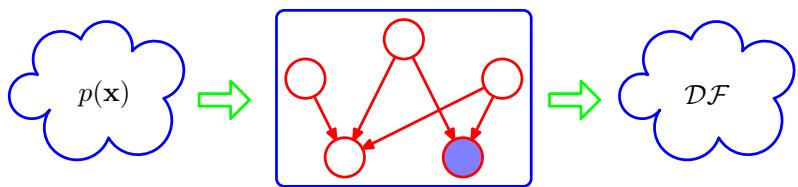
\includegraphics[keepaspectratio,alt={image}]{images/7b72877104f7a3ba02ac4808e1d547b6c91a30d5ea0996d244133843fe51e6f2.jpg}}

Figure 8.25 We can view a graphical model (in this case a directed
graph) as a filter in which a probability distribution
\(p ( \mathbf { x } )\) is allowed through the filter if, and only if,
it satisfies the directed factorization property (8.5). The set of all
possible probability distributions \(p ( \mathbf { x } )\) that pass
through the filter is denoted . We can alternatively use the graph to
filter distributions according to whether they respect all of the
conditional independencies implied by the d-separation properties of the
graph. The d-separation theorem says that it is the same set of
distributions \(\mathcal { D F }\) that will be allowed through this
second kind of filter.

Note that for any given graph, the set of distributions
\(\mathcal { D F }\) will include any distributions that have additional
independence properties beyond those described by the graph. For
instance, a fully factorized distribution will always be passed through
the filter implied by any graph over the corresponding set of variables.

We end our discussion of conditional independence properties by
exploring the concept of a Markov blanket or Markov boundary. Consider a
joint distribution
\(p ( \mathbf { x } _ { 1 } , \ldots , \mathbf { x } _ { D } )\)
represented by a directed graph having D nodes, and consider the
conditional distribution of a particular node with variables
\(\mathbf { x } _ { i }\) conditioned on all of the remaining variables
\(\mathbf { x } _ { j \neq i }\) . Using the factorization property
(8.5), we can express this conditional distribution in the form

\[
\begin{array}{r c l} p (\mathbf {x} _ {i} | \mathbf {x} _ {\{j \neq i \}}) & = & \frac {p (\mathbf {x} _ {1} , \ldots , \mathbf {x} _ {D})}{\int p (\mathbf {x} _ {1} , \ldots , \mathbf {x} _ {D})   \mathrm{d} \mathbf {x} _ {i}} \\ & = & \frac {\prod_ {k} p (\mathbf {x} _ {k} | \mathrm{pa} _ {k})}{\int \prod_ {k} p (\mathbf {x} _ {k} | \mathrm{pa} _ {k})   \mathrm{d} \mathbf {x} _ {i}} \end{array}
\]

in which the integral is replaced by a summation in the case of discrete
variables. We now observe that any factor
\(p ( \mathbf { x } _ { k } | \mathrm { p a } _ { k } )\) that does not
have any functional dependence on \(\mathbf { x } _ { i }\) can be taken
outside the integral over \(\mathbf { x } _ { i } .\) , and will
therefore cancel between numerator and denominator. The only factors
that remain will be the conditional distribution
\(p ( \mathbf { x } _ { i } | \mathrm { p a } _ { i } )\) for node
\(\mathbf { x } _ { i }\) itself, together with the conditional
distributions for any nodes \(\mathbf { x } _ { k }\) such that node
\(\mathbf { x } _ { i }\) is in the conditioning set of
\(p ( \mathbf { x } _ { k } | \mathrm { p a } _ { k } )\) , in other
words for which \(\mathbf { x } _ { i }\) is a parent of
\(\mathbf { x } _ { k }\) . The conditional
\(p ( \mathbf { x } _ { i } | \mathrm { p a } _ { i } )\) will depend on
the parents of node \(\mathbf { x } _ { i } .\) , whereas the
conditionals \(p ( \mathbf { x } _ { k } | \mathrm { p a } _ { k } )\)
will depend on the children

Figure 8.26

The Markov blanket of a node \(\mathbf { x } _ { i }\) comprises the set
of parents, children and co-parents of the node. It has the property
that the conditional distribution of \(\mathbf { x } _ { i } ,\) ,
conditioned on all the remaining variables in the graph, is dependent
only on the variables in the Markov blanket.

\pandocbounded{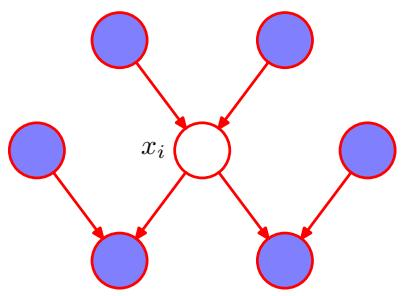
\includegraphics[keepaspectratio,alt={image}]{images/1278c7dba0a31f834f72e49d4e997dee2c9f0d8ae5554fe85e0fec702d084ea3.jpg}}

of \(\mathbf { x } _ { i }\) as well as on the co-parents, in other
words variables corresponding to parents of node
\(\mathbf { x } _ { k }\) other than node \(\mathbf { x } _ { i }\) .
The set of nodes comprising the parents, the children and the co-parents
is called the Markov blanket and is illustrated in Figure 8.26. We can
think of the Markov blanket of a node \(\mathbf { x } _ { i }\) as being
the minimal set of nodes that isolates \(\mathbf { x } _ { i }\) from
the rest of the graph. Note that it is not sufficient to include only
the parents and children of node \(\mathbf { x } _ { i }\) because the
phenomenon of explaining away means that observations of the child nodes
will not block paths to the co-parents. We must therefore observe the
co-parent nodes also.

\subsection{8.3. Markov Random Fields}\label{markov-random-fields}

We have seen that directed graphical models specify a factorization of
the joint distribution over a set of variables into a product of local
conditional distributions. They also define a set of conditional
independence properties that must be satisfied by any distribution that
factorizes according to the graph. We turn now to the second major class
of graphical models that are described by undirected graphs and that
again specify both a factorization and a set of conditional independence
relations.

A Markov random field, also known as a Markov network or an undirected
graphical model (Kindermann and Snell, 1980), has a set of nodes each of
which corresponds to a variable or group of variables, as well as a set
of links each of which connects a pair of nodes. The links are
undirected, that is they do not carry arrows. In the case of undirected
graphs, it is convenient to begin with a discussion of conditional
independence properties.

\subsection{8.3.1 Conditional independence
properties}\label{conditional-independence-properties}

In the case of directed graphs, we saw that it was possible to test
whether a particular conditional independence property holds by applying
a graphical test called d-separation. This involved testing whether or
not the paths connecting two sets of nodes were `blocked'. The
definition of blocked, however, was somewhat subtle due to the presence
of paths having head-to-head nodes. We might ask whether it is possible
to define an alternative graphical semantics for probability
distributions such that conditional independence is determined by simple
graph separation. This is indeed the case and corresponds to undirected
graphical models. By removing the

An example of an undirected graph in which every path from any node in
set A to any node in set B passes through at least one node in set C.
Consequently the conditional independence property A B C holds for any
probability distribution described by this graph.

\pandocbounded{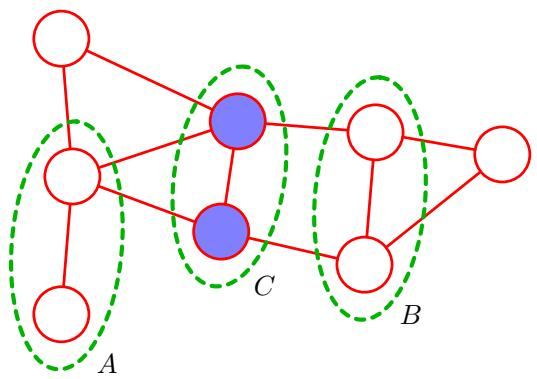
\includegraphics[keepaspectratio,alt={image}]{images/cbda658247a26ff9a9525e09d92dd46524d1193b4c09c2b3d3baafc119397389.jpg}}

directionality from the links of the graph, the asymmetry between parent
and child nodes is removed, and so the subtleties associated with
head-to-head nodes no longer arise.

Suppose that in an undirected graph we identify three sets of nodes,
denoted A, \(B ,\) and \(C ,\) , and that we consider the conditional
independence property

\[
A \perp \perp B \mid C.\tag{8.37}
\]

To test whether this property is satisfied by a probability distribution
defined by a graph we consider all possible paths that connect nodes in
set A to nodes in set B. If all such paths pass through one or more
nodes in set C, then all such paths are `blocked' and so the conditional
independence property holds. However, if there is at least one such path
that is not blocked, then the property does not necessarily hold, or
more precisely there will exist at least some distributions
corresponding to the graph that do not satisfy this conditional
independence relation. This is illustrated with an example in Figure
8.27. Note that this is exactly the same as the d-separation criterion
except that there is no `explaining away' phenomenon. Testing for
conditional independence in undirected graphs is therefore simpler than
in directed graphs.

An alternative way to view the conditional independence test is to
imagine removing all nodes in set C from the graph together with any
links that connect to those nodes. We then ask if there exists a path
that connects any node in A to any node in B. If there are no such
paths, then the conditional independence property must hold.

The Markov blanket for an undirected graph takes a particularly simple
form, because a node will be conditionally independent of all other
nodes conditioned only on the neighbouring nodes, as illustrated in
Figure 8.28.

\subsection{8.3.2 Factorization
properties}\label{factorization-properties}

We now seek a factorization rule for undirected graphs that will
correspond to the above conditional independence test. Again, this will
involve expressing the joint distribution \(p ( \mathbf { x } )\) as a
product of functions defined over sets of variables that are local to
the graph. We therefore need to decide what is the appropriate notion of
locality in this case.

Figure 8.28 For an undirected graph, the Markov blanket of a node
\(x _ { i }\) consists of the set of neighbouring nodes. It has the
property that the conditional distribution of \(x _ { i } ,\) ,
conditioned on all the remaining variables in the graph, is dependent
only on the variables in the Markov blanket.

\pandocbounded{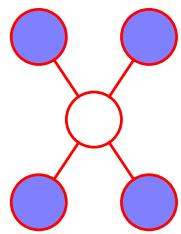
\includegraphics[keepaspectratio,alt={image}]{images/fae0de263b51fd7fd19a5c69b3b55ac8bce1dccd19174bdf03c6f115b70e74af.jpg}}

If we consider two nodes \(x _ { i }\) and \(x _ { j }\) that are not
connected by a link, then these variables must be conditionally
independent given all other nodes in the graph. This follows from the
fact that there is no direct path between the two nodes, and all other
paths pass through nodes that are observed, and hence those paths are
blocked. This conditional independence property can be expressed as

\[
p (x _ {i}, x _ {j} | \mathbf {x} _ {\backslash \{i, j \}}) = p (x _ {i} | \mathbf {x} _ {\backslash \{i, j \}}) p (x _ {j} | \mathbf {x} _ {\backslash \{i, j \}})\tag{8.38}
\]

where \$\mathbf { x } \_ \langle ~i , j \} \$ denotes the set x of all
variables with \(x _ { i }\) and \(x _ { j }\) removed. The
factorization of the joint distribution must therefore be such that
\(x _ { i }\) and \(x _ { j }\) do not appear in the same factor in
order for the conditional independence property to hold for all possible
distributions belonging to the graph.

This leads us to consider a graphical concept called a clique, which is
defined as a subset of the nodes in a graph such that there exists a
link between all pairs of nodes in the subset. In other words, the set
of nodes in a clique is fully connected. Furthermore, a maximal clique
is a clique such that it is not possible to include any other nodes from
the graph in the set without it ceasing to be a clique. These concepts
are illustrated by the undirected graph over four variables shown in
Figure 8.29. This graph has five cliques of two nodes given by
\(\{ x _ { 1 } , x _ { 2 } \} , \{ x _ { 2 } , x _ { 3 } \} , \{ x _ { 3 } , x _ { 4 } \} , \{ x _ { 4 } , x _ { 2 } \}\)
and \(\{ x _ { 1 } , x _ { 3 } \}\) , as well as two maximal cliques
given by \(\{ x _ { 1 } , x _ { 2 } , x _ { 3 } \}\) and
\(\{ x _ { 2 } , x _ { 3 } , x _ { 4 } \}\) The set
\(\{ x _ { 1 } , x _ { 2 } , x _ { 3 } , x _ { 4 } \}\) is not a clique
because of the missing link from
\(x _ { 1 } ~ \mathrm { t o } ~ x _ { 4 }\)

We can therefore define the factors in the decomposition of the joint
distribution to be functions of the variables in the cliques. In fact,
we can consider functions of the maximal cliques, without loss of
generality, because other cliques must be subsets of maximal cliques.
Thus, if \(\{ x _ { 1 } , x _ { 2 } , x _ { 3 } \}\) is a maximal clique
and we define an arbitrary function over this clique, then including
another factor defined over a subset of these variables would be
redundant.

Let us denote a clique by \(C\) and the set of variables in that clique
by \(\mathbf { x } _ { C }\) . Then

Figure 8.29

A four-node undirected graph showing a clique (outlined in green) and a
maximal clique (outlined in blue).

\pandocbounded{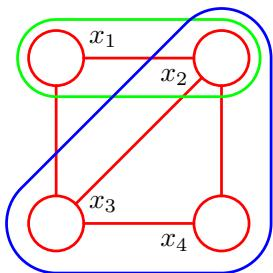
\includegraphics[keepaspectratio,alt={image}]{images/063699e13f1afab5018463eb1a81813f8e777f126872bd9cc89420bb6e032064.jpg}}

the joint distribution is written as a product of potential functions
\(\psi _ { C } ( \mathbf { x } _ { C } )\) over the maximal cliques of
the graph

\[
p (\mathbf {x}) = \frac {1}{Z} \prod_ {C} \psi_ {C} (\mathbf {x} _ {C}).\tag{8.39}
\]

Here the quantity \(Z ,\) sometimes called the partitionfunction, is a
normalization constant and is given by

\[
Z = \sum_ {\mathbf {x}} \prod_ {C} \psi_ {C} (\mathbf {x} _ {C})\tag{8.40}
\]

which ensures that the distribution \(p ( \mathbf { x } )\) given by
(8.39) is correctly normalized. By considering only potential functions
which satisfy \(\psi _ { C } ( \mathbf { x } _ { C } ) \geqslant 0\) we
ensure that \(p ( \mathbf { x } ) \geqslant 0\) . In (8.40) we have
assumed that x comprises discrete variables, but the framework is
equally applicable to continuous variables, or a combination of the two,
in which the summation is replaced by the appropriate combination of
summation and integration.

Note that we do not restrict the choice of potential functions to those
that have a specific probabilistic interpretation as marginal or
conditional distributions. This is in contrast to directed graphs in
which each factor represents the conditional distribution of the
corresponding variable, conditioned on the state of its parents.
However, in special cases, for instance where the undirected graph is
constructed by starting with a directed graph, the potential functions
may indeed have such an interpretation, as we shall see shortly.

One consequence of the generality of the potential functions
\(\psi _ { C } ( \mathbf { x } _ { C } )\) is that their product will in
general not be correctly normalized. We therefore have to introduce an
explicit normalization factor given by (8.40). Recall that for directed
graphs, the joint distribution was automatically normalized as a
consequence of the normalization of each of the conditional
distributions in the factorization.

The presence of this normalization constant is one of the major
limitations of undirected graphs. If we have a model with M discrete
nodes each having K states, then the evaluation of the normalization
term involves summing over \(K ^ { M }\) states and so (in the worst
case) is exponential in the size of the model. The partition function is
needed for parameter learning because it will be a function of any
parameters that govern the potential functions
\(\psi _ { C } ( \mathbf { x } _ { C } )\) . However, for evaluation of
local conditional distributions, the partition function is not needed
because a conditional is the ratio of two marginals, and the partition
function cancels between numerator and denominator when evaluating this
ratio. Similarly, for evaluating local marginal probabilities we can
work with the unnormalized joint distribution and then normalize the
marginals explicitly at the end. Provided the marginals only involves a
small number of variables, the evaluation of their normalization
coefficient will be feasible.

So far, we have discussed the notion of conditional independence based
on simple graph separation and we have proposed a factorization of the
joint distribution that is intended to correspond to this conditional
independence structure. However, we have not made any formal connection
between conditional independence and factorization for undirected
graphs. To do so we need to restrict attention to potential functions
\(\psi _ { C } ( \mathbf { x } _ { C } )\) that are strictly positive
(i.e., never zero or negative for any choice of
\(\mathbf { x } _ { C } )\) . Given this restriction, we can make a
precise relationship between factorization and conditional independence.

To do this we again return to the concept of a graphical model as a
filter, corresponding to Figure 8.25. Consider the set of all possible
distributions defined over a fixed set of variables corresponding to the
nodes of a particular undirected graph. We can define to be the set of
such distributions that are consistent with the set of conditional
independence statements that can be read from the graph using graph
separation. Similarly, we can define \(\mathcal { U F }\) to be the set
of such distributions that can be expressed as a factorization of the
form (8.39) with respect to the maximal cliques of the graph. The
Hammersley-Clifford theorem (Clifford, 1990) states that the sets and
\(\mathcal { U F }\) are identical.

Because we are restricted to potential functions which are strictly
positive it is convenient to express them as exponentials, so that

\[
\psi_ {C} (\mathbf {x} _ {C}) = \exp \left\{- E (\mathbf {x} _ {C}) \right\}\tag{8.41}
\]

where \(E ( \mathbf { x } _ { C } )\) is called an energy function, and
the exponential representation is called the Boltzmann distribution. The
joint distribution is defined as the product of potentials, and so the
total energy is obtained by adding the energies of each of the maximal
cliques.

In contrast to the factors in the joint distribution for a directed
graph, the potentials in an undirected graph do not have a specific
probabilistic interpretation. Although this gives greater flexibility in
choosing the potential functions, because there is no normalization
constraint, it does raise the question of how to motivate a choice of
potential function for a particular application. This can be done by
viewing the potential function as expressing which configurations of the
local variables are preferred to others. Global configurations that have
a relatively high probability are those that find a good balance in
satisfying the (possibly conflicting) influences of the clique
potentials. We turn now to a specific example to illustrate the use of
undirected graphs.

\subsection{8.3.3 Illustration: Image
de-noising}\label{illustration-image-de-noising}

We can illustrate the application of undirected graphs using an example
of noise removal from a binary image (Besag, 1974; Geman and Geman,
1984; Besag, 1986). Although a very simple example, this is typical of
more sophisticated applications. Let the observed noisy image be
described by an array of binary pixel values \(y _ { i } \in\)
\(\{ - 1 , + 1 \}\) , where the index \(i = 1 , \ldots , D\) runs over
all pixels. We shall suppose that the image is obtained by taking an
unknown noise-free image, described by binary pixel values
\(x _ { i } \in \{ - 1 , + 1 \}\) and randomly flipping the sign of
pixels with some small probability. An example binary image, together
with a noise corrupted image obtained by flipping the sign of the pixels
with probability 10\%, is shown in Figure 8.30. Given the noisy image,
our goal is to recover the original noise-free image.

Because the noise level is small, we know that there will be a strong
correlation between \(x _ { i }\) and \(y _ { i }\) . We also know that
neighbouring pixels \(x _ { i }\) and \(x _ { j }\) in an image are
strongly correlated. This prior knowledge can be captured using the
Markov random field model whose undirected graph is shown in Figure
8.31. This graph has two types of cliques, each of which contains two
variables. The cliques of the form \(\{ x _ { i } , y _ { i } \}\) have
an associated energy function that expresses the correlation between
these variables. We choose a very simple energy function for these
cliques of the form \(- \eta x _ { i } y _ { i }\) where \(\eta\) is a
positive constant. This has the desired effect of giving a lower energy
(thus encouraging a higher probability) when \(x _ { i }\) and
\(y _ { i }\) have the same sign and a higher energy when they have the
opposite sign.

\pandocbounded{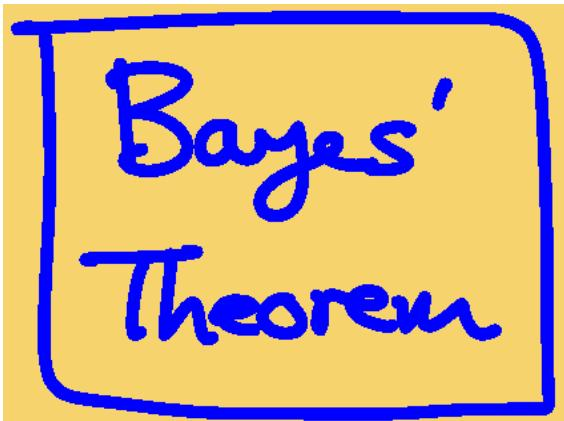
\includegraphics[keepaspectratio,alt={image}]{images/c87b905a56dfa4f35a30ec93a92d92b9fe2fefba729778de6f11f39368e4e2f1.jpg}}

\pandocbounded{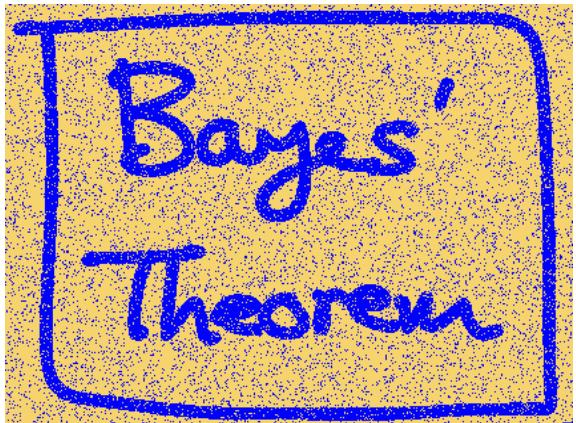
\includegraphics[keepaspectratio,alt={image}]{images/1aa1e04c033a20fe59a4c2e4b077f169de8be28cfbbe2628f860d13b4fd2e3cc.jpg}}

\pandocbounded{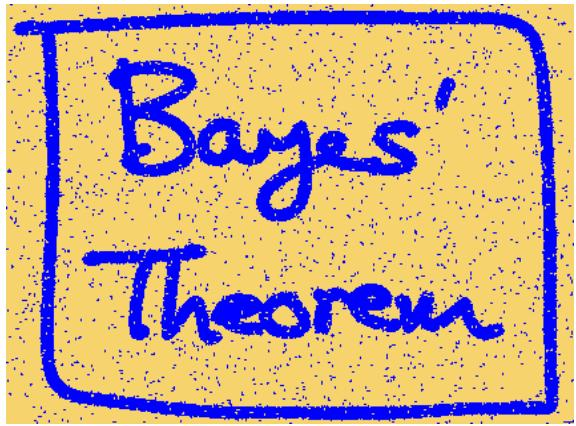
\includegraphics[keepaspectratio,alt={image}]{images/a207f2d30fa57249e95e22f3a440ad1603e928240e18348012f235986f3b0a0c.jpg}}

\pandocbounded{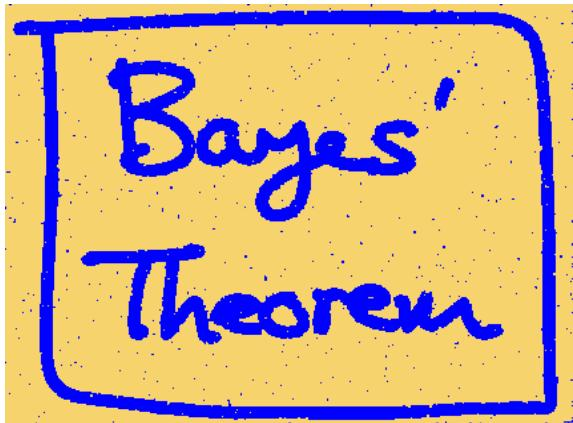
\includegraphics[keepaspectratio,alt={image}]{images/68ab7778d73161fc150ef01e017a6a37db97e149a8023f22b734cde251028ade.jpg}}

Figure 8.30 Illustration of image de-noising using a Markov random
field. The top row shows the original binary image on the left and the
corrupted image after randomly changing 10\% of the pixels on the right.
The bottom row shows the restored images obtained using iterated
conditional models (ICM) on the left and using the graph-cut algorithm
on the right. ICM produces an image where 96\% of the pixels agree with
the original image, whereas the corresponding number for graph-cut is
99\%.

The remaining cliques comprise pairs of variables
\(\{ x _ { i } , x _ { j } \}\) where \(i\) and \(j\) are indices of
neighbouring pixels. Again, we want the energy to be lower when the
pixels have the same sign than when they have the opposite sign, and so
we choose an energy given by \(\mathbf { - } \beta x _ { i } x _ { j }\)
where \(\beta\) is a positive constant.

Because a potential function is an arbitrary, nonnegative function over
a maximal clique, we can multiply it by any nonnegative functions of
subsets of the clique, or

An undirected graphical model representing a Markov random field for
image de-noising, in which \(x _ { i }\) is a binary variable denoting
the state of pixel i in the unknown noise-free image, and \(y _ { i }\)
denotes the corresponding value of pixel i in the observed noisy image.

\pandocbounded{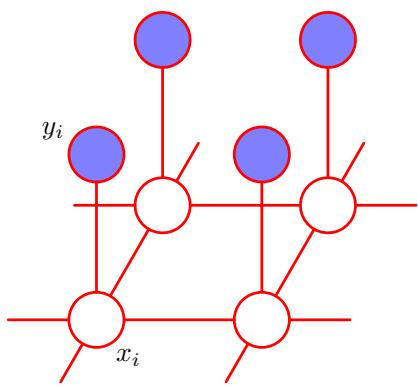
\includegraphics[keepaspectratio,alt={image}]{images/c3c088095d0c4dd3ef3b3c3014e33cb8bcc438c3d3333082a1a313b17fa5e1f2.jpg}}

equivalently we can add the corresponding energies. In this example,
this allows us to add an extra term \(h x _ { i }\) for each pixel i in
the noise-free image. Such a term has the effect of biasing the model
towards pixel values that have one particular sign in preference to the
other.

The complete energy function for the model then takes the form

\[
E (\mathbf {x}, \mathbf {y}) = h \sum_ {i} x _ {i} - \beta \sum_ {\{i, j \}} x _ {i} x _ {j} - \eta \sum_ {i} x _ {i} y _ {i}\tag{8.42}
\]

which defines a joint distribution over x and y given by

\[
p (\mathbf {x}, \mathbf {y}) = \frac {1}{Z} \exp \{- E (\mathbf {x}, \mathbf {y}) \}.\tag{8.43}
\]

We now fix the elements of \(\mathbf { y }\) to the observed values
given by the pixels of the noisy image, which implicitly defines a
conditional distribution \(p ( \mathbf { x } | \mathbf { y } )\) over
noisefree images. This is an example of the Ising model, which has been
widely studied in statistical physics. For the purposes of image
restoration, we wish to find an image x having a high probability
(ideally the maximum probability). To do this we shall use a simple
iterative technique called iterated conditional modes, or ICM (Kittler
and Foglein, 1984), which is simply an application of coordinate-wise
gradient ascent.¨ The idea is first to initialize the variables
\(\{ x _ { i } \}\) , which we do by simply setting \(x _ { i } =\)
\(y _ { i }\) for all i. Then we take one node \(x _ { j }\) at a time
and we evaluate the total energy for the two possible states
\(x _ { j } = + 1\) and \(x _ { j } = - 1\) , keeping all other node
variables fixed, and set \(x _ { j }\) to whichever state has the lower
energy. This will either leave the probability unchanged, if
\(x _ { j }\) is unchanged, or will increase it. Because only one
variable is changed, this is a simple local computation that can be
performed efficiently. We then repeat the update for another site, and
so on, until some suitable stopping criterion is satisfied. The nodes
may be updated in a systematic way, for instance by repeatedly raster
scanning through the image, or by choosing nodes at random.

If we have a sequence of updates in which every site is visited at least
once, and in which no changes to the variables are made, then by
definition the algorithm

Figure 8.32 graph. (b) graph.

\pandocbounded{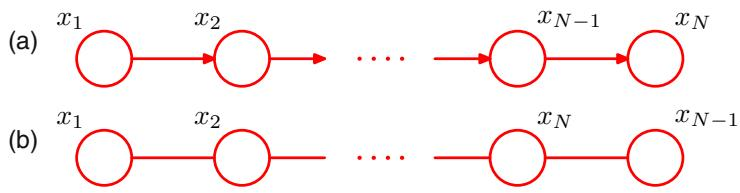
\includegraphics[keepaspectratio,alt={image}]{images/f4d6f5d5642c5089173544a2d9ed455787b17dde8ba5b71d344186db38d47833.jpg}}

will have converged to a local maximum of the probability. This need
not, however, correspond to the global maximum.

For the purposes of this simple illustration, we have fixed the
parameters to be \(\beta = 1 . 0 , \eta = 2 . 1\) and \(h = 0\) . Note
that leaving \(h = 0\) simply means that the prior probabilities of the
two states of \(x _ { i }\) are equal. Starting with the observed noisy
image as the initial configuration, we run ICM until convergence,
leading to the de-noised image shown in the lower left panel of Figure
8.30. Note that if we set \(\beta = 0\) which effectively removes the
links between neighbouring pixels, then the global most probable
solution is given by \(x _ { i } = y _ { i }\) for all i, corresponding
to the observed noisy image.

Later we shall discuss a more effective algorithm for finding high
probability solutions called the max-product algorithm, which typically
leads to better solutions, although this is still not guaranteed to find
the global maximum of the posterior distribution. However, for certain
classes of model, including the one given by (8.42), there exist
efficient algorithms based on graph cuts that are guaranteed to find the
global maximum (Greig et al., 1989; Boykov et al., 2001; Kolmogorov and
Zabih, 2004). The lower right panel of Figure 8.30 shows the result of
applying a graph-cut algorithm to the de-noising problem.

\subsection{8.3.4 Relation to directed
graphs}\label{relation-to-directed-graphs}

We have introduced two graphical frameworks for representing probability
distributions, corresponding to directed and undirected graphs, and it
is instructive to discuss the relation between these. Consider first the
problem of taking a model that is specified using a directed graph and
trying to convert it to an undirected graph. In some cases this is
straightforward, as in the simple example in Figure 8.32. Here the joint
distribution for the directed graph is given as a product of
conditionals in the form

\[
p (\mathbf {x}) = p (x _ {1}) p (x _ {2} | x _ {1}) p (x _ {3} | x _ {2}) \dots p (x _ {N} | x _ {N - 1}).\tag{8.44}
\]

Now let us convert this to an undirected graph representation, as shown
in Figure 8.32. In the undirected graph, the maximal cliques are simply
the pairs of neighbouring nodes, and so from (8.39) we wish to write the
joint distribution in the form

\[
p (\mathbf {x}) = \frac {1}{Z} \psi_ {1, 2} (x _ {1}, x _ {2}) \psi_ {2, 3} (x _ {2}, x _ {3}) \dots \psi_ {N - 1, N} (x _ {N - 1}, x _ {N}).\tag{8.45}
\]

Figure 8.33 Example of a simple directed graph (a) and the corresponding
moral graph (b).

\pandocbounded{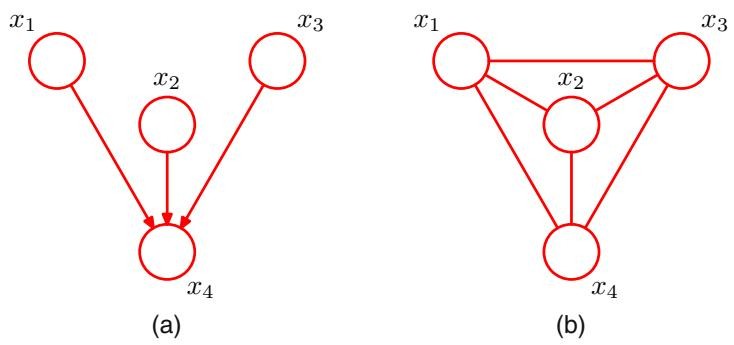
\includegraphics[keepaspectratio,alt={image}]{images/8f4b0f1a0906dd3e22a5e313a8b671f1c0ca0851db27be432146f7116f41eed5.jpg}}

This is easily done by identifying

\[
\begin{array}{r c l} \psi_ {1, 2} (x _ {1}, x _ {2}) & = & p (x _ {1}) p (x _ {2} | x _ {1}) \\ \psi_ {2, 3} (x _ {2}, x _ {3}) & = & p (x _ {3} | x _ {2}) \\ & \vdots \\ \psi_ {N - 1, N} (x _ {N - 1}, x _ {N}) & = & p (x _ {N} | x _ {N - 1}) \end{array}
\]

where we have absorbed the marginal \(p ( x _ { 1 } )\) for the first
node into the first potential function. Note that in this case, the
partition function \(Z = 1\)

Let us consider how to generalize this construction, so that we can
convert any distribution specified by a factorization over a directed
graph into one specified by a factorization over an undirected graph.
This can be achieved if the clique potentials of the undirected graph
are given by the conditional distributions of the directed graph. In
order for this to be valid, we must ensure that the set of variables
that appears in each of the conditional distributions is a member of at
least one clique of the undirected graph. For nodes on the directed
graph having just one parent, this is achieved simply by replacing the
directed link with an undirected link. However, for nodes in the
directed graph having more than one parent, this is not sufficient.
These are nodes that have `head-to-head' paths encountered in our
discussion of conditional independence. Consider a simple directed graph
over 4 nodes shown in Figure 8.33. The joint distribution for the
directed graph takes the form

\[
p (\mathbf {x}) = p (x _ {1}) p (x _ {2}) p (x _ {3}) p (x _ {4} | x _ {1}, x _ {2}, x _ {3}).\tag{8.46}
\]

We see that the factor
\(p ( x _ { 4 } | x _ { 1 } , x _ { 2 } , x _ { 3 } )\) involves the
four variables \(x _ { 1 } , x _ { 2 } , x _ { 3 }\) , and
\(x _ { 4 } .\) , and so these must all belong to a single clique if
this conditional distribution is to be absorbed into a clique potential.
To ensure this, we add extra links between all pairs of parents of the
node \(x _ { 4 }\) . Anachronistically, this process of `marrying the
parents' has become known as moralization, and the resulting undirected
graph, after dropping the arrows, is called the moral graph. It is
important to observe that the moral graph in this example is fully
connected and so exhibits no conditiona independence properties, in
contrast to the original directed graph.

Thus in general to convert a directed graph into an undirected graph, we
first add additional undirected links between all pairs of parents for
each node in the graph and then drop the arrows on the original links to
give the moral graph. Then we initialize all of the clique potentials of
the moral graph to 1. We then take each conditional distribution factor
in the original directed graph and multiply it into one of the clique
potentials. There will always exist at least one maximal clique that
contains all of the variables in the factor as a result of the
moralization step. Note that in all cases the partition function is
given by Z = 1.

The process of converting a directed graph into an undirected graph
plays an important role in exact inference techniques such as the
junction tree algorithm. Converting from an undirected to a directed
representation is much less common and in general presents problems due
to the normalization constraints.

We saw that in going from a directed to an undirected representation we
had to discard some conditional independence properties from the graph.
Of course, we could always trivially convert any distribution over a
directed graph into one over an undirected graph by simply using a fully
connected undirected graph. This would, however, discard all conditional
independence properties and so would be vacuous. The process of
moralization adds the fewest extra links and so retains the maximum
number of independence properties.

We have seen that the procedure for determining the conditional
independence properties is different between directed and undirected
graphs. It turns out that the two types of graph can express different
conditional independence properties, and it is worth exploring this
issue in more detail. To do so, we return to the view of a specific
(directed or undirected) graph as a filter, so that the set of all
possible distributions over the given variables could be reduced to a
subset that respects the conditional independencies implied by the
graph. A graph is said to be a D map (for `dependency map') of a
distribution if every conditional independence statement satisfied by
the distribution is reflected in the graph. Thus a completely
disconnected graph (no links) will be a trivial D map for any
distribution.

Alternatively, we can consider a specific distribution and ask which
graphs have the appropriate conditional independence properties. If
every conditional independence statement implied by a graph is satisfied
by a specific distribution, then the graph is said to be an I map (for
`independence map') of that distribution. Clearly a fully connected
graph will be a trivial I map for any distribution.

If it is the case that every conditional independence property of the
distribution is reflected in the graph, and vice versa, then the graph
is said to be a perfect map for

Venn diagram illustrating the set of all distributions P over a given
set of variables, together with the set of distributions D that can be
represented as a perfect map using a directed graph, and the set U that
can be represented as a perfect map using an undirected graph.

\pandocbounded{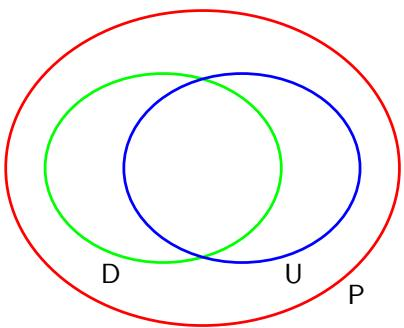
\includegraphics[keepaspectratio,alt={image}]{images/1a3fb693f2a3906f1eae46451bd2f27fd923aa356a13bf5f948ee29ea8187cc6.jpg}}

Figure 8.35 A directed graph whose conditional independence properties
cannot be expressed using an undirected graph over the same three
variables.

\pandocbounded{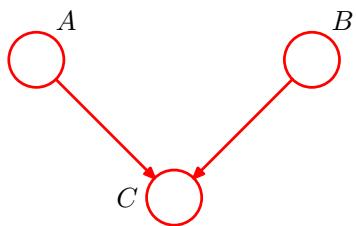
\includegraphics[keepaspectratio,alt={image}]{images/954ca23e019c9a1c714d6b0cb8ef6cabbb8334f73b3edc772d284714ddd59e1d.jpg}}

that distribution. A perfect map is therefore both an I map and a D map.

Consider the set of distributions such that for each distribution there
exists a directed graph that is a perfect map. This set is distinct from
the set of distributions such that for each distribution there exists an
undirected graph that is a perfect map. In addition there are
distributions for which neither directed nor undirected graphs offer a
perfect map. This is illustrated as a Venn diagram in Figure 8.34.

Figure 8.35 shows an example of a directed graph that is a perfect map
for a distribution satisfying the conditional independence properties
\({ \hat { A } } \perp \perp B \mid \emptyset\) and A B C. There is no
corresponding undirected graph over the same three variables that is a
perfect map.

Conversely, consider the undirected graph over four variables shown in
Figure 8.36. This graph exhibits the properties
\(A \mathbin { \downarrow } \chi \ B \ | \ \emptyset , C \mathbin { \downarrow } \bot \ D \ | \ A \cup B\)
and \(A \bot \bot B \mid C \cup D\) . There is no directed graph over
four variables that implies the same set of conditional independence
properties.

The graphical framework can be extended in a consistent way to graphs
that include both directed and undirected links. These are called chain
graphs (Lauritzen and Wermuth, 1989; Frydenberg, 1990), and contain the
directed and undirected graphs considered so far as special cases.
Although such graphs can represent a broader class of distributions than
either directed or undirected alone, there remain distributions for
which even a chain graph cannot provide a perfect map. Chain graphs are
not discussed further in this book.

An undirected graph whose conditional independence properties cannot be
expressed in terms of a directed graph over the same variables.

\pandocbounded{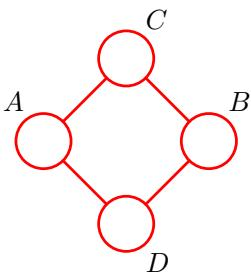
\includegraphics[keepaspectratio,alt={image}]{images/e9ecbcb3d8b9d0abd0ad31603a1ef58cd60aadf0f31cc9eee019573460e7632b.jpg}}

\subsection{8.4. Inference in Graphical
Models}\label{inference-in-graphical-models}

We turn now to the problem of inference in graphical models, in which
some of the nodes in a graph are clamped to observed values, and we wish
to compute the posterior distributions of one or more subsets of other
nodes. As we shall see, we can exploit the graphical structure both to
find efficient algorithms for inference, and

Figure 8.37 A graphical representation of Bayes' theorem. See the text
for details.

\pandocbounded{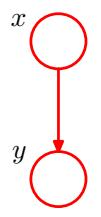
\includegraphics[keepaspectratio,alt={image}]{images/89abe895e22536c6c8d4eddd4e27d36e1d0a2ef11240381a4e7f9a402a04a8bd.jpg}}

\begin{enumerate}
\def\labelenumi{(\alph{enumi})}
\tightlist
\item
\end{enumerate}

\pandocbounded{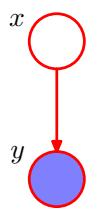
\includegraphics[keepaspectratio,alt={image}]{images/4a5044f9ab474a7b9056faafeaa11c2c4e6c32e981059e1723a43ed76418d1c4.jpg}}

\begin{enumerate}
\def\labelenumi{(\alph{enumi})}
\setcounter{enumi}{1}
\tightlist
\item
\end{enumerate}

\pandocbounded{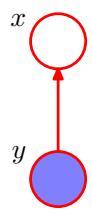
\includegraphics[keepaspectratio,alt={image}]{images/460a64192c9bd50deb60eb40dc864d6ebc7321627df3db2afcefe36eccf9702f.jpg}}

\begin{enumerate}
\def\labelenumi{(\alph{enumi})}
\setcounter{enumi}{2}
\tightlist
\item
\end{enumerate}

to make the structure of those algorithms transparent. Specifically, we
shall see that many algorithms can be expressed in terms of the
propagation of local messages around the graph. In this section, we
shall focus primarily on techniques for exact inference, and in Chapter
10 we shall consider a number of approximate inference algorithms.

To start with, let us consider the graphical interpretation of Bayes'
theorem. Suppose we decompose the joint distribution \(p ( x , y )\)
over two variables x and y into a product of factors in the form
\(p ( x , y ) = p ( x ) p ( y | x )\) . This can be represented by the
directed graph shown in Figure 8.37(a). Now suppose we observe the value
of \(y ,\) as indicated by the shaded node in Figure 8.37(b). We can
view the marginal distribution \(p ( x )\) as a prior over the latent
variable x, and our goal is to infer the corresponding posterior
distribution over x. Using the sum and product rules of probability we
can evaluate

\[
p (y) = \sum_ {x ^ {\prime}} p (y | x ^ {\prime}) p (x ^ {\prime})\tag{8.47}
\]

which can then be used in Bayes' theorem to calculate

\[
p (x | y) = \frac {p (y | x) p (x)}{p (y)}.\tag{8.48}
\]

Thus the joint distribution is now expressed in terms of \(p ( y )\) and
\(p ( x | y )\) . From a graphical perspective, the joint distribution
\(p ( x , y )\) is now represented by the graph shown in Figure 8.37(c),
in which the direction of the arrow is reversed. This is the simplest
example of an inference problem for a graphical model.

\subsection{8.4.1 Inference on a chain}\label{inference-on-a-chain}

Now consider a more complex problem involving the chain of nodes of the
form shown in Figure 8.32. This example will lay the foundation for a
discussion of exact inference in more general graphs later in this
section.

Specifically, we shall consider the undirected graph in Figure 8.32(b).
We have already seen that the directed chain can be transformed into an
equivalent undirected chain. Because the directed graph does not have
any nodes with more than one parent, this does not require the addition
of any extra links, and the directed and undirected versions of this
graph express exactly the same set of conditional independence
statements.

The joint distribution for this graph takes the form

\[
p (\mathbf {x}) = \frac {1}{Z} \psi_ {1, 2} (x _ {1}, x _ {2}) \psi_ {2, 3} (x _ {2}, x _ {3}) \dots \psi_ {N - 1, N} (x _ {N - 1}, x _ {N}).\tag{8.49}
\]

We shall consider the specific case in which the N nodes represent
discrete variables each having K states, in which case each potential
function \(\psi _ { n - 1 , n } ( x _ { n - 1 } , x _ { n } )\)
comprises an \(K \times K\) table, and so the joint distribution has
\(( N - 1 ) K ^ { 2 }\) parameters.

Let us consider the inference problem of finding the marginal
distribution \(p ( x _ { n } )\) for a specific node \(x _ { n }\) that
is part way along the chain. Note that, for the moment, there are no
observed nodes. By definition, the required marginal is obtained by
summing the joint distribution over all variables except \(x _ { n }\) ,
so that

\[
p (x _ {n}) = \sum_ {x _ {1}} \dots \sum_ {x _ {n - 1}} \sum_ {x _ {n + 1}} \dots \sum_ {x _ {N}} p (\mathbf {x}).\tag{8.50}
\]

In a naive implementation, we would first evaluate the joint
distribution and then perform the summations explicitly. The joint
distribution can be represented as a set of numbers, one for each
possible value for . Because there are N variables each with K states,
there are \(\dot { K ^ { N } }\) values for x and so evaluation and
storage of the joint distribution, as well as marginalization to obtain
\(p ( x _ { n } )\) , all involve storage and computation that scale
exponentially with the length N of the chain.

We can, however, obtain a much more efficient algorithm by exploiting
the conditional independence properties of the graphical model. If we
substitute the factorized expression (8.49) for the joint distribution
into (8.50), then we can rearrange the order of the summations and the
multiplications to allow the required marginal to be evaluated much more
efficiently. Consider for instance the summation over \(x _ { N }\) .
The potential \(\psi _ { N - 1 , N } ( x _ { N - 1 } , x _ { N } )\) is
the only one that depends on \(x _ { N }\) , and so we can perform the
summation

\[
\sum_ {x _ {N}} \psi_ {N - 1, N} (x _ {N - 1}, x _ {N})\tag{8.51}
\]

first to give a function of \(x _ { N - 1 }\) . We can then use this to
perform the summation over \(x _ { N - 1 }\) , which will involve only
this new function together with the potential
\(\psi _ { N - 2 , N - 1 } ( x _ { N - 2 } , x _ { N - 1 } )\) , because
this is the only other place that \(x _ { N - 1 }\) appears. Similarly,
the summation over \(x _ { 1 }\) involves only the potential
\(\psi _ { 1 , 2 } ( x _ { 1 } , x _ { 2 } )\) and so can be performed
separately to give a function of \(x _ { 2 }\) , and so on. Because each
summation effectively removes a variable from the distribution, this can
be viewed as the removal of a node from the graph.

If we group the potentials and summations together in this way, we can
express

the desired marginal in the form

\[
\begin{array}{l} p (x _ {n}) = \frac {1}{Z} \\ \underbrace {\left[ \sum_ {x _ {n - 1}} \psi_ {n - 1 , n} (x _ {n - 1} , x _ {n}) \cdots \left[ \sum_ {x _ {2}} \psi_ {2 , 3} (x _ {2} , x _ {3}) \left[ \sum_ {x _ {1}} \psi_ {1 , 2} (x _ {1} , x _ {2}) \right] \right] \cdots \right]} _ {\mu_ {\alpha} (x _ {n})} \\ \underbrace {\left[ \sum_ {x _ {n + 1}} \psi_ {n , n + 1} (x _ {n} , x _ {n + 1}) \cdots \left[ \sum_ {x _ {N}} \psi_ {N - 1 , N} (x _ {N - 1} , x _ {N}) \right] \cdots \right]} _ {\mu_ {\beta} (x _ {n})}. \end{array} \tag {8.5}\tag{8.52}
\]

The reader is encouraged to study this re-ordering carefully as the
underlying idea forms the basis for the later discussion of the general
sum-product algorithm. Here the key concept that we are exploiting is
that multiplication is distributive over addition, so that

\[
a b + a c = a (b + c)\tag{8.53}
\]

in which the left-hand side involves three arithmetic operations whereas
the righthand side reduces this to two operations.

Let us work out the computational cost of evaluating the required
marginal using this re-ordered expression. We have to perform \(N - 1\)
summations each of which is over \(K\) states and each of which involves
a function of two variables. For instance, the summation over
\(x _ { 1 }\) involves only the function
\(\psi _ { 1 , 2 } ( x _ { 1 } , x _ { 2 } )\) , which is a table of
\(K \times K\) numbers. We have to sum this table over \(x _ { 1 }\) for
each value of \(x _ { 2 }\) and so this has \(O ( K ^ { 2 } )\) cost.
The resulting vector of K numbers is multiplied by the matrix of numbers
\(\psi _ { 2 , 3 } ( x _ { 2 } , x _ { 3 } )\) and so is again
\(O ( K ^ { 2 } )\) ). Because there are \(N - 1\) summations and
multiplications of this kind, the total cost of evaluating the marginal
\(p ( x _ { n } )\) is \(O ( N K ^ { 2 } )\) . This is linear in the
length of the chain, in contrast to the exponential cost of a naive
approach. We have therefore been able to exploit the many conditional
independence properties of this simple graph in order to obtain an
efficient calculation. If the graph had been fully connected, there
would have been no conditional independence properties, and we would
have been forced to work directly with the full joint distribution.

We now give a powerful interpretation of this calculation in terms of
the passing of local messages around on the graph. From (8.52) we see
that the expression for the marginal \(p ( x _ { n } )\) decomposes into
the product of two factors times the normalization constant

\[
p (x _ {n}) = \frac {1}{Z} \mu_ {\alpha} (x _ {n}) \mu_ {\beta} (x _ {n}).\tag{8.54}
\]

We shall interpret \(\mu _ { \alpha } ( x _ { n } )\) as a message
passed forwards along the chain from node \(x _ { n - 1 }\) to node
\(x _ { n }\) . Similarly, \(\mu _ { \beta } ( x _ { n } )\) can be
viewed as a message passed backwards along the chain to node
\(x _ { n }\) from node \(x _ { n + 1 }\) . Note that each of the
messages comprises a set of K values, one for each choice of
\(x _ { n }\) , and so the product of two messages should be interpreted
as the point-wise multiplication of the elements of the two messages to
give another set of K values.

Figure 8.38 The marginal distribution \(p ( x _ { n } )\) for a node
\(x _ { n }\) along the chain is obtained by multiplying the two
messages \(\mu _ { \alpha } ( x _ { n } )\) and
\(\mu _ { \beta } ( x _ { n } )\) , and then normalizing. These messages
can themselves be evaluated recursively by passing messages from both
ends of the chain towards node \(x _ { n }\)

\pandocbounded{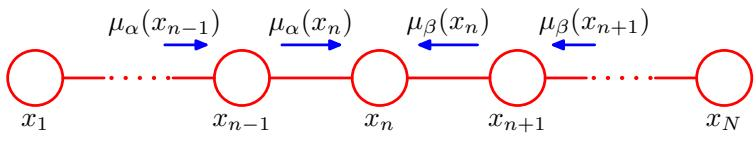
\includegraphics[keepaspectratio,alt={image}]{images/b51ebb20aaf16a8378a43bd1a9ac952ea9e7ba2235a78c83aa5b13a228e909bf.jpg}}

The message \(\mu _ { \alpha } ( x _ { n } )\) can be evaluated
recursively because

\[
\begin{array}{r c l} \mu_ {\alpha} (x _ {n}) & = & \sum_ {x _ {n - 1}} \psi_ {n - 1, n} (x _ {n - 1}, x _ {n}) \left[ \sum_ {x _ {n - 2}} \dots \right] \\ & = & \sum_ {x _ {n - 1}} \psi_ {n - 1, n} (x _ {n - 1}, x _ {n}) \mu_ {\alpha} (x _ {n - 1}). \end{array}\tag{8.55}
\]

We therefore first evaluate

\[
\mu_ {\alpha} (x _ {2}) = \sum_ {x _ {1}} \psi_ {1, 2} (x _ {1}, x _ {2})\tag{8.56}
\]

and then apply (8.55) repeatedly until we reach the desired node. Note
carefully the structure of the message passing equation. The outgoing
message \(\mu _ { \alpha } ( x _ { n } )\) in (8.55) is obtained by
multiplying the incoming message \(\mu _ { \alpha } ( x _ { n - 1 } )\)
by the local potential involving the node variable and the outgoing
variable and then summing over the node variable.

Similarly, the message \(\mu _ { \beta } ( x _ { n } )\) can be
evaluated recursively by starting with node \(x _ { N }\) and using

\[
\begin{array}{r c l} \mu_ {\beta} (x _ {n}) & = & \sum_ {x _ {n + 1}} \psi_ {n + 1, n} (x _ {n + 1}, x _ {n}) \left[ \sum_ {x _ {n + 2}} \dots \right] \\ & = & \sum_ {x _ {n + 1}} \psi_ {n + 1, n} (x _ {n + 1}, x _ {n}) \mu_ {\beta} (x _ {n + 1}). \end{array}\tag{8.57}
\]

This recursive message passing is illustrated in Figure 8.38. The
normalization constant \(Z\) is easily evaluated by summing the
right-hand side of (8.54) over all states of \(x _ { n }\) , an
operation that requires only \(O ( K )\) computation.

Graphs of the form shown in Figure 8.38 are called Markov chains, and
the corresponding message passing equations represent an example of the
Chapman-Kolmogorov equations for Markov processes (Papoulis, 1984).

Now suppose we wish to evaluate the marginals \(p ( x _ { n } )\) for
every node \(n \in\) \(\{ 1 , \ldots , N \}\) in the chain. Simply
applying the above procedure separately for each node will have
computational cost that is \(O ( N ^ { 2 } M ^ { 2 } )\) . However, such
an approach would be very wasteful of computation. For instance, to find
\(p ( x _ { 1 } )\) we need to propagate a message
\(\mu _ { \beta } ( \cdot )\) from node \(x _ { N }\) back to node
\(x _ { 2 }\) . Similarly, to evaluate \(p ( x _ { 2 } )\) we need to
propagate a messages \(\mu _ { \beta } ( \cdot )\) from node
\(x _ { N }\) back to node \(x _ { 3 }\) . This will involve much
duplicated computation because most of the messages will be identical in
the two cases.

Suppose instead we first launch a message
\(\mu _ { \beta } ( x _ { N - 1 } )\) starting from node \(x _ { N }\)
and propagate corresponding messages all the way back to node
\(x _ { 1 }\) , and suppose we similarly launch a message
\(\mu _ { \alpha } ( x _ { 2 } )\) starting from node \(x _ { 1 }\) and
propagate the corresponding messages all the way forward to node
\(x _ { N }\) . Provided we store all of the intermediate messages along
the way, then any node can evaluate its marginal simply by applying
(8.54). The computational cost is only twice that for finding the
marginal of a single node, rather than N times as much. Observe that a
message has passed once in each direction across each link in the graph.
Note also that the normalization constant \(Z\) need be evaluated only
once, using any convenient node.

If some of the nodes in the graph are observed, then the corresponding
variables are simply clamped to their observed values and there is no
summation. To see this, note that the effect of clamping a variable
\(x _ { n }\) to an observed value \({ \widehat { x } } _ { n }\) can be
expressed by multiplying the joint distribution by (one or more copies
of) an additional function \(I ( x _ { n } , { \widehat x } _ { n } )\)
, which takes the value 1 when
\(x _ { n } = { \widehat { x } } _ { n }\) and the value 0 otherwise.
One such function can then be absorbed into each of the potentials that
contain \(x _ { n }\) . Summations over \(x _ { n }\) then contain only
one term in which \(x _ { n } = { \widehat { x } } _ { n }\)

Now suppose we wish to calculate the joint distribution
\(p ( x _ { n - 1 } , x _ { n } )\) for two neighbouring nodes on the
chain. This is similar to the evaluation of the marginal for a single
node, except that there are now two variables that are not summed out. A
few moments thought will show that the required joint distribution can
be written in the form

\[
p (x _ {n - 1}, x _ {n}) = \frac {1}{Z} \mu_ {\alpha} (x _ {n - 1}) \psi_ {n - 1, n} (x _ {n - 1}, x _ {n}) \mu_ {\beta} (x _ {n}).\tag{8.58}
\]

Thus we can obtain the joint distributions over all of the sets of
variables in each of the potentials directly once we have completed the
message passing required to obtain the marginals.

This is a useful result because in practice we may wish to use
parametric forms for the clique potentials, or equivalently for the
conditional distributions if we started from a directed graph. In order
to learn the parameters of these potentials in situations where not all
of the variables are observed, we can employ the EM algorithm, and it
turns out that the local joint distributions of the cliques, conditioned
on any observed data, is precisely what is needed in the E step. We
shall consider some examples of this in detail in Chapter 13.

\subsection{8.4.2 Trees}\label{trees}

We have seen that exact inference on a graph comprising a chain of nodes
can be performed efficiently in time that is linear in the number of
nodes, using an algorithm that can be interpreted in terms of messages
passed along the chain. More generally, inference can be performed
efficiently using local message passing on a broader class of graphs
called trees. In particular, we shall shortly generalize the message
passing formalism derived above for chains to give the sum-product
algorithm, which provides an efficient framework for exact inference in
tree-structured graphs.

Figure 8.39 Examples of treestructured graphs, showing (a) an undirected
tree, (b) a directed tree, and (c) a directed polytree.

\pandocbounded{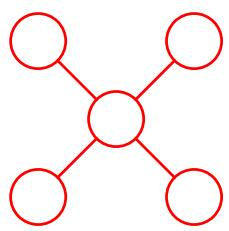
\includegraphics[keepaspectratio,alt={image}]{images/35b4c65676696b40cb36aa85a76eeb39a26ff73440c4664f7b3be096068865c7.jpg}}

\begin{enumerate}
\def\labelenumi{(\alph{enumi})}
\tightlist
\item
\end{enumerate}

\pandocbounded{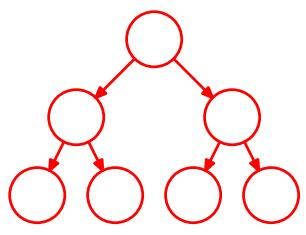
\includegraphics[keepaspectratio,alt={image}]{images/78767d695fadefe8fceb9cb9dfea1150e4e65d15592a51fcbef34e6ab893456b.jpg}}

\begin{enumerate}
\def\labelenumi{(\alph{enumi})}
\setcounter{enumi}{1}
\tightlist
\item
\end{enumerate}

\pandocbounded{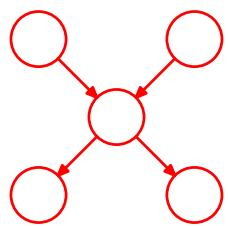
\includegraphics[keepaspectratio,alt={image}]{images/677d3d587e74c6c1d945b0b6e7418f007c91e7ca585b6e7a4fdaaed7369bdd1b.jpg}}

\begin{enumerate}
\def\labelenumi{(\alph{enumi})}
\setcounter{enumi}{2}
\tightlist
\item
\end{enumerate}

In the case of an undirected graph, a tree is defined as a graph in
which there is one, and only one, path between any pair of nodes. Such
graphs therefore do not have loops. In the case of directed graphs, a
tree is defined such that there is a single node, called the root, which
has no parents, and all other nodes have one parent. If we convert a
directed tree into an undirected graph, we see that the moralization
step will not add any links as all nodes have at most one parent, and as
a consequence the corresponding moralized graph will be an undirected
tree. Examples of undirected and directed trees are shown in Figure
8.39(a) and 8.39(b). Note that a distribution represented as a directed
tree can easily be converted into one represented by an undirected tree,
and vice versa.

If there are nodes in a directed graph that have more than one parent,
but there is still only one path (ignoring the direction of the arrows)
between any two nodes, then the graph is a called a polytree, as
illustrated in Figure 8.39(c). Such a graph will have more than one node
with the property of having no parents, and furthermore, the
corresponding moralized undirected graph will have loops.

\subsection{8.4.3 Factor graphs}\label{factor-graphs}

The sum-product algorithm that we derive in the next section is
applicable to undirected and directed trees and to polytrees. It can be
cast in a particularly simple and general form if we first introduce a
new graphical construction called a factor graph (Frey, 1998;
Kschischnang et al., 2001).

Both directed and undirected graphs allow a global function of several
variables to be expressed as a product of factors over subsets of those
variables. Factor graphs make this decomposition explicit by introducing
additional nodes for the factors themselves in addition to the nodes
representing the variables. They also allow us to be more explicit about
the details of the factorization, as we shall see.

Let us write the joint distribution over a set of variables in the form
of a product of factors

\[
p (\mathbf {x}) = \prod_ {s} f _ {s} (\mathbf {x} _ {s})\tag{8.59}
\]

where \(\mathbf { x } _ { s }\) denotes a subset of the variables. For
convenience, we shall denote the individual variables by \(x _ { i } ,\)
, however, as in earlier discussions, these can comprise groups of
variables (such as vectors or matrices). Each factor \(f _ { s }\) is a
function of a corresponding set of variables \(\mathbf { x } _ { s }\)

Figure 8.40 Example of a factor graph, which corresponds to the
factorization (8.60).

\pandocbounded{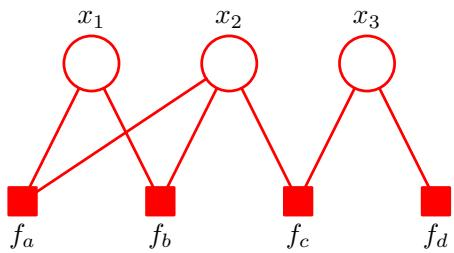
\includegraphics[keepaspectratio,alt={image}]{images/afada583cdf7afcb0180a33bdebaa1fc20845d12ed0e6eee5979c0aab443f1bf.jpg}}

Directed graphs, whose factorization is defined by (8.5), represent
special cases of (8.59) in which the factors
\(f _ { s } ( \mathbf { x } _ { s } )\) are local conditional
distributions. Similarly, undirected graphs, given by (8.39), are a
special case in which the factors are potential functions over the
maximal cliques (the normalizing coefficient \(1 / Z\) can be viewed as
a factor defined over the empty set of variables).

In a factor graph, there is a node (depicted as usual by a circle) for
every variable in the distribution, as was the case for directed and
undirected graphs. There are also additional nodes (depicted by small
squares) for each factor \(f _ { s } ( \mathbf { x } _ { s } )\) in the
joint distribution. Finally, there are undirected links connecting each
factor node to all of the variables nodes on which that factor depends.
Consider, for example, a distribution that is expressed in terms of the
factorization

\[
p (\mathbf {x}) = f _ {a} (x _ {1}, x _ {2}) f _ {b} (x _ {1}, x _ {2}) f _ {c} (x _ {2}, x _ {3}) f _ {d} (x _ {3}).\tag{8.60}
\]

This can be expressed by the factor graph shown in Figure 8.40. Note
that there are two factors \(f _ { a } ( x _ { 1 } , x _ { 2 } )\) and
\(f _ { b } ( x _ { 1 } , x _ { 2 } )\) that are defined over the same
set of variables. In an undirected graph, the product of two such
factors would simply be lumped together into the same clique potential.
Similarly, \(f _ { c } ( x _ { 2 } , x _ { 3 } )\) and
\(f _ { d } ( x _ { 3 } )\) could be combined into a single potential
over \(x _ { 2 }\) and \(x _ { 3 }\) . The factor graph, however, keeps
such factors explicit and so is able to convey more detailed information
about the underlying factorization.

\pandocbounded{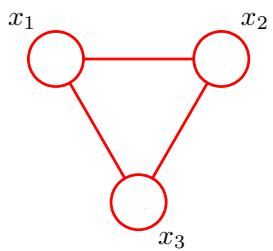
\includegraphics[keepaspectratio,alt={image}]{images/7664a07ee11313a2ac98e7d6cf8ea79e15719d3c360b1cd71ad6446908880b22.jpg}}

\begin{enumerate}
\def\labelenumi{(\alph{enumi})}
\tightlist
\item
\end{enumerate}

\pandocbounded{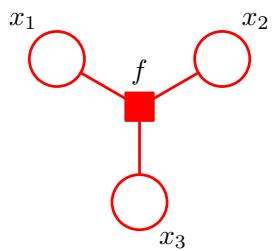
\includegraphics[keepaspectratio,alt={image}]{images/82fcd81b1275cdf3f8958a4966d8c73f854e6072620edec61a87106a12057d85.jpg}}

\begin{enumerate}
\def\labelenumi{(\alph{enumi})}
\setcounter{enumi}{1}
\tightlist
\item
\end{enumerate}

\pandocbounded{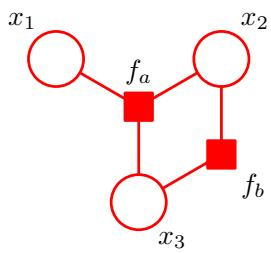
\includegraphics[keepaspectratio,alt={image}]{images/75d5c6447f5cc82e3f38608fd70fa0694bcd5f86b798e1e469d91162aa93a633.jpg}}

\begin{enumerate}
\def\labelenumi{(\alph{enumi})}
\setcounter{enumi}{2}
\tightlist
\item
\end{enumerate}

Figure 8.41 (a) An undirected graph with a single clique potential
\(\psi ( x _ { 1 } , x _ { 2 } , x _ { 3 } )\) . (b) A factor graph with
factor
\(f ( x _ { 1 } , x _ { 2 } , x _ { 3 } ) = \psi ( x _ { 1 } , x _ { 2 } , x _ { 3 } )\)
representing the same distribution as the undirected graph. (c) A
different factor graph representing the same distribution, whose factors
satisfy
\(f _ { a } ( x _ { 1 } , x _ { 2 } , x _ { 3 } ) f _ { b } ( x _ { 1 } , x _ { 2 } ) = \psi ( x _ { 1 } , x _ { 2 } , x _ { 3 } )\)

\pandocbounded{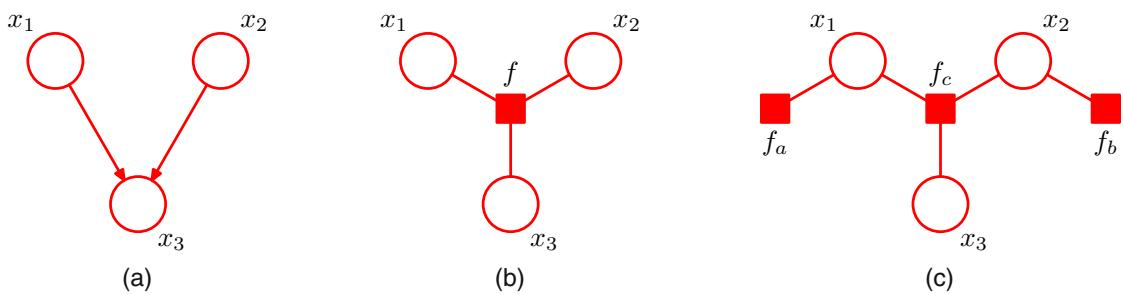
\includegraphics[keepaspectratio,alt={image}]{images/fde5e0c819a6ac51ad009064b1a99aabfe59b4300195f546e81ee5943a6a2a44.jpg}}

Figure 8.42 (a) A directed graph with the factorization
\(p ( x _ { 1 } ) p ( x _ { 2 } ) p ( x _ { 3 } | x _ { 1 } , x _ { 2 } )\)
. (b) A factor graph representing the same distribution as the directed
graph, whose factor satisfies
\(f ( x _ { 1 } , x _ { 2 } , x _ { 3 } ) = p ( x _ { 1 } ) p ( x _ { 2 } ) p ( x _ { 3 } | x _ { 1 } , x _ { 2 } )\)
. (c) A different factor graph representing the same distribution with
factors
\(f _ { a } ( x _ { 1 } ) \ : = \ : p ( x _ { 1 } ) , \ : f _ { b } ( x _ { 2 } ) \ : = \ : p ( x _ { 2 } )\)
and
\(f _ { c } ( x _ { 1 } , x _ { 2 } , x _ { 3 } ) = p ( x _ { 3 } | x _ { 1 } , x _ { 2 } )\)

Factor graphs are said to be bipartite because they consist of two
distinct kinds of nodes, and all links go between nodes of opposite
type. In general, factor graphs can therefore always be drawn as two
rows of nodes (variable nodes at the top and factor nodes at the bottom)
with links between the rows, as shown in the example in Figure 8.40. In
some situations, however, other ways of laying out the graph may be more
intuitive, for example when the factor graph is derived from a directed
or undirected graph, as we shall see.

If we are given a distribution that is expressed in terms of an
undirected graph, then we can readily convert it to a factor graph. To
do this, we create variable nodes corresponding to the nodes in the
original undirected graph, and then create additional factor nodes
corresponding to the maximal cliques \(\mathbf { x } _ { s }\) . The
factors \(f _ { s } ( \mathbf { x } _ { s } )\) are then set equal to
the clique potentials. Note that there may be several different factor
graphs that correspond to the same undirected graph. These concepts are
illustrated in Figure 8.41.

Similarly, to convert a directed graph to a factor graph, we simply
create variable nodes in the factor graph corresponding to the nodes of
the directed graph, and then create factor nodes corresponding to the
conditional distributions, and then finally add the appropriate links.
Again, there can be multiple factor graphs all of which correspond to
the same directed graph. The conversion of a directed graph to a factor
graph is illustrated in Figure 8.42.

We have already noted the importance of tree-structured graphs for
performing efficient inference. If we take a directed or undirected tree
and convert it into a factor graph, then the result will again be a tree
(in other words, the factor graph will have no loops, and there will be
one and only one path connecting any two nodes). In the case of a
directed polytree, conversion to an undirected graph results in loops
due to the moralization step, whereas conversion to a factor graph again
results in a tree, as illustrated in Figure 8.43. In fact, local cycles
in a directed graph due to links connecting parents of a node can be
removed on conversion to a factor graph by defining the appropriate
factor function, as shown in Figure 8.44.

We have seen that multiple different factor graphs can represent the
same directed or undirected graph. This allows factor graphs to be more
specific about the precise form of the factorization. Figure 8.45 shows
an example of a fully connected undirected graph along with two
different factor graphs. In (b), the joint distribution is given by a
general form
\(p ( \mathbf { x } ) = f ( x _ { 1 } , x _ { 2 } , x _ { 3 } )\) ,
whereas in (c), it is given by the more specific factorization
\(p ( { \bf x } ) = f _ { a } ( x _ { 1 } , x _ { 2 } ) f _ { b } ( x _ { 1 } , x _ { 3 } ) f _ { c } ( x _ { 2 } , x _ { 3 } )\)
. It should be emphasized that the factorization in (c) does not
correspond to any conditional independence properties.

\pandocbounded{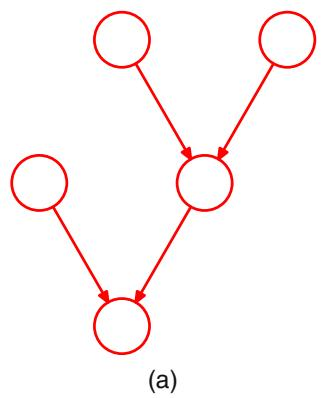
\includegraphics[keepaspectratio,alt={image}]{images/0c9db7073d1afa097ba73f33c1abda37fe65bcd6b1c56a809ccd081ac1667e46.jpg}}

\pandocbounded{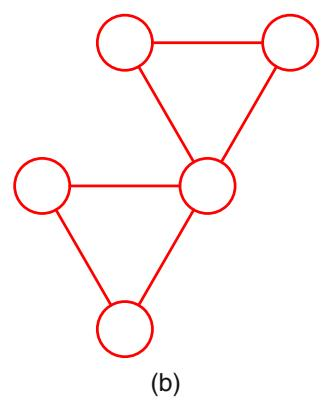
\includegraphics[keepaspectratio,alt={image}]{images/8dbbe2f69231f0114fd10566a38a15e7de97b0d94cc3107718d0299f6d71cb96.jpg}}

\pandocbounded{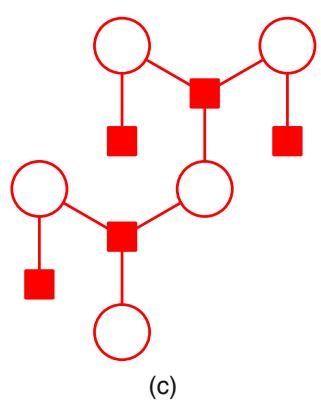
\includegraphics[keepaspectratio,alt={image}]{images/b08e4cbd2ee4d1d37ce86c69c5219e3c94df3267585662d030e985e92ca09687.jpg}}

Figure 8.43 (a) A directed polytree. (b) The result of converting the
polytree into an undirected graph showing the creation of loops. (c) The
result of converting the polytree into a factor graph, which retains the
tree structure.

\subsection{8.4.4 The sum-product
algorithm}\label{the-sum-product-algorithm}

We shall now make use of the factor graph framework to derive a powerful
class of efficient, exact inference algorithms that are applicable to
tree-structured graphs. Here we shall focus on the problem of evaluating
local marginals over nodes or subsets of nodes, which will lead us to
the sum-product algorithm. Later we shall modify the technique to allow
the most probable state to be found, giving rise to the max-sum
algorithm.

Also we shall suppose that all of the variables in the model are
discrete, and so marginalization corresponds to performing sums. The
framework, however, is equally applicable to linear-Gaussian models in
which case marginalization involves integration, and we shall consider
an example of this in detail when we discuss linear dynamical systems.

Figure 8.44

\begin{enumerate}
\def\labelenumi{(\alph{enumi})}
\tightlist
\item
  A fragment of a directed graph having a local cycle. (b) Conversion to
  a fragment of a factor graph having a tree structure, in which
  \(f ( x _ { 1 } , x _ { 2 } , x _ { 3 } ) =\)
  \(p ( x _ { 1 } ) p ( x _ { 2 } | x _ { 1 } ) p ( x _ { 3 } | x _ { 1 } , x _ { 2 } )\)
\end{enumerate}

\pandocbounded{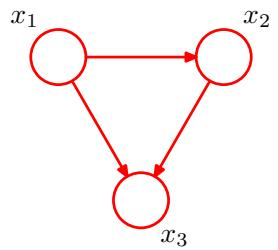
\includegraphics[keepaspectratio,alt={image}]{images/4b9f586a3c4d4087ee4ad929adc339b18c8fb9eecb8499c8a879e364ec114bde.jpg}}

\begin{enumerate}
\def\labelenumi{(\alph{enumi})}
\tightlist
\item
\end{enumerate}

\pandocbounded{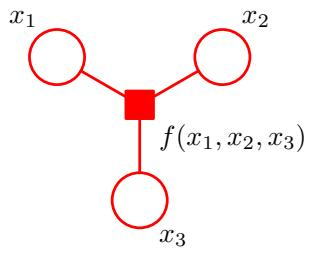
\includegraphics[keepaspectratio,alt={image}]{images/1f5f59fe368103648e7115a8dc9192b3b7528fb37fea33b198c74540a19e04a9.jpg}}

\begin{enumerate}
\def\labelenumi{(\alph{enumi})}
\setcounter{enumi}{1}
\tightlist
\item
\end{enumerate}

\pandocbounded{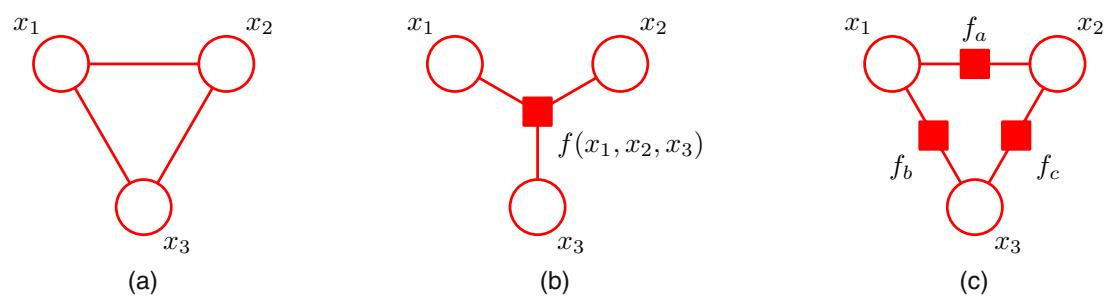
\includegraphics[keepaspectratio,alt={image}]{images/03273c091ead7e87a715665b9fc6bceec71c7b024c4a8fc15bf2734ae5ca2f49.jpg}}

Figure 8.45 (a) A fully connected undirected graph. (b) and (c) Two
factor graphs each of which corresponds to the undirected graph in (a).

There is an algorithm for exact inference on directed graphs without
loops known as belief propagation (Pearl, 1988; Lauritzen and
Spiegelhalter, 1988), and is equivalent to a special case of the
sum-product algorithm. Here we shall consider only the sum-product
algorithm because it is simpler to derive and to apply, as well as being
more general.

We shall assume that the original graph is an undirected tree or a
directed tree or polytree, so that the corresponding factor graph has a
tree structure. We first convert the original graph into a factor graph
so that we can deal with both directed and undirected models using the
same framework. Our goal is to exploit the structure of the graph to
achieve two things: (i) to obtain an efficient, exact inference
algorithm for finding marginals; (ii) in situations where several
marginals are required to allow computations to be shared efficiently.

We begin by considering the problem of finding the marginal \(p ( x )\)
for particular variable node x. For the moment, we shall suppose that
all of the variables are hidden. Later we shall see how to modify the
algorithm to incorporate evidence corresponding to observed variables.
By definition, the marginal is obtained by summing the joint
distribution over all variables except x so that

\[
p (x) = \sum_ {\mathbf {x} \backslash x} p (\mathbf {x})\tag{8.61}
\]

where \({ \textbf { x } } \backslash x\) denotes the set of variables in
x with variable x omitted. The idea is to substitute for
\(p ( \mathbf { x } )\) using the factor graph expression (8.59) and
then interchange summations and products in order to obtain an efficient
algorithm. Consider the fragment of graph shown in Figure 8.46 in which
we see that the tree structure of the graph allows us to partition the
factors in the joint distribution into groups, with one group associated
with each of the factor nodes that is a neighbour of the variable node
x. We see that the joint distribution can be written as a product of the
form

\[
p (\mathbf {x}) = \prod_ {s \in \mathrm{ne} (x)} F _ {s} (x, X _ {s})\tag{8.62}
\]

ne \(( x )\) denotes the set of factor nodes that are neighbours of
\(x ,\) and \(X _ { s }\) denotes the set of all variables in the
subtree connected to the variable node x via the factor node

Figure 8.46 A fragment of a factor graph illustrating the evaluation of
the marginal \(p ( x )\)

\pandocbounded{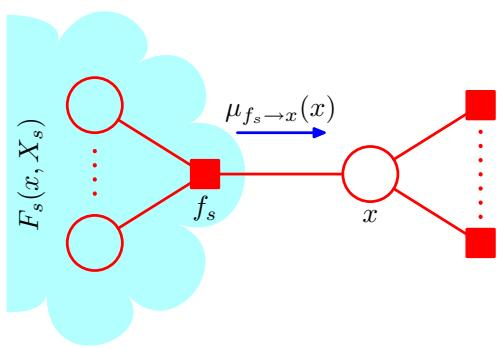
\includegraphics[keepaspectratio,alt={image}]{images/d8924513877f05d7b9b3f8476da10d339a57c0434ba6bef7bc50fe5f73f914ef.jpg}}

\(f _ { s } ,\) and \(F _ { s } ( x , X _ { s } )\) represents the
product of all the factors in the group associated with factor
\(f _ { s }\)

Substituting (8.62) into (8.61) and interchanging the sums and products,
we obtain

\[
\begin{array}{r c l} p (x) & = & \prod_ {s \in \mathrm{ne} (x)} \left[ \sum_ {X _ {s}} F _ {s} (x, X _ {s}) \right] \\ & = & \prod_ {s \in \mathrm{ne} (x)} \mu_ {f _ {s} \to x} (x). \end{array}\tag{8.63}
\]

Here we have introduced a set of functions
\(\mu _ { f _ { s } \to x } ( x )\) , defined by

\[
\mu_ {f _ {s} \rightarrow x} (x) \equiv \sum_ {X _ {s}} F _ {s} (x, X _ {s})\tag{8.64}
\]

which can be viewed as messages from the factor nodes \(f _ { s }\) to
the variable node x. We see that the required marginal \(p ( x )\) is
given by the product of all the incoming messages arriving at node x.

In order to evaluate these messages, we again turn to Figure 8.46 and
note that each factor \(F _ { s } ( x , X _ { s } )\) is described by a
factor (sub-)graph and so can itself be factorized. In particular, we
can write

\[
F _ {s} (x, X _ {s}) = f _ {s} (x, x _ {1}, \ldots , x _ {M}) G _ {1} \left(x _ {1}, X _ {s 1}\right) \ldots G _ {M} \left(x _ {M}, X _ {s M}\right)\tag{8.65}
\]

where, for convenience, we have denoted the variables associated with
factor \(f _ { x } ,\) , in addition to x, by
\(x _ { 1 } , \ldots , x _ { M }\) . This factorization is illustrated
in Figure 8.47. Note that the set of variables
\(\{ x , x _ { 1 } , \ldots , x _ { M } \}\) is the set of variables on
which the factor \(f _ { s }\) depends, and so it can also be denoted
\(\mathbf { x } _ { s }\) , using the notation of (8.59).

Substituting (8.65) into (8.64) we obtain

\[
\begin{array}{r c l}\mu_ {f _ {s} \rightarrow x} (x)&=&\sum_ {x _ {1}} \dots \sum_ {x _ {M}} f _ {s} (x, x _ {1}, \dots , x _ {M}) \prod_ {m \in \mathrm{ne} (f _ {s}) \backslash x} \left[ \sum_ {X _ {x m}} G _ {m} (x _ {m}, X _ {s m}) \right]\\&=&\sum_ {x _ {1}} \dots \sum_ {x _ {M}} f _ {s} (x, x _ {1}, \dots , x _ {M}) \prod_ {m \in \mathrm{ne} (f _ {s}) \backslash x} \mu_ {x _ {m} \rightarrow f _ {s}} (x _ {m})\end{array}\tag {8.6}
\]

Figure 8.47 Illustration of the factorization of the subgraph associated
with factor node \(f _ { s }\)

\pandocbounded{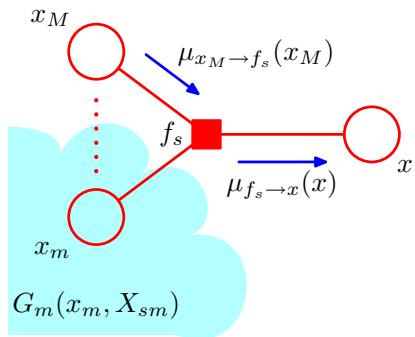
\includegraphics[keepaspectratio,alt={image}]{images/74e560390296edf2e7828b6a29fe6d0cc5fb558003752a477f433f83b7be975c.jpg}}

where \(\mathrm { n e } ( f _ { s } )\) denotes the set of variable
nodes that are neighbours of the factor node \(f _ { s } ,\) and ne
\(( f _ { s } ) \setminus x\) denotes the same set but with node x
removed. Here we have defined the following messages from variable nodes
to factor nodes

\[
\mu_ {x _ {m} \to f _ {s}} (x _ {m}) \equiv \sum_ {X _ {s m}} G _ {m} (x _ {m}, X _ {s m}).\tag{8.67}
\]

We have therefore introduced two distinct kinds of message, those that
go from factor nodes to variable nodes denoted \(\mu _ { f  x } ( x )\)
, and those that go from variable nodes to factor nodes denoted
\(\mu _ { x  f } ( x )\) . In each case, we see that messages passed
along a link are always a function of the variable associated with the
variable node that link connects to.

The result (8.66) says that to evaluate the message sent by a factor
node to a variable node along the link connecting them, take the product
of the incoming messages along all other links coming into the factor
node, multiply by the factor associated with that node, and then
marginalize over all of the variables associated with the incoming
messages. This is illustrated in Figure 8.47. It is important to note
that a factor node can send a message to a variable node once it has
received incoming messages from all other neighbouring variable nodes.

Finally, we derive an expression for evaluating the messages from
variable nodes to factor nodes, again by making use of the (sub-)graph
factorization. From Figure 8.48, we see that term
\(G _ { m } ( \bar { x } _ { m } , X _ { s m } )\) associated with node
\(x _ { m }\) is given by a product of terms
\(F _ { l } ( x _ { m } , X _ { m l } )\) each associated with one of
the factor nodes \(f _ { l }\) that is linked to node \(x _ { m }\)
(excluding node \(f _ { s } )\) , so that

\[
G _ {m} (x _ {m}, X _ {s m}) = \prod_ {l \in \mathrm{ne} (x _ {m}) \setminus f _ {s}} F _ {l} (x _ {m}, X _ {m l})\tag{8.68}
\]

where the product is taken over all neighbours of node \(x _ { m }\)
except for node \(f _ { s }\) . Note that each of the factors
\(F _ { l } ( x _ { m } , X _ { m l } )\) represents a subtree of the
original graph of precisely the same kind as introduced in (8.62).
Substituting (8.68) into (8.67), we

\begin{enumerate}
\def\labelenumi{(\alph{enumi})}
\tightlist
\item
\end{enumerate}

Figure 8.48 Illustration of the evaluation of the message sent by a
variable node to an adjacent factor node.

\pandocbounded{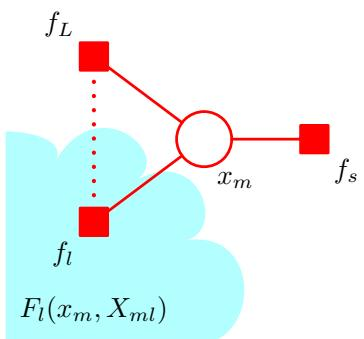
\includegraphics[keepaspectratio,alt={image}]{images/455c3f9f33dfc0c8a3b981d69e21328cc7426c7ddcd03bdf52d2f60d536e4db8.jpg}}

then obtain

\[
\begin{array}{r c l} \mu_ {x _ {m} \to f _ {s}} (x _ {m}) & = & \prod_ {l \in \mathrm{ne} (x _ {m}) \setminus f _ {s}} \left[ \sum_ {X _ {m l}} F _ {l} (x _ {m}, X _ {m l}) \right] \\ & = & \prod_ {l \in \mathrm{ne} (x _ {m}) \setminus f _ {s}} \mu_ {f _ {l} \to x _ {m}} (x _ {m}) \end{array}\tag{8.69}
\]

where we have used the definition (8.64) of the messages passed from
factor nodes to variable nodes. Thus to evaluate the message sent by a
variable node to an adjacent factor node along the connecting link, we
simply take the product of the incoming messages along all of the other
links. Note that any variable node that has only two neighbours performs
no computation but simply passes messages through unchanged. Also, we
note that a variable node can send a message to a factor node once it
has received incoming messages from all other neighbouring factor nodes.

Recall that our goal is to calculate the marginal for variable node x,
and that this marginal is given by the product of incoming messages
along all of the links arriving at that node. Each of these messages can
be computed recursively in terms of other messages. In order to start
this recursion, we can view the node x as the root of the tree and begin
at the leaf nodes. From the definition (8.69), we see that if a leaf
node is a variable node, then the message that it sends along its one
and only link is given by

\[
\mu_ {x \to f} (x) = 1\tag{8.70}
\]

as illustrated in Figure 8.49(a). Similarly, if the leaf node is a
factor node, we see from (8.66) that the message sent should take the
form

\[
\mu_ {f \to x} (x) = f (x)\tag{8.71}
\]

The sum-product algorithm begins with messages sent by the leaf nodes,
which depend on whether the leaf node is (a) a variable node, or (b) a
factor node.

\pandocbounded{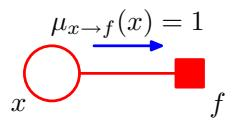
\includegraphics[keepaspectratio,alt={image}]{images/8767478bdd7694f7cdcf98be526eaae142ad16358c66a07ca5a1fce2ed57cdc7.jpg}}

\pandocbounded{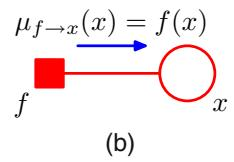
\includegraphics[keepaspectratio,alt={image}]{images/f3b846022bf952bf5bce0161cd1f9f5749e3c535098d0d6223f97275a782f87e.jpg}}

as illustrated in Figure 8.49(b).

At this point, it is worth pausing to summarize the particular version
of the sumproduct algorithm obtained so far for evaluating the marginal
\(p ( x )\) We start by viewing the variable node x as the root of the
factor graph and initiating messages at the leaves of the graph using
(8.70) and (8.71). The message passing steps (8.66) and (8.69) are then
applied recursively until messages have been propagated along every
link, and the root node has received messages from all of its
neighbours. Each node can send a message towards the root once it has
received messages from all of its other neighbours. Once the root node
has received messages from all of its neighbours, the required marginal
can be evaluated using (8.63). We shall illustrate this process shortly.

To see that each node will always receive enough messages to be able to
send out a message, we can use a simple inductive argument as follows.
Clearly, for a graph comprising a variable root node connected directly
to several factor leaf nodes, the algorithm trivially involves sending
messages of the form (8.71) directly from the leaves to the root. Now
imagine building up a general graph by adding nodes one at a time, and
suppose that for some particular graph we have a valid algorithm. When
one more (variable or factor) node is added, it can be connected only by
a single link because the overall graph must remain a tree, and so the
new node will be a leaf node. It therefore sends a message to the node
to which it is linked, which in turn will therefore receive all the
messages it requires in order to send its own message towards the root,
and so again we have a valid algorithm, thereby completing the proof.

Now suppose we wish to find the marginals for every variable node in the
graph. This could be done by simply running the above algorithm afresh
for each such node. However, this would be very wasteful as many of the
required computations would be repeated. We can obtain a much more
efficient procedure by `overlaying' these multiple message passing
algorithms to obtain the general sum-product algorithm as follows.
Arbitrarily pick any (variable or factor) node and designate it as the
root. Propagate messages from the leaves to the root as before. At this
point, the root node will have received messages from all of its
neighbours. It can therefore send out messages to all of its neighbours.
These in turn will then have received messages from all of their
neighbours and so can send out messages along the links going away from
the root, and so on. In this way, messages are passed outwards from the
root all the way to the leaves. By now, a message will have passed in
both directions across every link in the graph, and every node will have
received a message from all of its neighbours. Again a simple inductive
argument can be used to verify the validity of this message passing
protocol. Because every variable node will have received messages from
all of its neighbours, we can readily calculate the marginal
distribution for every variable in the graph. The number of messages
that have to be computed is given by twice the number of links in the
graph and so involves only twice the computation involved in finding a
single marginal. By comparison, if we had run the sum-product algorithm
separately for each node, the amount of computation would grow
quadratically with the size of the graph. Note that this algorithm is in
fact independent of which node was designated as the root,

The sum-product algorithm can be viewed purely in terms of messages sent
out by factor nodes to other factor nodes. In this example, the outgoing
message shown by the blue arrow is obtained by taking the product of all
the incoming messages shown by green arrows, multiplying by the factor
\(f _ { s }\) , and marginalizing over the variables \(x _ { 1 }\) and
\(x _ { 2 }\)

\pandocbounded{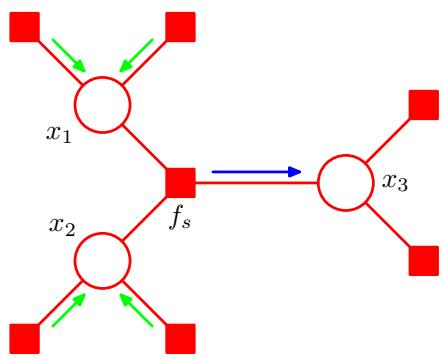
\includegraphics[keepaspectratio,alt={image}]{images/4c086c185deb3097dff23b11a6549c33496dac67d72588019a4bf778e1b88f81.jpg}}

and indeed the notion of one node having a special status was introduced
only as a convenient way to explain the message passing protocol.

Next suppose we wish to find the marginal distributions
\(p ( \mathbf { x } _ { s } )\) associated with the sets of variables
belonging to each of the factors. By a similar argument to that used
above, it is easy to see that the marginal associated with a factor is
given by the product of messages arriving at the factor node and the
local factor at that node

\[
p (\mathbf {x} _ {s}) = f _ {s} (\mathbf {x} _ {s}) \prod_ {i \in \mathrm{ne} (f _ {s})} \mu_ {x _ {i} \to f _ {s}} (x _ {i})\tag{8.72}
\]

in complete analogy with the marginals at the variable nodes. If the
factors are parameterized functions and we wish to learn the values of
the parameters using the EM algorithm, then these marginals are
precisely the quantities we will need to calculate in the E step, as we
shall see in detail when we discuss the hidden Markov model in Chapter
13.

The message sent by a variable node to a factor node, as we have seen,
is simply the product of the incoming messages on other links. We can if
we wish view the sum-product algorithm in a slightly different form by
eliminating messages from variable nodes to factor nodes and simply
considering messages that are sent out by factor nodes. This is most
easily seen by considering the example in Figure 8.50.

So far, we have rather neglected the issue of normalization. If the
factor graph was derived from a directed graph, then the joint
distribution is already correctly normalized, and so the marginals
obtained by the sum-product algorithm will similarly be normalized
correctly. However, if we started from an undirected graph, then in
general there will be an unknown normalization coefficient \(1 / Z\) .
As with the simple chain example of Figure 8.38, this is easily handled
by working with an unnormalized version
\(\widetilde { p } ( \mathbf { x } )\) of the joint distribution, where
\(p ( \mathbf { x } ) = \widetilde { p } ( \mathbf { x } ) / Z\) . We
first run the  sum-product algorithm to find the corresponding
unnormalized marginals
\(\widetilde { p } ( \boldsymbol { x } _ { i } )\) . The coefficient
\(1 / Z\) is then easily obtained by normalizing any one of these
marginals, and this is computationally efficient because the
normalization is done over a single variable rather than over the entire
set of variables as would be required to normalize
\(\widetilde { p } ( \mathbf { x } )\) directly.

At this point, it may be helpful to consider a simple example to
illustrate the operation of the sum-product algorithm. Figure 8.51 shows
a simple 4-node factor

Figure 8.51 A simple factor graph used to illustrate the sum-product
algorithm.

\pandocbounded{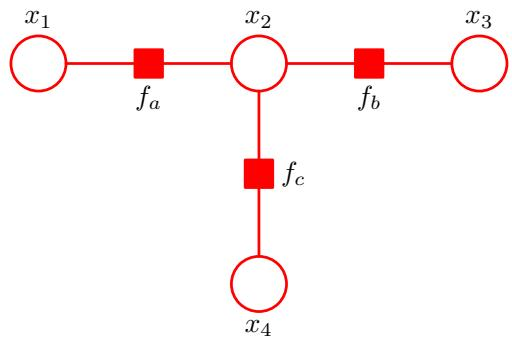
\includegraphics[keepaspectratio,alt={image}]{images/f61bc054fbfdd77d4eafcf8a12d5835a0cd4bfc11e3f4e3ba3260f793ab17e34.jpg}}

graph whose unnormalized joint distribution is given by

\[
\widetilde {p} (\mathbf {x}) = f _ {a} (x _ {1}, x _ {2}) f _ {b} (x _ {2}, x _ {3}) f _ {c} (x _ {2}, x _ {4}).\tag{8.73}
\]

In order to apply the sum-product algorithm to this graph, let us
designate node \(x _ { 3 }\) as the root, in which case there are two
leaf nodes \(x _ { 1 }\) and \(x _ { 4 }\) . Starting with the leaf
nodes, we then have the following sequence of six messages

\[
\mu_ {x _ {1} \to f _ {a}} (x _ {1}) = 1\tag{8.74}
\]

\[
\mu_ {f _ {a} \rightarrow x _ {2}} (x _ {2}) = \sum_ {x _ {1}} f _ {a} (x _ {1}, x _ {2})\tag{8.75}
\]

\[
\mu_ {x _ {4} \to f _ {c}} (x _ {4}) = 1\tag{8.76}
\]

\[
\mu_ {f _ {c} \to x _ {2}} (x _ {2}) = \sum_ {x _ {4}} f _ {c} (x _ {2}, x _ {4})\tag{8.77}
\]

\[
\mu_ {x _ {2} \to f _ {b}} (x _ {2}) = \mu_ {f _ {a} \to x _ {2}} (x _ {2}) \mu_ {f _ {c} \to x _ {2}} (x _ {2})\tag{8.78}
\]

\[
\mu_ {f _ {b} \to x _ {3}} (x _ {3}) = \sum_ {x _ {2}} f _ {b} (x _ {2}, x _ {3}) \mu_ {x _ {2} \to f _ {b}}.\tag{8.79}
\]

The direction of flow of these messages is illustrated in Figure 8.52.
Once this message propagation is complete, we can then propagate
messages from the root node out to the leaf nodes, and these are given
by

\[
\mu_ {x _ {3} \to f _ {b}} (x _ {3}) = 1\tag{8.80}
\]

\[
\mu_ {f _ {b} \rightarrow x _ {2}} (x _ {2}) = \sum_ {x _ {3}} f _ {b} (x _ {2}, x _ {3})\tag{8.81}
\]

\[
\mu_ {x _ {2} \to f _ {a}} (x _ {2}) = \mu_ {f _ {b} \to x _ {2}} (x _ {2}) \mu_ {f _ {c} \to x _ {2}} (x _ {2})\tag{8.82}
\]

\[
\mu_ {f _ {a} \to x _ {1}} (x _ {1}) = \sum_ {x _ {2}} f _ {a} (x _ {1}, x _ {2}) \mu_ {x _ {2} \to f _ {a}} (x _ {2})\tag{8.83}
\]

\[
\mu_ {x _ {2} \to f _ {c}} (x _ {2}) = \mu_ {f _ {a} \to x _ {2}} (x _ {2}) \mu_ {f _ {b} \to x _ {2}} (x _ {2})\tag{8.84}
\]

\[
\mu_ {f _ {c} \to x _ {4}} (x _ {4}) = \sum f _ {c} (x _ {2}, x _ {4}) \mu_ {x _ {2} \to f _ {c}} (x _ {2}).\tag{8.85}
\]

\pandocbounded{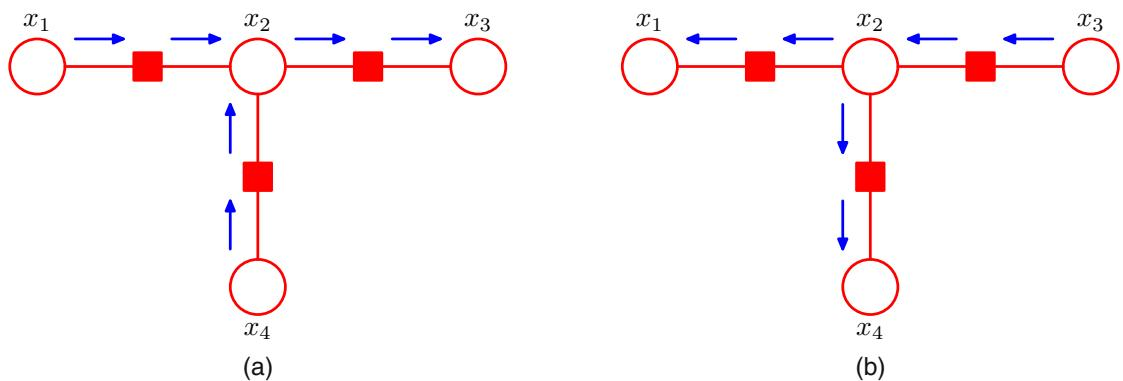
\includegraphics[keepaspectratio,alt={image}]{images/b2e367c00e007bfce3006a38f1fdce44f797669343780ea78f123a7e84f84dbd.jpg}}

Figure 8.52 Flow of messages for the sum-product algorithm applied to
the example graph in Figure 8.51. (a) From the leaf nodes \(x _ { 1 }\)
and \(x _ { 4 }\) towards the root node \(x _ { 3 }\) . (b) From the
root node towards the leaf nodes.

One message has now passed in each direction across each link, and we
can now evaluate the marginals. As a simple check, let us verify that
the marginal \(p ( x _ { 2 } )\) is given by the correct expression.
Using (8.63) and substituting for the messages using the above results,
we have

\[
\begin{array}{r c l} \widetilde {p} (x _ {2}) & = & \mu_ {f _ {a} \to x _ {2}} (x _ {2}) \mu_ {f _ {b} \to x _ {2}} (x _ {2}) \mu_ {f _ {c} \to x _ {2}} (x _ {2}) \\ & = & \left[ \sum_ {x _ {1}} f _ {a} (x _ {1}, x _ {2}) \right] \left[ \sum_ {x _ {3}} f _ {b} (x _ {2}, x _ {3}) \right] \left[ \sum_ {x _ {4}} f _ {c} (x _ {2}, x _ {4}) \right] \\ & = & \sum_ {x _ {1}} \sum_ {x _ {2}} \sum_ {x _ {4}} f _ {a} (x _ {1}, x _ {2}) f _ {b} (x _ {2}, x _ {3}) f _ {c} (x _ {2}, x _ {4}) \\ & = & \sum_ {x _ {1}} \sum_ {x _ {3}} \sum_ {x _ {4}} \widetilde {p} (\mathbf {x}) \end{array}\tag{8.86}
\]

as required.

So far, we have assumed that all of the variables in the graph are
hidden. In most practical applications, a subset of the variables will
be observed, and we wish to calculate posterior distributions
conditioned on these observations. Observed nodes are easily handled
within the sum-product algorithm as follows. Suppose we partition x into
hidden variables h and observed variables v, and that the observed value
of v is denoted \({ \widehat { \mathbf { v } } } .\) . Then we simply
multiply the joint distribution \(p ( \mathbf { x } )\) by
\(\textstyle \prod _ { i } I ( v _ { i } , { \widehat { v } } _ { i } )\)
where \(I ( v , \widehat { v } ) = 1\) if
\(\boldsymbol { v } = \boldsymbol { \hat { \hat { v } } }\) and
\(I ( v , \widehat { v } ) = \mathrm { 0 }\) otherwise. This product
corresponds to
\(p ( \mathbf { h } , \mathbf { v } = { \widehat { \mathbf { v } } } )\)
and hence is an unnormalized version of
\(p ( \mathbf { h } | \mathbf { v } = { \widehat { \mathbf { v } } } )\)
. By run- ning the sum-product algorithm, we can efficiently calculate
the posterior marginals
\(p ( h _ { i } | \mathbf { v } = { \widehat { \mathbf { v } } } )\) up
to a normalization coefficient whose value can be found efficiently
using a local computation. Any summations over variables in v then
collapse into a single term.

We have assumed throughout this section that we are dealing with
discrete variables. However, there is nothing specific to discrete
variables either in the graphical framework or in the probabilistic
construction of the sum-product algorithm. For

Table 8.1 Example of a joint distribution over two binary variables for
which the maximum of the joint distribution occurs for different
variable values compared to the maxima of the two marginals.

{\def\LTcaptype{none} % do not increment counter
\begin{longtable}[]{@{}|l|l|l|@{}}
\toprule\noalign{}
\endhead
\bottomrule\noalign{}
\endlastfoot
\hline
& x=0 & x=1 \\
\hline
y=0 & 0.3 & 0.4 \\
\hline
y=1 & 0.3 & 0.0 \\
\hline
\end{longtable}
}

continuous variables the summations are simply replaced by integrations.
We shall give an example of the sum-product algorithm applied to a graph
of linear-Gaussian variables when we consider linear dynamical systems.

\subsection{8.4.5 The max-sum algorithm}\label{the-max-sum-algorithm}

The sum-product algorithm allows us to take a joint distribution
\(p ( \mathbf { x } )\) expressed as a factor graph and efficiently find
marginals over the component variables. Two other common tasks are to
find a setting of the variables that has the largest probability and to
find the value of that probability. These can be addressed through a
closely related algorithm called max-sum, which can be viewed as an
application of dynamic programming in the context of graphical models
(Cormen et al., 2001).

A simple approach to finding latent variable values having high
probability would be to run the sum-product algorithm to obtain the
marginals \(p ( x _ { i } )\) for every variable, and then, for each
marginal in turn, to find the value \(x _ { i } ^ { \star }\) that
maximizes that marginal. However, this would give the set of values that
are individually the most probable. In practice, we typically wish to
find the set of values that jointly have the largest probability, in
other words the vector \(\mathbf { x } ^ { \mathrm { { m a x } } }\)
that maximizes the joint distribution, so that

\[
\mathbf {x} ^ {\max} = \underset {\mathbf {x}} {\arg \max} p (\mathbf {x})\tag{8.87}
\]

for which the corresponding value of the joint probability will be given
by

\[
p (\mathbf {x} ^ {\max}) = \max _ {\mathbf {x}} p (\mathbf {x}).\tag{8.88}
\]

In general, \(\mathbf { x } ^ { \mathrm { { m a x } } }\) is not the
same as the set of \(x _ { i } ^ { \star }\) values, as we can easily
show using a simple example. Consider the joint distribution
\(p ( x , y )\) over two binary variables \(x , y \in \{ 0 , 1 \}\)
given in Table 8.1. The joint distribution is maximized by setting
\(x =\) 1 and \(y = 0\) , corresponding the value 0.4. However, the
marginal for \(p ( x )\) , obtained by summing over both values of
\(y ,\) is given by \(p ( x = 0 ) = 0 . 6\) and \(p ( x = 1 ) = 0 . 4\)
and similarly the marginal for \(y\) is given by \(p ( y = 0 ) = 0 . 7\)
and \(p ( y = 1 ) = 0 . 3\) and so the marginals are maximized by
\(x = 0\) and \(y = 0\) , which corresponds to a value of 0.3 for the
joint distribution. In fact, it is not difficult to construct examples
for which the set of individually most probable values has probability
zero under the joint distribution.

We therefore seek an efficient algorithm for finding the value of x that
maximizes the joint distribution \(p ( \mathbf { x } )\) and that will
allow us to obtain the value of the joint distribution at its maximum.
To address the second of these problems, we shall simply write out the
max operator in terms of its components

\[
\max _ {\mathbf {x}} p (\mathbf {x}) = \max _ {x _ {1}} \ldots \max _ {x _ {M}} p (\mathbf {x})\tag{8.89}
\]

where M is the total number of variables, and then substitute for
\(p ( \mathbf { x } )\) using its expansion in terms of a product of
factors. In deriving the sum-product algorithm, we made use of the
distributive law (8.53) for multiplication. Here we make use of the
analogous law for the max operator

\[
\max (a b, a c) = a \max (b, c)\tag{8.90}
\]

which holds if \(a \geqslant 0\) (as will always be the case for the
factors in a graphical model). This allows us to exchange products with
maximizations.

Consider first the simple example of a chain of nodes described by
(8.49). The evaluation of the probability maximum can be written as

\[
\begin{array}{l} \underset {\mathbf {x}} {\max} p (\mathbf {x}) = \frac {1}{Z} \underset {x _ {1}} {\max} \dots \underset {x _ {N}} {\max} \left[ \psi_ {1, 2} (x _ {1}, x _ {2}) \dots \psi_ {N - 1, N} (x _ {N - 1}, x _ {N}) \right] \\ = \frac {1}{Z} \underset {x _ {1}} {\max} \left[ \psi_ {1, 2} (x _ {1}, x _ {2}) \left[ \dots \underset {x _ {N}} {\max} \psi_ {N - 1, N} (x _ {N - 1}, x _ {N}) \right] \right]. \end{array}
\]

As with the calculation of marginals, we see that exchanging the max and
product operators results in a much more efficient computation, and one
that is easily interpreted in terms of messages passed from node
\(x _ { N }\) backwards along the chain to node \(x _ { 1 }\)

We can readily generalize this result to arbitrary tree-structured
factor graphs by substituting the expression (8.59) for the factor graph
expansion into (8.89) and again exchanging maximizations with products.
The structure of this calculation is identical to that of the
sum-product algorithm, and so we can simply translate those results into
the present context. In particular, suppose that we designate a
particular variable node as the `root' of the graph. Then we start a set
of messages propagating inwards from the leaves of the tree towards the
root, with each node sending its message towards the root once it has
received all incoming messages from its other neighbours. The final
maximization is performed over the product of all messages arriving at
the root node, and gives the maximum value for \(p ( \mathbf { x } )\) .
This could be called the max-product algorithm and is identical to the
sum-product algorithm except that summations are replaced by
maximizations. Note that at this stage, messages have been sent from
leaves to the root, but not in the other direction.

In practice, products of many small probabilities can lead to numerical
underflow problems, and so it is convenient to work with the logarithm
of the joint distribution. The logarithm is a monotonic function, so
that if \(a > b\) then ln \(a > \ln b ,\) and hence the max operator and
the logarithm function can be interchanged, so that

\[
\ln \left(\max _ {\mathbf {x}} p (\mathbf {x})\right) = \max _ {\mathbf {x}} \ln p (\mathbf {x}).\tag{8.91}
\]

The distributive property is preserved because

\[
\max (a + b, a + c) = a + \max (b, c).\tag{8.92}
\]

Thus taking the logarithm simply has the effect of replacing the
products in the max-product algorithm with sums, and so we obtain the
max-sum algorithm. From the results (8.66) and (8.69) derived earlier
for the sum-product algorithm, we can readily write down the max-sum
algorithm in terms of message passing simply by replacing `sum' with
`max' and replacing products with sums of logarithms to give

\[
\mu_ {f \rightarrow x} (x) = \max _ {x _ {1}, \dots , x _ {M}} \left[ \ln f (x, x _ {1}, \dots , x _ {M}) + \sum_ {m \in \mathrm{ne} (f _ {s}) \backslash x} \mu_ {x _ {m} \rightarrow f} (x _ {m}) \right]\tag{8.93}
\]

\[
\mu_ {x \to f} (x) = \sum_ {l \in \mathrm{ne} (x) \setminus f} \mu_ {f _ {l} \to x} (x).\tag{8.94}
\]

The initial messages sent by the leaf nodes are obtained by analogy with
(8.70) and (8.71) and are given by

\[
\mu_ {x \to f} (x) = 0\tag{8.95}
\]

\[
\mu_ {f \to x} (x) = \ln f (x)\tag{8.96}
\]

while at the root node the maximum probability can then be computed, by
analogy with (8.63), using

\[
p ^ {\max} = \max _ {x} \left[ \sum_ {s \in \mathrm{ne} (x)} \mu_ {f _ {s} \to x} (x) \right].\tag{8.97}
\]

So far, we have seen how to find the maximum of the joint distribution
by propagating messages from the leaves to an arbitrarily chosen root
node. The result will be the same irrespective of which node is chosen
as the root. Now we turn to the second problem of finding the
configuration of the variables for which the joint distribution attains
this maximum value. So far, we have sent messages from the leaves to the
root. The process of evaluating (8.97) will also give the value
\(x ^ { \mathrm { m a x } }\) for the most probable value of the root
node variable, defined by

\[
x ^ {\max} = \arg \max _ {x} \left[ \sum_ {s \in \mathrm{ne} (x)} \mu_ {f _ {s} \to x} (x) \right].\tag{8.98}
\]

At this point, we might be tempted simply to continue with the message
passing algorithm and send messages from the root back out to the
leaves, using (8.93) and (8.94), then apply (8.98) to all of the
remaining variable nodes. However, because we are now maximizing rather
than summing, it is possible that there may be multiple configurations
of x all of which give rise to the maximum value for
\(p ( \mathbf { x } )\) . In such cases, this strategy can fail because
it is possible for the individual variable values obtained by maximizing
the product of messages at each node to belong to different maximizing
configurations, giving an overall configuration that no longer
corresponds to a maximum.

The problem can be resolved by adopting a rather different kind of
message passing from the root node to the leaves. To see how this works,
let us return once again to the simple chain example of N variables
\(x _ { 1 } , \ldots , x _ { N }\) each having K states,

Figure 8.53 A lattice, or trellis, diagram showing explicitly the K
possible states (one per row of the diagram) for each of the variables
\(x _ { n }\) in the chain model. In this illustration \(K = 3\) The
arrow shows the direction of message passing in the max-product
algorithm. For every state k of each variable \(x _ { n }\)
(corresponding to column n of the diagram) the function
\(\phi ( x _ { n } )\) defines a unique state at the previous variable,
indicated by the black lines. The two paths through the lattice
correspond to configurations that give the global maximum of the joint
probability distribution, and either of these can be found by tracing
back along the black lines in the opposite direction to the arrow.

\pandocbounded{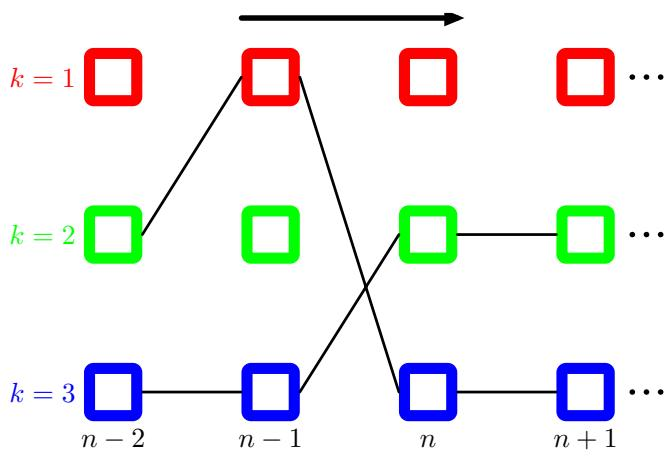
\includegraphics[keepaspectratio,alt={image}]{images/5b320e53d0f84f93813f8b459fc4dcd9d9f2d7f7da3cd0daeda372c742e0e1d8.jpg}}

corresponding to the graph shown in Figure 8.38. Suppose we take node
\(x _ { N }\) to be the root node. Then in the first phase, we propagate
messages from the leaf node \(x _ { 1 }\) to the root node using

\[
\begin{array}{r c l} \mu_ {x _ {n} \to f _ {n, n + 1}} (x _ {n}) & = & \mu_ {f _ {n - 1, n} \to x _ {n}} (x _ {n}) \\ \mu_ {f _ {n - 1, n} \to x _ {n}} (x _ {n}) & = & \max _ {x _ {n - 1}} \left[ \ln f _ {n - 1, n} (x _ {n - 1}, x _ {n}) + \mu_ {x _ {n - 1} \to f n - 1, n} (x _ {n}) \right] \end{array}
\]

which follow from applying (8.94) and (8.93) to this particular graph.
The initial message sent from the leaf node is simply

\[
\mu_ {x _ {1} \rightarrow f _ {1, 2}} (x _ {1}) = 0.\tag{8.99}
\]

The most probable value for \(x _ { N }\) is then given by

\[
x _ {N} ^ {\max} = \underset {x _ {N}} {\arg \max} \left[ \mu_ {f _ {N - 1, N} \to x _ {N}} (x _ {N}) \right].\tag{8.100}
\]

Now we need to determine the states of the previous variables that
correspond to the same maximizing configuration. This can be done by
keeping track of which values of the variables gave rise to the maximum
state of each variable, in other words by storing quantities given by

\[
\phi (x _ {n}) = \underset {x _ {n - 1}} {\arg \max} \left[ \ln f _ {n - 1, n} (x _ {n - 1}, x _ {n}) + \mu_ {x _ {n - 1} \to f n - 1, n} (x _ {n}) \right].\tag{8.101}
\]

To understand better what is happening, it is helpful to represent the
chain of variables in terms of a lattice or trellis diagram as shown in
Figure 8.53. Note that this is not a probabilistic graphical model
because the nodes represent individual states of variables, while each
variable corresponds to a column of such states in the diagram. For each
state of a given variable, there is a unique state of the previous
variable that maximizes the probability (ties are broken either
systematically or at random), corresponding to the function
\(\phi ( x _ { n } )\) given by (8.101), and this is indicated by the
lines connecting the nodes. Once we know the most probable value of the
final node \(x _ { N }\) , we can then simply follow the link back to
find the most probable state of node \(x _ { N - 1 }\) and so on back to
the initial node \(x _ { 1 }\) . This corresponds to propagating a
message back down the chain using

\[
x _ {n - 1} ^ {\mathrm{max}} = \phi (x _ {n} ^ {\mathrm{max}})\tag{8.102}
\]

and is known as back-tracking. Note that there could be several values
of \(x _ { n - 1 }\) all of which give the maximum value in (8.101).
Provided we chose one of these values when we do the back-tracking, we
are assured of a globally consistent maximizing configuration.

In Figure 8.53, we have indicated two paths, each of which we shall
suppose corresponds to a global maximum of the joint probability
distribution. If \(k = 2\) and \(k = 3\) each represent possible values
of \(x _ { N } ^ { \mathrm { m a x } }\) , then starting from either
state and tracing back along the black lines, which corresponds to
iterating (8.102), we obtain a valid global maximum configuration. Note
that if we had run a forward pass of max-sum message passing followed by
a backward pass and then applied (8.98) at each node separately, we
could end up selecting some states from one path and some from the other
path, giving an overall configuration that is not a global maximizer. We
see that it is necessary instead to keep track of the maximizing states
during the forward pass using the functions \(\phi ( x _ { n } )\) and
then use back-tracking to find a consistent solution.

The extension to a general tree-structured factor graph should now be
clear. If a message is sent from a factor node \(f\) to a variable node
\(x ,\) a maximization is performed over all other variable nodes
\(x _ { 1 } , \ldots , x _ { M }\) that are neighbours of that factor
node, using (8.93). When we perform this maximization, we keep a record
of which values of the variables \(x _ { 1 } , \ldots , x _ { M }\) gave
rise to the maximum. Then in the back-tracking step, having found
\(x ^ { \mathrm { m a x } }\) , we can then use these stored values to
assign consistent maximizing states
\(x _ { 1 } ^ { \mathrm { m a x } } , \ldots , x _ { M } ^ { \mathrm { m a x } }\)
. The max-sum algorithm, with back-tracking, gives an exact maximizing
configuration for the variables provided the factor graph is a tree. An
important application of this technique is for finding the most probable
sequence of hidden states in a hidden Markov model, in which case it is
known as the Viterbi algorithm.

As with the sum-product algorithm, the inclusion of evidence in the form
of observed variables is straightforward. The observed variables are
clamped to their observed values, and the maximization is performed over
the remaining hidden variables. This can be shown formally by including
identity functions for the observed variables into the factor functions,
as we did for the sum-product algorithm.

It is interesting to compare max-sum with the iterated conditional modes
(ICM) algorithm described on page 389. Each step in ICM is
computationally simpler because the `messages' that are passed from one
node to the next comprise a single value consisting of the new state of
the node for which the conditional distribution is maximized. The
max-sum algorithm is more complex because the messages are functions of
node variables x and hence comprise a set of K values for each possible
state of x. Unlike max-sum, however, ICM is not guaranteed to find a
global maximum even for tree-structured graphs.

\subsection{8.4.6 Exact inference in general
graphs}\label{exact-inference-in-general-graphs}

The sum-product and max-sum algorithms provide efficient and exact
solutions to inference problems in tree-structured graphs. For many
practical applications, however, we have to deal with graphs having
loops.

The message passing framework can be generalized to arbitrary graph
topologies, giving an exact inference procedure known as the junction
tree algorithm (Lauritzen and Spiegelhalter, 1988; Jordan, 2007). Here
we give a brief outline of the key steps involved. This is not intended
to convey a detailed understanding of the algorithm, but rather to give
a flavour of the various stages involved. If the starting point is a
directed graph, it is first converted to an undirected graph by
moralization, whereas if starting from an undirected graph this step is
not required. Next the graph is triangulated, which involves finding
chord-less cycles containing four or more nodes and adding extra links
to eliminate such chord-less cycles. For instance, in the graph in
Figure 8.36, the cycle \(A { - } C { - } B { - } D { - } A\) is
chord-less a link could be added between A and B or alternatively
between C and D. Note that the joint distribution for the resulting
triangulated graph is still defined by a product of the same potential
functions, but these are now considered to be functions over expanded
sets of variables. Next the triangulated graph is used to construct a
new tree-structured undirected graph called a join tree, whose nodes
correspond to the maximal cliques of the triangulated graph, and whose
links connect pairs of cliques that have variables in common. The
selection of which pairs of cliques to connect in this way is important
and is done so as to give a maximal spanning tree defined as follows. Of
all possible trees that link up the cliques, the one that is chosen is
one for which the weight of the tree is largest, where the weight for a
link is the number of nodes shared by the two cliques it connects, and
the weight for the tree is the sum of the weights for the links. If the
tree is condensed, so that any clique that is a subset of another clique
is absorbed into the larger clique, this gives ajunction tree. As a
consequence of the triangulation step, the resulting tree satisfies the
running intersection property, which means that if a variable is
contained in two cliques, then it must also be contained in every clique
on the path that connects them. This ensures that inference about
variables will be consistent across the graph. Finally, a two-stage
message passing algorithm, essentially equivalent to the sum-product
algorithm, can now be applied to this junction tree in order to find
marginals and conditionals. Although the junction tree algorithm sounds
complicated, at its heart is the simple idea that we have used already
of exploiting the factorization properties of the distribution to allow
sums and products to be interchanged so that partial summations can be
performed, thereby avoiding having to work directly with the joint
distribution. The role of the junction tree is to provide a precise and
efficient way to organize these computations. It is worth emphasizing
that this is achieved using purely graphical operations!

The junction tree is exact for arbitrary graphs and is efficient in the
sense that for a given graph there does not in general exist a
computationally cheaper approach. Unfortunately, the algorithm must work
with the joint distributions within each node (each of which corresponds
to a clique of the triangulated graph) and so the computational cost of
the algorithm is determined by the number of variables in the largest
clique and will grow exponentially with this number in the case of
discrete variables. An important concept is the treewidth of a graph
(Bodlaender, 1993), which is defined in terms of the number of variables
in the largest clique. In fact, it is defined to be as one less than the
size of the largest clique, to ensure that a tree has a treewidth of 1.
Because there in general there can be multiple different junction trees
that can be constructed from a given starting graph, the treewidth is
defined by the junction tree for which the largest clique has the fewest
variables. If the treewidth of the original graph is high, the junction
tree algorithm becomes impractical.

\subsection{8.4.7 Loopy belief
propagation}\label{loopy-belief-propagation}

For many problems of practical interest, it will not be feasible to use
exact inference, and so we need to exploit effective approximation
methods. An important class of such approximations, that can broadly be
called variational methods, will be discussed in detail in Chapter 10.
Complementing these deterministic approaches is a wide range of sampling
methods, also called Monte Carlo methods, that are based on stochastic
numerical sampling from distributions and that will be discussed at
length in Chapter 11.

Here we consider one simple approach to approximate inference in graphs
with loops, which builds directly on the previous discussion of exact
inference in trees. The idea is simply to apply the sum-product
algorithm even though there is no guarantee that it will yield good
results. This approach is known as loopy belief propagation (Frey and
MacKay, 1998) and is possible because the message passing rules (8.66)
and (8.69) for the sum-product algorithm are purely local. However,
because the graph now has cycles, information can flow many times around
the graph. For some models, the algorithm will converge, whereas for
others it will not.

In order to apply this approach, we need to define a message passing
schedule. Let us assume that one message is passed at a time on any
given link and in any given direction. Each message sent from a node
replaces any previous message sent in the same direction across the same
link and will itself be a function only of the most recent messages
received by that node at previous steps of the algorithm.

We have seen that a message can only be sent across a link from a node
when all other messages have been received by that node across its other
links. Because there are loops in the graph, this raises the problem of
how to initiate the message passing algorithm. To resolve this, we
suppose that an initial message given by the unit function has been
passed across every link in each direction. Every node is then in a
position to send a message.

There are now many possible ways to organize the message passing
schedule. For example, the flooding schedule simultaneously passes a
message across every link in both directions at each time step, whereas
schedules that pass one message at a time are called serial schedules.

Following Kschischnang et al.~(2001), we will say that a (variable or
factor) node a has a message pending on its link to a node b if node a
has received any message on any of its other links since the last time
it send a message to b. Thus, when a node receives a message on one of
its links, this creates pending messages on all of its other links. Only
pending messages need to be transmitted because other messages would
simply duplicate the previous message on the same link. For graphs that
have a tree structure, any schedule that sends only pending messages
will eventually terminate once a message has passed in each direction
across every link. At this point, there are no pending messages, and the
product of the received messages at every variable give the exact
marginal. In graphs having loops, however, the algorithm may never
terminate because there might always be pending messages, although in
practice it is generally found to converge within a reasonable time for
most applications. Once the algorithm has converged, or once it has been
stopped if convergence is not observed, the (approximate) local
marginals can be computed using the product of the most recently
received incoming messages to each variable node or factor node on every
link.

In some applications, the loopy belief propagation algorithm can give
poor results, whereas in other applications it has proven to be very
effective. In particular, state-of-the-art algorithms for decoding
certain kinds of error-correcting codes are equivalent to loopy belief
propagation (Gallager, 1963; Berrou et al., 1993; McEliece et al., 1998;
MacKay and Neal, 1999; Frey, 1998).

\subsection{8.4.8 Learning the graph
structure}\label{learning-the-graph-structure}

In our discussion of inference in graphical models, we have assumed that
the structure of the graph is known and fixed. However, there is also
interest in going beyond the inference problem and learning the graph
structure itself from data (Friedman and Koller, 2003). This requires
that we define a space of possible structures as well as a measure that
can be used to score each structure.

From a Bayesian viewpoint, we would ideally like to compute a posterior
distribution over graph structures and to make predictions by averaging
with respect to this distribution. If we have a prior \(p ( m )\) over
graphs indexed by m, then the posterior distribution is given by

\[
p (m | \mathcal {D}) \propto p (m) p (\mathcal {D} | m)\tag{8.103}
\]

where is the observed data set. The model evidence
\(p ( \mathcal { D } | m )\) then provides the score for each model.
However, evaluation of the evidence involves marginalization over the
latent variables and presents a challenging computational problem for
many models.

Exploring the space of structures can also be problematic. Because the
number of different graph structures grows exponentially with the number
of nodes, it is often necessary to resort to heuristics to find good
candidates.

\subsection{Exercises}\label{exercises}

8.1 () www By marginalizing out the variables in order, show that the
representation (8.5) for the joint distribution of a directed graph is
correctly normalized, provided each of the conditional distributions is
normalized.

8.2 () www Show that the property of there being no directed cycles in a
directed graph follows from the statement that there exists an ordered
numbering of the nodes such that for each node there are no links going
to a lower-numbered node.

Table 8.2 The joint distribution over three binary variables.

{\def\LTcaptype{none} % do not increment counter
\begin{longtable}[]{@{}|l|l|l|l|@{}}
\toprule\noalign{}
\endhead
\bottomrule\noalign{}
\endlastfoot
\hline
a & b & c & p(a,b,c) \\
\hline
0 & 0 & 0 & 0.192 \\
\hline
0 & 0 & 1 & 0.144 \\
\hline
0 & 1 & 0 & 0.048 \\
\hline
0 & 1 & 1 & 0.216 \\
\hline
1 & 0 & 0 & 0.192 \\
\hline
1 & 0 & 1 & 0.064 \\
\hline
1 & 1 & 0 & 0.048 \\
\hline
1 & 1 & 1 & 0.096 \\
\hline
\end{longtable}
}

8.3 ( ) Consider three binary variables \(a , b , c \in \{ 0 , 1 \}\)
having the joint distribution given in Table 8.2. Show by direct
evaluation that this distribution has the property that a and b are
marginally dependent, so that \(p ( a , b ) \neq p ( a ) p ( b )\) , but
that they become independent when conditioned on \(c ,\) so that
\(p ( a , b | c ) \ : = \ : p ( a | c ) p ( b | c )\) for both \(c = 0\)
and \(c = 1\)

8.4 ( ) Evaluate the distributions \(p ( a ) , p ( b | c )\) , and
\(p ( c | a )\) corresponding to the joint distribution given in Table
8.2. Hence show by direct evaluation that \(p ( a , b , c ) =\)
\(p ( a ) p ( c | a ) p ( b | c )\) . Draw the corresponding directed
graph.

8.5 () www Draw a directed probabilistic graphical model corresponding
to the relevance vector machine described by (7.79) and (7.80).

8.6 () For the model shown in Figure 8.13, we have seen that the number
of parameters required to specify the conditional distribution
\(p ( y | x _ { 1 } , \dots , x _ { M } )\) , where
\(x _ { i } \in \{ 0 , 1 \}\) , could be reduced from \(2 ^ { M }\) to
\(M + 1\) by making use of the logistic sigmoid representation (8.10).
An alternative representation (Pearl, 1988) is given by

\[
p (y = 1 \mid x _ {1}, \dots , x _ {M}) = 1 - (1 - \mu_ {0}) \prod_ {i = 1} ^ {M} (1 - \mu_ {i}) ^ {x _ {i}}\tag{8.104}
\]

where the parameters \(\mu _ { i }\) represent the probabilities
\(p ( x _ { i } = 1 )\) , and \(\mu _ { 0 }\) is an additional
parameters satisfying \(0 \leqslant \mu _ { 0 } \leqslant 1\) . The
conditional distribution \(_ { ( 8 . 1 0 4 ) }\) is known as the
noisy-OR. Show that this can be interpreted as a `soft' (probabilistic)
form of the logical OR function (i.e., the function that gives \(y = 1\)
whenever at least one of the \(x _ { i } = 1 )\) . Discuss the
interpretation of \(\mu _ { 0 }\)

8.7 ( ) Using the recursion relations (8.15) and (8.16), show that the
mean and covariance of the joint distribution for the graph shown in
Figure 8.14 are given by (8.17) and (8.18), respectively.

8.8 () www Show that \(a \perp \perp b , c \parallel\) d implies
\(a \perp \perp b \mid d .\)

8.9 () www Using the d-separation criterion, show that the conditional
distribution for a node x in a directed graph, conditioned on all of the
nodes in the Markov blanket, is independent of the remaining variables
in the graph.

Figure 8.54 Example of a graphical model used to explore the conditional
independence properties of the head-to-head path \(a { - } c { - } b\)
when a descendant of \(^ { c , }\) namely the node \(d ,\) is observed.

\pandocbounded{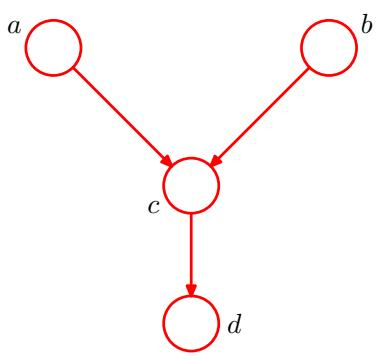
\includegraphics[keepaspectratio,alt={image}]{images/1bf32998f7437c021861b596a8d178f94e48b85ffc2b985e5bb80a8f31992776.jpg}}

8.10 () Consider the directed graph shown in Figure 8.54 in which none
of the variables is observed. Show that
\(a \perp \perp b \mid \emptyset\) . Suppose we now observe the variable
d.~Show that in general \(a \not \perp b \mid d .\)

8.11 ( ) Consider the example of the car fuel system shown in Figure
8.21, and suppose that instead of observing the state of the fuel gauge
G directly, the gauge is seen by the driver D who reports to us the
reading on the gauge. This report is either that the gauge shows full
\(D = 1\) or that it shows empty \(D = 0\) . Our driver is a bit
unreliable, as expressed through the following probabilities

\[
p (D = 1 | G = 1) = 0. 9\tag{8.105}
\]

\[
p (D = 0 | G = 0) = 0. 9.\tag{8.106}
\]

Suppose that the driver tells us that the fuel gauge shows empty, in
other words that we observe \(D = 0\) . Evaluate the probability that
the tank is empty given only this observation. Similarly, evaluate the
corresponding probability given also the observation that the battery is
flat, and note that this second probability is lower. Discuss the
intuition behind this result, and relate the result to Figure 8.54.

8.12 () www Show that there are \(2 ^ { M ( M - 1 ) / 2 }\) distinct
undirected graphs over a set of M distinct random variables. Draw the 8
possibilities for the case of \(M = 3\)

8.13 () Consider the use of iterated conditional modes (ICM) to minimize
the energy function given by (8.42). Write down an expression for the
difference in the values of the energy associated with the two states of
a particular variable \(x _ { j }\) , with all other variables held
fixed, and show that it depends only on quantities that are local to
\(x _ { j }\) in the graph.

8.14 () Consider a particular case of the energy function given by
(8.42) in which the coefficients \(\beta = h = 0\) . Show that the most
probable configuration of the latent variables is given by
\(x _ { i } = y _ { i }\) for all i.

8.15 ( ) www Show that the joint distribution
\(p ( x _ { n - 1 } , x _ { n } )\) for two neighbouring nodes in the
graph shown in Figure 8.38 is given by an expression of the form (8.58).

8.16 ( ) Consider the inference problem of evaluating
\(p ( \mathbf { x } _ { n } | \mathbf { x } _ { N } )\) for the graph
shown in Figure 8.38, for all nodes \(n \in \{ 1 , \ldots , N - 1 \}\) .
Show that the message passing algorithm discussed in Section 8.4.1 can
be used to solve this efficiently, and discuss which messages are
modified and in what way.

8.17 ( ) Consider a graph of the form shown in Figure 8.38 having
\(N = 5\) nodes, in which nodes \(x _ { 3 }\) and \(x _ { 5 }\) are
observed. Use d-separation to show that
\(x _ { 2 } \perp \perp x _ { 5 } \mid x _ { 3 }\) Show that if the
message passing algorithm of Section 8.4.1 is applied to the evaluation
of \(p ( x _ { 2 } | x _ { 3 } , x _ { 5 } )\) , the result will be
independent of the value of \(x _ { 5 }\)

8.18 ( ) www Show that a distribution represented by a directed tree can
trivially be written as an equivalent distribution over the
corresponding undirected tree. Also show that a distribution expressed
as an undirected tree can, by suitable normalization of the clique
potentials, be written as a directed tree. Calculate the number of
distinct directed trees that can be constructed from a given undirected
tree.

8.19 ( ) Apply the sum-product algorithm derived in Section 8.4.4 to the
chain-ofnodes model discussed in Section 8.4.1 and show that the results
(8.54), (8.55), and (8.57) are recovered as a special case.

8.20 () www Consider the message passing protocol for the sum-product
algorithm on a tree-structured factor graph in which messages are first
propagated from the leaves to an arbitrarily chosen root node and then
from the root node out to the leaves. Use proof by induction to show
that the messages can be passed in such an order that at every step,
each node that must send a message has received all of the incoming
messages necessary to construct its outgoing messages.

8.21 ( ) www Show that the marginal distributions
\(p ( \mathbf { x } _ { s } )\) over the sets of variables
\(\mathbf { x } _ { s }\) associated with each of the factors
\(f _ { x } ( \mathbf { x } _ { s } )\) in a factor graph can be found
by first running the sum-product message passing algorithm and then
evaluating the required marginals using (8.72).

8.22 () Consider a tree-structured factor graph, in which a given subset
of the variable nodes form a connected subgraph (i.e., any variable node
of the subset is connected to at least one of the other variable nodes
via a single factor node). Show how the sum-product algorithm can be
used to compute the marginal distribution over that subset.

8.23 ( ) www In Section 8.4.4, we showed that the marginal distribution
\(p ( x _ { i } )\) for a variable node \(x _ { i }\) in a factor graph
is given by the product of the messages arriving at this node from
neighbouring factor nodes in the form (8.63). Show that the marginal
\(p ( x _ { i } )\) can also be written as the product of the incoming
message along any one of the links with the outgoing message along the
same link.

8.24 ( ) Show that the marginal distribution for the variables
\(\mathbf { x } _ { s }\) in a factor
\(f _ { s } ( \mathbf { x } _ { s } )\) in a tree-structured factor
graph, after running the sum-product message passing algorithm, can be
written as the product of the message arriving at the factor node along
all its links, times the local factor \(f ( \mathbf { x } _ { s } )\) ,
in the form (8.72).

8.25 \(( \star \star )\) In (8.86), we verified that the sum-product
algorithm run on the graph in Figure 8.51 with node \(x _ { 3 }\)
designated as the root node gives the correct marginal for \(x _ { 2 }\)
. Show that the correct marginals are obtained also for \(x _ { 1 }\)
and \(x _ { 3 }\) . Similarly, show that the use of the result (8.72)
after running the sum-product algorithm on this graph gives the correct
joint distribution for \(x _ { 1 } , x _ { 2 }\)

8.26 () Consider a tree-structured factor graph over discrete variables,
and suppose we wish to evaluate the joint distribution
\(p ( x _ { a } , x _ { b } )\) associated with two variables
\(x _ { a }\) and \(x _ { b }\) that do not belong to a common factor.
Define a procedure for using the sumproduct algorithm to evaluate this
joint distribution in which one of the variables is successively clamped
to each of its allowed values.

8.27 ( ) Consider two discrete variables x and y each having three
possible states, for example \(x , y \in \{ 0 , 1 , 2 \}\) . Construct a
joint distribution \(p ( x , y )\) over these variables having the
property that the value \(\widehat { x }\) that maximizes the marginal
\(p ( x )\) , along with the value \(\widehat { y }\) that maximizes the
marginal \(p ( y )\) , together have probability zero under the joint
distribution, so that \(p ( \widehat { x } , \widehat { y } ) = 0\)

8.28 ( ) www The concept of a pending message in the sum-product
algorithm for a factor graph was defined in Section 8.4.7. Show that if
the graph has one or more cycles, there will always be at least one
pending message irrespective of how long the algorithm runs.

8.29 ( ) www Show that if the sum-product algorithm is run on a factor
graph with a tree structure (no loops), then after a finite number of
messages have been sent, there will be no pending messages.

\section{Mixture Models and EM}\label{mixture-models-and-em}

\pandocbounded{
\includegraphics[keepaspectratio,alt={image}]{images/6c368ae6dca55b1d809e9c5ad1b184604187377c63fe40fc04ca37329f1ec23f.jpg}}

If we define a joint distribution over observed and latent variables,
the corresponding distribution of the observed variables alone is
obtained by marginalization. This allows relatively complex marginal
distributions over observed variables to be expressed in terms of more
tractable joint distributions over the expanded space of observed and
latent variables. The introduction of latent variables thereby allows
complicated distributions to be formed from simpler components. In this
chapter, we shall see that mixture distributions, such as the Gaussian
mixture discussed in Section 2.3.9, can be interpreted in terms of
discrete latent variables. Continuous latent variables will form the
subject of Chapter 12.

As well as providing a framework for building more complex probability
distributions, mixture models can also be used to cluster data. We
therefore begin our discussion of mixture distributions by considering
the problem of finding clusters in a set of data points, which we
approach first using a nonprobabilistic technique called the K-means
algorithm (Lloyd, 1982). Then we introduce the latent variable view of
mixture distributions in which the discrete latent variables can be
interpreted as defining assignments of data points to specific
components of the mixture. A general technique for finding maximum
likelihood estimators in latent variable models is the
expectation-maximization (EM) algorithm. We first of all use the
Gaussian mixture distribution to motivate the EM algorithm in a fairly
informal way, and then we give a more careful treatment based on the
latent variable viewpoint. We shall see that the K-means algorithm
corresponds to a particular nonprobabilistic limit of EM applied to
mixtures of Gaussians. Finally, we discuss EM in some generality.

Gaussian mixture models are widely used in data mining, pattern
recognition, machine learning, and statistical analysis. In many
applications, their parameters are determined by maximum likelihood,
typically using the EM algorithm. However, as we shall see there are
some significant limitations to the maximum likelihood approach, and in
Chapter 10 we shall show that an elegant Bayesian treatment can be given
using the framework of variational inference. This requires little
additional computation compared with EM, and it resolves the principal
difficulties of maximum likelihood while also allowing the number of
components in the mixture to be inferred automatically from the data.

\subsection{9.1. K-means Clustering}\label{k-means-clustering}

We begin by considering the problem of identifying groups, or clusters,
of data points in a multidimensional space. Suppose we have a data set
\(\left\{ \mathbf { x } _ { 1 } , \ldots , \mathbf { x } _ { N } \right\}\)
consisting of N observations of a random D-dimensional Euclidean
variable x. Our goal is to partition the data set into some number K of
clusters, where we shall suppose for the moment that the value of K is
given. Intuitively, we might think of a cluster as comprising a group of
data points whose inter-point distances are small compared with the
distances to points outside of the cluster. We can formalize this notion
by first introducing a set of D-dimensional vectors
\(\pmb { \mu } _ { k }\) , where \(k = 1 , \ldots , K\) , in which
\(\pmb { \mu } _ { k }\) is a prototype associated with the
\(k ^ { \mathrm { t h } }\) cluster. As we shall see shortly, we can
think of the \(\pmb { \mu } _ { k }\) as representing the centres of the
clusters. Our goal is then to find an assignment of data points to
clusters, as well as a set of vectors \(\{ \mu _ { k } \}\) , such that
the sum of the squares of the distances of each data point to its
closest vector \(\mu _ { k }\) , is a minimum.

It is convenient at this point to define some notation to describe the
assignment of data points to clusters. For each data point
\(\mathbf { x } _ { n } .\) , we introduce a corresponding set of binary
indicator variables \(r _ { n k } \in \{ 0 , 1 \}\) , where
\(k = 1 , \ldots , K\) describing which of the K clusters the data point
\({ \bf x } _ { n }\) is assigned to, so that if data point
\({ \bf x } _ { n }\) is assigned to cluster k then \(r _ { n k } = 1\)
, and \(r _ { n j } = 0\) for \(j \neq k\) . This is known as the 1-of-K
coding scheme. We can then define an objective function, sometimes
called a distortion measure, given by

\[
J = \sum_ {n = 1} ^ {N} \sum_ {k = 1} ^ {K} r _ {n k} \| \mathbf {x} _ {n} - \pmb {\mu} _ {k} \| ^ {2}\tag{9.1}
\]

which represents the sum of the squares of the distances of each data
point to its assigned vector \(\pmb { \mu } _ { k }\) . Our goal is to
find values for the \(\{ r _ { n k } \}\) and the \(\{ \mu _ { k } \}\)
so as to minimize J. We can do this through an iterative procedure in
which each iteration involves two successive steps corresponding to
successive optimizations with respect to the \(r _ { n k }\) and the
\(\mu _ { k }\) . First we choose some initial values for the
\(\pmb { \mu } _ { k }\) . Then in the first phase we minimize J with
respect to the \(r _ { n k }\) , keeping the \(\mu _ { k }\) fixed. In
the second phase we minimize J with respect to the
\(\pmb { \mu } _ { k }\) , keeping \(r _ { n k }\) fixed. This two-stage
optimization is then repeated until convergence. We shall see that these
two stages of updating \(r _ { n k }\) and updating
\(\pmb { \mu } _ { k }\) correspond respectively to the E (expectation)
and M (maximization) steps of the EM algorithm, and to emphasize this we
shall use the terms E step and M step in the context of the K-means
algorithm.

Consider first the determination of the \(r _ { n k }\) . Because J in
(9.1) is a linear function of \(r _ { n k }\) , this optimization can be
performed easily to give a closed form solution. The terms involving
different n are independent and so we can optimize for each n separately
by choosing \(r _ { n k }\) to be 1 for whichever value of k gives the
minimum value of
\(\| \mathbf { x } _ { n } - \pmb { \mu } _ { k } \| ^ { 2 }\) . In
other words, we simply assign the \(n ^ { \mathrm { t h } }\) data point
to the closest cluster centre. More formally, this can be expressed as

\[
r _ {n k} = \left\{ \begin{array}{l l} 1 & \text { if } k = \arg \min _ {j} \| \mathbf {x} _ {n} - \boldsymbol {\mu} _ {j} \| ^ {2} \\ 0 & \text { otherwise. } \end{array} \right.\tag{9.2}
\]

Now consider the optimization of the \(\pmb { \mu } _ { k }\) with the
\(r _ { n k }\) held fixed. The objective function J is a quadratic
function of \(\pmb { \mu } _ { k }\) , and it can be minimized by
setting its derivative with respect to \(\pmb { \mu } _ { k }\) to zero
giving

\[
2 \sum_ {n = 1} ^ {N} r _ {n k} (\mathbf {x} _ {n} - \boldsymbol {\mu} _ {k}) = 0\tag{9.3}
\]

which we can easily solve for \(\mu _ { k }\) to give

\[
\pmb {\mu} _ {k} = \frac {\sum_ {n} r _ {n k} \mathbf {x} _ {n}}{\sum_ {n} r _ {n k}}.\tag{9.4}
\]

The denominator in this expression is equal to the number of points
assigned to cluster \(k ,\) and so this result has a simple
interpretation, namely set \(\mu _ { k }\) equal to the mean of all of
the data points \({ \bf x } _ { n }\) assigned to cluster k. For this
reason, the procedure is known as the K-means algorithm.

The two phases of re-assigning data points to clusters and re-computing
the cluster means are repeated in turn until there is no further change
in the assignments (or until some maximum number of iterations is
exceeded). Because each phase reduces the value of the objective
function J, convergence of the algorithm is assured. However, it may
converge to a local rather than global minimum of J. The convergence
properties of the K-means algorithm were studied by MacQueen (1967).

The K-means algorithm is illustrated using the Old Faithful data set in
Figure 9.1. For the purposes of this example, we have made a linear
re-scaling of the data, known as standardizing, such that each of the
variables has zero mean and unit standard deviation. For this example,
we have chosen \(K = 2\) , and so in this case, the assignment of each
data point to the nearest cluster centre is equivalent to a
classification of the data points according to which side they lie of
the perpendicular bisector of the two cluster centres. A plot of the
cost function J given by (9.1) for the Old Faithful example is shown in
Figure 9.2.

\pandocbounded{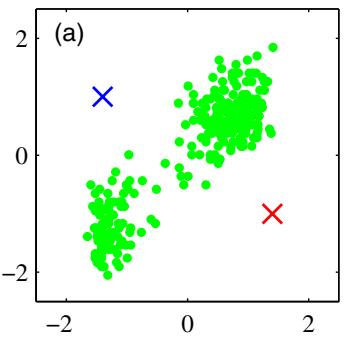
\includegraphics[keepaspectratio,alt={image}]{images/87f8b82d31072e6160cf80baffa345bc02b85adb72842ac061f6e51d28af24c0.jpg}}

\pandocbounded{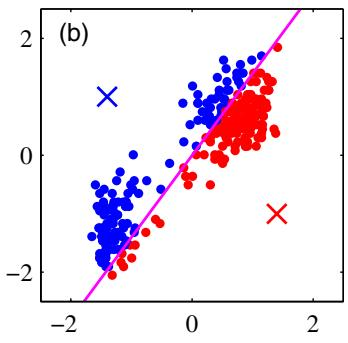
\includegraphics[keepaspectratio,alt={image}]{images/18d17755b5aea4bf6d03376a875096ca9838d537546b93aa6d0794d7e5b8b7bd.jpg}}

\pandocbounded{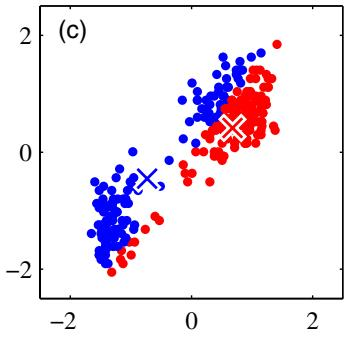
\includegraphics[keepaspectratio,alt={image}]{images/90610fed0dfce0d22388c8f2894753f715021214d8de1820f6640e009066cb2a.jpg}}

\pandocbounded{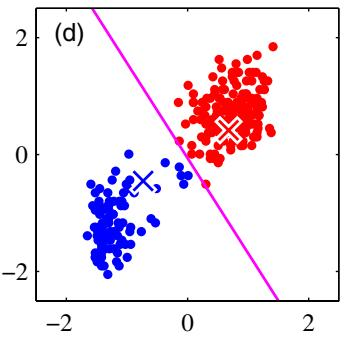
\includegraphics[keepaspectratio,alt={image}]{images/fd36170c13d446e0a13cb7db1cdb4b3609f2ff5d12115146cea669d98ce9c12b.jpg}}

\pandocbounded{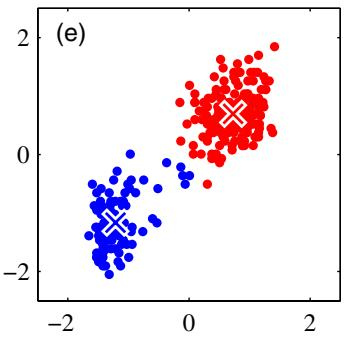
\includegraphics[keepaspectratio,alt={image}]{images/075205e7753842645e3d5228c2ee1c3ff7434d24e6ce0efe675d0fb69869eb09.jpg}}

\pandocbounded{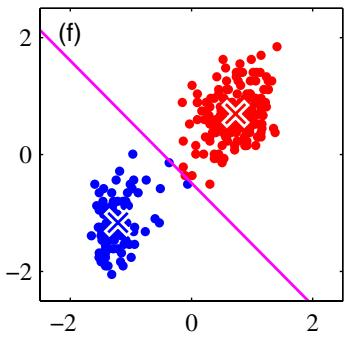
\includegraphics[keepaspectratio,alt={image}]{images/5fc7c085a5f32678c3ac21e91e9369f521f5635ab6db3b80c82abcc5ce35630b.jpg}}

\pandocbounded{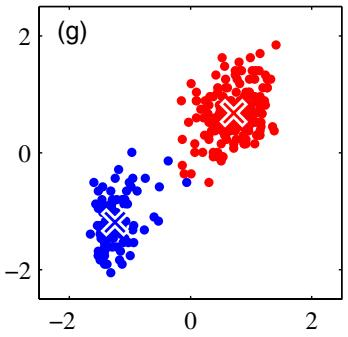
\includegraphics[keepaspectratio,alt={image}]{images/ca87ac02ff95cdeae964d336233aeba6530847449f74f4c9f32761488f1c7978.jpg}}

\pandocbounded{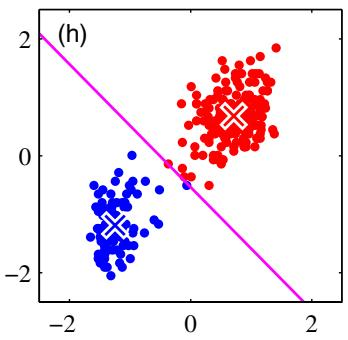
\includegraphics[keepaspectratio,alt={image}]{images/c47ca54eb7e55f10b25103da097cd786e695ca505fda69aea3dac69eff530bdc.jpg}}

\pandocbounded{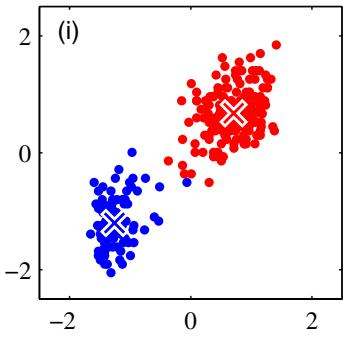
\includegraphics[keepaspectratio,alt={image}]{images/1868146e82a96d9a705c40396994c5cd8cd8a657bbcd02408073fe506aca86c7.jpg}}

Figure 9.1 Illustration of the K-means algorithm using the re-scaled Old
Faithful data set. (a) Green points denote the data set in a
two-dimensional Euclidean space. The initial choices for centres
\(\pmb { \mu } _ { 1 }\) and \(\mu _ { 2 }\) are shown by the red and
blue crosses, respectively. (b) In the initial E step, each data point
is assigned either to the red cluster or to the blue cluster, according
to which cluster centre is nearer. This is equivalent to classifying the
points according to which side of the perpendicular bisector of the two
cluster centres, shown by the magenta line, they lie on. (c) In the
subsequent M step, each cluster centre is re-computed to be the mean of
the points assigned to the corresponding cluster. (d)--(i) show
successive E and M steps through to final convergence of the algorithm.

Plot of the cost function J given by (9.1) after each E step (blue
points) and M step (red points) of the Kmeans algorithm for the example
shown in Figure 9.1. The algorithm has converged after the third M step,
and the final EM cycle produces no changes in either the assignments or
the prototype vectors.

\pandocbounded{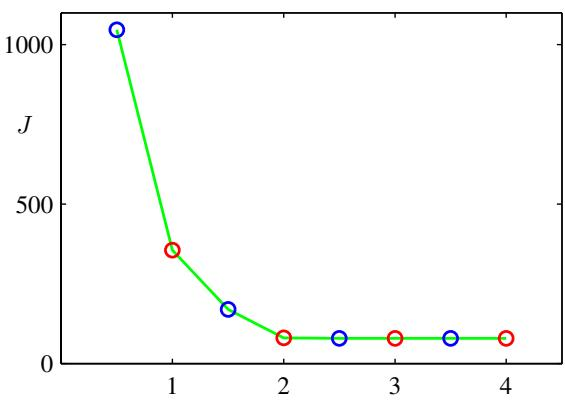
\includegraphics[keepaspectratio,alt={image}]{images/e5a51ec29e7e0bd6d4e39df4a9a1c1cde47006f54904324660899cbe4c0cfe93.jpg}}

Note that we have deliberately chosen poor initial values for the
cluster centres so that the algorithm takes several steps before
convergence. In practice, a better initialization procedure would be to
choose the cluster centres \(\pmb { \mu } _ { k }\) to be equal to a
random subset of K data points. It is also worth noting that the K-means
algorithm itself is often used to initialize the parameters in a
Gaussian mixture model before applying the EM algorithm.

A direct implementation of the K-means algorithm as discussed here can
be relatively slow, because in each E step it is necessary to compute
the Euclidean distance between every prototype vector and every data
point. Various schemes have been proposed for speeding up the K-means
algorithm, some of which are based on precomputing a data structure such
as a tree such that nearby points are in the same subtree
(Ramasubramanian and Paliwal, 1990; Moore, 2000). Other approaches make
use of the triangle inequality for distances, thereby avoiding
unnecessary distance calculations (Hodgson, 1998; Elkan, 2003).

So far, we have considered a batch version of K-means in which the whole
data set is used together to update the prototype vectors. We can also
derive an on-line stochastic algorithm (MacQueen, 1967) by applying the
Robbins-Monro procedure to the problem of finding the roots of the
regression function given by the derivatives of J in (9.1) with respect
to \(\mu _ { k }\) . This leads to a sequential update in which, for
each data point \({ \bf x } _ { n }\) in turn, we update the nearest
prototype \(\mu _ { k }\) using

\[
\pmb {\mu} _ {k} ^ {\mathrm{new}} = \pmb {\mu} _ {k} ^ {\mathrm{old}} + \eta_ {n} (\mathbf {x} _ {n} - \pmb {\mu} _ {k} ^ {\mathrm{old}})\tag{9.5}
\]

where \(\eta _ { n }\) is the learning rate parameter, which is
typically made to decrease monotonically as more data points are
considered.

The K-means algorithm is based on the use of squared Euclidean distance
as the measure of dissimilarity between a data point and a prototype
vector. Not only does this limit the type of data variables that can be
considered (it would be inappropriate for cases where some or all of the
variables represent categorical labels for instance), but it can also
make the determination of the cluster means nonrobust to outliers. We
can generalize the K-means algorithm by introducing a more general
dissimilarity measure
\(\mathcal { V } ( \mathbf { x } , \mathbf { x } ^ { \prime } )\)
between two vectors x and \(\mathbf { x } ^ { \prime }\) and then
minimizing the following distortion measure

\[
\widetilde {J} = \sum_ {n = 1} ^ {N} \sum_ {k = 1} ^ {K} r _ {n k} \mathcal {V} (\mathbf {x} _ {n}, \pmb {\mu} _ {k})\tag{9.6}
\]

which gives the K-medoids algorithm. The E step again involves, for
given cluster prototypes \(\pmb { \mu } _ { k }\) , assigning each data
point to the cluster for which the dissimilarity to the corresponding
prototype is smallest. The computational cost of this is \(O ( K N )\)
as is the case for the standard K-means algorithm. For a general choice
of dissimilarity measure, the M step is potentially more complex than
for K-means, and so it is common to restrict each cluster prototype to
be equal to one of the data vectors assigned to that cluster, as this
allows the algorithm to be implemented for any choice of dissimilarity
measure \(\mathcal { V } ( \cdot , \cdot )\) so long as it can be
readily evaluated. Thus the M step involves, for each cluster k, a
discrete search over the \(N _ { k }\) points assigned to that cluster,
which requires \(O ( N _ { k } ^ { 2 } )\) evaluations of
\(\mathcal { V } ( \cdot , \cdot )\)

One notable feature of the K-means algorithm is that at each iteration,
every data point is assigned uniquely to one, and only one, of the
clusters. Whereas some data points will be much closer to a particular
centre \(\pmb { \mu } _ { k }\) than to any other centre, there may be
other data points that lie roughly midway between cluster centres. In
the latter case, it is not clear that the hard assignment to the nearest
cluster is the most appropriate. We shall see in the next section that
by adopting a probabilistic approach, we obtain `soft' assignments of
data points to clusters in a way that reflects the level of uncertainty
over the most appropriate assignment. This probabilistic formulation
brings with it numerous benefits.

\subsection{9.1.1 Image segmentation and
compression}\label{image-segmentation-and-compression}

As an illustration of the application of the K-means algorithm, we
consider the related problems of image segmentation and image
compression. The goal of segmentation is to partition an image into
regions each of which has a reasonably homogeneous visual appearance or
which corresponds to objects or parts of objects (Forsyth and Ponce,
2003). Each pixel in an image is a point in a 3-dimensional space
comprising the intensities of the red, blue, and green channels, and our
segmentation algorithm simply treats each pixel in the image as a
separate data point. Note that strictly this space is not Euclidean
because the channel intensities are bounded by the interval {[}0, 1{]}.
Nevertheless, we can apply the K-means algorithm without difficulty. We
illustrate the result of running K-means to convergence, for any
particular value of K, by re-drawing the image replacing each pixel
vector with the \(\{ R , G , B \}\) intensity triplet given by the
centre \(\pmb { \mu } _ { k }\) to which that pixel has been assigned.
Results for various values of K are shown in Figure 9.3. We see that for
a given value of K, the algorithm is representing the image using a
palette of only K colours. It should be emphasized that this use of
K-means is not a particularly sophisticated approach to image
segmentation, not least because it takes no account of the spatial
proximity of different pixels. The image segmentation problem is in
general extremely difficult and remains the subject of active research
and is introduced here simply to illustrate the behaviour of the K-means
algorithm.

\pandocbounded{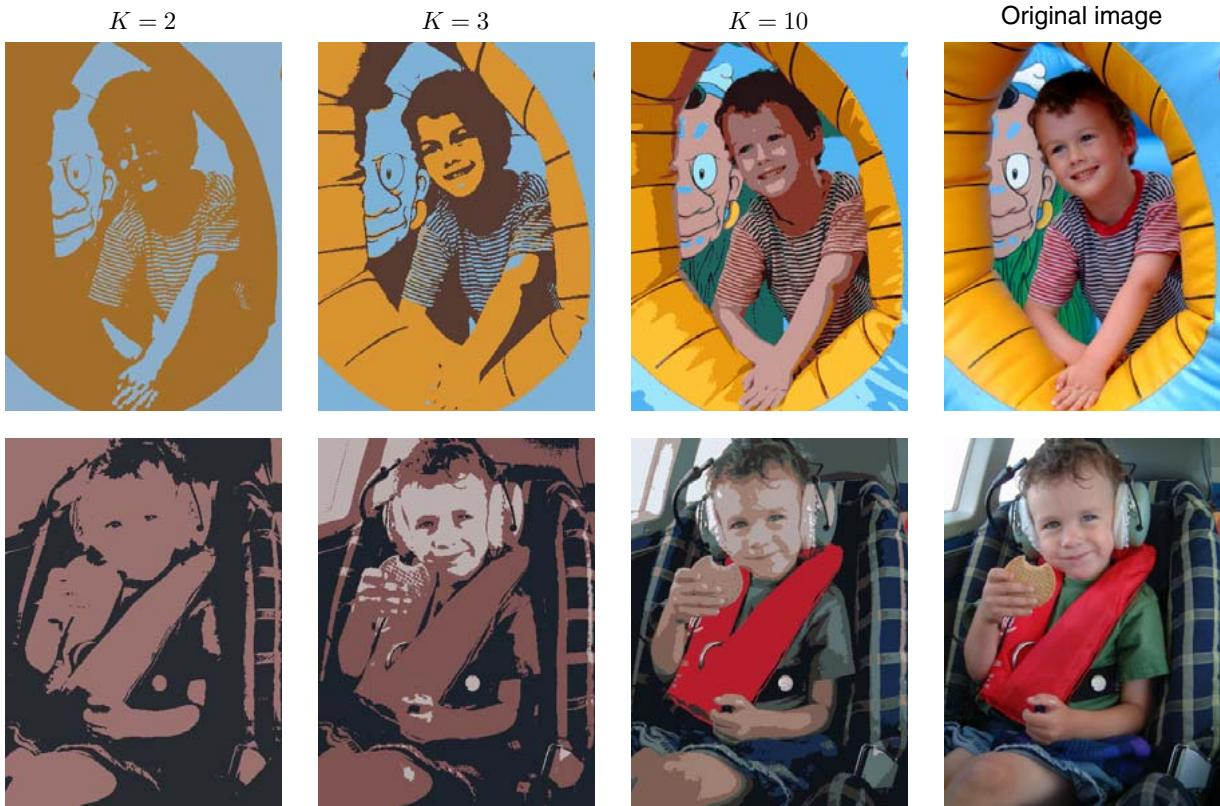
\includegraphics[keepaspectratio,alt={image}]{images/244a77a61012f24ac49d71f242722d2d9fa9953eee6b2d3f3f7f5a0bae3ba46a.jpg}}

Figure 9.3 Two examples of the application of the K-means clustering
algorithm to image segmentation showing the initial images together with
their K-means segmentations obtained using various values of K. This
also illustrates of the use of vector quantization for data compression,
in which smaller values of K give higher compression at the expense of
poorer image quality.

We can also use the result of a clustering algorithm to perform data
compression. It is important to distinguish between lossless data
compression, in which the goal is to be able to reconstruct the original
data exactly from the compressed representation, and lossy data
compression, in which we accept some errors in the reconstruction in
return for higher levels of compression than can be achieved in the
lossless case. We can apply the K-means algorithm to the problem of
lossy data compression as follows. For each of the N data points, we
store only the identity k of the cluster to which it is assigned. We
also store the values of the K cluster centres \(\pmb { \mu } _ { k }\)
, which typically requires significantly less data, provided we choose
\(K \ll N\) . Each data point is then approximated by its nearest centre
\(\pmb { \mu } _ { k }\) . New data points can similarly be compressed
by first finding the nearest \(\pmb { \mu } _ { k }\) and then storing
the label k instead of the original data vector. This framework is often
called vector quantization, and the vectors \(\mu _ { k }\) are called
code-book vectors.

The image segmentation problem discussed above also provides an
illustration of the use of clustering for data compression. Suppose the
original image has N pixels comprising \(\{ R , { \cal G } , B \}\)
values each of which is stored with 8 bits of precision. Then to
transmit the whole image directly would cost 24N bits. Now suppose we
first run K-means on the image data, and then instead of transmitting
the original pixel intensity vectors we transmit the identity of the
nearest vector \(\pmb { \mu } _ { k }\) . Because there are K such
vectors, this requires log K bits per pixel. We must also transmit the K
code book vectors \(\pmb { \mu } _ { k }\) , which requires 24K bits,
and so the total number of bits required to transmit the image is
\(2 \bar { 4 } K + N \log _ { 2 } K\) (rounding up to the nearest
integer). The original image shown in Figure 9.3 has
\(2 4 0 \times 1 8 0 = 4 3\) , 200 pixels and so requires
\(2 4 \times 4 3 , 2 0 0 = 1 , 0 3 6\) , 800 bits to transmit directly.
By comparison, the compressed images require 43, 248 bits \(( K = 2 )\)
, 86, 472 bits \(( K = 3 )\) , and 173, 040 bits \(( K = 1 0 )\) ,
respectively, to transmit. These represent compression ratios compared
to the original image of 4.2\%, 8.3\%, and 16.7\%, respectively. We see
that there is a trade-off between degree of compression and image
quality. Note that our aim in this example is to illustrate the K-means
algorithm. If we had been aiming to produce a good image compressor,
then it would be more fruitful to consider small blocks of adjacent
pixels, for instance \(5 \times 5\) , and thereby exploit the
correlations that exist in natural images between nearby pixels.

\subsection{9.2. Mixtures of Gaussians}\label{mixtures-of-gaussians}

In Section 2.3.9 we motivated the Gaussian mixture model as a simple
linear superposition of Gaussian components, aimed at providing a richer
class of density models than the single Gaussian. We now turn to a
formulation of Gaussian mixtures in terms of discrete latent variables.
This will provide us with a deeper insight into this important
distribution, and will also serve to motivate the
expectation-maximization algorithm.

Recall from (2.188) that the Gaussian mixture distribution can be
written as a linear superposition of Gaussians in the form

\[
p (\mathbf {x}) = \sum_ {k = 1} ^ {K} \pi_ {k} \mathcal {N} (\mathbf {x} | \boldsymbol {\mu} _ {k}, \boldsymbol {\Sigma} _ {k}).\tag{9.7}
\]

Let us introduce a K-dimensional binary random variable z having a
1-of-K representation in which a particular element \(z _ { k }\) is
equal to 1 and all other elements are equal to 0. The values of
\(z _ { k }\) therefore satisfy \(z _ { k } \in \{ 0 , 1 \}\) and
\(\textstyle \sum _ { k } z _ { k } = 1\) , and we see that there are K
possible states for the vector z according to which element is nonzero.
We shall define the joint distribution
\(p ( \mathbf { x } , \mathbf { z } )\) in terms of a marginal
distribution \(p ( \mathbf { z } )\) and a conditional distribution
\(p ( \mathbf { x } | \mathbf { z } )\) , corresponding to the graphical
model in Figure 9.4. The marginal distribution over z is specified in
terms of the mixing coefficients \(\pi _ { k }\) , such that

\[
p (z _ {k} = 1) = \pi_ {k}
\]

Figure 9.4 Graphical representation of a mixture model, in which the
joint distribution is expressed in the form
\(p ( \mathbf { x } , \mathbf { z } ) \ =\)
\(p ( \mathbf { z } ) p ( \mathbf { x } | \mathbf { z } )\)

\pandocbounded{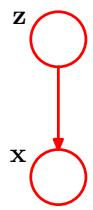
\includegraphics[keepaspectratio,alt={image}]{images/90414c10649ae5d37ac6e58c73051addda74b6732836eb2c208773a7ecd5152e.jpg}}

where the parameters \(\left\{ \pi _ { k } \right\}\) must satisfy

\[
0 \leqslant \pi_ {k} \leqslant 1\tag{9.8}
\]

together with

\[
\sum_ {k = 1} ^ {K} \pi_ {k} = 1\tag{9.9}
\]

in order to be valid probabilities. Because z uses a 1-of-K
representation, we can also write this distribution in the form

\[
p (\mathbf {z}) = \prod_ {k = 1} ^ {K} \pi_ {k} ^ {z _ {k}}.\tag{9.10}
\]

Similarly, the conditional distribution of x given a particular value
for z is a Gaussian

\[
p (\mathbf {x} | z _ {k} = 1) = \mathcal {N} (\mathbf {x} | \pmb {\mu} _ {k}, \pmb {\Sigma} _ {k})
\]

which can also be written in the form

\[
p (\mathbf {x} | \mathbf {z}) = \prod_ {k = 1} ^ {K} \mathcal {N} (\mathbf {x} | \boldsymbol {\mu} _ {k}, \boldsymbol {\Sigma} _ {k}) ^ {z _ {k}}.\tag{9.11}
\]

Exercise 9.3

The joint distribution is given by
\(p ( \mathbf { z } ) p ( \mathbf { x } | \mathbf { z } )\) , and the
marginal distribution of x is then obtained by summing the joint
distribution over all possible states of z to give

\[
p (\mathbf {x}) = \sum_ {\mathbf {z}} p (\mathbf {z}) p (\mathbf {x} | \mathbf {z}) = \sum_ {k = 1} ^ {K} \pi_ {k} \mathcal {N} (\mathbf {x} | \boldsymbol {\mu} _ {k}, \boldsymbol {\Sigma} _ {k})\tag{9.12}
\]

where we have made use of (9.10) and (9.11). Thus the marginal
distribution of x is a Gaussian mixture of the form (9.7). If we have
several observations
\(\mathbf { x } _ { 1 } , \ldots , \mathbf { x } _ { N }\) then, because
we have represented the marginal distribution in the form
\(p ( \mathbf { x } ) \mathbf { \alpha } = \mathbf { \alpha }\)
\(\begin{array} { r } { \sum _ { \mathbf { z } } p ( \mathbf { x } , \mathbf { z } ) } \end{array}\)
, it follows that for every observed data point \({ \bf x } _ { n }\)
there is a corresponding latent variable \(\mathbf { z } _ { n }\)

We have therefore found an equivalent formulation of the Gaussian
mixture involving an explicit latent variable. It might seem that we
have not gained much by doing so. However, we are now able to work with
the joint distribution \(p ( \mathbf { x } , \mathbf { z } )\)

instead of the marginal distribution \(p ( \mathbf { x } )\) , and this
will lead to significant simplifications, most notably through the
introduction of the expectation-maximization (EM) algorithm.

Another quantity that will play an important role is the conditional
probability of z given x. We shall use
\(\gamma ( \boldsymbol { z } _ { k } )\) to denote
\(p ( z _ { k } = 1 | \mathbf { x } )\) , whose value can be found using
Bayes' theorem

\[
\begin{array}{l l l} \gamma (z _ {k}) \equiv p (z _ {k} = 1 | \mathbf {x}) & = & \frac {p (z _ {k} = 1) p (\mathbf {x} | z _ {k} = 1)}{K} \\ & & \sum_ {j = 1} ^ {K} p (z _ {j} = 1) p (\mathbf {x} | z _ {j} = 1) \\ & = & \frac {\pi_ {k} \mathcal {N} (\mathbf {x} | \boldsymbol {\mu} _ {k} , \boldsymbol {\Sigma} _ {k})}{K}. \\ & & \sum_ {j = 1} ^ {K} \pi_ {j} \mathcal {N} (\mathbf {x} | \boldsymbol {\mu} _ {j}, \boldsymbol {\Sigma} _ {j}) \end{array}\tag{9.13}
\]

We shall view \(\pi _ { k }\) as the prior probability of
\(z _ { k } = 1\) , and the quantity
\(\gamma ( \boldsymbol { z } _ { k } )\) as the corresponding posterior
probability once we have observed x. As we shall see later,
\(\gamma ( \boldsymbol { z } _ { k } )\) can also be viewed as the
responsibility that component k takes for `explaining' the observation
x.

We can use the technique of ancestral sampling to generate random
samples distributed according to the Gaussian mixture model. To do this,
we first generate a value for \(\mathbf { z } ,\) which we denote
\({ \widehat { \mathbf { z } } } ,\) , from the marginal distribution
\(p ( \mathbf { z } )\) and then generate a value for x from the
conditional distribution
\(p ( \mathbf { x } | \widehat { \mathbf { z } } )\) . Techniques for
sampling from standard distributions are discussed in Chapter 11. We can
depict samples from the joint distribution
\(p ( \mathbf { x } , \mathbf { z } )\) by plotting points at the
corresponding values of x and then colouring them according to the value
of \(\mathbf { z } ,\) in other words according to which Gaussian
component was responsible for generating them, as shown in Figure
9.5(a). Similarly samples from the marginal distribution
\(p ( \mathbf { x } )\) are obtained by taking the samples from the
joint distribution and ignoring the values of \(\mathbf { z } .\) .
These are illustrated in Figure 9.5(b) by plotting the x values without
any coloured labels.

We can also use this synthetic data set to illustrate the
`responsibilities' by evaluating, for every data point, the posterior
probability for each component in the mixture distribution from which
this data set was generated. In particular, we can represent the value
of the responsibilities \(\gamma ( z _ { n k } )\) associated with data
point \({ \bf x } _ { n }\) by plotting the corresponding point using
proportions of red, blue, and green ink given by
\(\gamma ( z _ { n k } )\) for \(k = 1 , 2 , 3\) , respectively, as
shown in Figure 9.5(c). So, for instance, a data point for which
\(\gamma ( z _ { n 1 } ) = 1\) will be coloured red, whereas one for
which \(\gamma ( z _ { n 2 } ) = \gamma ( z _ { n 3 } ) = 0 . 5\) will
be coloured with equal proportions of blue and green ink and so will
appear cyan. This should be compared with Figure 9.5(a) in which the
data points were labelled using the true identity of the component from
which they were generated.

\subsection{9.2.1 Maximum likelihood}\label{maximum-likelihood}

Suppose we have a data set of observations
\(\left\{ \mathbf { x } _ { 1 } , \ldots , \mathbf { x } _ { N } \right\}\)
, and we wish to model this data using a mixture of Gaussians. We can
represent this data set as an \(N \times D\) matrix X in which the
\(n ^ { \mathrm { t h } }\) row is given by
\({ \bf x } _ { n } ^ { \mathrm { T } }\) . Similarly, the corresponding
latent variables will be denoted by an \(N \times K\) matrix Z with rows
\({ \bf z } _ { n } ^ { \mathrm { T } }\) . If we assume that the data
points are drawn independently from the distribution, then we can
express the Gaussian mixture model for this i.i.d. data set using the
graphical representation shown in Figure 9.6. From (9.7) the log of the
likelihood function is given by

\pandocbounded{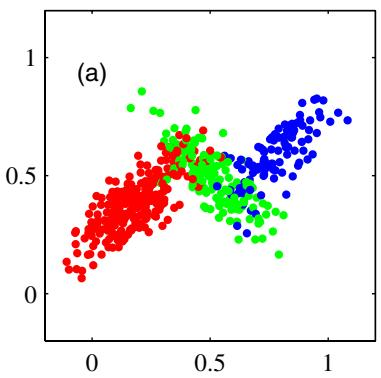
\includegraphics[keepaspectratio,alt={image}]{images/969a89938ba9ac45196dddc96694b7f9babfb815ed6230e7b353d5a05af44221.jpg}}

\pandocbounded{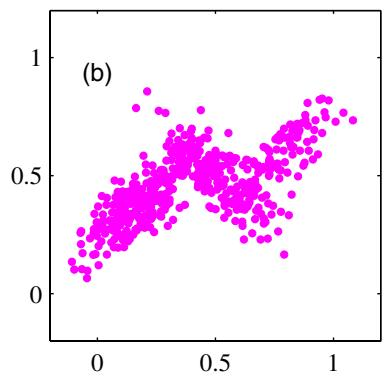
\includegraphics[keepaspectratio,alt={image}]{images/1ef6e9428d040574efa4c33a43b62af9d818d8c0a323e49b463976d5b9bc791f.jpg}}

\pandocbounded{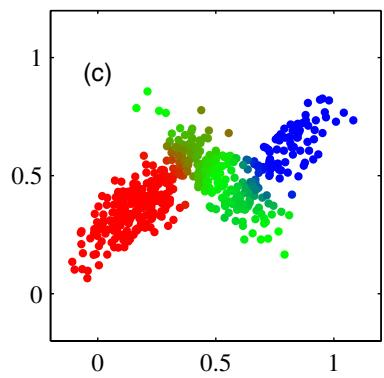
\includegraphics[keepaspectratio,alt={image}]{images/6c624a1745e46a8625168afdade1d3681f3c7519945536df0ce267f031d912c2.jpg}}

Figure 9.5 Example of 500 points drawn from the mixture of 3 Gaussians
shown in Figure 2.23. (a) Samples from the joint distribution
\(p ( \mathbf { z } ) p ( \mathbf { x } | \mathbf { z } )\) in which the
three states of z, corresponding to the three components of the mixture,
are depicted in red, green, and blue, and (b) the corresponding samples
from the marginal distribution \(p ( \mathbf { x } )\) , which is
obtained by simply ignoring the values of z and just plotting the x
values. The data set in (a) is said to be complete, whereas that in (b)
is incomplete. (c) The same samples in which the colours represent the
value of the responsibilities \(\gamma ( z _ { n k } )\) associated with
data point \(\mathbf { x } _ { n } ,\) obtained by plotting the
corresponding point using proportions of red, blue, and green ink given
by \(\gamma ( z _ { n k } )\) for \(k = 1\) , 2, 3, respectively

\[
\ln p (\mathbf {X} | \boldsymbol {\pi}, \boldsymbol {\mu}, \boldsymbol {\Sigma}) = \sum_ {n = 1} ^ {N} \ln \left\{\sum_ {k = 1} ^ {K} \pi_ {k} \mathcal {N} (\mathbf {x} _ {n} | \boldsymbol {\mu} _ {k}, \boldsymbol {\Sigma} _ {k}) \right\}.\tag{9.14}
\]

Before discussing how to maximize this function, it is worth emphasizing
that there is a significant problem associated with the maximum
likelihood framework applied to Gaussian mixture models, due to the
presence of singularities. For simplicity, consider a Gaussian mixture
whose components have covariance matrices given by
\(\boldsymbol { \Sigma } _ { k } = \sigma _ { k } ^ { 2 } \mathbf { I }\)
, where I is the unit matrix, although the conclusions will hold for
general covariance matrices. Suppose that one of the components of the
mixture model, let us say the \(j ^ { \mathrm { t h } }\) component, has
its mean \(\mu _ { j }\) exactly equal to one of the data points so that
\(\pmb { \mu } _ { j } = \mathbf { x } _ { n }\) for some value of
n.~This data point will then contribute a term in the likelihood
function of the form

Figure 9.6 Graphical representation of a Gaussian mixture model for a
set of N i.i.d. data points \(\left\{ \mathbf { x } _ { n } \right\}\) ,
with corresponding latent points
\(\left\{ \mathbf { z } _ { n } \right\}\) , where
\(n = 1 , \ldots , N\)

\pandocbounded{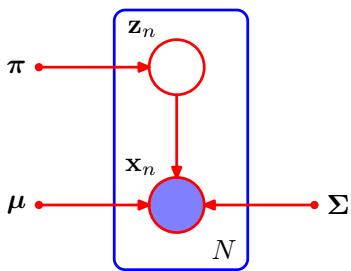
\includegraphics[keepaspectratio,alt={image}]{images/9fa2aee5eacef67df44d4fc08f58aa53eb8647b063cfa4486c06e667d31ceffa.jpg}}

Illustration of how singularities in the likelihood function arise with
mixtures of Gaussians. This should be compared with the case of a single
Gaussian shown in Figure 1.14 for which no singularities arise.

\pandocbounded{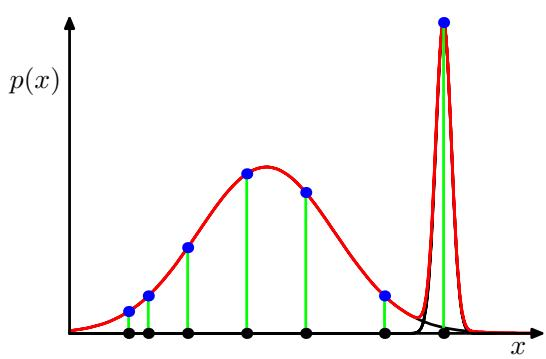
\includegraphics[keepaspectratio,alt={image}]{images/a6aab490203f69cf1375561ab12ddbe67b5dba00609c23f92338526c5e9dc732.jpg}}

\[
\mathcal {N} (\mathbf {x} _ {n} | \mathbf {x} _ {n}, \sigma_ {j} ^ {2} \mathbf {I}) = \frac {1}{(2 \pi) ^ {1 / 2}} \frac {1}{\sigma_ {j}}.\tag{9.15}
\]

If we consider the limit \(\sigma _ { j } \ \to \ 0\) , then we see that
this term goes to infinity and so the log likelihood function will also
go to infinity. Thus the maximization of the log likelihood function is
not a well posed problem because such singularities will always be
present and will occur whenever one of the Gaussian components
`collapses' onto a specific data point. Recall that this problem did not
arise in the case of a single Gaussian distribution. To understand the
difference, note that if a single Gaussian collapses onto a data point
it will contribute multiplicative factors to the likelihood function
arising from the other data points and these factors will go to zero
exponentially fast, giving an overall likelihood that goes to zero
rather than infinity. However, once we have (at least) two components in
the mixture, one of the components can have a finite variance and
therefore assign finite probability to all of the data points while the
other component can shrink onto one specific data point and thereby
contribute an ever increasing additive value to the log likelihood. This
is illustrated in Figure 9.7. These singularities provide another
example of the severe over-fitting that can occur in a maximum
likelihood approach. We shall see that this difficulty does not occur if
we adopt a Bayesian approach. For the moment, however, we simply note
that in applying maximum likelihood to Gaussian mixture models we must
take steps to avoid finding such pathological solutions and instead seek
local maxima of the likelihood function that are well behaved. We can
hope to avoid the singularities by using suitable heuristics, for
instance by detecting when a Gaussian component is collapsing and
resetting its mean to a randomly chosen value while also resetting its
covariance to some large value, and then continuing with the
optimization.

A further issue in finding maximum likelihood solutions arises from the
fact that for any given maximum likelihood solution, a K-component
mixture will have a total of K! equivalent solutions corresponding to
the K! ways of assigning K sets of parameters to K components. In other
words, for any given (nondegenerate) point in the space of parameter
values there will be a further \(K ! - 1\) additional points all of
which give rise to exactly the same distribution. This problem is known
as identifiability (Casella and Berger, 2002) and is an important issue
when we wish to interpret the parameter values discovered by a model.
Identifiability will also arise when we discuss models having continuous
latent variables in Chapter 12. However, for the purposes of finding a
good density model, it is irrelevant because any of the equivalent
solutions is as good as any other.

Maximizing the log likelihood function (9.14) for a Gaussian mixture
model turns out to be a more complex problem than for the case of a
single Gaussian. The difficulty arises from the presence of the
summation over k that appears inside the logarithm in (9.14), so that
the logarithm function no longer acts directly on the Gaussian. If we
set the derivatives of the log likelihood to zero, we will no longer
obtain a closed form solution, as we shall see shortly.

One approach is to apply gradient-based optimization techniques
(Fletcher, 1987; Nocedal and Wright, 1999; Bishop and Nabney, 2008).
Although gradient-based techniques are feasible, and indeed will play an
important role when we discuss mixture density networks in Chapter 5, we
now consider an alternative approach known as the EM algorithm which has
broad applicability and which will lay the foundations for a discussion
of variational inference techniques in Chapter 10.

\subsection{9.2.2 EM for Gaussian
mixtures}\label{em-for-gaussian-mixtures}

An elegant and powerful method for finding maximum likelihood solutions
for models with latent variables is called the expectation-maximization
algorithm, or EM algorithm (Dempster et al., 1977; McLachlan and
Krishnan, 1997). Later we shall give a general treatment of EM, and we
shall also show how EM can be generalized to obtain the variational
inference framework. Initially, we shall motivate the EM algorithm by
giving a relatively informal treatment in the context of the Gaussian
mixture model. We emphasize, however, that EM has broad applicability,
and indeed it will be encountered in the context of a variety of
different models in this book.

Let us begin by writing down the conditions that must be satisfied at a
maximum of the likelihood function. Setting the derivatives of ln
\(p ( { \bf X } | \pi , \mu , \Sigma )\) in (9.14) with respect to the
means \(\mu _ { k }\) of the Gaussian components to zero, we obtain

\[
0 = - \sum_ {n = 1} ^ {N} \underbrace {\frac {\pi_ {k} \mathcal {N} (\mathbf {x} _ {n} | \boldsymbol {\mu} _ {k} , \boldsymbol {\Sigma} _ {k})}{\sum_ {j} \pi_ {j} \mathcal {N} (\mathbf {x} _ {n} | \boldsymbol {\mu} _ {j} , \boldsymbol {\Sigma} _ {j})}} _ {\gamma (z _ {n k})} \boldsymbol {\Sigma} _ {k} (\mathbf {x} _ {n} - \boldsymbol {\mu} _ {k})\tag{9.16}
\]

where we have made use of the form (2.43) for the Gaussian distribution.
Note that the posterior probabilities, or responsibilities, given by
(9.13) appear naturally on the right-hand side. Multiplying by
\(\Sigma _ { k } ^ { - 1 }\) (which we assume to be nonsingular) and
rearranging we obtain

\[
\pmb {\mu} _ {k} = \frac {1}{N _ {k}} \sum_ {n = 1} ^ {N} \gamma (z _ {n k}) \mathbf {x} _ {n}\tag{9.17}
\]

where we have defined

\[
N _ {k} = \sum_ {n = 1} ^ {N} \gamma (z _ {n k}).\tag{9.18}
\]

We can interpret \(N _ { k }\) as the effective number of points
assigned to cluster k. Note carefully the form of this solution. We see
that the mean \(\mu _ { k }\) for the \(k ^ { \mathrm { t h } }\)
Gaussian component is obtained by taking a weighted mean of all of the
points in the data set, in which the weighting factor for data point
\({ \bf x } _ { n }\) is given by the posterior probability
\(\gamma ( z _ { n k } )\) that component k was responsible for
generating \({ \bf x } _ { n }\)

If we set the derivative of ln \(p ( { \bf X } | \pi , \mu , \Sigma )\)
with respect to \(\Sigma _ { k }\) to zero, and follow a similar line of
reasoning, making use of the result for the maximum likelihood solution
for the covariance matrix of a single Gaussian, we obtain

\[
\pmb {\Sigma} _ {k} = \frac {1}{N _ {k}} \sum_ {n = 1} ^ {N} \gamma (z _ {n k}) (\mathbf {x} _ {n} - \pmb {\mu} _ {k}) (\mathbf {x} _ {n} - \pmb {\mu} _ {k}) ^ {\mathrm{T}}\tag{9.19}
\]

which has the same form as the corresponding result for a single
Gaussian fitted to the data set, but again with each data point weighted
by the corresponding posterior probability and with the denominator
given by the effective number of points associated with the
corresponding component.

Finally, we maximize ln \(p ( { \bf X } | \pi , \mu , \Sigma )\) with
respect to the mixing coefficients \(\pi _ { k }\) . Here we must take
account of the constraint (9.9), which requires the mixing coefficients
to sum to one. This can be achieved using a Lagrange multiplier and
maximizing the following quantity

\[
\ln p (\mathbf {X} | \boldsymbol {\pi}, \boldsymbol {\mu}, \boldsymbol {\Sigma}) + \lambda \left(\sum_ {k = 1} ^ {K} \pi_ {k} - 1\right)\tag{9.20}
\]

which gives

\[
0 = \sum_ {n = 1} ^ {N} \frac {\mathcal {N} (\mathbf {x} _ {n} | \boldsymbol {\mu} _ {k} , \boldsymbol {\Sigma} _ {k})}{\sum_ {j} \pi_ {j} \mathcal {N} (\mathbf {x} _ {n} | \boldsymbol {\mu} _ {j} , \boldsymbol {\Sigma} _ {j})} + \lambda\tag{9.21}
\]

where again we see the appearance of the responsibilities. If we now
multiply both sides by \(\pi _ { k }\) and sum over k making use of the
constraint (9.9), we find \(\lambda = - N\) Using this to eliminate λ
and rearranging we obtain

\[
\pi_ {k} = \frac {N _ {k}}{N}\tag{9.22}
\]

so that the mixing coefficient for the \(k ^ { \mathrm { t h } }\)
component is given by the average responsibility which that component
takes for explaining the data points.

It is worth emphasizing that the results (9.17), (9.19), and (9.22) do
not constitute a closed-form solution for the parameters of the mixture
model because the responsibilities \(\gamma ( z _ { n k } )\) depend on
those parameters in a complex way through (9.13). However, these results
do suggest a simple iterative scheme for finding a solution to the
maximum likelihood problem, which as we shall see turns out to be an
instance of the EM algorithm for the particular case of the Gaussian
mixture model. We first choose some initial values for the means,
covariances, and mixing coefficients. Then we alternate between the
following two updates that we shall call the E step and the M step, for
reasons that will become apparent shortly. In the expectation step, or E
step, we use the current values for the parameters to evaluate the
posterior probabilities, or responsibilities, given by (9.13). We then
use these probabilities in the maximization step, or M step, to
re-estimate the means, covariances, and mixing coefficients using the
results (9.17), (9.19), and (9.22). Note that in so doing we first
evaluate the new means using (9.17) and then use these new values to
find the covariances using (9.19), in keeping with the corresponding
result for a single Gaussian distribution. We shall show that each
update to the parameters resulting from an E step followed by an M step
is guaranteed to increase the log likelihood function. In practice, the
algorithm is deemed to have converged when the change in the log
likelihood function, or alternatively in the parameters, falls below
some threshold. We illustrate the EM algorithm for a mixture of two
Gaussians applied to the rescaled Old Faithful data set in Figure 9.8.
Here a mixture of two Gaussians is used, with centres initialized using
the same values as for the K-means algorithm in Figure 9.1, and with
precision matrices initialized to be proportional to the unit matrix.
Plot (a) shows the data points in green, together with the initial
configuration of the mixture model in which the one standard-deviation
contours for the two

\pandocbounded{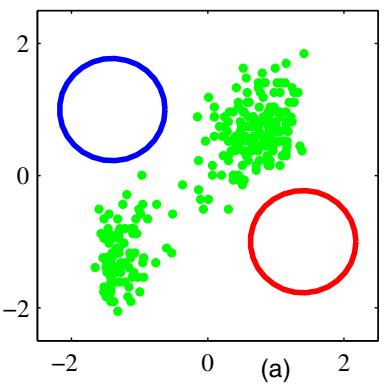
\includegraphics[keepaspectratio,alt={image}]{images/e599f8c3d1a536c459c1540c242dcfe1872418bc4ff3a477e7445824a77512c7.jpg}}

\pandocbounded{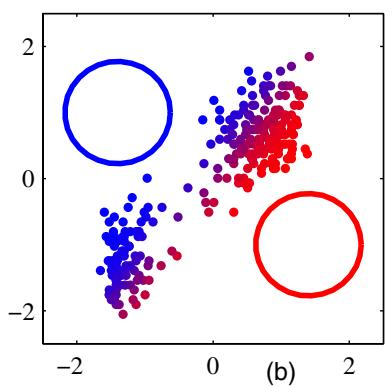
\includegraphics[keepaspectratio,alt={image}]{images/36233150eb8fd2d14bffe6916f1ae283d95e329a24e41da6f48c0cbf7c11c29a.jpg}}

\pandocbounded{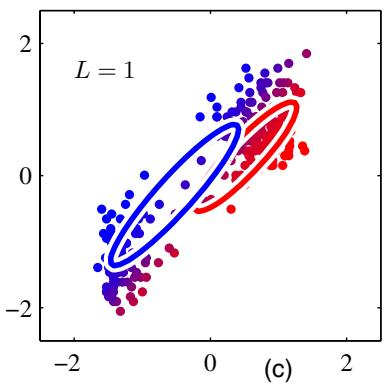
\includegraphics[keepaspectratio,alt={image}]{images/da15c71d77212971f03552117c7a7d695c4e082ee23eecdc7884eeab909cb2eb.jpg}}

\pandocbounded{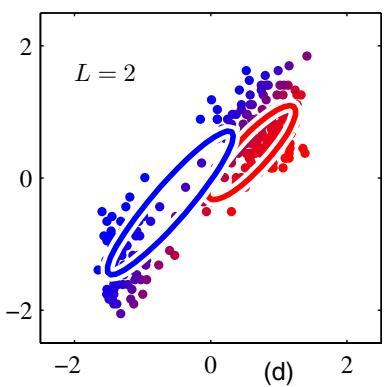
\includegraphics[keepaspectratio,alt={image}]{images/a5524f2cb65b79792f748bec0324f8931d6d3c0c0c0ee94a54ae96a01081e5c9.jpg}}

\pandocbounded{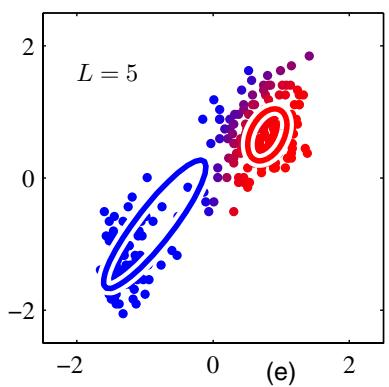
\includegraphics[keepaspectratio,alt={image}]{images/1fed2ad9db669b4a7d4d4a31f203ea83059ef3f475f34f76e8a247fdb1cd3fa5.jpg}}

\pandocbounded{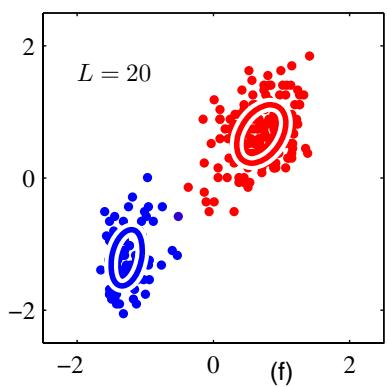
\includegraphics[keepaspectratio,alt={image}]{images/1030baaae01b121b411b7b97962732af71a20ddf999364674b423c5cf04b0fd0.jpg}}

Figure 9.8 Illustration of the EM algorithm using the Old Faithful set
as used for the illustration of the K-means algorithm in Figure 9.1. See
the text for details.

Gaussian components are shown as blue and red circles. Plot (b) shows
the result of the initial E step, in which each data point is depicted
using a proportion of blue ink equal to the posterior probability of
having been generated from the blue component, and a corresponding
proportion of red ink given by the posterior probability of having been
generated by the red component. Thus, points that have a significant
probability for belonging to either cluster appear purple. The situation
after the first M step is shown in plot (c), in which the mean of the
blue Gaussian has moved to the mean of the data set, weighted by the
probabilities of each data point belonging to the blue cluster, in other
words it has moved to the centre of mass of the blue ink. Similarly, the
covariance of the blue Gaussian is set equal to the covariance of the
blue ink. Analogous results hold for the red component. Plots (d), (e),
and (f) show the results after 2, 5, and 20 complete cycles of EM,
respectively. In plot (f) the algorithm is close to convergence.

Note that the EM algorithm takes many more iterations to reach
(approximate) convergence compared with the K-means algorithm, and that
each cycle requires significantly more computation. It is therefore
common to run the K-means algorithm in order to find a suitable
initialization for a Gaussian mixture model that is subsequently adapted
using EM. The covariance matrices can conveniently be initialized to the
sample covariances of the clusters found by the K-means algorithm, and
the mixing coefficients can be set to the fractions of data points
assigned to the respective clusters. As with gradient-based approaches
for maximizing the log likelihood, techniques must be employed to avoid
singularities of the likelihood function in which a Gaussian component
collapses onto a particular data point. It should be emphasized that
there will generally be multiple local maxima of the log likelihood
function, and that EM is not guaranteed to find the largest of these
maxima. Because the EM algorithm for Gaussian mixtures plays such an
important role, we summarize it below.

\subsection{EM for Gaussian Mixtures}\label{em-for-gaussian-mixtures-1}

Given a Gaussian mixture model, the goal is to maximize the likelihood
function with respect to the parameters (comprising the means and
covariances of the components and the mixing coefficients).

\begin{enumerate}
\def\labelenumi{\arabic{enumi}.}
\item
  Initialize the means \(\mu _ { k }\) , covariances \(\Sigma _ { k }\)
  and mixing coefficients \(\pi _ { k }\) , and evaluate the initial
  value of the log likelihood.
\item
  E step. Evaluate the responsibilities using the current parameter
  values
\end{enumerate}

\[
\gamma (z _ {n k}) = \frac {\pi_ {k} \mathcal {N} (\mathbf {x} _ {n} | \boldsymbol {\mu} _ {k} , \boldsymbol {\Sigma} _ {k})}{\sum_ {j = 1} ^ {K} \pi_ {j} \mathcal {N} (\mathbf {x} _ {n} | \boldsymbol {\mu} _ {j} , \boldsymbol {\Sigma} _ {j})}.\tag{9.23}
\]

\begin{enumerate}
\def\labelenumi{\arabic{enumi}.}
\setcounter{enumi}{2}
\tightlist
\item
  M step. Re-estimate the parameters using the current responsibilities
\end{enumerate}

\[
{\pmb {\mu} _ {k} ^ {\mathrm{new}}} = {\frac {1}{N _ {k}} \sum_ {n = 1} ^ {N} \gamma (z _ {n k}) \mathbf {x} _ {n}}\tag{9.24}
\]

\[
{\pmb {\Sigma} _ {k} ^ {\mathrm{new}}} = {\frac {1}{N _ {k}} \sum_ {n = 1} ^ {N} \gamma (z _ {n k}) (\mathbf {x} _ {n} - \pmb {\mu} _ {k} ^ {\mathrm{new}}) (\mathbf {x} _ {n} - \pmb {\mu} _ {k} ^ {\mathrm{new}}) ^ {\mathrm{T}}}\tag{9.25}
\]

\[
\pi_ {k} ^ {\mathrm{new}} = \frac {N _ {k}}{N}\tag{9.26}
\]

where

\[
N _ {k} = \sum_ {n = 1} ^ {N} \gamma (z _ {n k}).\tag{9.27}
\]

\begin{enumerate}
\def\labelenumi{\arabic{enumi}.}
\setcounter{enumi}{3}
\tightlist
\item
  Evaluate the log likelihood
\end{enumerate}

\[
\ln p (\mathbf {X} | \boldsymbol {\mu}, \boldsymbol {\Sigma}, \boldsymbol {\pi}) = \sum_ {n = 1} ^ {N} \ln \left\{\sum_ {k = 1} ^ {K} \pi_ {k} \mathcal {N} (\mathbf {x} _ {n} | \boldsymbol {\mu} _ {k}, \boldsymbol {\Sigma} _ {k}) \right\}\tag{9.28}
\]

and check for convergence of either the parameters or the log
likelihood. If the convergence criterion is not satisfied return to step
2.

\subsection{9.3. An Alternative View of
EM}\label{an-alternative-view-of-em}

In this section, we present a complementary view of the EM algorithm
that recognizes the key role played by latent variables. We discuss this
approach first of all in an abstract setting, and then for illustration
we consider once again the case of Gaussian mixtures.

The goal of the EM algorithm is to find maximum likelihood solutions for
models having latent variables. We denote the set of all observed data
by X, in which the \(n ^ { \mathrm { t h } }\) row represents
\(\mathbf { x } _ { n } ^ { \mathrm { { T } } } .\) , and similarly we
denote the set of all latent variables by Z, with a corresponding row
\({ \mathbf z } _ { n } ^ { \mathrm { T } }\) . The set of all model
parameters is denoted by θ, and so the log likelihood function is given
by

\[
\ln p (\mathbf {X} | \boldsymbol {\theta}) = \ln \left\{\sum_ {\mathbf {Z}} p (\mathbf {X}, \mathbf {Z} | \boldsymbol {\theta}) \right\}.\tag{9.29}
\]

Note that our discussion will apply equally well to continuous latent
variables simply by replacing the sum over Z with an integral.

A key observation is that the summation over the latent variables
appears inside the logarithm. Even if the joint distribution
\(p ( \mathbf { X } , \mathbf { Z } | \boldsymbol { \theta } )\) belongs
to the exponential family, the marginal distribution
\(p ( \mathbf { X } | \pmb { \theta } )\) typically does not as a result
of this summation. The presence of the sum prevents the logarithm from
acting directly on the joint distribution, resulting in complicated
expressions for the maximum likelihood solution.

Now suppose that, for each observation in X, we were told the
corresponding value of the latent variable Z. We shall call
\(\{ \mathbf { X } , \mathbf { Z } \}\) the complete data set, and we
shall refer to the actual observed data X as incomplete, as illustrated
in Figure 9.5. The likelihood function for the complete data set simply
takes the form ln
\(p ( \mathbf { X } , \mathbf { Z } | \boldsymbol { \theta } )\) and we
shall suppose that maximization of this complete-data log likelihood
function is straightforward.

In practice, however, we are not given the complete data set
\(\{ \mathbf { X } , \mathbf { Z } \}\) , but only the incomplete data
X. Our state of knowledge of the values of the latent variables in Z is
given only by the posterior distribution
\(p ( \mathbf { Z } | \mathbf { X } , \pmb \theta )\) . Because we
cannot use the complete-data log likelihood, we consider instead its
expected value under the posterior distribution of the latent variable,
which corresponds (as we shall see) to the E step of the EM algorithm.
In the subsequent M step, we maximize this expectation. If the current
estimate for the parameters is denoted
\(\theta ^ { \mathrm { o l d } }\) , then a pair of successive E and M
steps gives rise to a revised estimate
\(\pmb { \theta } ^ { \mathrm { n e w } }\) . The algorithm is
initialized by choosing some starting value for the parameters
\(\theta _ { 0 }\) . The use of the expectation may seem somewhat
arbitrary. However, we shall see the motivation for this choice when we
give a deeper treatment of EM in Section 9.4.

In the E step, we use the current parameter values
\(\theta ^ { \mathrm { o l d } }\) to find the posterior distribution of
the latent variables given by
\(p ( { \bf Z } | { \bf X } , \boldsymbol { \theta } ^ { \mathrm { o l d } } )\)
. We then use this posterior distribution to find the expectation of the
complete-data log likelihood evaluated for some general parameter value
θ. This expectation, denoted
\(\mathcal { Q } ( \theta , \theta ^ { \mathrm { o l d } } )\) , is
given by

\[
\mathcal {Q} (\boldsymbol {\theta}, \boldsymbol {\theta} ^ {\mathrm{old}}) = \sum_ {\mathbf {Z}} p (\mathbf {Z} | \mathbf {X}, \boldsymbol {\theta} ^ {\mathrm{old}}) \ln p (\mathbf {X}, \mathbf {Z} | \boldsymbol {\theta}).\tag{9.30}
\]

In the M step, we determine the revised parameter estimate
\(\pmb { \theta } ^ { \mathrm { n e w } }\) by maximizing this function

\[
\boldsymbol {\theta} ^ {\text { new }} = \underset {\boldsymbol {\theta}} {\arg \max} \mathcal {Q} (\boldsymbol {\theta}, \boldsymbol {\theta} ^ {\text { old }}).\tag{9.31}
\]

Note that in the definition of
\(\mathcal { Q } ( \theta , \theta ^ { \mathrm { o l d } } )\) , the
logarithm acts directly on the joint distribution
\(p ( \mathbf { X } , \mathbf { Z } | \boldsymbol { \theta } )\) , and
so the corresponding M-step maximization will, by supposition, be
tractable.

The general EM algorithm is summarized below. It has the property, as we
shall show later, that each cycle of EM will increase the
incomplete-data log likelihood (unless it is already at a local
maximum).

\subsection{The General EM Algorithm}\label{the-general-em-algorithm}

Given a joint distribution
\(p ( \mathbf { X } , \mathbf { Z } | \boldsymbol { \theta } )\) over
observed variables X and latent variables Z, governed by parameters θ,
the goal is to maximize the likelihood function
\(p ( \mathbf { X } | \pmb { \theta } )\) with respect to
\(\pmb { \theta } .\)

\begin{enumerate}
\def\labelenumi{\arabic{enumi}.}
\item
  Choose an initial setting for the parameters
  \(\pmb { \theta } ^ { \mathrm { o l d } }\)
\item
  E step Evaluate
  \(p ( { \bf Z } | { \bf X } , \boldsymbol { \theta } ^ { \mathrm { o l d } } )\)
\item
  M step Evaluate \(\pmb { \theta } ^ { \mathrm { n e w } }\) given by
\end{enumerate}

\[
\boldsymbol {\theta} ^ {\text { new }} = \underset {\boldsymbol {\theta}} {\arg \max} \mathcal {Q} (\boldsymbol {\theta}, \boldsymbol {\theta} ^ {\text { old }})\tag{9.32}
\]

where

\[
\mathcal {Q} (\pmb {\theta}, \pmb {\theta} ^ {\mathrm{old}}) = \sum_ {\mathbf {Z}} p (\mathbf {Z} | \mathbf {X}, \pmb {\theta} ^ {\mathrm{old}}) \ln p (\mathbf {X}, \mathbf {Z} | \pmb {\theta}).\tag{9.33}
\]

\begin{enumerate}
\def\labelenumi{\arabic{enumi}.}
\setcounter{enumi}{3}
\tightlist
\item
  Check for convergence of either the log likelihood or the parameter
  values. If the convergence criterion is not satisfied, then let
\end{enumerate}

\[
\boldsymbol {\theta} ^ {\mathrm{old}} \leftarrow \boldsymbol {\theta} ^ {\mathrm{new}}\tag{9.34}
\]

and return to step 2.

The EM algorithm can also be used to find MAP (maximum posterior)
solutions for models in which a prior \(p ( \pmb \theta )\) is defined
over the parameters. In this case the E step remains the same as in the
maximum likelihood case, whereas in the M step the quantity to be
maximized is given by
\(\mathcal { Q } ( \pmb { \theta } , \pmb { \theta } ^ { \mathrm { o l d } } ) + \ln p ( \pmb { \theta } )\)
. Suitable choices for the prior will remove the singularities of the
kind illustrated in Figure 9.7.

Here we have considered the use of the EM algorithm to maximize a
likelihood function when there are discrete latent variables. However,
it can also be applied when the unobserved variables correspond to
missing values in the data set. The distribution of the observed values
is obtained by taking the joint distribution of all the variables and
then marginalizing over the missing ones. EM can then be used to
maximize the corresponding likelihood function. We shall show an example
of the application of this technique in the context of principal
component analysis in Figure 12.11. This will be a valid procedure if
the data values are missing at random, meaning that the mechanism
causing values to be missing does not depend on the unobserved values.
In many situations this will not be the case, for instance if a sensor
fails to return a value whenever the quantity it is measuring exceeds
some threshold.

\subsection{9.3.1 Gaussian mixtures
revisited}\label{gaussian-mixtures-revisited}

We now consider the application of this latent variable view of EM to
the specific case of a Gaussian mixture model. Recall that our goal is
to maximize the log likelihood function (9.14), which is computed using
the observed data set X, and we saw that this was more difficult than
for the case of a single Gaussian distribution due to the presence of
the summation over k that occurs inside the logarithm. Suppose then that
in addition to the observed data set X, we were also given the values of
the corresponding discrete variables Z. Recall that Figure 9.5(a) shows
a `complete' data set (i.e., one that includes labels showing which
component generated each data point) while Figure 9.5(b) shows the
corresponding `incomplete' data set. The graphical model for the
complete data is shown in Figure 9.9.

Figure 9.9 This shows the same graph as in Figure 9.6 except that we now
suppose that the discrete variables \(\mathbf { z } _ { n }\) are
observed, as well as the data variables \({ \bf x } _ { n }\)

\pandocbounded{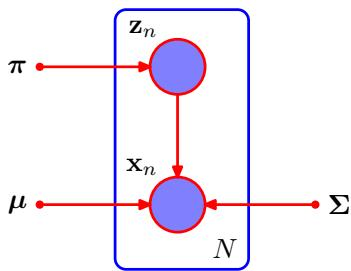
\includegraphics[keepaspectratio,alt={image}]{images/48c86602b9eae618bb2b59dd5591b8fc2c09091b1adb6cee495d389f1d021c1b.jpg}}

Now consider the problem of maximizing the likelihood for the complete
data set X, Z . From (9.10) and (9.11), this likelihood function takes
the form

\[
p (\mathbf {X}, \mathbf {Z} | \boldsymbol {\mu}, \boldsymbol {\Sigma}, \boldsymbol {\pi}) = \prod_ {n = 1} ^ {N} \prod_ {k = 1} ^ {K} \pi_ {k} ^ {z _ {n k}} \mathcal {N} (\mathbf {x} _ {n} | \boldsymbol {\mu} _ {k}, \boldsymbol {\Sigma} _ {k}) ^ {z _ {n k}}\tag{9.35}
\]

where \(z _ { n k }\) denotes the \(k ^ { \mathrm { t h } }\) component
of \(\mathbf { z } _ { n }\) . Taking the logarithm, we obtain

\[
\ln p (\mathbf {X}, \mathbf {Z} | \boldsymbol {\mu}, \boldsymbol {\Sigma}, \boldsymbol {\pi}) = \sum_ {n = 1} ^ {N} \sum_ {k = 1} ^ {K} z _ {n k} \left\{\ln \pi_ {k} + \ln \mathcal {N} (\mathbf {x} _ {n} | \boldsymbol {\mu} _ {k}, \boldsymbol {\Sigma} _ {k}) \right\}.\tag{9.36}
\]

Comparison with the log likelihood function (9.14) for the incomplete
data shows that the summation over k and the logarithm have been
interchanged. The logarithm now acts directly on the Gaussian
distribution, which itself is a member of the exponential family. Not
surprisingly, this leads to a much simpler solution to the maximum
likelihood problem, as we now show. Consider first the maximization with
respect to the means and covariances. Because \(\mathbf { z } _ { n }\)
is a \(K \cdot\) -dimensional vector with all elements equal to 0 except
for a single element having the value 1, the complete-data log
likelihood function is simply a sum of K independent contributions, one
for each mixture component. Thus the maximization with respect to a mean
or a covariance is exactly as for a single Gaussian, except that it
involves only the subset of data points that are `assigned' to that
component. For the maximization with respect to the mixing coefficients,
we note that these are coupled for different values of k by virtue of
the summation constraint (9.9). Again, this can be enforced using a
Lagrange multiplier as before, and leads to the result

\[
\pi_ {k} = \frac {1}{N} \sum_ {n = 1} ^ {N} z _ {n k}\tag{9.37}
\]

so that the mixing coefficients are equal to the fractions of data
points assigned to the corresponding components.

Thus we see that the complete-data log likelihood function can be
maximized trivially in closed form. In practice, however, we do not have
values for the latent variables so, as discussed earlier, we consider
the expectation, with respect to the posterior distribution of the
latent variables, of the complete-data log likelihood.

Using (9.10) and (9.11) together with Bayes' theorem, we see that this
posterior distribution takes the form

\[
p (\mathbf {Z} | \mathbf {X}, \boldsymbol {\mu}, \boldsymbol {\Sigma}, \boldsymbol {\pi}) \propto \prod_ {n = 1} ^ {N} \prod_ {k = 1} ^ {K} [ \pi_ {k} \mathcal {N} (\mathbf {x} _ {n} | \boldsymbol {\mu} _ {k}, \boldsymbol {\Sigma} _ {k}) ] ^ {z _ {n k}}.\tag{9.38}
\]

and hence factorizes over n so that under the posterior distribution the
\(\left\{ { { \bf { z } } _ { n } } \right\}\) are independent. This is
easily verified by inspection of the directed graph in Figure 9.6 and
making use of the d-separation criterion. The expected value of the
indicator variable \(z _ { n k }\) under this posterior distribution is
then given by

\[
\begin{array}{r c l} \mathbb {E} [ z _ {n k} ] & = & \frac {\sum_ {z _ {n k}} z _ {n k} \left[ \pi_ {k} \mathcal {N} (\mathbf {x} _ {n} | \boldsymbol {\mu} _ {k} , \boldsymbol {\Sigma} _ {k}) \right] ^ {z _ {n k}}}{\sum_ {z _ {n j}} \left[ \pi_ {j} \mathcal {N} (\mathbf {x} _ {n} | \boldsymbol {\mu} _ {j} , \boldsymbol {\Sigma} _ {j}) \right] ^ {z _ {n j}}} \\ & = & \frac {\pi_ {k} \mathcal {N} (\mathbf {x} _ {n} | \boldsymbol {\mu} _ {k} , \boldsymbol {\Sigma} _ {k})}{\sum_ {j = 1} ^ {K} \pi_ {j} \mathcal {N} (\mathbf {x} _ {n} | \boldsymbol {\mu} _ {j} , \boldsymbol {\Sigma} _ {j})} = \gamma (z _ {n k}) \end{array}\tag{9.39}
\]

which is just the responsibility of component k for data point
\({ \bf x } _ { n }\) . The expected value of the complete-data log
likelihood function is therefore given by

\[
\mathbb {E} _ {\mathbf {Z}} [ \ln p (\mathbf {X}, \mathbf {Z} | \boldsymbol {\mu}, \boldsymbol {\Sigma}, \boldsymbol {\pi}) ] = \sum_ {n = 1} ^ {N} \sum_ {k = 1} ^ {K} \gamma (z _ {n k}) \left\{\ln \pi_ {k} + \ln \mathcal {N} (\mathbf {x} _ {n} | \boldsymbol {\mu} _ {k}, \boldsymbol {\Sigma} _ {k}) \right\}.\tag{9.40}
\]

We can now proceed as follows. First we choose some initial values for
the parameters
\(\mu ^ { \mathrm { o l d } } , \Sigma ^ { \mathrm { o l d } }\) and
\(\pi ^ { \mathrm { o l d } }\) , and use these to evaluate the
responsibilities (the E step). We then keep the responsibilities fixed
and maximize (9.40) with respect to \(\mu _ { k } , \Sigma _ { k }\) and
\(\pi _ { k }\) (the M step). This leads to closed form solutions for
\(\mu ^ { \mathrm { n e w } } , \bar { \Sigma } ^ { \mathrm { n e w } }\)
and \(\pi ^ { \mathrm { n e w } }\) given by (9.17), (9.19), and (9.22)
as before. This is precisely the EM algorithm for Gaussian mixtures as
derived earlier. We shall gain more insight into the role of the
expected complete-data log likelihood function when we give a proof of
convergence of the EM algorithm in Section 9.4.

\subsection{9.3.2 Relation to K-means}\label{relation-to-k-means}

Comparison of the K-means algorithm with the EM algorithm for Gaussian
mixtures shows that there is a close similarity. Whereas the K-means
algorithm performs a hard assignment of data points to clusters, in
which each data point is associated uniquely with one cluster, the EM
algorithm makes a soft assignment based on the posterior probabilities.
In fact, we can derive the K-means algorithm as a particular limit of EM
for Gaussian mixtures as follows.

Consider a Gaussian mixture model in which the covariance matrices of
the mixture components are given by I, where  is a variance parameter
that is shared by all of the components, and I is the identity matrix,
so that

\[
p (\mathbf {x} | \boldsymbol {\mu} _ {k}, \boldsymbol {\Sigma} _ {k}) = \frac {1}{(2 \pi \epsilon) ^ {1 / 2}} \exp \left\{- \frac {1}{2 \epsilon} \| \mathbf {x} - \boldsymbol {\mu} _ {k} \| ^ {2} \right\}.\tag{9.41}
\]

We now consider the EM algorithm for a mixture of K Gaussians of this
form in which we treat  as a fixed constant, instead of a parameter to
be re-estimated. From (9.13) the posterior probabilities, or
responsibilities, for a particular data point \({ \bf x } _ { n }\) are
given by

\[
\gamma (z _ {n k}) = \frac {\pi_ {k} \exp \left\{- \| \mathbf {x} _ {n} - \pmb {\mu} _ {k} \| ^ {2} / 2 \epsilon \right\}}{\sum_ {j} \pi_ {j} \exp \left\{- \| \mathbf {x} _ {n} - \pmb {\mu} _ {j} \| ^ {2} / 2 \epsilon \right\}}.\tag{9.42}
\]

If we consider the limit \(\epsilon  0\) , we see that in the
denominator the term for which
\(\| \mathbf { x } _ { n } - { \pmb { \mu } } _ { i } \| ^ { 2 }\) is
smallest will go to zero most slowly, and hence the responsibilities
\(\gamma ( z _ { n k } )\) for the data point \({ \bf x } _ { n }\) all
go to zero except for term \(j ,\) , for which the responsibility
\(\gamma ( z _ { n j } )\) will go to unity. Note that this holds
independently of the values of the \(\pi _ { k }\) so long as none of
the \(\pi _ { k }\) is zero. Thus, in this limit, we obtain a hard
assignment of data points to clusters, just as in the K-means algorithm,
so that \(\gamma ( z _ { n k } ) \to r _ { n k }\) where \(r _ { n k }\)
is defined by (9.2). Each data point is thereby assigned to the cluster
having the closest mean.

The EM re-estimation equation for the \(\mu _ { k }\) , given by (9.17),
then reduces to the K-means result (9.4). Note that the re-estimation
formula for the mixing coefficients (9.22) simply re-sets the value of
\(\pi _ { k }\) to be equal to the fraction of data points assigned to
cluster \(k ,\) although these parameters no longer play an active role
in the algorithm.

Finally, in the limit \(\epsilon  0\) the expected complete-data log
likelihood, given by (9.40), becomes

\[
\mathbb {E} _ {\mathbf {Z}} [ \ln p (\mathbf {X}, \mathbf {Z} | \boldsymbol {\mu}, \boldsymbol {\Sigma}, \boldsymbol {\pi}) ] \rightarrow - \frac {1}{2} \sum_ {n = 1} ^ {N} \sum_ {k = 1} ^ {K} r _ {n k} \| \mathbf {x} _ {n} - \boldsymbol {\mu} _ {k} \| ^ {2} + \mathrm{const.}\tag{9.43}
\]

Thus we see that in this limit, maximizing the expected complete-data
log likelihood is equivalent to minimizing the distortion measure J for
the K-means algorithm given by (9.1).

Note that the K-means algorithm does not estimate the covariances of the
clusters but only the cluster means. A hard-assignment version of the
Gaussian mixture model with general covariance matrices, known as the
elliptical K-means algorithm, has been considered by Sung and Poggio
(1994).

\subsection{9.3.3 Mixtures of Bernoulli
distributions}\label{mixtures-of-bernoulli-distributions}

So far in this chapter, we have focussed on distributions over
continuous variables described by mixtures of Gaussians. As a further
example of mixture modelling, and to illustrate the EM algorithm in a
different context, we now discuss mixtures of discrete binary variables
described by Bernoulli distributions. This model is also known as latent
class analysis (Lazarsfeld and Henry, 1968; McLachlan and Peel, 2000).
As well as being of practical importance in its own right, our
discussion of Bernoulli mixtures will also lay the foundation for a
consideration of hidden Markov models over discrete variables.

Consider a set of D binary variables \(x _ { i }\) , where
\(i = 1 , \ldots , D\) , each of which is governed by a Bernoulli
distribution with parameter \(\mu _ { i }\) , so that

\[
p (\mathbf {x} | \boldsymbol {\mu}) = \prod_ {i = 1} ^ {D} \mu_ {i} ^ {x _ {i}} (1 - \mu_ {i}) ^ {(1 - x _ {i})}\tag{9.44}
\]

where
\({ \bf x } = ( x _ { 1 } , \dots , x _ { D } ) ^ { \mathrm { T } }\)
and
\(\pmb { \mu } = ( \mu _ { 1 } , \ldots , \mu _ { D } ) ^ { \mathrm { T } }\)
. We see that the individual variables \(x _ { i }\) are independent,
given \(\pmb { \mu } .\) . The mean and covariance of this distribution
are easily seen to be

\[
\mathbb {E} [ \mathbf {x} ] = \boldsymbol {\mu}\tag{9.45}
\]

\[
\operatorname{cov} [ \mathbf {x} ] = \operatorname{diag} \{\mu_ {i} (1 - \mu_ {i}) \}.\tag{9.46}
\]

Now let us consider a finite mixture of these distributions given by

\[
p (\mathbf {x} | \boldsymbol {\mu}, \boldsymbol {\pi}) = \sum_ {k = 1} ^ {K} \pi_ {k} p (\mathbf {x} | \boldsymbol {\mu} _ {k})\tag{9.47}
\]

where
\(\pmb { \mu } = \{ \pmb { \mu } _ { 1 } , \ldots , \pmb { \mu } _ { K } \} , \pmb { \pi } = \{ \pi _ { 1 } , \ldots , \pi _ { K } \}\)
, and

\[
p (\mathbf {x} | \boldsymbol {\mu} _ {k}) = \prod_ {i = 1} ^ {D} \mu_ {k i} ^ {x _ {i}} (1 - \mu_ {k i}) ^ {(1 - x _ {i})}.\tag{9.48}
\]

Exercise 9.12

The mean and covariance of this mixture distribution are given by

\[
\begin{array}{r c l} \mathbb {E} [ \mathbf {x} ] & = & \sum_ {k = 1} ^ {K} \pi_ {k} \boldsymbol {\mu} _ {k} \\ \operatorname{cov} [ \mathbf {x} ] & = & \sum_ {k = 1} ^ {K} \pi_ {k} \left\{\boldsymbol {\Sigma} _ {k} + \boldsymbol {\mu} _ {k} \boldsymbol {\mu} _ {k} ^ {\mathrm{T}} \right\} - \mathbb {E} [ \mathbf {x} ] \mathbb {E} [ \mathbf {x} ] ^ {\mathrm{T}} \end{array}\tag{9.49}
\]

(9.50)

where Σ = diag \(\{ \mu _ { k i } ( 1 - \mu _ { k i } ) \}\) . Because
the covariance matrix \(\mathrm { c o v } [ \mathbf { x } ]\) is no
longer diagonal, the mixture distribution can capture correlations
between the variables, unlike a single Bernoulli distribution.

If we are given a data set
\(\mathbf { X } = \{ \mathbf { x } _ { 1 } , \ldots , \mathbf { x } _ { N } \}\)
then the log likelihood function for this model is given by

\[
\ln p (\mathbf {X} | \boldsymbol {\mu}, \boldsymbol {\pi}) = \sum_ {n = 1} ^ {N} \ln \left\{\sum_ {k = 1} ^ {K} \pi_ {k} p \left(\mathbf {x} _ {n} \mid \boldsymbol {\mu} _ {k}\right) \right\}.\tag{9.51}
\]

Again we see the appearance of the summation inside the logarithm, so
that the maximum likelihood solution no longer has closed form.

We now derive the EM algorithm for maximizing the likelihood function
for the mixture of Bernoulli distributions. To do this, we first
introduce an explicit latent

Exercise 9.14

variable z associated with each instance of x. As in the case of the
Gaussian mixture,
\(\mathbf { z } = ( z _ { 1 } , \dots , z _ { K } ) ^ { \mathrm { T } }\)
is a binary K-dimensional variable having a single component equal to 1,
with all other components equal to 0. We can then write the conditional
distribution of x, given the latent variable, as

\[
p (\mathbf {x} | \mathbf {z}, \boldsymbol {\mu}) = \prod_ {k = 1} ^ {K} p (\mathbf {x} | \boldsymbol {\mu} _ {k}) ^ {z _ {k}}\tag{9.52}
\]

while the prior distribution for the latent variables is the same as for
the mixture of Gaussians model, so that

\[
p (\mathbf {z} | \boldsymbol {\pi}) = \prod_ {k = 1} ^ {K} \pi_ {k} ^ {z _ {k}}.\tag{9.53}
\]

If we form the product of \(p ( \mathbf { x } | \mathbf { z } , \mu )\)
and \(p ( \mathbf { z } | \boldsymbol { \pi } )\) and then marginalize
over z, then we recover (9.47).

In order to derive the EM algorithm, we first write down the
complete-data log likelihood function, which is given by

\[
\begin{array}{l} \ln p (\mathbf {X}, \mathbf {Z} | \boldsymbol {\mu}, \boldsymbol {\pi}) = \sum_ {n = 1} ^ {N} \sum_ {k = 1} ^ {K} z _ {n k} \left\{\ln \pi_ {k} \right. \\ \left. + \sum_ {i = 1} ^ {D} [ x _ {n i} \ln \mu_ {k i} + (1 - x _ {n i}) \ln (1 - \mu_ {k i}) ] \right\} \end{array}\tag{9.54}
\]

where \({ \bf X } = \{ { \bf x } _ { n } \}\) and
\({ \bf Z } = \{ { \bf z } _ { n } \}\) . Next we take the expectation
of the complete-data log likelihood with respect to the posterior
distribution of the latent variables to give

\[
\begin{array}{l} \mathbb {E} _ {\mathbf {Z}} [ \ln p (\mathbf {X}, \mathbf {Z} | \boldsymbol {\mu}, \boldsymbol {\pi}) ] = \sum_ {n = 1} ^ {N} \sum_ {k = 1} ^ {K} \gamma (z _ {n k}) \left\{\ln \pi_ {k} \right. \\ \left. + \sum_ {i = 1} ^ {D} \left[ x _ {n i} \ln \mu_ {k i} + (1 - x _ {n i}) \ln (1 - \mu_ {k i}) \right] \right\} \end{array}\tag{9.55}
\]

where \(\gamma ( z _ { n k } ) = \mathbb { E } [ z _ { n k } ]\) is the
posterior probability, or responsibility, of component k given data
point \({ \bf x } _ { n }\) . In the E step, these responsibilities are
evaluated using Bayes theorem, which takes the form

\[
\begin{array}{l l l} \gamma (z _ {n k}) = \mathbb {E} [ z _ {n k} ] & = & \frac {\sum_ {z _ {n k}} z _ {n k} \left[ \pi_ {k} p (\mathbf {x} _ {n} | \boldsymbol {\mu} _ {k}) \right] ^ {z _ {n k}}}{\sum_ {z _ {n j}} \left[ \pi_ {j} p (\mathbf {x} _ {n} | \boldsymbol {\mu} _ {j}) \right] ^ {z _ {n j}}} \\ & = & \frac {\pi_ {k} p (\mathbf {x} _ {n} | \boldsymbol {\mu} _ {k})}{\sum_ {j = 1} ^ {K} \pi_ {j} p (\mathbf {x} _ {n} | \boldsymbol {\mu} _ {j})}. \end{array}\tag{9.56}
\]

If we consider the sum over n in (9.55), we see that the
responsibilities enter only through two terms, which can be written as

\[
N _ {k} = \sum_ {n = 1} ^ {N} \gamma (z _ {n k})\tag{9.57}
\]

\[
{\overline {{\mathbf {x}}} _ {k}} = {\frac {1}{N _ {k}} \sum_ {n = 1} ^ {N} \gamma (z _ {n k}) \mathbf {x} _ {n}}\tag{9.58}
\]

where \(N _ { k }\) is the effective number of data points associated
with component k. In the M step, we maximize the expected complete-data
log likelihood with respect to the parameters \(\pmb { \mu } _ { k }\)
and \(\pi .\) . If we set the derivative of (9.55) with respect to
\(\pmb { \mu } _ { k }\) equal to zero and rearrange the terms, we
obtain

\[
\pmb {\mu} _ {k} = \overline {{\mathbf {x}}} _ {k}.\tag{9.59}
\]

We see that this sets the mean of component k equal to a weighted mean
of the data, with weighting coefficients given by the responsibilities
that component k takes for data points. For the maximization with
respect to \(\pi _ { k } .\) , we need to introduce a Lagrange
multiplier to enforce the constraint
\(\dot { \sum _ { k } } \pi _ { k } = 1\) . Following analogous steps to
those used for the mixture of Gaussians, we then obtain

\[
\pi_ {k} = \frac {N _ {k}}{N}\tag{9.60}
\]

which represents the intuitively reasonable result that the mixing
coefficient for component k is given by the effective fraction of points
in the data set explained by that component.

Note that in contrast to the mixture of Gaussians, there are no
singularities in which the likelihood function goes to infinity. This
can be seen by noting that the likelihood function is bounded above
because
\(0 \leqslant p ( \mathbf x _ { n } | \pmb \mu _ { k } ) \leqslant 1\)
There exist singularities at which the likelihood function goes to zero,
but these will not be found by EM provided it is not initialized to a
pathological starting point, because the EM algorithm always increases
the value of the likelihood function, until a local maximum is found. We
illustrate the Bernoulli mixture model in Figure 9.10 by using it to
model handwritten digits. Here the digit images have been turned into
binary vectors by setting all elements whose values exceed 0.5 to 1 and
setting the remaining elements to 0. We now fit a data set of N = 600
such digits, comprising the digits `2', `3', and \(\cdot _ { 4 } ,\) ,
with a mixture of K = 3 Bernoulli distributions by running 10 iterations
of the EM algorithm. The mixing coefficients were initialized to
\(\pi _ { k } = 1 / K\) , and the parameters \(\mu _ { k j }\) were set
to random values chosen uniformly in the range (0.25, 0.75) and then
normalized to satisfy the constraint that
\(\textstyle \sum _ { j } \mu _ { k j } = 1\) We see that a mixture of 3
Bernoulli distributions is able to find the three clusters in the data
set corresponding to the different digits.

The conjugate prior for the parameters of a Bernoulli distribution is
given by the beta distribution, and we have seen that a beta prior is
equivalent to introducing

\pandocbounded{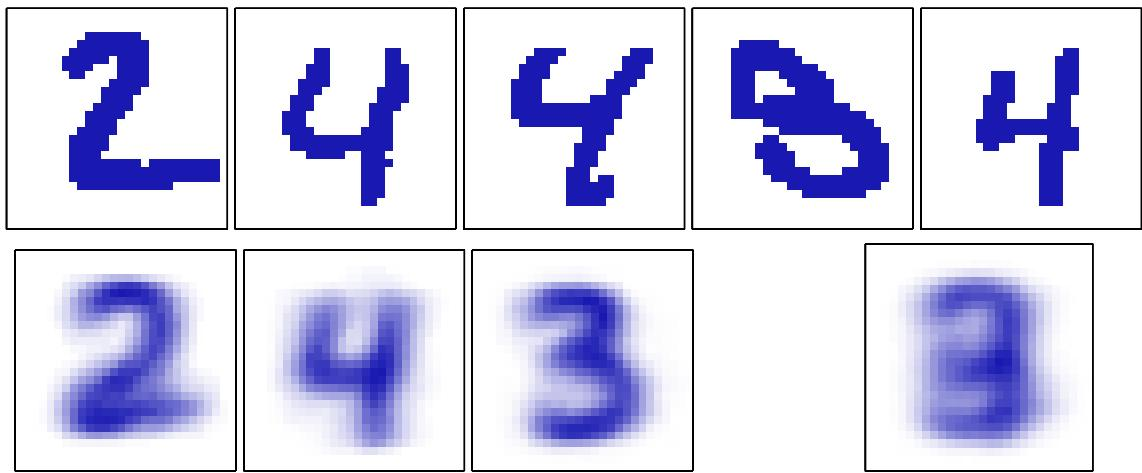
\includegraphics[keepaspectratio,alt={image}]{images/82ada15c9a5b99e91ba12deef072106ffadfcc36aa2dcc540e5e3987f0e903fa.jpg}}

Figure 9.10 Illustration of the Bernoulli mixture model in which the top
row shows examples from the digits data set after converting the pixel
values from grey scale to binary using a threshold of 0.5. On the bottom
row the first three images show the parameters \(\mu _ { k i }\) for
each of the three components in the mixture model. As a comparison, we
also fit the same data set using a single multivariate Bernoulli
distribution, again using maximum likelihood. This amounts to simply
averaging the counts in each pixel and is shown by the right-most image
on the bottom row.

Section 2.1.1

Exercise 9.18

additional effective observations of \(\mathbf { x } .\) We can
similarly introduce priors into the Bernoulli mixture model, and use EM
to maximize the posterior probability distributions.

Exercise 9.19

It is straightforward to extend the analysis of Bernoulli mixtures to
the case of multinomial binary variables having \(M > 2\) states by
making use of the discrete distribution (2.26). Again, we can introduce
Dirichlet priors over the model parameters if desired.

\subsection{9.3.4 EM for Bayesian linear
regression}\label{em-for-bayesian-linear-regression}

As a third example of the application of EM, we return to the evidence
approximation for Bayesian linear regression. In Section 3.5.2, we
obtained the reestimation equations for the hyperparameters α and
\(\beta\) by evaluation of the evidence and then setting the derivatives
of the resulting expression to zero. We now turn to an alternative
approach for finding α and \(\beta\) based on the EM algorithm. Recall
that our goal is to maximize the evidence function
\(p ( \mathbf { t } | \alpha , \beta )\) given by (3.77) with respect to
α and \(\beta .\) Because the parameter vector w is marginalized out, we
can regard it as a latent variable, and hence we can optimize this
marginal likelihood function using EM. In the E step, we compute the
posterior distribution of w given the current setting of the parameters
α and \(\beta\) and then use this to find the expected complete-data log
likelihood. In the M step, we maximize this quantity with respect to α
and β. We have already derived the posterior distribution of w because
this is given by (3.49). The complete-data log likelihood function is
then given by

\[
\ln p (\mathbf {t}, \mathbf {w} | \alpha , \beta) = \ln p (\mathbf {t} | \mathbf {w}, \beta) + \ln p (\mathbf {w} | \alpha)\tag{9.61}
\]

where the likelihood \(p ( \mathbf { t } | \mathbf { w } , \beta )\) and
the prior \(p ( \mathbf { w } | \alpha )\) are given by (3.10) and
(3.52), respectively, and \(y ( \mathbf { x } , \mathbf { w } )\) is
given by (3.3). Taking the expectation with respect to the posterior
distribution of w then gives

\[
\begin{array}{r c l} \mathbb {E} \left[ \ln p (\mathbf {t}, \mathbf {w} | \alpha , \beta) \right] & = & \frac {M}{2} \ln \left(\frac {\alpha}{2 \pi}\right) - \frac {\alpha}{2} \mathbb {E} \left[ \mathbf {w} ^ {\mathrm{T}} \mathbf {w} \right] + \frac {N}{2} \ln \left(\frac {\beta}{2 \pi}\right) \\ & & - \frac {\beta}{2} \sum_ {n = 1} ^ {N} \mathbb {E} \left[ (t _ {n} - \mathbf {w} ^ {\mathrm{T}} \boldsymbol {\phi} _ {n}) ^ {2} \right]. \end{array}\tag{9.62}
\]

Setting the derivatives with respect to α to zero, we obtain the M step
re-estimation equation

\[
\alpha = \frac {M}{\mathbb {E} \left[ \mathbf {w} ^ {\mathrm{T}} \mathbf {w} \right]} = \frac {M}{\mathbf {m} _ {N} ^ {\mathrm{T}} \mathbf {m} _ {N} + \operatorname{Tr} (\mathbf {S} _ {N})}.\tag{9.63}
\]

An analogous result holds for \(\beta .\)

Note that this re-estimation equation takes a slightly different form
from the corresponding result (3.92) derived by direct evaluation of the
evidence function. However, they each involve computation and inversion
(or eigen decomposition) of an \(M \times M\) matrix and hence will have
comparable computational cost per iteration.

These two approaches to determining \(\alpha\) should of course converge
to the same result (assuming they find the same local maximum of the
evidence function). This can be verified by first noting that the
quantity \(\gamma\) is defined by

\[
\gamma = M - \alpha \sum_ {i = 1} ^ {M} \frac {1}{\lambda_ {i} + \alpha} = M - \alpha \operatorname{Tr} (\mathbf {S} _ {N}).\tag{9.64}
\]

At a stationary point of the evidence function, the re-estimation
equation (3.92) will be self-consistently satisfied, and hence we can
substitute for \(\gamma\) to give

\[
\alpha \mathbf {m} _ {N} ^ {\mathrm{T}} \mathbf {m} _ {N} = \gamma = M - \alpha \mathrm{Tr} (\mathbf {S} _ {N})\tag{9.65}
\]

and solving for α we obtain (9.63), which is precisely the EM
re-estimation equation.

As a final example, we consider a closely related model, namely the
relevance vector machine for regression discussed in Section 7.2.1.
There we used direct maximization of the marginal likelihood to derive
re-estimation equations for the hyperparameters α and \(\beta\) . Here
we consider an alternative approach in which we view the weight vector w
as a latent variable and apply the EM algorithm. The E step involves
finding the posterior distribution over the weights, and this is given
by (7.81). In the M step we maximize the expected complete-data log
likelihood, which is defined by

\[
\mathbb {E} _ {\mathbf {w}} \left[ \ln p (\mathbf {t} | \mathbf {X}, \mathbf {w}, \beta) p (\mathbf {w} | \boldsymbol {\alpha}) \right]\tag{9.66}
\]

where the expectation is taken with respect to the posterior
distribution computed using the `old' parameter values. To compute the
new parameter values we maximize with respect to α and \(\beta\) to give

\[
\alpha_ {i} ^ {\mathrm{new}} = \frac {1}{m _ {i} ^ {2} + \Sigma_ {i i}}\tag{9.67}
\]

\[
(\beta^ {\mathrm{new}}) ^ {- 1} = \frac {\| \mathbf {t} - \boldsymbol {\Phi} \mathbf {m} _ {N} \| ^ {2} + \beta^ {- 1} \sum_ {i} \gamma_ {i}}{N}\tag{9.68}
\]

Exercise 9.23

These re-estimation equations are formally equivalent to those obtained
by direct maxmization.

\subsection{9.4. The EM Algorithm in
General}\label{the-em-algorithm-in-general}

The expectation maximization algorithm, or EM algorithm, is a general
technique for finding maximum likelihood solutions for probabilistic
models having latent variables (Dempster et al., 1977; McLachlan and
Krishnan, 1997). Here we give a very general treatment of the EM
algorithm and in the process provide a proof that the EM algorithm
derived heuristically in Sections 9.2 and 9.3 for Gaussian mixtures does
indeed maximize the likelihood function (Csiszar and
Tusn\texttt{ady,\ 1984;\ Hath-} away, 1986; Neal and Hinton, 1999). Our
discussion will also form the basis for the derivation of the
variational inference framework.

Consider a probabilistic model in which we collectively denote all of
the observed variables by X and all of the hidden variables by Z. The
joint distribution
\(p ( \mathbf { X } , \mathbf { Z } | \boldsymbol { \theta } )\) is
governed by a set of parameters denoted \(\pmb { \theta } .\) Our goal
is to maximize the likelihood function that is given by

\[
p (\mathbf {X} | \boldsymbol {\theta}) = \sum_ {\mathbf {Z}} p (\mathbf {X}, \mathbf {Z} | \boldsymbol {\theta}).\tag{9.69}
\]

Here we are assuming Z is discrete, although the discussion is identical
if Z comprises continuous variables or a combination of discrete and
continuous variables, with summation replaced by integration as
appropriate.

We shall suppose that direct optimization of
\(p ( \mathbf { X } | \pmb { \theta } )\) is difficult, but that opti
mization of the complete-data likelihood function
\(p ( \mathbf { X } , \mathbf { Z } | \boldsymbol { \theta } )\) is
significantly easier. Next we introduce a distribution
\(q ( \mathbf { Z } )\) defined over the latent variables, and we
observe that, for any choice of \(q ( \mathbf { Z } )\) , the following
decomposition holds

\[
\ln p (\mathbf {X} | \boldsymbol {\theta}) = \mathcal {L} (q, \boldsymbol {\theta}) + \mathrm{KL} (q \| p)\tag{9.70}
\]

where we have defined

\[
\mathcal {L} (q, \pmb {\theta}) = \sum_ {\mathbf {Z}} q (\mathbf {Z}) \ln \left\{\frac {p (\mathbf {X} , \mathbf {Z} | \pmb {\theta})}{q (\mathbf {Z})} \right\}\tag{9.71}
\]

\[
\operatorname{KL} (q \| p) = - \sum_ {\mathbf {Z}} q (\mathbf {Z}) \ln \left\{\frac {p (\mathbf {Z} | \mathbf {X} , \boldsymbol {\theta})}{q (\mathbf {Z})} \right\}.\tag{9.72}
\]

Note that \(\mathcal { L } ( q , \theta )\) is a functional (see
Appendix D for a discussion of functionals) of the distribution
\(q ( \mathbf { Z } )\) , and a function of the parameters
\(\pmb { \theta } .\) It is worth studying

Illustration of the decomposition given by (9.70), which holds for any
choice of distribution \(q ( \mathbf { Z } )\) Because the
Kullback-Leibler divergence satisfies
\(\mathrm { K L } ( q \| p ) \geqslant 0\) , we see that the quantity
\(\dot { \mathcal { L } } ( \boldsymbol { q } , \boldsymbol { \theta } )\)
is a lower bound on the log likelihood function ln
\(p ( \mathbf { X } | \pmb { \theta } )\)

\pandocbounded{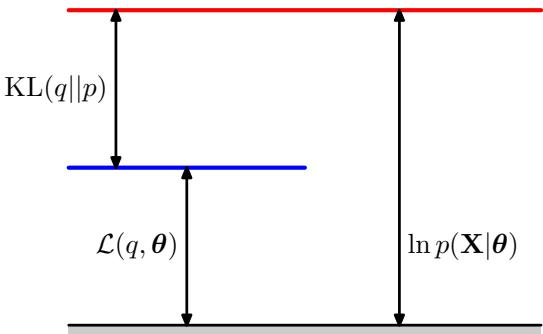
\includegraphics[keepaspectratio,alt={image}]{images/4b9ba213faa93ea2674647d32850b7342d29a29e4006184f72a517147d0ced7c.jpg}}

carefully the forms of the expressions (9.71) and (9.72), and in
particular noting that they differ in sign and also that
\(\mathcal { L } ( q , \theta )\) contains the joint distribution of X
and Z while KL \(\left( q \| p \right)\) contains the conditional
distribution of \(\mathbf { Z }\) given \(\mathbf { X }\) . To verify
the decomposition (9.70), we first make use of the product rule of
probability to give

\[
\ln p (\mathbf {X}, \mathbf {Z} | \boldsymbol {\theta}) = \ln p (\mathbf {Z} | \mathbf {X}, \boldsymbol {\theta}) + \ln p (\mathbf {X} | \boldsymbol {\theta})\tag{9.73}
\]

which we then substitute into the expression for
\(\mathcal { L } ( q , \theta )\) . This gives rise to two terms, one of
which cancels \(\mathrm { K L } ( q \| p )\) while the other gives the
required log likelihood ln \(p ( \mathbf { X } | \pmb { \theta } )\)
after noting that \(q ( \mathbf { Z } )\) is a normalized distribution
that sums to 1.

From (9.72), we see that \(\mathrm { K L } ( q \| p )\) is the
Kullback-Leibler divergence between \(q ( \mathbf { Z } )\) and the
posterior distribution
\(p ( \mathbf { Z } | \mathbf { X } , \pmb \theta )\) . Recall that the
Kullback-Leibler divergence satisfies KL \(( q \| p ) \geqslant 0\) ,
with equality if, and only if,
\(q ( \mathbf { Z } ) = p ( \mathbf { Z } | \mathbf { X } , \theta )\) .
It therefore follows from \(_ { ( 9 . 7 0 ) }\) that
\(\mathcal { L } ( q , \pmb { \theta } ) \leqslant \ln p ( \mathbf { X } | \pmb { \theta } )\)
, in other words that \(\mathcal { L } ( q , \theta )\) is a lower bound
on ln \(p ( \mathbf { X } | \pmb { \theta } )\) . The decomposition
(9.70) is illustrated in Figure 9.11.

The EM algorithm is a two-stage iterative optimization technique for
finding maximum likelihood solutions. We can use the decomposition
(9.70) to define the EM algorithm and to demonstrate that it does indeed
maximize the log likelihood. Suppose that the current value of the
parameter vector is \(\pmb { \theta } ^ { \mathrm { o l d } }\) . In the
E step, the lower bound
\(\mathscr { L } ( q , \theta ^ { \mathrm { o l d } } )\) is maximized
with respect to \(q ( \mathbf { Z } )\) while holding
\(\pmb { \theta } ^ { \mathrm { o l d } }\) fixed. The solution to this
maximization problem is easily seen by noting that the value of ln
\(p ( \mathbf { X } | \mathbf { \theta } ^ { \mathrm { o l d } } )\)
does not depend on \(q ( \mathbf { Z } )\) and so the largest value of
\(\mathcal { L } ( q , \theta ^ { \mathrm { o l d } } )\) will occur
when the Kullback-Leibler divergence vanishes, in other words when
\(q ( \mathbf { Z } )\) is equal to the posterior distribution
\(p ( \mathbf { Z } | \mathbf { X } , \theta ^ { \mathrm { o l d } } )\)
. In this case, the lower bound will equal the log likelihood, as
illustrated in Figure 9.12.

In the subsequent M step, the distribution \(q ( \mathbf { Z } )\) is
held fixed and the lower bound \(\mathcal { L } ( q , \theta )\) is
maximized with respect to \(\pmb \theta\) to give some new value
\(\pmb { \theta } ^ { \mathrm { n e w } }\) This will cause the lower
bound \(\mathcal { L }\) to increase (unless it is already at a
maximum), which will necessarily cause the corresponding log likelihood
function to increase. Because the distribution \(q\) is determined using
the old parameter values rather than the new values and is held fixed
during the M step, it will not equal the new posterior distribution
\(p ( \mathbf { Z } | \mathbf { X } , \pmb { \theta } ^ { \mathrm { n e w } } )\)
, and hence there will be a nonzero KL divergence. The increase in the
log likelihood function is therefore greater than the increase in the
lower bound, as

Illustration of the E step of the EM algorithm. The q distribution is
set equal to the posterior distribution for the current parameter values
\(\pmb { \theta } ^ { \mathrm { o l d } }\) , causing the lower bound to
move up to the same value as the log likelihood function, with the KL
divergence vanishing.

\pandocbounded{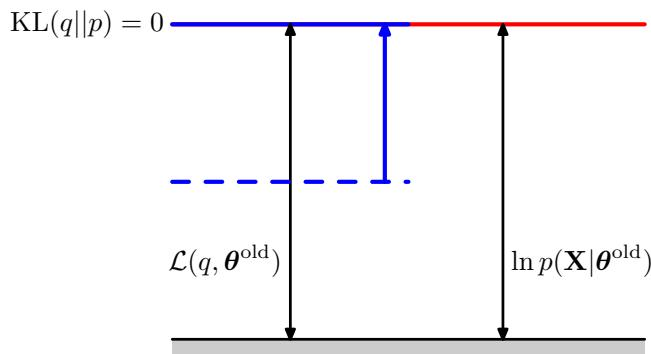
\includegraphics[keepaspectratio,alt={image}]{images/0ff5ad85db3d5f6230dd5d8895da132ef5f12042bf6983fbe70d63ef43ec58fd.jpg}}

shown in Figure 9.13. If we substitute
\(q ( \mathbf { Z } ) = p ( \mathbf { Z } | \mathbf { X } , \theta ^ { \mathrm { o l d } } )\)
into (9.71), we see that, after the E step, the lower bound takes the
form

\[
\begin{array}{r c l} \mathcal {L} (q, \boldsymbol {\theta}) & = & \sum_ {\mathbf {Z}} p (\mathbf {Z} | \mathbf {X}, \boldsymbol {\theta} ^ {\text {old}}) \ln p (\mathbf {X}, \mathbf {Z} | \boldsymbol {\theta}) - \sum_ {\mathbf {Z}} p (\mathbf {Z} | \mathbf {X}, \boldsymbol {\theta} ^ {\text {old}}) \ln p (\mathbf {Z} | \mathbf {X}, \boldsymbol {\theta} ^ {\text {old}}) \\ & = & \mathcal {Q} (\boldsymbol {\theta}, \boldsymbol {\theta} ^ {\text {old}}) + \text {const} \end{array} \tag {9.74}
\]

where the constant is simply the negative entropy of the q distribution
and is therefore independent of θ. Thus in the M step, the quantity that
is being maximized is the expectation of the complete-data log
likelihood, as we saw earlier in the case of mixtures of Gaussians. Note
that the variable \(\pmb \theta\) over which we are optimizing appears
only inside the logarithm. If the joint distribution
\(p ( \mathbf { Z } , \mathbf { X } | \mathbf { \theta } )\) comprises a
member of the exponential family, or a product of such members, then we
see that the logarithm will cancel the exponential and lead to an M step
that will be typically much simpler than the maximization of the
corresponding incomplete-data log likelihood function
\(p ( \mathbf { X } | \pmb { \theta } )\)

The operation of the EM algorithm can also be viewed in the space of
parameters, as illustrated schematically in Figure 9.14. Here the red
curve depicts the (in

Illustration of the M step of the EM algorithm. The distribution
\(q ( \mathbf { Z } )\) is held fixed and the lower bound
\(\mathcal { L } ( q , \theta )\) is maximized with respect to the
parameter vector θ to give a revised value
\(\pmb { \theta } ^ { \mathrm { n e w } }\) . Because the KL divergence
is nonnegative, this causes the log likelihood ln
\(p ( \mathbf { X } | \pmb { \theta } )\) to increase by at least as
much as the lower bound does.

\pandocbounded{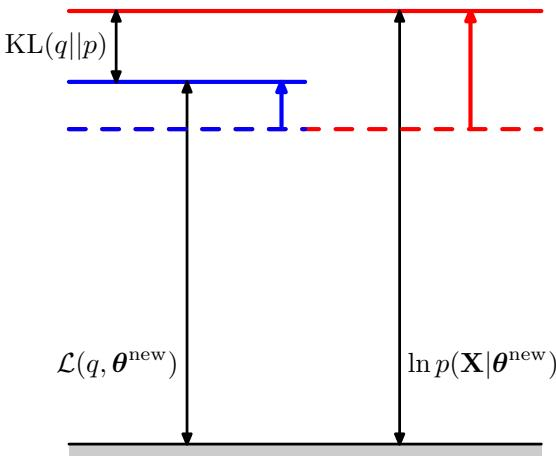
\includegraphics[keepaspectratio,alt={image}]{images/f986fe00455b874bc288930332b443f5a431392205b8f2d9727f43a532696b39.jpg}}

The EM algorithm involves alternately computing a lower bound on the log
likelihood for the current parameter values and then maximizing this
bound to obtain the new parameter values. See the text for a full
discussion.

\pandocbounded{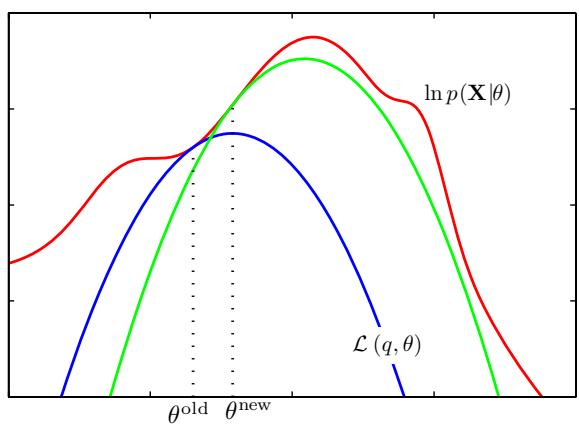
\includegraphics[keepaspectratio,alt={image}]{images/6f1ff9cecd034c1862d063a23de82a295ebe344baf1414992e4465aaabc91fb1.jpg}}

Exercise 9.25

complete data) log likelihood function whose value we wish to maximize.
We start with some initial parameter value
\(\pmb { \theta } ^ { \mathrm { o l d } }\) , and in the first E step we
evaluate the posterior distribution over latent variables, which gives
rise to a lower bound
\({ \mathcal { L } } ( \theta , { \bar { \theta } } ^ { \mathrm { ( o l d ) } } )\)
) whose value equals the log likelihood at
\(\pmb { \theta } ^ { \mathrm { ( o l d ) } }\) , as shown by the blue
curve. Note that the bound makes a tangential contact with the log
likelihood at \(\pmb { \theta } ^ { \mathrm { ( o l d ) } }\) , so that
both curves have the same gradient. This bound is a convex function
having a unique maximum (for mixture components from the exponential
family). In the M step, the bound is maximized giving the value
\(\theta ^ { \mathrm { ( n e w ) } }\) , which gives a larger value of
log likelihood than \(\pmb { \theta } ^ { \mathrm { ( o l d ) } }\) .
The subsequent E step then constructs a bound that is tangential at
\(\theta ^ { \mathrm { ( n e w ) } }\) as shown by the green curve.

For the particular case of an independent, identically distributed data
set, X will comprise N data points
\(\left\{ { \bf x } _ { n } \right\}\) while Z will comprise N
corresponding latent variables \(\left\{ { \bf z } _ { n } \right\}\) ,
where \(n = 1 , \ldots , N\) . From the independence assumption, we have
\(\begin{array} { r } { p ( \mathbf { X } , \mathbf { Z } ) \ = \ \prod _ { n } p ( \mathbf { x } _ { n } , \mathbf { z } _ { n } ) } \end{array}\)
and, by marginalizing over the
\(\left\{ { { \bf { z } } _ { n } } \right\}\) we have
\(p ( \mathbf { X } ) =\) \(\prod _ { n } p ( \mathbf { x } _ { n } )\)
. Using the sum and product rules, we see that the posterior probability
that is evaluated in the E step takes the form

\[
p (\mathbf {Z} | \mathbf {X}, \boldsymbol {\theta}) = \frac {p (\mathbf {X} , \mathbf {Z} | \boldsymbol {\theta})}{\sum_ {\mathbf {Z}} p (\mathbf {X} , \mathbf {Z} | \boldsymbol {\theta})} = \frac {\prod_ {n = 1} ^ {N} p (\mathbf {x} _ {n} , \mathbf {z} _ {n} | \boldsymbol {\theta})}{\sum_ {\mathbf {Z}} \prod_ {n = 1} ^ {N} p (\mathbf {x} _ {n} , \mathbf {z} _ {n} | \boldsymbol {\theta})} = \prod_ {n = 1} ^ {N} p (\mathbf {z} _ {n} | \mathbf {x} _ {n}, \boldsymbol {\theta})\tag{9.75}
\]

and so the posterior distribution also factorizes with respect to n.~In
the case of the Gaussian mixture model this simply says that the
responsibility that each of the mixture components takes for a
particular data point \({ \bf x } _ { n }\) depends only on the value of
\({ \bf x } _ { n }\) and on the parameters θ of the mixture components,
not on the values of the other data points.

We have seen that both the E and the M steps of the EM algorithm are
increasing the value of a well-defined bound on the log likelihood
function and that the complete EM cycle will change the model parameters
in such a way as to cause the log likelihood to increase (unless it is
already at a maximum, in which case the parameters remain unchanged).

We can also use the EM algorithm to maximize the posterior distribution
\(p ( \pmb \theta | \mathbf X )\) for models in which we have introduced
a prior \(p ( \pmb \theta )\) over the parameters. To see this, we note
that as a function of \(\theta _ { ; }\) , we have
\(\bar { p ( { \pmb \theta } | { \bf X } ) } = \bar { p ( { \pmb \theta } , { \bf X } ) / p ( { \bf X } ) }\)
and so

\[
\ln p (\boldsymbol {\theta} | \mathbf {X}) = \ln p (\boldsymbol {\theta}, \mathbf {X}) - \ln p (\mathbf {X}).\tag{9.76}
\]

Making use of the decomposition (9.70), we have

\[
\begin{array}{r c l} \ln p (\boldsymbol {\theta} | \mathbf {X}) & = & \mathcal {L} (q, \boldsymbol {\theta}) + \mathrm{KL} (q \| p) + \ln p (\boldsymbol {\theta}) - \ln p (\mathbf {X}) \\ & \geqslant & \mathcal {L} (q, \boldsymbol {\theta}) + \ln p (\boldsymbol {\theta}) - \ln p (\mathbf {X}). \end{array}\tag{9.77}
\]

where ln \(p ( \mathbf { X } )\) is a constant. We can again optimize
the right-hand side alternately with respect to \(q\) and
\(\pmb { \theta } .\) The optimization with respect to \(q\) gives rise
to the same \(\mathrm { E } \mathrm { - }\) step equations as for the
standard EM algorithm, because \(q\) only appears in
\(\mathcal { L } ( q , \theta )\) The M-step equations are modified
through the introduction of the prior term ln \(p ( \pmb \theta )\)
which typically requires only a small modification to the standard
maximum likelihood M-step equations.

The EM algorithm breaks down the potentially difficult problem of
maximizing the likelihood function into two stages, the E step and the M
step, each of which will often prove simpler to implement. Nevertheless,
for complex models it may be the case that either the E step or the M
step, or indeed both, remain intractable. This leads to two possible
extensions of the EM algorithm, as follows.

The generalized EM, or GEM, algorithm addresses the problem of an
intractable M step. Instead of aiming to maximize
\(\mathcal { L } ( q , \theta )\) with respect to \(\theta ,\) it seeks
instead to change the parameters in such a way as to increase its value.
Again, because \(\mathcal { L } ( q , \theta )\) is a lower bound on the
log likelihood function, each complete EM cycle of the GEM algorithm is
guaranteed to increase the value of the log likelihood (unless the
parameters already correspond to a local maximum). One way to exploit
the GEM approach would be to use one of the nonlinear optimization
strategies, such as the conjugate gradients algorithm, during the M
step. Another form of GEM algorithm, known as the expectation
conditional maximization, or ECM, algorithm, involves making several
constrained optimizations within each M step (Meng and Rubin, 1993). For
instance, the parameters might be partitioned into groups, and the M
step is broken down into multiple steps each of which involves
optimizing one of the subset with the remainder held fixed.

We can similarly generalize the E step of the EM algorithm by performing
a partial, rather than complete, optimization of
\(\mathcal { L } ( q , \theta )\) with respect to
\(q ( \mathbf { Z } )\) (Neal and Hinton, 1999). As we have seen, for
any given value of \(\pmb \theta\) there is a unique maximum of
\(\mathcal { L } ( q , \theta )\) with respect to
\(q ( \mathbf { Z } )\) that corresponds to the posterior distribution
\(q _ { \pmb { \theta } } ( \mathbf { Z } ) =\)
\(p ( \mathbf { Z } | \mathbf { X } , \pmb \theta )\) and that for this
choice of \(q ( \mathbf { Z } )\) the bound
\(\mathcal { L } ( q , \theta )\) is equal to the log likelihood
function ln \(p ( \mathbf { X } | \pmb { \theta } )\) . It follows that
any algorithm that converges to the global maximum of
\(\mathcal { L } ( q , \theta )\) will find a value of \(\pmb \theta\)
that is also a global maximum of the log likelihood ln
\(p ( \mathbf { X } | \pmb { \theta } )\) . Provided
\(p ( \mathbf { X } , \mathbf { Z } | \boldsymbol { \theta } )\) is a
continuous function of θ then, by continuity, any local maximum of
\(\mathcal { L } ( q , \theta )\) will also be a local maximum of ln
\(p ( \mathbf { X } | \pmb { \theta } )\)

Consider the case of N independent data points
\(\mathbf { x } _ { 1 } , \ldots , \mathbf { x } _ { N }\) with
corresponding latent variables
\(\mathbf { z } _ { 1 } , \ldots , \mathbf { z } _ { N }\) . The joint
distribution
\(p ( \mathbf { X } , \mathbf { Z } | \boldsymbol { \theta } )\)
factorizes over the data points, and this structure can be exploited in
an incremental form of EM in which at each EM cycle only one data point
is processed at a time. In the E step, instead of recomputing the
responsibilities for all of the data points, we just re-evaluate the
responsibilities for one data point. It might appear that the subsequent
M step would require computation involving the responsibilities for all
of the data points. However, if the mixture components are members of
the exponential family, then the responsibilities enter only through
simple sufficient statistics, and these can be updated efficiently.
Consider, for instance, the case of a Gaussian mixture, and suppose we
perform an update for data point m in which the corresponding old and
new values of the responsibilities are denoted
\(\gamma ^ { \mathrm { o l d } } ( z _ { m k } )\) and
\(\gamma ^ { \mathrm { n e w } } ( z _ { m k } )\) . In the M step, the
required sufficient statistics can be updated incrementally. For
instance, for the means the sufficient statistics are defined by (9.17)
and (9.18) from which we obtain

Exercise 9.26

\[
\pmb {\mu} _ {k} ^ {\mathrm{new}} = \pmb {\mu} _ {k} ^ {\mathrm{old}} + \left(\frac {\gamma^ {\mathrm{new}} (z _ {m k}) - \gamma^ {\mathrm{old}} (z _ {m k})}{N _ {k} ^ {\mathrm{new}}}\right) (\mathbf {x} _ {m} - \pmb {\mu} _ {k} ^ {\mathrm{old}})\tag{9.78}
\]

together with

\[
N _ {k} ^ {\mathrm{new}} = N _ {k} ^ {\mathrm{old}} + \gamma^ {\mathrm{new}} (z _ {m k}) - \gamma^ {\mathrm{old}} (z _ {m k}).\tag{9.79}
\]

The corresponding results for the covariances and the mixing
coefficients are analogous.

Thus both the E step and the M step take fixed time that is independent
of the total number of data points. Because the parameters are revised
after each data point, rather than waiting until after the whole data
set is processed, this incremental version can converge faster than the
batch version. Each E or M step in this incremental algorithm is
increasing the value of \(\mathcal { L } ( q , \theta )\) and, as we
have shown above, if the algorithm converges to a local (or global)
maximum of \(\mathcal { L } ( q , \theta )\) , this will correspond to a
local (or global) maximum of the log likelihood function ln
\(p ( \mathbf { X } | \pmb { \theta } )\)

\subsection{Exercises}\label{exercises-1}

9.1 () www Consider the K-means algorithm discussed in Section 9.1. Show
that as a consequence of there being a finite number of possible
assignments for the set of discrete indicator variables \(r _ { n k }\)
, and that for each such assignment there is a unique optimum for the
\(\{ \mu _ { k } \}\) , the K-means algorithm must converge after a
finite number of iterations.

9.2 () Apply the Robbins-Monro sequential estimation procedure described
in Section 2.3.5 to the problem of finding the roots of the regression
function given by the derivatives of J in (9.1) with respect to
\(\mu _ { k }\) . Show that this leads to a stochastic K-means algorithm
in which, for each data point \({ \bf x } _ { n }\) , the nearest
prototype \(\pmb { \mu } _ { k }\) is updated using (9.5).

9.3 () www Consider a Gaussian mixture model in which the marginal
distribution \(p ( \mathbf { z } )\) for the latent variable is given by
(9.10), and the conditional distribution
\(p ( \mathbf { x } | \mathbf { z } )\) for the observed variable is
given by (9.11). Show that the marginal distribution
\(p ( \mathbf { x } )\) , obtained by summing
\(p ( \mathbf { z } ) p ( \mathbf { x } | \mathbf { z } )\) over all
possible values of z, is a Gaussian mixture of the form (9.7).

9.4 () Suppose we wish to use the EM algorithm to maximize the posterior
distribution over parameters \(p ( \pmb \theta | \mathbf X )\) for a
model containing latent variables, where X is the observed data set.
Show that the E step remains the same as in the maximum likelihood case,
whereas in the M step the quantity to be maximized is given by
\(\mathcal { Q } ( \pmb { \theta } , \pmb { \theta } ^ { \mathrm { o l d } } ) + \ln p ( \pmb { \theta } )\)
where \(\mathcal { Q } ( \theta , \theta ^ { \mathrm { o l d } } )\) is
defined by (9.30).

9.5 () Consider the directed graph for a Gaussian mixture model shown in
Figure 9.6. By making use of the d-separation criterion discussed in
Section 8.2, show that the posterior distribution of the latent
variables factorizes with respect to the different data points so that

\[
p (\mathbf {Z} | \mathbf {X}, \boldsymbol {\mu}, \boldsymbol {\Sigma}, \boldsymbol {\pi}) = \prod_ {n = 1} ^ {N} p (\mathbf {z} _ {n} | \mathbf {x} _ {n}, \boldsymbol {\mu}, \boldsymbol {\Sigma}, \boldsymbol {\pi}).\tag{9.80}
\]

9.6 ( ) Consider a special case of a Gaussian mixture model in which the
covariance matrices \(\Sigma _ { k }\) of the components are all
constrained to have a common value Σ. Derive the EM equations for
maximizing the likelihood function under such a model.

9.7 () www Verify that maximization of the complete-data log likelihood
(9.36) for a Gaussian mixture model leads to the result that the means
and covariances of each component are fitted independently to the
corresponding group of data points, and the mixing coefficients are
given by the fractions of points in each group.

9.8 () www Show that if we maximize (9.40) with respect to
\(\pmb { \mu } _ { k }\) while keeping the responsibilities
\(\gamma ( z _ { n k } )\) fixed, we obtain the closed form solution
given by (9.17).

9.9 () Show that if we maximize (9.40) with respect to
\(\Sigma _ { k }\) and \(\pi _ { k }\) while keeping the
responsibilities \(\gamma ( z _ { n k } )\) fixed, we obtain the closed
form solutions given by (9.19) and (9.22).

9.10 ( ) Consider a density model given by a mixture distribution

\[
p (\mathbf {x}) = \sum_ {k = 1} ^ {K} \pi_ {k} p (\mathbf {x} | k)\tag{9.81}
\]

and suppose that we partition the vector x into two parts so that
\(\mathbf { x } ~ = ~ \left( \mathbf { x } _ { a } , \mathbf { x } _ { b } \right)\)
Show that the conditional density
\(p ( \mathbf { x } _ { b } | \mathbf { x } _ { a } )\) is itself a
mixture distribution and find expressions for the mixing coefficients
and for the component densities.

9.11 () In Section 9.3.2, we obtained a relationship between K means and
EM for Gaussian mixtures by considering a mixture model in which all
components have covariance I. Show that in the limit \(\epsilon  0\) ,
maximizing the expected completedata log likelihood for this model,
given by (9.40), is equivalent to minimizing the distortion measure J
for the K-means algorithm given by (9.1).

9.12 () www Consider a mixture distribution of the form

\[
p (\mathbf {x}) = \sum_ {k = 1} ^ {K} \pi_ {k} p (\mathbf {x} | k)\tag{9.82}
\]

where the elements of x could be discrete or continuous or a combination
of these. Denote the mean and covariance of \(p ( \mathbf { x } | k )\)
by \(\mu _ { k }\) and \(\Sigma _ { k }\) , respectively. Show that the
mean and covariance of the mixture distribution are given by (9.49) and
(9.50).

9.13 ( ) Using the re-estimation equations for the EM algorithm, show
that a mixture of Bernoulli distributions, with its parameters set to
values corresponding to a maximum of the likelihood function, has the
property that

\[
\mathbb {E} [ \mathbf {x} ] = \frac {1}{N} \sum_ {n = 1} ^ {N} \mathbf {x} _ {n} \equiv \overline {{\mathbf {x}}}.\tag{9.83}
\]

Hence show that if the parameters of this model are initialized such
that all components have the same mean
\(\boldsymbol { \mu _ { k } } = \boldsymbol { \widehat { \mu } }\) for
\(k = 1 , \ldots , K\) , then the EM algorithm will converge after one
iteration, for any choice of the initial mixing coefficients, and that
this solution has the property
\(\pmb { \mu } _ { k } = \overline { { \mathbf { x } } } .\) . Note that
this represents a degenerate case of the mixture model in which all of
the components are identical, and in practice we try to avoid such
solutions by using an appropriate initialization.

9.14 () Consider the joint distribution of latent and observed variables
for the Bernoulli distribution obtained by forming the product of
\(p ( \mathbf { x } | \mathbf { z } , \mu )\) given by (9.52) and
\(p ( \mathbf { z } | \boldsymbol { \pi } )\) given by (9.53). Show that
if we marginalize this joint distribution with respect to z, then we
obtain (9.47).

9.15 () www Show that if we maximize the expected complete-data log
likelihood function (9.55) for a mixture of Bernoulli distributions with
respect to \(\pmb { \mu } _ { k }\) , we obtain the M step equation
(9.59).

9.16 () Show that if we maximize the expected complete-data log
likelihood function (9.55) for a mixture of Bernoulli distributions with
respect to the mixing coefficients πk, using a Lagrange multiplier to
enforce the summation constraint, we obtain the M step equation (9.60).

9.17 () www Show that as a consequence of the constraint
\(0 \leqslant p ( \mathbf x _ { n } | \pmb \mu _ { k } ) \leqslant 1\)
for the discrete variable \({ \bf x } _ { n }\) , the incomplete-data
log likelihood function for a mixture of Bernoulli distributions is
bounded above, and hence that there are no singularities for which the
likelihood goes to infinity.

9.18 ( ) Consider a Bernoulli mixture model as discussed in Section
9.3.3, together with a prior distribution
\(p ( \pmb { \mu } _ { k } | a _ { k } , b _ { k } )\) over each of the
parameter vectors \(\mu _ { k }\) given by the beta distribution (2.13),
and a Dirichlet prior \(p ( \pi \vert \alpha )\) given by (2.38). Derive
the EM algorithm for maximizing the posterior probability
\(p ( { \boldsymbol { \mu } } , { \boldsymbol { \pi } } | \mathbf { X } )\)

9.19 ( ) Consider a D-dimensional variable x each of whose components i
is itself a multinomial variable of degree M so that x is a binary
vector with components \(x _ { i j }\) where \(i = 1 , \ldots , D\) and
\(j = 1 , \dots , M\) , subject to the constraint that
\(\begin{array} { r } { \sum _ { j } x _ { i j } = 1 } \end{array}\) for
all i. Suppose that the distribution of these variables is described by
a mixture of the discrete multinomial distributions considered in
Section 2.2 so that

\[
p (\mathbf {x}) = \sum_ {k = 1} ^ {K} \pi_ {k} p (\mathbf {x} | \boldsymbol {\mu} _ {k})\tag{9.84}
\]

where

\[
p (\mathbf {x} | \boldsymbol {\mu} _ {k}) = \prod_ {i = 1} ^ {D} \prod_ {j = 1} ^ {M} \mu_ {k i j} ^ {x _ {i j}}.\tag{9.85}
\]

The parameters \(\mu _ { k i j }\) represent the probabilities
\(p ( x _ { i j } \ = \ 1 | \mu _ { k } )\) and must satisfy
\(0 \leqslant \mu _ { k i j } \leqslant 1\) together with the constraint
\(\textstyle \sum _ { j } \mu _ { k i j } = 1\) for all values of k and
i. Given an observed data set \(\left\{ \mathbf { x } _ { n } \right\}\)
, where \(n = 1 , \ldots , N\) , derive the E and M step equations of
the EM algorithm for optimizing the mixing coefficients \(\pi _ { k }\)
and the component parameters \(\mu _ { k i j }\) of this distribution by
maximum likelihood.

9.20 () www Show that maximization of the expected complete-data log
likelihood function (9.62) for the Bayesian linear regression model
leads to the M step reestimation result (9.63) for α.

9.21 ( ) Using the evidence framework of Section 3.5, derive the M-step
re-estimation equations for the parameter \(\beta\) in the Bayesian
linear regression model, analogous to the result (9.63) for α.

9.22 ( ) By maximization of the expected complete-data log likelihood
defined by (9.66), derive the M step equations (9.67) and (9.68) for
re-estimating the hyperparameters of the relevance vector machine for
regression.

9.23 ( ) www In Section 7.2.1 we used direct maximization of the
marginal likelihood to derive the re-estimation equations (7.87) and
(7.88) for finding values of the hyperparameters α and \(\beta\) for the
regression RVM. Similarly, in Section 9.3.4 we used the EM algorithm to
maximize the same marginal likelihood, giving the re-estimation
equations (9.67) and (9.68). Show that these two sets of re-estimation
equations are formally equivalent.

9.24 () Verify the relation (9.70) in which
\(\mathcal { L } ( q , \theta )\) and \(\mathrm { K L } ( q \| p )\) are
defined by (9.71) and (9.72), respectively.

9.25 () www Show that the lower bound \(\mathcal { L } ( q , \theta )\)
given by (9.71), with \(q ( \mathbf { Z } ) \ =\)
\(p ( \mathbf { Z } | \mathbf { X } , \pmb { \theta } ^ { ( \mathrm { o l d } ) } )\)
, has the same gradient with respect to \(\pmb \theta\) as the log
likelihood function ln \(p ( \mathbf { X } | \pmb { \theta } )\) at the
point \(\pmb \theta = \pmb \theta ^ { ( \mathrm { o l d } ) }\)

9.26 () www Consider the incremental form of the EM algorithm for a
mixture of Gaussians, in which the responsibilities are recomputed only
for a specific data point \(\mathbf { x } _ { m }\) . Starting from the
M-step formulae (9.17) and (9.18), derive the results (9.78) and (9.79)
for updating the component means.

9.27 ( ) Derive M-step formulae for updating the covariance matrices and
mixing coefficients in a Gaussian mixture model when the
responsibilities are updated incrementally, analogous to the result
(9.78) for updating the means.

\section{Approximate Inference}\label{approximate-inference}

\pandocbounded{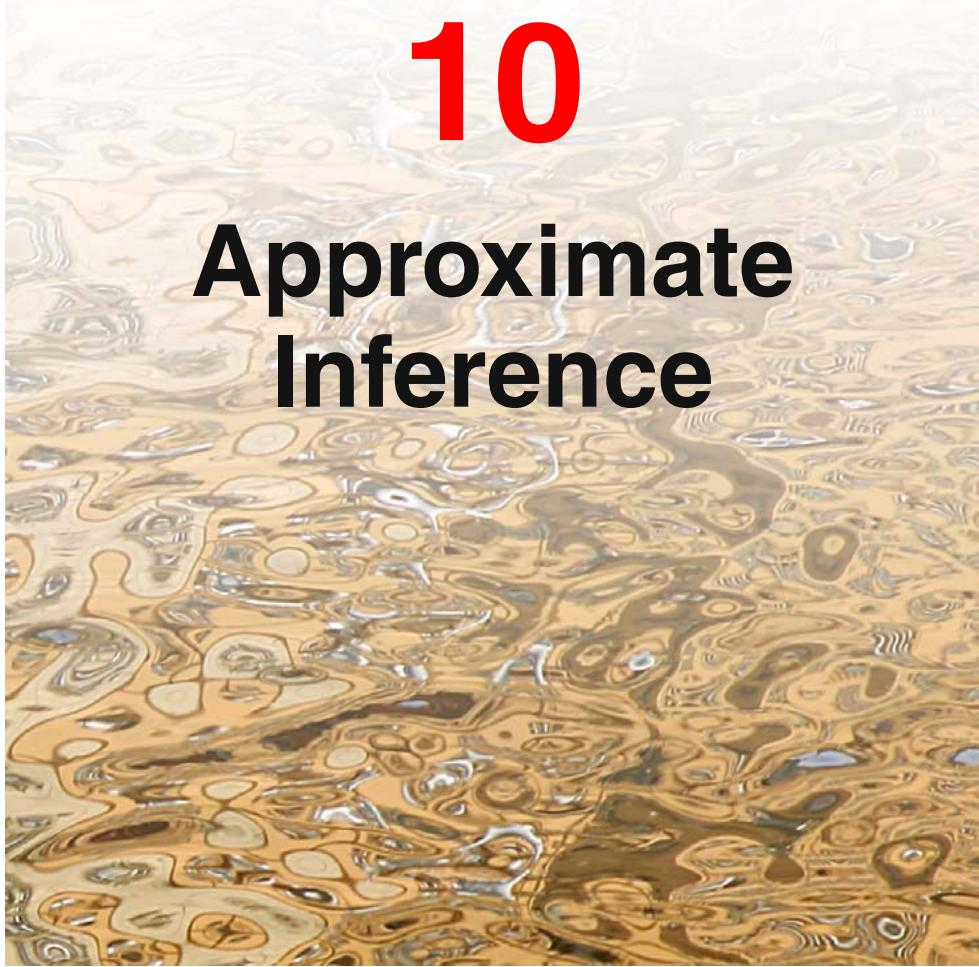
\includegraphics[keepaspectratio,alt={image}]{images/8c8af1418a8f2c9d8260c553d81e3e558da88300e45237767c2e4e2e1eec9a8b.jpg}}

A central task in the application of probabilistic models is the
evaluation of the posterior distribution p(Z X) of the latent variables
Z given the observed (visible) data variables X, and the evaluation of
expectations computed with respect to this distribution. The model might
also contain some deterministic parameters, which we will leave implicit
for the moment, or it may be a fully Bayesian model in which any unknown
parameters are given prior distributions and are absorbed into the set
of latent variables denoted by the vector Z. For instance, in the EM
algorithm we need to evaluate the expectation of the complete-data log
likelihood with respect to the posterior distribution of the latent
variables. For many models of practical interest, it will be infeasible
to evaluate the posterior distribution or indeed to compute expectations
with respect to this distribution. This could be because the
dimensionality of the latent space is too high to work with directly or
because the posterior distribution has a highly complex form for which
expectations are not analytically tractable. In the case of continuous
variables, the required integrations may not have closed-form analytical
solutions, while the dimensionality of the space and the complexity of
the integrand may prohibit numerical integration. For discrete
variables, the marginalizations involve summing over all possible
configurations of the hidden variables, and though this is always
possible in principle, we often find in practice that there may be
exponentially many hidden states so that exact calculation is
prohibitively expensive.

In such situations, we need to resort to approximation schemes, and
these fall broadly into two classes, according to whether they rely on
stochastic or deterministic approximations. Stochastic techniques such
as Markov chain Monte Carlo, described in Chapter 11, have enabled the
widespread use of Bayesian methods across many domains. They generally
have the property that given infinite computational resource, they can
generate exact results, and the approximation arises from the use of a
finite amount of processor time. In practice, sampling methods can be
computationally demanding, often limiting their use to small-scale
problems. Also, it can be difficult to know whether a sampling scheme is
generating independent samples from the required distribution.

In this chapter, we introduce a range of deterministic approximation
schemes, some of which scale well to large applications. These are based
on analytical approximations to the posterior distribution, for example
by assuming that it factorizes in a particular way or that it has a
specific parametric form such as a Gaussian. As such, they can never
generate exact results, and so their strengths and weaknesses are
complementary to those of sampling methods.

In Section 4.4, we discussed the Laplace approximation, which is based
on a local Gaussian approximation to a mode (i.e., a maximum) of the
distribution. Here we turn to a family of approximation techniques
called variational inference or variational Bayes, which use more global
criteria and which have been widely applied. We conclude with a brief
introduction to an alternative variational framework known as
expectation propagation.

\subsection{10.1. Variational Inference}\label{variational-inference}

Variational methods have their origins in the
\(1 8 ^ { \mathrm { t h } }\) century with the work of Euler, Lagrange,
and others on the calculus of variations. Standard calculus is concerned
with finding derivatives of functions. We can think of a function as a
mapping that takes the value of a variable as the input and returns the
value of the function as the output. The derivative of the function then
describes how the output value varies as we make infinitesimal changes
to the input value. Similarly, we can define a functional as a mapping
that takes a function as the input and that returns the value of the
functional as the output. An example would be the entropy
\(\mathrm { H } [ p ]\) , which takes a probability distribution
\(p ( x )\) as the input and returns the quantity

\[
\mathrm{H} [ p ] = \int p (x) \ln p (x) \mathrm{d} x\tag{10.1}
\]

as the output. We can the introduce the concept of afunctional
derivative, which expresses how the value of the functional changes in
response to infinitesimal changes to the input function (Feynman et al.,
1964). The rules for the calculus of variations mirror those of standard
calculus and are discussed in Appendix D. Many problems can be expressed
in terms of an optimization problem in which the quantity being
optimized is a functional. The solution is obtained by exploring all
possible input functions to find the one that maximizes, or minimizes,
the functional. Variational methods have broad applicability and include
such areas as finite element methods (Kapur, 1989) and maximum entropy
(Schwarz, 1988).

Although there is nothing intrinsically approximate about variational
methods, they do naturally lend themselves to finding approximate
solutions. This is done by restricting the range of functions over which
the optimization is performed, for instance by considering only
quadratic functions or by considering functions composed of a linear
combination of fixed basis functions in which only the coefficients of
the linear combination can vary. In the case of applications to
probabilistic inference, the restriction may for example take the form
of factorization assumptions (Jordan et al., 1999; Jaakkola, 2001).

Now let us consider in more detail how the concept of variational
optimization can be applied to the inference problem. Suppose we have a
fully Bayesian model in which all parameters are given prior
distributions. The model may also have latent variables as well as
parameters, and we shall denote the set of all latent variables and
parameters by \(\mathbf { Z } .\) Similarly, we denote the set of all
observed variables by X. For example, we might have a set of N
independent, identically distributed data, for which
\(\mathbf { X } ~ = ~ \{ \mathbf { x } _ { 1 } , \ldots , \mathbf { x } _ { N } \}\)
and
\(\mathbf { Z } \ = \ \{ \mathbf { z } _ { 1 } , \ldots , \mathbf { z } _ { N } \}\)
Our probabilistic model specifies the joint distribution
\(p ( \mathbf { X } , \mathbf { Z } )\) , and our goal is to find an
approximation for the posterior distribution
\(p ( \mathbf { Z } | \mathbf { X } )\) as well as for the model
evidence \(p ( \mathbf { X } )\) . As in our discussion of EM, we can
decompose the log marginal probability using

\[
\ln p (\mathbf {X}) = \mathcal {L} (q) + \mathrm{KL} (q \| p)\tag{10.2}
\]

where we have defined

\[
\mathcal {L} (q) = \int q (\mathbf {Z}) \ln \left\{\frac {p (\mathbf {X} , \mathbf {Z})}{q (\mathbf {Z})} \right\} \mathrm{d} \mathbf {Z}\tag{10.3}
\]

\[
\mathrm{KL} (q \| p) = - \int q (\mathbf {Z}) \ln \left\{\frac {p (\mathbf {Z} | \mathbf {X})}{q (\mathbf {Z})} \right\} \mathrm{d} \mathbf {Z}.\tag{10.4}
\]

This differs from our discussion of EM only in that the parameter vector
\(\pmb \theta\) no longer appears, because the parameters are now
stochastic variables and are absorbed into Z. Since in this chapter we
will mainly be interested in continuous variables we have used
integrations rather than summations in formulating this decomposition.
However, the analysis goes through unchanged if some or all of the
variables are discrete simply by replacing the integrations with
summations as required. As before, we can maximize the lower bound
\(\mathcal { L } ( q )\) by optimization with respect to the
distribution \(q ( \mathbf { Z } )\) , which is equivalent to minimizing
the KL divergence. If we allow any possible choice for
\(q ( \mathbf { Z } )\) , then the maximum of the lower bound occurs
when the KL divergence vanishes, which occurs when
\(q ( \mathbf { Z } )\) equals the posterior distribution
\(p ( \mathbf { Z } | \mathbf { X } )\)

\pandocbounded{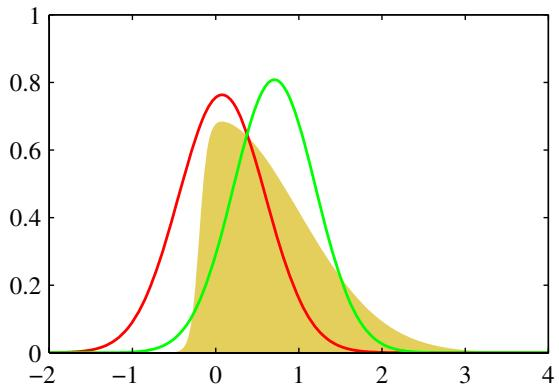
\includegraphics[keepaspectratio,alt={image}]{images/309a4195f7c93a93f4a5c88bb1ac2415be0514987b73a0603895701fc9c48309.jpg}}

\pandocbounded{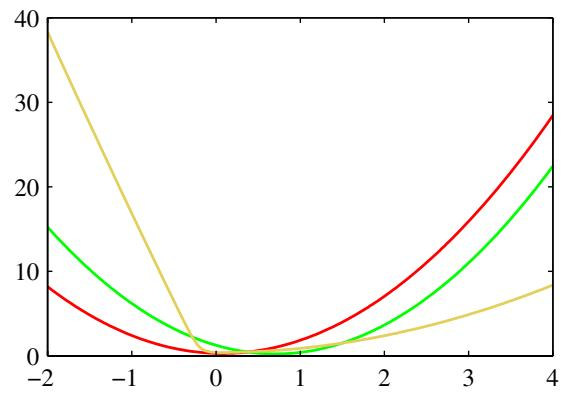
\includegraphics[keepaspectratio,alt={image}]{images/deec9a2403c4ac5357694091b8bcdc15ee24afad9f0ffb1ebd4a57ab5e3d88d8.jpg}}

Figure 10.1 Illustration of the variational approximation for the
example considered earlier in Figure 4.14. The left-hand plot shows the
original distribution (yellow) along with the Laplace (red) and
variational (green) approximations, and the right-hand plot shows the
negative logarithms of the corresponding curves.

However, we shall suppose the model is such that working with the true
posterior distribution is intractable.

We therefore consider instead a restricted family of distributions
\(q ( \mathbf { Z } )\) and then seek the member of this family for
which the KL divergence is minimized. Our goal is to restrict the family
sufficiently that they comprise only tractable distributions, while at
the same time allowing the family to be sufficiently rich and flexible
that it can provide a good approximation to the true posterior
distribution. It is important to emphasize that the restriction is
imposed purely to achieve tractability, and that subject to this
requirement we should use as rich a family of approximating
distributions as possible. In particular, there is no `over-fitting'
associated with highly flexible distributions. Using more flexible
approximations simply allows us to approach the true posterior
distribution more closely.

One way to restrict the family of approximating distributions is to use
a parametric distribution \(q ( \mathbf { Z } | \omega )\) governed by a
set of parameters \(\omega .\) . The lower bound
\(\mathcal { L } ( q )\) then becomes a function of \(\omega ,\) , and
we can exploit standard nonlinear optimization techniques to determine
the optimal values for the parameters. An example of this approach, in
which the variational distribution is a Gaussian and we have optimized
with respect to its mean and variance, is shown in Figure 10.1.

\subsection{10.1.1 Factorized
distributions}\label{factorized-distributions}

Here we consider an alternative way in which to restrict the family of
distributions \(q ( \mathbf { Z } )\) . Suppose we partition the
elements of \(\mathbf { Z }\) into disjoint groups that we denote by
\(\mathbf { Z } _ { i }\) where \(i = 1 , \dots , M\) . We then assume
that the \(q\) distribution factorizes with respect to these groups, so
that

\[
q (\mathbf {Z}) = \prod_ {i = 1} ^ {M} q _ {i} (\mathbf {Z} _ {i}).\tag{10.5}
\]

It should be emphasized that we are making no further assumptions about
the distribution. In particular, we place no restriction on the
functional forms of the individual factors
\(q _ { i } ( \mathbf { Z } _ { i } )\) . This factorized form of
variational inference corresponds to an approximation framework
developed in physics called mean field theory (Parisi, 1988).

Amongst all distributions \(q ( \mathbf { Z } )\) having the form
(10.5), we now seek that distribution for which the lower bound
\(\mathcal { L } ( q )\) is largest. We therefore wish to make a free
form (variational) optimization of \(\mathcal { L } ( q )\) with respect
to all of the distributions \(q _ { i } ( \mathbf { Z } _ { i } )\)
which we do by optimizing with respect to each of the factors in turn.
To achieve this, we first substitute (10.5) into (10.3) and then dissect
out the dependence on one of the factors
\(q _ { j } ( \mathbf { Z } _ { j } )\) . Denoting
\(q _ { j } ( \mathbf { Z } _ { j } )\) by simply \(q _ { j }\) to keep
the notation uncluttered, we then obtain

\[
\begin{array}{r c l} \mathcal {L} (q) & = & \int \prod_ {i} q _ {i} \left\{\ln p (\mathbf {X}, \mathbf {Z}) - \sum_ {i} \ln q _ {i} \right\} \mathrm{d} \mathbf {Z} \\ & = & \int q _ {j} \left\{\int \ln p (\mathbf {X}, \mathbf {Z}) \prod_ {i \neq j} q _ {i} \mathrm{d} \mathbf {Z} _ {i} \right\} \mathrm{d} \mathbf {Z} _ {j} - \int q _ {j} \ln q _ {j} \mathrm{d} \mathbf {Z} _ {j} + \text { const } \\ & = & \int q _ {j} \ln \widetilde {p} (\mathbf {X}, \mathbf {Z} _ {j})   \mathrm{d} \mathbf {Z} _ {j} - \int q _ {j} \ln q _ {j}   \mathrm{d} \mathbf {Z} _ {j} + \text { const } \end{array} \tag {10}\tag{10.6}
\]

where we have defined a new distribution
\(\widetilde { p } ( \mathbf { X } , \mathbf { Z } _ { j } )\) by the
relation

\[
\ln \widetilde {p} (\mathbf {X}, \mathbf {Z} _ {j}) = \mathbb {E} _ {i \neq j} [ \ln p (\mathbf {X}, \mathbf {Z}) ] + \text { const }.\tag{10.7}
\]

Here the notation \(\mathbb { E } _ { i \neq j } [ \cdot \cdot \cdot ]\)
denotes an expectation with respect to the q distributions over all
variables \(\mathbf { z } _ { i }\) for \(i \neq j\) , so that

\[
\mathbb {E} _ {i \neq j} [ \ln p (\mathbf {X}, \mathbf {Z}) ] = \int \ln p (\mathbf {X}, \mathbf {Z}) \prod_ {i \neq j} q _ {i} \mathrm{d} \mathbf {Z} _ {i}.\tag{10.8}
\]

Now suppose we keep the \(\{ q _ { i \neq j } \}\) fixed and maximize
\(\mathcal { L } ( q )\) in (10.6) with respect to all possible forms
for the distribution \(q _ { j } ( \mathbf { Z } _ { j } )\) . This is
easily done by recognizing that (10.6) is a negative Kullback-Leibler
divergence between \(q _ { j } ( \mathbf { Z } _ { j } )\) and
\(\widetilde { p } ( \mathbf { X } , \mathbf { Z } _ { j } )\) . Thus
maximizing (10.6) is equivalent to minimizing the Kullback-Leibler

\pandocbounded{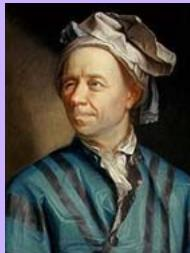
\includegraphics[keepaspectratio,alt={image}]{images/6661e37faed7df94490a443c3cad320714f45f5568d975ed4e9c2d39daf7aa38.jpg}}

\subsection{Leonhard Euler 1707--1783}\label{leonhard-euler-17071783}

Euler was a Swiss mathematician and physicist who worked in
St.~Petersburg and Berlin and who is widely considered to be one of the
greatest mathematicians of all time. He is certainly the most prolific,
and

his collected works fill 75 volumes. Amongst his many contributions, he
formulated the modern theory of the function, he developed (together
with Lagrange) the calculus of variations, and he discovered the formula
\(e ^ { i \pi } ~ = ~ - 1\) which relates four of the most important
numbers in mathematics. During the last 17 years of his life, he was
almost totally blind, and yet he produced nearly half of his results
during this period.

divergence, and the minimum occurs when
\(q _ { j } ( \mathbf { Z } _ { j } ) = \widetilde { p } ( \mathbf { X } , \mathbf { Z } _ { j } )\)
. Thus we obtain a general expression for the optimal solution
\(q _ { j } ^ { \star } ( \mathbf { Z } _ { j } )\) given by

\[
\ln q _ {j} ^ {\star} (\mathbf {Z} _ {j}) = \mathbb {E} _ {i \neq j} [ \ln p (\mathbf {X}, \mathbf {Z}) ] + \mathrm{const.}\tag{10.9}
\]

It is worth taking a few moments to study the form of this solution as
it provides the basis for applications of variational methods. It says
that the log of the optimal solution for factor \(q _ { j }\) is
obtained simply by considering the log of the joint distribution over
all hidden and visible variables and then taking the expectation with
respect to all of the other factors \(\{ q _ { i } \}\) for \(i \neq j\)

The additive constant in (10.9) is set by normalizing the distribution
\(q _ { j } ^ { \star } ( \mathbf { Z } _ { j } )\) Thus if we take the
exponential of both sides and normalize, we have

\[
q _ {j} ^ {\star} (\mathbf {Z} _ {j}) = \frac {\exp \left(\mathbb {E} _ {i \neq j} [ \ln p (\mathbf {X} , \mathbf {Z}) ]\right)}{\int \exp \left(\mathbb {E} _ {i \neq j} [ \ln p (\mathbf {X} , \mathbf {Z}) ]\right) \mathrm{d} \mathbf {Z} _ {j}}.
\]

In practice, we shall find it more convenient to work with the form
(10.9) and then reinstate the normalization constant (where required) by
inspection. This will become clear from subsequent examples.

The set of equations given by (10.9) for \(j = 1 , \dots , M\) represent
a set of consistency conditions for the maximum of the lower bound
subject to the factorization constraint. However, they do not represent
an explicit solution because the expression on the right-hand side of
(10.9) for the optimum
\(q _ { j } ^ { \star } ( \mathbf { Z } _ { j } )\) depends on
expectations computed with respect to the other factors
\(q _ { i } ( \mathbf { Z } _ { i } )\) for \(i \neq j\) . We will
therefore seek a consistent solution by first initializing all of the
factors \(q _ { i } ( \mathbf { Z } _ { i } )\) appropriately and then
cycling through the factors and replacing each in turn with a revised
estimate given by the right-hand side of (10.9) evaluated using the
current estimates for all of the other factors. Convergence is
guaranteed because bound is convex with respect to each of the factors
\(q _ { i } ( \mathbf { Z } _ { i } )\) (Boyd and Vandenberghe, 2004).

\subsection{10.1.2 Properties of factorized
approximations}\label{properties-of-factorized-approximations}

Our approach to variational inference is based on a factorized
approximation to the true posterior distribution. Let us consider for a
moment the problem of approximating a general distribution by a
factorized distribution. To begin with, we discuss the problem of
approximating a Gaussian distribution using a factorized Gaussian, which
will provide useful insight into the types of inaccuracy introduced in
using factorized approximations. Consider a Gaussian distribution
\(\dot { p } ( { \bf z } ) = \mathcal { N } ( { \bf z } | \pmb { \mu } , \pmb { \Lambda } ^ { - 1 } )\)
over two correlated variables
\(\textbf { z } = \ ( z _ { 1 } , z _ { 2 } )\) in which the mean and
precision have elements

\[
\boldsymbol {\mu} = \binom{\mu_ {1}}{\mu_ {2}}, \qquad \boldsymbol {\Lambda} = \left( \begin{array}{c c} \Lambda_ {1 1} & \Lambda_ {1 2} \\ \Lambda_ {2 1} & \Lambda_ {2 2} \end{array} \right)\tag{10.10}
\]

and \(\Lambda _ { 2 1 } = \Lambda _ { 1 2 }\) due to the symmetry of the
precision matrix. Now suppose we wish to approximate this distribution
using a factorized Gaussian of the form \(q ( \mathbf { z } ) =\)
\(q _ { 1 } ( z _ { 1 } ) q _ { 2 } ( z _ { 2 } )\) . We first apply the
general result (10.9) to find an expression for the optimal factor
\(q _ { 1 } ^ { \star } ( z _ { 1 } )\) . In doing so it is useful to
note that on the right-hand side we only need to retain those terms that
have some functional dependence on \(z _ { 1 }\) because all other terms
can be absorbed into the normalization constant. Thus we have

\[
\begin{array}{r c l} \ln q _ {1} ^ {\star} (z _ {1}) & = & \mathbb {E} _ {z _ {2}} [ \ln p (\mathbf {z}) ] + \text { const } \\ & = & \mathbb {E} _ {z _ {2}} \left[ - \frac {1}{2} (z _ {1} - \mu_ {1}) ^ {2} \Lambda_ {1 1} - (z _ {1} - \mu_ {1}) \Lambda_ {1 2} (z _ {2} - \mu_ {2}) \right] + \text { const } \\ & = & - \frac {1}{2} z _ {1} ^ {2} \Lambda_ {1 1} + z _ {1} \mu_ {1} \Lambda_ {1 1} - z _ {1} \Lambda_ {1 2} (\mathbb {E} [ z _ {2} ] - \mu_ {2}) + \text { const }. \end{array} \tag {10.}\tag{10.11}
\]

Next we observe that the right-hand side of this expression is a
quadratic function of \(z _ { 1 }\) , and so we can identify
\(q ^ { \star } ( z _ { 1 } )\) as a Gaussian distribution. It is worth
emphasizing that we did not assume that \(q ( z _ { i } )\) is Gaussian,
but rather we derived this result by variational optimization of the KL
divergence over all possible distributions \(q ( z _ { i } )\) Note also
that we do not need to consider the additive constant in (10.9)
explicitly because it represents the normalization constant that can be
found at the end by inspection if required. Using the technique of
completing the square, we can identify the mean and precision of this
Gaussian, giving

Section 2.3.1

\[
q ^ {\star} (z _ {1}) = \mathcal {N} (z _ {1} | m _ {1}, \Lambda_ {1 1} ^ {- 1})\tag{10.12}
\]

where

\[
m _ {1} = \mu_ {1} - \Lambda_ {1 1} ^ {- 1} \Lambda_ {1 2} \left(\mathbb {E} [ z _ {2} ] - \mu_ {2}\right).\tag{10.13}
\]

By symmetry, \(q _ { 2 } ^ { \star } ( z _ { 2 } )\) is also Gaussian
and can be written as

\[
q _ {2} ^ {\star} (z _ {2}) = \mathcal {N} (z _ {2} | m _ {2}, \Lambda_ {2 2} ^ {- 1})\tag{10.14}
\]

in which

\[
m _ {2} = \mu_ {2} - \Lambda_ {2 2} ^ {- 1} \Lambda_ {2 1} \left(\mathbb {E} [ z _ {1} ] - \mu_ {1}\right).\tag{10.15}
\]

Note that these solutions are coupled, so that
\(q ^ { \star } ( z _ { 1 } )\) depends on expectations computed with
respect to \(q ^ { \star } ( z _ { 2 } )\) and vice versa. In general,
we address this by treating the variational solutions as re-estimation
equations and cycling through the variables in turn updating them until
some convergence criterion is satisfied. We shall see an example of this
shortly. Here, however, we note that the problem is sufficiently simple
that a closed form solution can be found. In particular, because
\(\mathbb { E } [ z _ { 1 } ] = m _ { 1 }\) and
\(\mathbb { E } [ z _ { 2 } ] = m _ { 2 }\) , we see that the two
equations are satisfied if we take
\(\mathbb { E } [ z _ { 1 } ] = \mu _ { 1 }\) and
\(\mathbb { E } [ z _ { 2 } ] = \mu _ { 2 }\) , and it is easily shown
that this is the only solution provided the distribution is nonsingular.
This result is illustrated in Figure 10.2(a). We see that the mean is
correctly captured but that the variance of \(q ( \mathbf { z } )\) is
controlled by the direction of smallest variance of
\(p ( \mathbf { z } )\) , and that the variance along the orthogonal
direction is significantly under-estimated. It is a general result that
a factorized variational approximation tends to give approximations to
the posterior distribution that are too compact.

By way of comparison, suppose instead that we had been minimizing the
reverse Kullback-Leibler divergence \(\mathrm { K L } ( p | | q )\) . As
we shall see, this form of KL divergence

Figure 10.2 Comparison of the two alternative forms for the
Kullback-Leibler divergence. The green contours corresponding to 1, 2,
and 3 standard deviations for a correlated Gaussian distribution
\(p ( \mathbf { z } )\) over two variables \(z _ { 1 }\) and
\(z _ { 2 }\) and the red contours represent the corresponding levels
for an approximating distribution \(q ( \mathbf { z } )\) over the same
variables given by the product of two independent univariate Gaussian
distributions whose parameters are obtained by minimization of (a) the
Kullback-Leibler divergence \(\mathrm { K L } ( q \| p )\) and (b) the
reverse Kullback-Leibler divergence \(\mathrm { K L } ( p | | q )\)

\pandocbounded{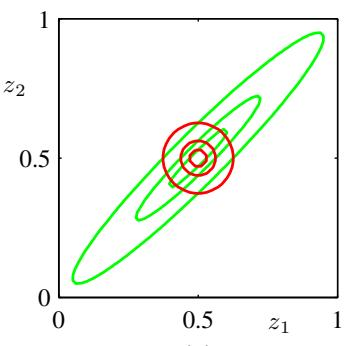
\includegraphics[keepaspectratio,alt={image}]{images/107540168c71c12cea907b9287cd23807201a71ebe92d6bad2b4eb43d9af1951.jpg}}

\begin{enumerate}
\def\labelenumi{(\alph{enumi})}
\tightlist
\item
\end{enumerate}

\pandocbounded{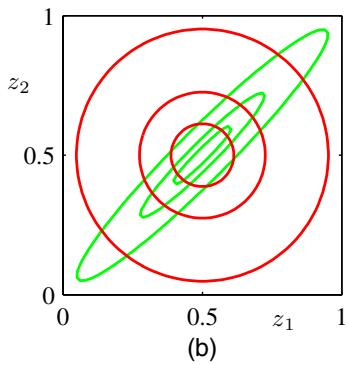
\includegraphics[keepaspectratio,alt={image}]{images/3689725d7e1ce1f627f5be297bc0f74914cf02681c15d793bd21be3e3c0e8c70.jpg}}

Section 10.7

is used in an alternative approximate inference framework called
expectation propagation. We therefore consider the general problem of
minimizing KL \(( p \| q )\) when \(q ( \mathbf { Z } )\) is a
factorized approximation of the form (10.5). The KL divergence can then
be written in the form

\[
\mathrm{KL} (p \| q) = - \int p (\mathbf {Z}) \left[ \sum_ {i = 1} ^ {M} \ln q _ {i} (\mathbf {Z} _ {i}) \right] \mathrm{d} \mathbf {Z} + \mathrm{const}\tag{10.16}
\]

Exercise 10.3

where the constant term is simply the entropy of \(p ( \mathbf { Z } )\)
and so does not depend on \(q ( \mathbf { Z } )\) . We can now optimize
with respect to each of the factors
\(q _ { j } ( \mathbf { Z } _ { j } )\) , which is easily done using a
Lagrange multiplier to give

\[
q _ {j} ^ {\star} (\mathbf {Z} _ {j}) = \int p (\mathbf {Z}) \prod_ {i \neq j} \mathrm{d} \mathbf {Z} _ {i} = p (\mathbf {Z} _ {j}).\tag{10.17}
\]

In this case, we find that the optimal solution for
\(q _ { j } ( \mathbf { Z } _ { j } )\) is just given by the
corresponding marginal distribution of \(p ( \mathbf { Z } )\) . Note
that this is a closed-form solution and so does not require iteration.

To apply this result to the illustrative example of a Gaussian
distribution \(p ( \mathbf { z } )\) over a vector z we can use (2.98),
which gives the result shown in Figure 10.2(b). We see that once again
the mean of the approximation is correct, but that it places significant
probability mass in regions of variable space that have very low
probability.

The difference between these two results can be understood by noting
that there is a large positive contribution to the Kullback-Leibler
divergence

\[
\mathrm{KL} (q \| p) = - \int q (\mathbf {Z}) \ln \left\{\frac {p (\mathbf {Z})}{q (\mathbf {Z})} \right\} \mathrm{d} \mathbf {Z}\tag{10.18}
\]

\begin{enumerate}
\def\labelenumi{(\alph{enumi})}
\setcounter{enumi}{2}
\tightlist
\item
\end{enumerate}

\pandocbounded{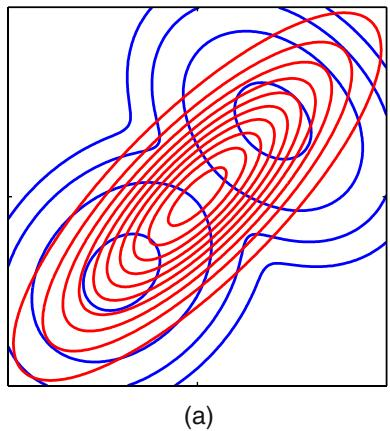
\includegraphics[keepaspectratio,alt={image}]{images/f77bef3060afa3db6357905249388fc5ee47c653f9709a762b0845c0cc178adb.jpg}}

\pandocbounded{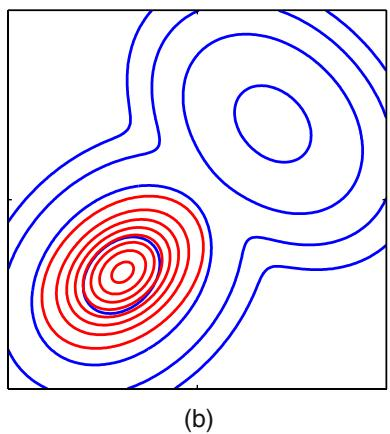
\includegraphics[keepaspectratio,alt={image}]{images/9d6817463717df792b7619f52af37c3dd6ba45031547ae311c0b33e1148d035b.jpg}}

\pandocbounded{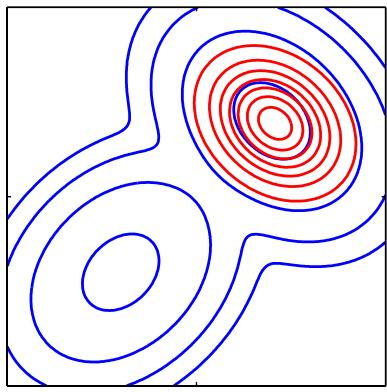
\includegraphics[keepaspectratio,alt={image}]{images/d4aac4fccd14c4e313db53d81daeac84fd25c627941fdc418dfaf0621c4e92bb.jpg}}

Figure 10.3 Another comparison of the two alternative forms for the
Kullback-Leibler divergence. (a) The blue contours show a bimodal
distribution \(p ( \mathbf { Z } )\) given by a mixture of two
Gaussians, and the red contours correspond to the single Gaussian
distribution \(q ( \mathbf { Z } )\) that best approximates
\(p ( \mathbf { Z } )\) in the sense of minimizing the Kullback-Leibler
divergence \(\mathrm { K L } ( p | | q )\) . (b)
\(\mathsf { A } \mathsf { s }\) in (a) but now the red contours
correspond to a Gaussian distribution \(q ( \mathbf { Z } )\) found by
numerical minimization of the Kullback-Leibler divergence KL
\(( q \| p )\) . (c) As in (b) but showing a different local minimum of
the Kullback-Leibler divergence.

from regions of Z space in which \(p ( \mathbf { Z } )\) is near zero
unless \(q ( \mathbf { Z } )\) is also close to zero. Thus minimizing
this form of KL divergence leads to distributions
\(q ( \mathbf { Z } )\) that avoid regions in which
\(p ( \mathbf { Z } )\) is small. Conversely, the Kullback-Leibler
divergence KL \(( p \| q )\) is minimized by distributions
\(q ( \mathbf { Z } )\) that are nonzero in regions where
\(p ( \mathbf { Z } )\) is nonzero.

We can gain further insight into the different behaviour of the two KL
divergences if we consider approximating a multimodal distribution by a
unimodal one, as illustrated in Figure 10.3. In practical applications,
the true posterior distribution will often be multimodal, with most of
the posterior mass concentrated in some number of relatively small
regions of parameter space. These multiple modes may arise through
nonidentifiability in the latent space or through complex nonlinear
dependence on the parameters. Both types of multimodality were
encountered in Chapter 9 in the context of Gaussian mixtures, where they
manifested themselves as multiple maxima in the likelihood function, and
a variational treatment based on the minimization of
\(\mathrm { K L } ( q \| p )\) will tend to find one of these modes. By
contrast, if we were to minimize \(\mathrm { K L } ( p | | q )\) , the
resulting approximations would average across all of the modes and, in
the context of the mixture model, would lead to poor predictive
distributions (because the average of two good parameter values is
typically itself not a good parameter value). It is possible to make use
of \(\mathrm { K L } ( p | | q )\) to define a useful inference
procedure, but this requires a rather different approach to the one
discussed here, and will be considered in detail when we discuss
expectation propagation.

The two forms of Kullback-Leibler divergence are members of the alpha
family

of divergences (Ali and Silvey, 1966; Amari, 1985; Minka, 2005) defined
by

\[
\mathrm{D} _ {\alpha} (p \| q) = \frac {4}{1 - \alpha^ {2}} \left(1 - \int p (x) ^ {(1 + \alpha) / 2} q (x) ^ {(1 - \alpha) / 2} \mathrm{d} x\right)\tag{10.19}
\]

where \(- \infty < \alpha < \infty\) is a continuous parameter. The
Kullback-Leibler divergence \(\mathrm { K L } ( p | | q )\) corresponds
to the limit \(\alpha  1\) , whereas \(\mathrm { K L } ( q \| p )\)
corresponds to the limit \(\alpha  - 1\) . For all values of α we have
\(\begin{array} { r } { \mathrm { D } _ { \alpha } ( p \Vert q ) \geqslant 0 } \end{array}\)
, with equality if, and only if, \(p ( x ) = q ( x )\) . Suppose
\(p ( x )\) is a fixed distribution, and we minimize
\(\mathrm { D } _ { \alpha } ( p \Vert q )\) with respect to some set of
distributions \(q ( x )\) . Then for \(\alpha \leqslant - 1\) the
divergence is zero forcing, so that any values of x for which
\(p ( x ) = 0\) will have \(q ( x ) = 0\) , and typically \(q ( x )\)
will under-estimate the support of \(p ( x )\) and will tend to seek the
mode with the largest mass. Conversely for \(\alpha \geqslant 1\) the
divergence is zero-avoiding, so that values of \(x\) for which
\(p ( x ) > 0\) will have \(q ( x ) > 0\) , and typically \(q ( x )\)
will stretch to cover all of \(p ( x )\) , and will over-estimate the
support of \(p ( x )\) . When \(\alpha = 0\) we obtain a symmetric
divergence that is linearly related to the Hellinger distance given by

\[
\mathrm{D} _ {\mathrm{H}} (p \| q) = \int \left(p (x) ^ {1 / 2} - q (x) ^ {1 / 2}\right) \mathrm{d} x.\tag{10.20}
\]

The square root of the Hellinger distance is a valid distance metric.

\subsection{10.1.3 Example: The univariate
Gaussian}\label{example-the-univariate-gaussian}

We now illustrate the factorized variational approximation using a
Gaussian distribution over a single variable x (MacKay, 2003). Our goal
is to infer the posterior distribution for the mean \(\mu\) and
precision \(\tau ,\) given a data set
\(\mathcal { D } = \{ x _ { 1 } , \ldots , x _ { N } \}\) of observed
values of \(x\) which are assumed to be drawn independently from the
Gaussian. The likelihood function is given by

\[
p (\mathcal {D} | \mu , \tau) = \left(\frac {\tau}{2 \pi}\right) ^ {N / 2} \exp \left\{- \frac {\tau}{2} \sum_ {n = 1} ^ {N} (x _ {n} - \mu) ^ {2} \right\}.\tag{10.21}
\]

We now introduce conjugate prior distributions for \(\mu\) and \(\tau\)
given by

\[
p (\mu | \tau) = \mathcal {N} \left(\mu | \mu_ {0}, (\lambda_ {0} \tau) ^ {- 1}\right)\tag{10.22}
\]

\[
{p (\tau)} = {\mathrm{Gam} (\tau | a _ {0}, b _ {0})}\tag{10.23}
\]

where Gam \(( \tau | a _ { 0 } , b _ { 0 } )\) is the gamma distribution
defined by (2.146). Together these distributions constitute a
Gaussian-Gamma conjugate prior distribution.

For this simple problem the posterior distribution can be found exactly,
and again takes the form of a Gaussian-gamma distribution. However, for
tutorial purposes we will consider a factorized variational
approximation to the posterior distribution given by

\[
q (\mu , \tau) = q _ {\mu} (\mu) q _ {\tau} (\tau).\tag{10.24}
\]

Note that the true posterior distribution does not factorize in this
way. The optimum factors \(q _ { \mu } ( \mu )\) and
\(q _ { \tau } ( \tau )\) can be obtained from the general result (10.9)
as follows. For \(q _ { \mu } ( \mu )\) we have

\[
\begin{array}{r c l} \ln q _ {\mu} ^ {\star} (\mu) & = & \mathbb {E} _ {\tau} \left[ \ln p (\mathcal {D} | \mu , \tau) + \ln p (\mu | \tau) \right] + \text { const } \\ & = & - \frac {\mathbb {E} [ \tau ]}{2} \left\{\lambda_ {0} (\mu - \mu_ {0}) ^ {2} + \sum_ {n = 1} ^ {N} (x _ {n} - \mu) ^ {2} \right\} + \text { const }. \end{array}\tag{10.25}
\]

Completing the square over \(\mu\) we see that \(q _ { \mu } ( \mu )\)
is a Gaussian
\(\mathcal { N } \left( \mu \vert \mu _ { N } , \lambda _ { N } ^ { - 1 } \right)\)
with mean and precision given by

\[
\mu_ {N} = \frac {\lambda_ {0} \mu_ {0} + N \overline {{x}}}{\lambda_ {0} + N}\tag{10.26}
\]

\[
\lambda_ {N} = (\lambda_ {0} + N) \mathbb {E} [ \tau ].\tag{10.27}
\]

Note that for \(N  \infty\) this gives the maximum likelihood result in
which \(\mu _ { N } = \overline { { x } }\) and the precision is
infinite.

Similarly, the optimal solution for the factor \(q _ { \tau } ( \tau )\)
is given by

\[
\begin{array}{r c l} \ln q _ {\tau} ^ {\star} (\tau) & = & \mathbb {E} _ {\mu} \left[ \ln p (\mathcal {D} | \mu , \tau) + \ln p (\mu | \tau) \right] + \ln p (\tau) + \text { const } \\ & = & (a _ {0} - 1) \ln \tau - b _ {0} \tau + \frac {N}{2} \ln \tau \\ & & - \frac {\tau}{2} \mathbb {E} _ {\mu} \left[ \sum_ {n = 1} ^ {N} (x _ {n} - \mu) ^ {2} + \lambda_ {0} (\mu - \mu_ {0}) ^ {2} \right] + \text { const } \end{array}\tag{10.28}
\]

and hence \(q _ { \tau } ( \tau )\) is a gamma distribution
\({ \mathrm { G a m } } ( \tau | a _ { N } , b _ { N } )\) with
parameters

\[
a _ {N} = a _ {0} + \frac {N}{2}\tag{10.29}
\]

\[
{b _ {N}} = {b _ {0} + \frac {1}{2} \mathbb {E} _ {\mu} \left[ \sum_ {n = 1} ^ {N} (x _ {n} - \mu) ^ {2} + \lambda_ {0} (\mu - \mu_ {0}) ^ {2} \right].}\tag{10.30}
\]

Again this exhibits the expected behaviour when \(N \to \infty\)

It should be emphasized that we did not assume these specific functional
forms for the optimal distributions \(q _ { \mu } ( \mu )\) and
\(q _ { \tau } ( \tau )\) . They arose naturally from the structure of
the likelihood function and the corresponding conjugate priors.

Thus we have expressions for the optimal distributions
\(q _ { \mu } ( \mu )\) and \(q _ { \tau } ( \tau )\) each of which
depends on moments evaluated with respect to the other distribution. One
approach to finding a solution is therefore to make an initial guess
for, say, the moment \(\mathbb { E } [ \tau ]\) and use this to
re-compute the distribution \(q _ { \mu } ( \mu )\) . Given this revised
distribution we can then extract the required moments
\(\mathbb { E } [ \mu ]\) and \(\mathbb { E } [ \mu ^ { 2 } ]\) , and
use these to recompute the distribution \(q _ { \tau } ( \tau )\) , and
so on. Since the space of hidden variables for this example is only two
dimensional, we can illustrate the variational approximation to the
posterior distribution by plotting contours of both the true posterior
and the factorized approximation, as illustrated in Figure 10.4.

\pandocbounded{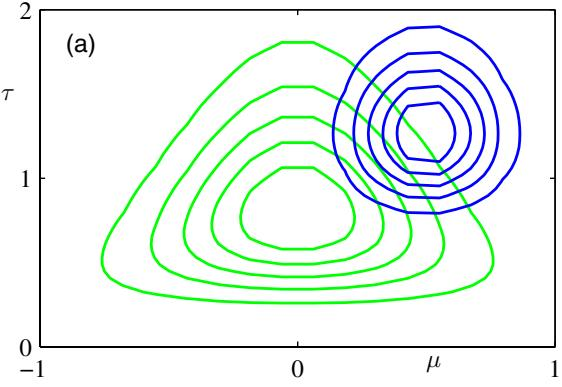
\includegraphics[keepaspectratio,alt={image}]{images/b0baed0e03d86b94eab763bb25d81813f4d22776ce80c2226ec2935caf34e7d5.jpg}}

\pandocbounded{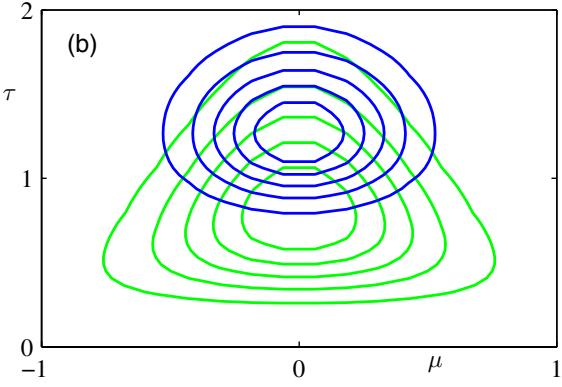
\includegraphics[keepaspectratio,alt={image}]{images/2c0f5805b78297ff5eb8df15b0b42a2903d1cc779edf8fef6a33e675fbe329f5.jpg}}

\pandocbounded{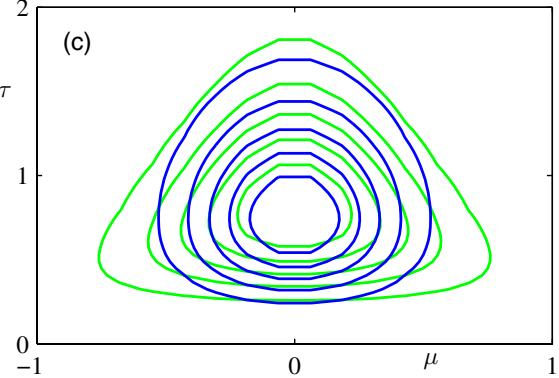
\includegraphics[keepaspectratio,alt={image}]{images/b8c9c2cdf9a1902bed4d8331e6b26b0c55e189a1ade4acd40701f519b50ab774.jpg}}

\pandocbounded{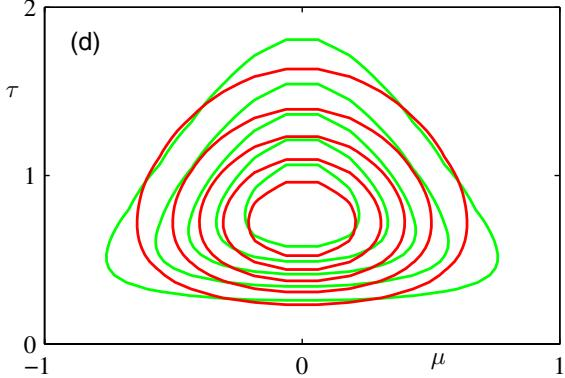
\includegraphics[keepaspectratio,alt={image}]{images/05d593b76c5e6872f8fd4b0a60ff8daa534d7c63e6667a860779be2053d9b256.jpg}}

Figure 10.4 Illustration of variational inference for the mean \(\mu\)
and precision τ of a univariate Gaussian distribu tion. Contours of the
true posterior distribution \(p ( \mu , \tau | D )\) are shown in green.
(a) Contours of the initial factorized approximation
\(q _ { \mu } ( \mu ) q _ { \tau } ( \tau )\) are shown in blue. (b)
After re-estimating the factor \(q _ { \mu } ( \mu )\) . (c) After
re-estimating the factor \(q _ { \tau } ( \tau )\) . (d) Contours of the
optimal factorized approximation, to which the iterative scheme
converges, are shown in red.

In general, we will need to use an iterative approach such as this in
order to solve for the optimal factorized posterior distribution. For
the very simple example we are considering here, however, we can find an
explicit solution by solving the simultaneous equations for the optimal
factors \(q _ { \mu } ( \mu )\) and \(q _ { \tau } ( \tau )\) . Before
doing this, we can simplify these expressions by considering broad,
noninformative priors in which
\(\mu _ { 0 } = a _ { 0 } = b _ { 0 } = \lambda _ { 0 } = 0\) . Although
these parameter settings correspond to improper priors, we see that the
posterior distribution is still well defined. Using the standard result
\(\mathbb { E } [ \tau ] = a _ { N } / b _ { N }\) for the mean of a
gamma distribution, together with (10.29) and (10.30), we have

\[
\frac {1}{\mathbb {E} [ \tau ]} = \mathbb {E} \left[ \frac {1}{N} \sum_ {n = 1} ^ {N} (x _ {n} - \mu) ^ {2} \right] = \overline {{x ^ {2}}} - 2 \overline {{x}} \mathbb {E} [ \mu ] + \mathbb {E} [ \mu^ {2} ].\tag{10.31}
\]

Then, using (10.26) and (10.27), we obtain the first and second order
moments of

\(q _ { \mu } ( \mu )\) in the form

\[
\mathbb {E} [ \mu ] = \overline {{x}}, \qquad \mathbb {E} [ \mu^ {2} ] = \overline {{x}} ^ {2} + \frac {1}{N \mathbb {E} [ \tau ]}.\tag{10.32}
\]

We can now substitute these moments into (10.31) and then solve for
\(\mathbb { E } [ \tau ]\) to give

\[
\begin{array}{r c l} \frac {1}{\mathbb {E} [ \tau ]} & = & \frac {1}{N - 1} (\overline {{x ^ {2}}} - \overline {{x}} ^ {2}) \\ & = & \frac {1}{N - 1} \sum_ {n = 1} ^ {N} (x _ {n} - \overline {{x}}) ^ {2}. \end{array}\tag{10.33}
\]

We recognize the right-hand side as the familiar unbiased estimator for
the variance of a univariate Gaussian distribution, and so we see that
the use of a Bayesian approach has avoided the bias of the maximum
likelihood solution.

\subsection{10.1.4 Model comparison}\label{model-comparison}

As well as performing inference over the hidden variables Z, we may also
wish to compare a set of candidate models, labelled by the index m, and
having prior probabilities \(p ( m )\) . Our goal is then to approximate
the posterior probabilities \(p ( m | \mathbf { X } )\) , where X is the
observed data. This is a slightly more complex situation than that
considered so far because different models may have different structure
and indeed different dimensionality for the hidden variables Z. We
cannot therefore simply consider a factorized approximation
\(q ( \mathbf { Z } ) q ( m )\) , but must instead recognize that the
posterior over Z must be conditioned on m, and so we must consider
\(q ( \mathbf { Z } , m ) = q ( \mathbf { Z } | m ) q ( m )\) . We can
readily verify the following decomposition based on this variational
distribution

\[
\ln p (\mathbf {X}) = \mathcal {L} _ {m} - \sum_ {m} \sum_ {\mathbf {Z}} q (\mathbf {Z} | m) q (m) \ln \left\{\frac {p (\mathbf {Z} , m | \mathbf {X})}{q (\mathbf {Z} | m) q (m)} \right\}\tag{10.34}
\]

where the \({ \mathcal { L } } _ { m }\) is a lower bound on ln
\(p ( \mathbf { X } )\) and is given by

\[
\mathcal {L} _ {m} = \sum_ {m} \sum_ {\mathbf {Z}} q (\mathbf {Z} | m) q (m) \ln \left\{\frac {p (\mathbf {Z} , \mathbf {X} , m)}{q (\mathbf {Z} | m) q (m)} \right\}.\tag{10.35}
\]

Here we are assuming discrete Z, but the same analysis applies to
continuous latent variables provided the summations are replaced with
integrations. We can maximize \({ \mathcal { L } } _ { m }\) with
respect to the distribution \(q ( m )\) using a Lagrange multiplier,
with the result

\[
q (m) \propto p (m) \exp \{\mathcal {L} _ {m} \}.\tag{10.36}
\]

However, if we maximize \({ \mathcal { L } } _ { m }\) with respect to
the \(q ( \mathbf { Z } | m )\) , we find that the solutions for
different m are coupled, as we expect because they are conditioned on m.
We proceed instead by first optimizing each of the
\(q ( \mathbf { Z } | m )\) individually by optimization of (10.35), and
then subsequently determining the \(q ( m )\) using (10.36). After
normalization the resulting values for \(q ( m )\) can be used for model
selection or model averaging in the usual way.

\subsection{10.2. Illustration: Variational Mixture of
Gaussians}\label{illustration-variational-mixture-of-gaussians}

We now return to our discussion of the Gaussian mixture model and apply
the variational inference machinery developed in the previous section.
This will provide a good illustration of the application of variational
methods and will also demonstrate how a Bayesian treatment elegantly
resolves many of the difficulties associated with the maximum likelihood
approach (Attias, 1999b). The reader is encouraged to work through this
example in detail as it provides many insights into the practical
application of variational methods. Many Bayesian models, corresponding
to much more sophisticated distributions, can be solved by
straightforward extensions and generalizations of this analysis.

Our starting point is the likelihood function for the Gaussian mixture
model, illustrated by the graphical model in Figure 9.6. For each
observation \({ \bf x } _ { n }\) we have a corresponding latent
variable \(\mathbf { z } _ { n }\) comprising a 1-of-K binary vector
with elements \(z _ { n k }\) for \(k = 1 , \ldots , K\) . As before we
denote the observed data set by \(\mathbf { X } =\)
\(\{ \mathbf { x } _ { 1 } , \hdots , \mathbf { x } _ { N } \}\) , and
similarly we denote the latent variables by
\(\mathbf { Z } = \{ \mathbf { z } _ { 1 } , \dotsc , \mathbf { z } _ { N } \}\)
From (9.10) we can write down the conditional distribution of
\(\mathbf { Z } ,\) given the mixing coefficients π, in the form

\[
p (\mathbf {Z} | \boldsymbol {\pi}) = \prod_ {n = 1} ^ {N} \prod_ {k = 1} ^ {K} \pi_ {k} ^ {z _ {n k}}.\tag{10.37}
\]

Similarly, from (9.11), we can write down the conditional distribution
of the observed data vectors, given the latent variables and the
component parameters

\[
p (\mathbf {X} | \mathbf {Z}, \boldsymbol {\mu}, \boldsymbol {\Lambda}) = \prod_ {n = 1} ^ {N} \prod_ {k = 1} ^ {K} \mathcal {N} \left(\mathbf {x} _ {n} | \boldsymbol {\mu} _ {k}, \boldsymbol {\Lambda} _ {k} ^ {- 1}\right) ^ {z _ {n k}}\tag{10.38}
\]

where \(\boldsymbol { \mu } = \{ \mu _ { k } \}\) and
\(\pmb { \Lambda } = \{ \pmb { \Lambda } _ { k } \}\) . Note that we are
working in terms of precision matrices rather than covariance matrices
as this somewhat simplifies the mathematics.

Next we introduce priors over the parameters \(\mu ,\) Λ and \(\pi\) .
The analysis is considerably simplified if we use conjugate prior
distributions. We therefore choose a Dirichlet distribution over the
mixing coefficients π

\[
p (\boldsymbol {\pi}) = \operatorname{Dir} (\boldsymbol {\pi} | \boldsymbol {\alpha} _ {0}) = C (\boldsymbol {\alpha} _ {0}) \prod_ {k = 1} ^ {K} \pi_ {k} ^ {\alpha_ {0} - 1}\tag{10.39}
\]

where by symmetry we have chosen the same parameter \(\alpha _ { 0 }\)
for each of the components, and \(C ( \alpha _ { 0 } )\) is the
normalization constant for the Dirichlet distribution defined

Figure 10.5 Directed acyclic graph representing the Bayesian mixture of
Gaussians model, in which the box (plate) denotes a set of N i.i.d.
observations. Here \(\mu\) denotes \(\{ \mu _ { k } \}\) and Λ denotes
\(\{ \pmb { \Lambda } _ { k } \}\)

\pandocbounded{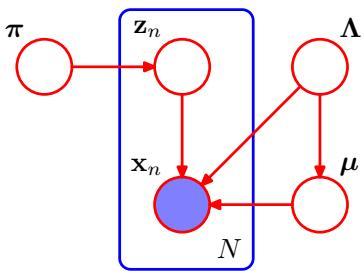
\includegraphics[keepaspectratio,alt={image}]{images/cd450ac645fd6f87839c2882e4feb95d1d720161912915eb3eee9c1f225ec406.jpg}}

by (B.23). As we have seen, the parameter \(\alpha _ { 0 }\) can be
interpreted as the effective prior number of observations associated
with each component of the mixture. If the value of \(\alpha _ { 0 }\)
is small, then the posterior distribution will be influenced primarily
by the data rather than by the prior.

Similarly, we introduce an independent Gaussian-Wishart prior governing
the mean and precision of each Gaussian component, given by

\[
\begin{array}{r c l} p (\boldsymbol {\mu}, \boldsymbol {\Lambda}) & = & p (\boldsymbol {\mu} | \boldsymbol {\Lambda}) p (\boldsymbol {\Lambda}) \\ & = & \prod_ {k = 1} ^ {K} \mathcal {N} \left(\boldsymbol {\mu} _ {k} | \mathbf {m} _ {0}, (\beta_ {0} \boldsymbol {\Lambda} _ {k}) ^ {- 1}\right) \mathcal {W} (\boldsymbol {\Lambda} _ {k} | \mathbf {W} _ {0}, \nu_ {0}) \end{array}\tag{10.40}
\]

because this represents the conjugate prior distribution when both the
mean and precision are unknown. Typically we would choose
\(\mathbf { m } _ { 0 } = \mathbf { 0 }\) by symmetry.

The resulting model can be represented as a directed graph as shown in
Figure 10.5. Note that there is a link from Λ to \(\pmb { \mu }\) since
the variance of the distribution over \(\pmb { \mu }\) in (10.40) is a
function of Λ.

This example provides a nice illustration of the distinction between
latent variables and parameters. Variables such as
\(\mathbf { z } _ { n }\) that appear inside the plate are regarded as
latent variables because the number of such variables grows with the
size of the data set. By contrast, variables such as \(\pmb { \mu }\)
that are outside the plate are fixed in number independently of the size
of the data set, and so are regarded as parameters. From the perspective
of graphical models, however, there is really no fundamental difference
between them.

\subsection{10.2.1 Variational
distribution}\label{variational-distribution}

In order to formulate a variational treatment of this model, we next
write down the joint distribution of all of the random variables, which
is given by

\[
p (\mathbf {X}, \mathbf {Z}, \boldsymbol {\pi}, \boldsymbol {\mu}, \boldsymbol {\Lambda}) = p (\mathbf {X} | \mathbf {Z}, \boldsymbol {\mu}, \boldsymbol {\Lambda}) p (\mathbf {Z} | \boldsymbol {\pi}) p (\boldsymbol {\pi}) p (\boldsymbol {\mu} | \boldsymbol {\Lambda}) p (\boldsymbol {\Lambda})\tag{10.41}
\]

in which the various factors are defined above. The reader should take a
moment to verify that this decomposition does indeed correspond to the
probabilistic graphical model shown in Figure 10.5. Note that only the
variables
\(\mathbf { X } = \{ \mathbf { x } _ { 1 } , \ldots , \mathbf { x } _ { N } \}\)
are observed.

We now consider a variational distribution which factorizes between the
latent variables and the parameters so that

\[
q (\mathbf {Z}, \boldsymbol {\pi}, \boldsymbol {\mu}, \boldsymbol {\Lambda}) = q (\mathbf {Z}) q (\boldsymbol {\pi}, \boldsymbol {\mu}, \boldsymbol {\Lambda}).\tag{10.42}
\]

It is remarkable that this is the only assumption that we need to make
in order to obtain a tractable practical solution to our Bayesian
mixture model. In particular, the functional form of the factors
\(q ( \mathbf { Z } )\) and \(q ( \pi , \mu , \Lambda )\) will be
determined automatically by optimization of the variational
distribution. Note that we are omitting the subscripts on the \(q\)
distributions, much as we do with the \(p\) distributions in (10.41),
and are relying on the arguments to distinguish the different
distributions.

The corresponding sequential update equations for these factors can be
easily derived by making use of the general result (10.9). Let us
consider the derivation of the update equation for the factor
\(q ( \mathbf { Z } )\) . The log of the optimized factor is given by

\[
\ln q ^ {\star} (\mathbf {Z}) = \mathbb {E} _ {\boldsymbol {\pi}, \boldsymbol {\mu}, \boldsymbol {\Lambda}} [ \ln p (\mathbf {X}, \mathbf {Z}, \boldsymbol {\pi}, \boldsymbol {\mu}, \boldsymbol {\Lambda}) ] + \mathrm{const}.\tag{10.43}
\]

We now make use of the decomposition (10.41). Note that we are only
interested in the functional dependence of the right-hand side on the
variable Z. Thus any terms that do not depend on \(\mathbf { Z }\) can
be absorbed into the additive normalization constant, giving

\[
\ln q ^ {\star} (\mathbf {Z}) = \mathbb {E} _ {\boldsymbol {\pi}} [ \ln p (\mathbf {Z} | \boldsymbol {\pi}) ] + \mathbb {E} _ {\boldsymbol {\mu}, \boldsymbol {\Lambda}} [ \ln p (\mathbf {X} | \mathbf {Z}, \boldsymbol {\mu}, \boldsymbol {\Lambda}) ] + \mathrm{const.}\tag{10.44}
\]

Substituting for the two conditional distributions on the right-hand
side, and again absorbing any terms that are independent of
\(\mathbf { Z }\) into the additive constant, we have

\[
\ln q ^ {\star} (\mathbf {Z}) = \sum_ {n = 1} ^ {N} \sum_ {k = 1} ^ {K} z _ {n k} \ln \rho_ {n k} + \text { const }\tag{10.45}
\]

where we have defined

\[
\begin{array}{r l r} \ln \rho_ {n k} & = & \mathbb {E} [ \ln \pi_ {k} ] + \frac {1}{2} \mathbb {E} \left[ \ln | \boldsymbol {\Lambda} _ {k} | \right] - \frac {D}{2} \ln (2 \pi) \\ & & - \frac {1}{2} \mathbb {E} _ {\boldsymbol {\mu} _ {k}, \boldsymbol {\Lambda} _ {k}} \left[ (\mathbf {x} _ {n} - \boldsymbol {\mu} _ {k}) ^ {\mathrm{T}} \boldsymbol {\Lambda} _ {k} (\mathbf {x} _ {n} - \boldsymbol {\mu} _ {k}) \right] \end{array}\tag{10.46}
\]

where \(D\) is the dimensionality of the data variable x. Taking the
exponential of both sides of (10.45) we obtain

\[
q ^ {\star} (\mathbf {Z}) \propto \prod_ {n = 1} ^ {N} \prod_ {k = 1} ^ {K} \rho_ {n k} ^ {z _ {n k}}.\tag{10.47}
\]

Exercise 10.12

Requiring that this distribution be normalized, and noting that for each
value of n the quantities \(z _ { n k }\) are binary and sum to 1 over
all values of k, we obtain

\[
q ^ {\star} (\mathbf {Z}) = \prod_ {n = 1} ^ {N} \prod_ {k = 1} ^ {K} r _ {n k} ^ {z _ {n k}}\tag{10.48}
\]

where

\[
r _ {n k} = \frac {\rho_ {n k}}{\sum_ {j = 1} ^ {K} \rho_ {n j}}.\tag{10.49}
\]

We see that the optimal solution for the factor \(q ( \mathbf { Z } )\)
takes the same functional form as the prior
\(p ( \mathbf { Z } | \pi )\) . Note that because \(\rho _ { n k }\) is
given by the exponential of a real quantity, the quantities
\(r _ { n k }\) will be nonnegative and will sum to one, as required.

For the discrete distribution \(q ^ { \star } ( \mathbf { Z } )\) we
have the standard result

\[
\mathbb {E} [ z _ {n k} ] = r _ {n k}\tag{10.50}
\]

from which we see that the quantities \(r _ { n k }\) are playing the
role of responsibilities. Note that the optimal solution for
\(q ^ { \star } ( \mathbf { Z } )\) depends on moments evaluated with
respect to the distributions of other variables, and so again the
variational update equations are coupled and must be solved iteratively.

At this point, we shall find it convenient to define three statistics of
the observed data set evaluated with respect to the responsibilities,
given by

\[
N _ {k} = \sum_ {n = 1} ^ {N} r _ {n k}\tag{10.51}
\]

\[
{\overline {{\mathbf {x}}} _ {k}} = {\frac {1}{N _ {k}} \sum_ {n = 1} ^ {N} r _ {n k} \mathbf {x} _ {n}}\tag{10.52}
\]

\[
\mathbf {S} _ {k} = \frac {1}{N _ {k}} \sum_ {n = 1} ^ {N} r _ {n k} (\mathbf {x} _ {n} - \overline {{\mathbf {x}}} _ {k}) (\mathbf {x} _ {n} - \overline {{\mathbf {x}}} _ {k}) ^ {\mathrm{T}}.\tag{10.53}
\]

Note that these are analogous to quantities evaluated in the maximum
likelihood EM algorithm for the Gaussian mixture model.

Now let us consider the factor \(q ( \pi , \mu , \Lambda )\) in the
variational posterior distribution. Again using the general result
(10.9) we have

\[
\begin{array}{l} \ln q ^ {\star} (\boldsymbol {\pi}, \boldsymbol {\mu}, \boldsymbol {\Lambda}) = \ln p (\boldsymbol {\pi}) + \sum_ {k = 1} ^ {K} \ln p \left(\boldsymbol {\mu} _ {k}, \boldsymbol {\Lambda} _ {k}\right) + \mathbb {E} _ {\mathbf {Z}} [ \ln p (\mathbf {Z} | \boldsymbol {\pi}) ] \\ + \sum_ {k = 1} ^ {K} \sum_ {n = 1} ^ {N} \mathbb {E} \left[ z _ {n k} \right] \ln \mathcal {N} \left(\mathbf {x} _ {n} \mid \boldsymbol {\mu} _ {k}, \boldsymbol {\Lambda} _ {k} ^ {- 1}\right) + \text { const. } \end{array} \tag {10}\tag{10.54}
\]

We observe that the right-hand side of this expression decomposes into a
sum of terms involving only π together with terms only involving
\(\pmb { \mu }\) and Λ, which implies that the variational posterior
\(q ( \pi , \mu , \Lambda )\) factorizes to give
\(q ( \pi ) q ( \pmb { \mu } , \pmb { \Lambda } )\) . Furthermore, the
terms involving \(\pmb { \mu }\) and Λ themselves comprise a sum over k
of terms involving \(\pmb { \mu } _ { k }\) and
\(\mathbf { \Lambda } _ { \Lambda _ { k } }\) leading to the further
factorization

\[
q (\boldsymbol {\pi}, \boldsymbol {\mu}, \boldsymbol {\Lambda}) = q (\boldsymbol {\pi}) \prod_ {k = 1} ^ {K} q (\boldsymbol {\mu} _ {k}, \boldsymbol {\Lambda} _ {k}).\tag{10.55}
\]

Identifying the terms on the right-hand side of (10.54) that depend on
π, we have

\[
\ln q ^ {\star} (\boldsymbol {\pi}) = (\alpha_ {0} - 1) \sum_ {k = 1} ^ {K} \ln \pi_ {k} + \sum_ {k = 1} ^ {K} \sum_ {n = 1} ^ {N} r _ {n k} \ln \pi_ {k} + \text { const }\tag{10.56}
\]

where we have used (10.50). Taking the exponential of both sides, we
recognize \(q ^ { \star } ( \pi )\) as a Dirichlet distribution

\[
q ^ {\star} (\boldsymbol {\pi}) = \operatorname{Dir} (\boldsymbol {\pi} | \boldsymbol {\alpha})\tag{10.57}
\]

where α has components \(\alpha _ { k }\) given by

\[
\alpha_ {k} = \alpha_ {0} + N _ {k}.\tag{10.58}
\]

Finally, the variational posterior distribution
\(q ^ { \star } ( \pmb { \mu } _ { k } , \pmb { \Lambda } _ { k } )\)
does not factorize into the product of the marginals, but we can always
use the product rule to write it in the form
\(q ^ { \star } ( { \pmb \mu } _ { k } , \pmb \Lambda _ { k } ) = q ^ { \star } ( { \pmb \mu } _ { k } | \pmb \Lambda _ { k } ) q ^ { \star } ( \pmb \Lambda _ { k } )\)
. The two factors can be found by inspecting (10.54) and reading off
those terms that involve \(\mu _ { k }\) and
\(\mathbf { \Lambda } _ { \Lambda _ { k } }\) . The result, as expected,
is a Gaussian-Wishart distribution and is given by

Exercise 10.13

\[
q ^ {\star} \left(\boldsymbol {\mu} _ {k}, \boldsymbol {\Lambda} _ {k}\right) = \mathcal {N} \left(\boldsymbol {\mu} _ {k} \mid \mathbf {m} _ {k}, \left(\beta_ {k} \boldsymbol {\Lambda} _ {k}\right) ^ {- 1}\right) \mathcal {W} \left(\boldsymbol {\Lambda} _ {k} \mid \mathbf {W} _ {k}, \nu_ {k}\right)\tag{10.59}
\]

where we have defined

\[
\beta_ {k} = \beta_ {0} + N _ {k}\tag{10.60}
\]

\[
{\mathbf {m} _ {k}} = {\frac {1}{\beta_ {k}} \left(\beta_ {0} \mathbf {m} _ {0} + N _ {k} \overline {{\mathbf {x}}} _ {k}\right)}\tag{10.61}
\]

\[
{\mathbf {W} _ {k} ^ {- 1}} = {\mathbf {W} _ {0} ^ {- 1} + N _ {k} \mathbf {S} _ {k} + \frac {\beta_ {0} N _ {k}}{\beta_ {0} + N _ {k}} (\overline {{\mathbf {x}}} _ {k} - \mathbf {m} _ {0}) (\overline {{\mathbf {x}}} _ {k} - \mathbf {m} _ {0}) ^ {\mathrm{T}}}\tag{10.62}
\]

\[
\nu_ {k} = \nu_ {0} + N _ {k}.\tag{10.63}
\]

These update equations are analogous to the M-step equations of the EM
algorithm for the maximum likelihood solution of the mixture of
Gaussians. We see that the computations that must be performed in order
to update the variational posterior distribution over the model
parameters involve evaluation of the same sums over the data set, as
arose in the maximum likelihood treatment.

In order to perform this variational M step, we need the expectations
\(\mathbb { E } [ z _ { n k } ] =\) \(r _ { n k }\) representing the
responsibilities. These are obtained by normalizing the
\(\rho _ { n k }\) that are given by (10.46). We see that this
expression involves expectations with respect to the variational
distributions of the parameters, and these are easily evaluated to give

Exercise 10.14

\[
\begin{array}{r l} & {\mathbb {E} _ {\boldsymbol {\mu} _ {k}, \boldsymbol {\Lambda} _ {k}} \left[ (\mathbf {x} _ {n} - \boldsymbol {\mu} _ {k}) ^ {\mathrm{T}} \boldsymbol {\Lambda} _ {k} (\mathbf {x} _ {n} - \boldsymbol {\mu} _ {k}) \right]} \\ & {\quad = D \beta_ {k} ^ {- 1} + \nu_ {k} (\mathbf {x} _ {n} - \mathbf {m} _ {k}) ^ {\mathrm{T}} \mathbf {W} _ {k} (\mathbf {x} _ {n} - \mathbf {m} _ {k})} \end{array}\tag{10.64}
\]

\[
\ln \widetilde {\Lambda} _ {k} \equiv \mathbb {E} \left[ \ln | \boldsymbol {\Lambda} _ {k} | \right] = \sum_ {i = 1} ^ {D} \psi \left(\frac {\nu_ {k} + 1 - i}{2}\right) + D \ln 2 + \ln | \mathbf {W} _ {k} |\tag{10.65}
\]

\[
\ln \widetilde {\pi} _ {k} \equiv \mathbb {E} \left[ \ln \pi_ {k} \right] = \psi (\alpha_ {k}) - \psi (\widehat {\alpha})\tag{10.66}
\]

where we have introduced definitions of
\(\widetilde { \Lambda } _ { k }\) and \(\widetilde { \pi } _ { k } .\)
, and \(\psi ( \cdot )\) is the digamma function defined by (B.25), with
\(\widehat { \alpha } = \textstyle \sum _ { k } \alpha _ { k }\) . The
results (10.65) and (10.66) follow from the standard properties of the
Wishart and Dirichlet distributions.

If we substitute (10.64), (10.65), and (10.66) into (10.46) and make use
of (10.49), we obtain the following result for the responsibilities

\[
r _ {n k} \propto \widetilde {\pi} _ {k} \widetilde {\Lambda} _ {k} ^ {1 / 2} \exp \left\{- \frac {D}{2 \beta_ {k}} - \frac {\nu_ {k}}{2} (\mathbf {x} _ {n} - \mathbf {m} _ {k}) ^ {\mathrm{T}} \mathbf {W} _ {k} (\mathbf {x} _ {n} - \mathbf {m} _ {k}) \right\}.\tag{10.67}
\]

Notice the similarity to the corresponding result for the
responsibilities in maximum likelihood EM, which from (9.13) can be
written in the form

\[
r _ {n k} \propto \pi_ {k} | \boldsymbol {\Lambda} _ {k} | ^ {1 / 2} \exp \left\{- \frac {1}{2} (\mathbf {x} _ {n} - \pmb {\mu} _ {k}) ^ {\mathrm{T}} \pmb {\Lambda} _ {k} (\mathbf {x} _ {n} - \pmb {\mu} _ {k}) \right\}\tag{10.68}
\]

where we have used the precision in place of the covariance to highlight
the similarity to (10.67).

Thus the optimization of the variational posterior distribution involves
cycling between two stages analogous to the E and M steps of the maximum
likelihood EM algorithm. In the variational equivalent of the E step, we
use the current distributions over the model parameters to evaluate the
moments in (10.64), (10.65), and (10.66) and hence evaluate
\(\mathbb { E } [ z _ { n k } ] = r _ { n k }\) . Then in the subsequent
variational equivalent of the M step, we keep these responsibilities
fixed and use them to re-compute the variational distribution over the
parameters using (10.57) and (10.59). In each case, we see that the
variational posterior distribution has the same functional form as the
corresponding factor in the joint distribution (10.41). This is a
general result and is a consequence of the choice of conjugate
distributions.

Figure 10.6 shows the results of applying this approach to the rescaled
Old Faithful data set for a Gaussian mixture model having \(K = 6\)
components. We see that after convergence, there are only two components
for which the expected values of the mixing coefficients are numerically
distinguishable from their prior values. This effect can be understood
qualitatively in terms of the automatic trade-off in a Bayesian model
between fitting the data and the complexity of the model, in which the
complexity penalty arises from components whose parameters are pushed
away from their prior values. Components that take essentially no
responsibility for explaining the data points have
\(r _ { n k } \simeq 0\) and hence \(N _ { k } \simeq 0\) . From
(10.58), we see that \(\alpha _ { k } \simeq \alpha _ { 0 }\) and from
(10.60)--(10.63) we see that the other parameters revert to their prior
values. In principle such components are fitted slightly to the data
points, but for broad priors this effect is too small to be seen
numerically. For the variational Gaussian mixture model the expected
values of the mixing coefficients in the posterior distribution are
given by

\[
\mathbb {E} [ \pi_ {k} ] = \frac {\alpha_ {k} + N _ {k}}{K \alpha_ {0} + N}.\tag{10.69}
\]

Consider a component for which \(N _ { k } \simeq 0\) and
\(\alpha _ { k } \simeq \alpha _ { 0 }\) . If the prior is broad so that
\(\alpha _ { 0 }  0\) , then
\(\bar { \mathbb { E } [ \pi _ { k } ] } \to 0\) and the component plays
no role in the model, whereas if

Figure 10.6 Variational Bayesian mixture of \(K \ = \ 6\) Gaussians
applied to the Old Faithful data set, in which the ellipses denote the
one standard-deviation density contours for each of the components, and
the density of red ink inside each ellipse corresponds to the mean value
of the mixing coefficient for each component. The number in the top left
of each diagram shows the number of iterations of variational inference.
Components whose expected mixing coefficient are numerically
indistinguishable from zero are not plotted.

\pandocbounded{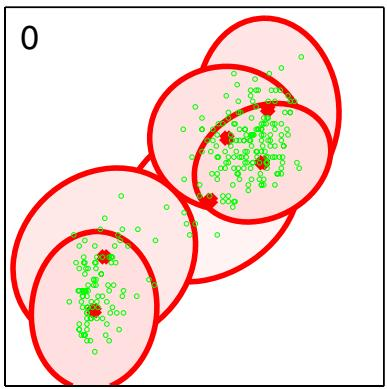
\includegraphics[keepaspectratio,alt={image}]{images/7d72e89259b6c9e6214b5f7be8e406778690e71b6f8fd203a1070b80f0661ca8.jpg}}

\pandocbounded{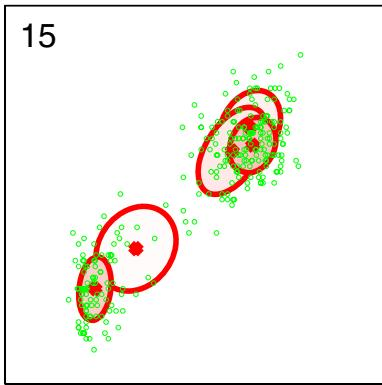
\includegraphics[keepaspectratio,alt={image}]{images/61dde09f523d50d5cee77d4317698f675d728703a4d85a978b6a8c9e8d2d8808.jpg}}

\pandocbounded{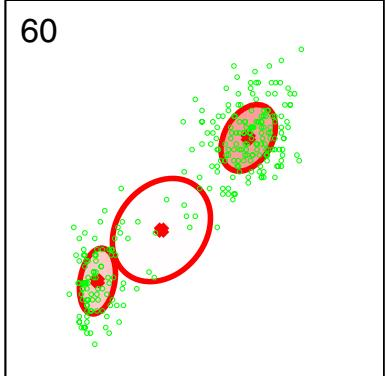
\includegraphics[keepaspectratio,alt={image}]{images/b8f24677a6cdda05165df3f4d63f204f3c1654869c76e2690f151cb4a4deffbe.jpg}}

\pandocbounded{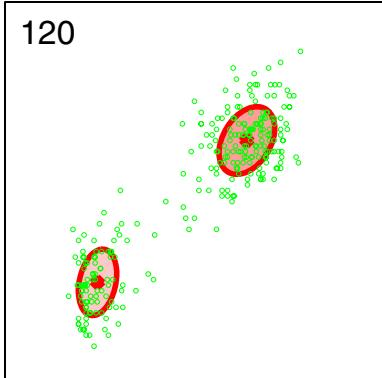
\includegraphics[keepaspectratio,alt={image}]{images/8960848dd2b03d633ed162c873aca51adaef8fceffe9deb4c58f4667e2a4ccba.jpg}}

the prior tightly constrains the mixing coefficients so that
\(\alpha _ { 0 }  \infty ,\) , then
\(\mathbb { E } [ \pi _ { k } ] \to\) \(1 / K\)

In Figure 10.6, the prior over the mixing coefficients is a Dirichlet of
the form (10.39). Recall from Figure 2.5 that for \(\alpha _ { 0 } < 1\)
the prior favours solutions in which some of the mixing coefficients are
zero. Figure 10.6 was obtained using \(\alpha _ { 0 } = 1 0 ^ { - 3 }\)
and resulted in two components having nonzero mixing coefficients. If
instead we choose \(\alpha _ { 0 } = 1\) we obtain three components with
nonzero mixing coefficients, and for \(\alpha = 1 0\) all six components
have nonzero mixing coefficients.

As we have seen there is a close similarity between the variational
solution for the Bayesian mixture of Gaussians and the EM algorithm for
maximum likelihood. In fact if we consider the limit \(N \to \infty\)
then the Bayesian treatment converges to the maximum likelihood EM
algorithm. For anything other than very small data sets, the dominant
computational cost of the variational algorithm for Gaussian mixtures
arises from the evaluation of the responsibilities, together with the
evaluation and inversion of the weighted data covariance matrices. These
computations mirror precisely those that arise in the maximum likelihood
EM algorithm, and so there is little computational overhead in using
this Bayesian approach as compared to the traditional maximum likelihood
one. There are, however, some substantial advantages. First of all, the
singularities that arise in maximum likelihood when a Gaussian component
`collapses' onto a specific data point are absent in the Bayesian
treatment.

Section 10.2.4

Indeed, these singularities are removed if we simply introduce a prior
and then use a MAP estimate instead of maximum likelihood. Furthermore,
there is no over-fitting if we choose a large number K of components in
the mixture, as we saw in Figure 10.6. Finally, the variational
treatment opens up the possibility of determining the optimal number of
components in the mixture without resorting to techniques such as cross
validation.

\subsection{10.2.2 Variational lower
bound}\label{variational-lower-bound}

We can also straightforwardly evaluate the lower bound (10.3) for this
model. In practice, it is useful to be able to monitor the bound during
the re-estimation in order to test for convergence. It can also provide
a valuable check on both the mathematical expressions for the solutions
and their software implementation, because at each step of the iterative
re-estimation procedure the value of this bound should not decrease. We
can take this a stage further to provide a deeper test of the
correctness of both the mathematical derivation of the update equations
and of their software implementation by using finite differences to
check that each update does indeed give a (constrained) maximum of the
bound (Svensen and Bishop, 2004). ´

For the variational mixture of Gaussians, the lower bound (10.3) is
given by

\[
\begin{array}{r c l} \mathcal {L} & = & \sum_ {\mathbf {Z}} \iiint q (\mathbf {Z}, \boldsymbol {\pi}, \boldsymbol {\mu}, \boldsymbol {\Lambda}) \ln \left\{\frac {p (\mathbf {X} , \mathbf {Z} , \boldsymbol {\pi} , \boldsymbol {\mu} , \boldsymbol {\Lambda})}{q (\mathbf {Z} , \boldsymbol {\pi} , \boldsymbol {\mu} , \boldsymbol {\Lambda})} \right\} \mathrm{d} \boldsymbol {\pi} \mathrm{d} \boldsymbol {\mu} \mathrm{d} \boldsymbol {\Lambda} \\ & = & \mathbb {E} [ \ln p (\mathbf {X}, \mathbf {Z}, \boldsymbol {\pi}, \boldsymbol {\mu}, \boldsymbol {\Lambda}) ] - \mathbb {E} [ \ln q (\mathbf {Z}, \boldsymbol {\pi}, \boldsymbol {\mu}, \boldsymbol {\Lambda}) ] \\ & = & \mathbb {E} [ \ln p (\mathbf {X} | \mathbf {Z}, \boldsymbol {\mu}, \boldsymbol {\Lambda}) ] + \mathbb {E} [ \ln p (\mathbf {Z} | \boldsymbol {\pi}) ] + \mathbb {E} [ \ln p (\boldsymbol {\pi}) ] + \mathbb {E} [ \ln p (\boldsymbol {\mu}, \boldsymbol {\Lambda}) ] \\ & & - \mathbb {E} [ \ln q (\mathbf {Z}) ] - \mathbb {E} [ \ln q (\boldsymbol {\pi}) ] - \mathbb {E} [ \ln q (\boldsymbol {\mu}, \boldsymbol {\Lambda}) ] \end{array} \tag {10}\tag{10.70}
\]

where, to keep the notation uncluttered, we have omitted the 
superscript on the \(q\) distributions, along with the subscripts on the
expectation operators because each expectation is taken with respect to
all of the random variables in its argument. The various terms in the
bound are easily evaluated to give the following results

\[
\begin{array}{c} \mathbb {E} [ \ln p (\mathbf {X} | \mathbf {Z}, \boldsymbol {\mu}, \boldsymbol {\Lambda}) ] = \frac {1}{2} \sum_ {k = 1} ^ {K} N _ {k} \left\{\ln \widetilde {\Lambda} _ {k} - D \beta_ {k} ^ {- 1} - \nu_ {k} \mathrm{Tr} (\mathbf {S} _ {k} \mathbf {W} _ {k}) \right. \\ \left. - \nu_ {k} (\overline {{\mathbf {x}}} _ {k} - \mathbf {m} _ {k}) ^ {\mathrm{T}} \mathbf {W} _ {k} (\overline {{\mathbf {x}}} _ {k} - \mathbf {m} _ {k}) - D \ln (2 \pi) \right\} \end{array}\tag{10.71}
\]

\[
\mathbb {E} [ \ln p (\mathbf {Z} | \boldsymbol {\pi}) ] = \sum_ {n = 1} ^ {N} \sum_ {k = 1} ^ {K} r _ {n k} \ln \widetilde {\pi} _ {k}\tag{10.72}
\]

\[
\mathbb {E} [ \ln p (\boldsymbol {\pi}) ] = \ln C (\boldsymbol {\alpha} _ {0}) + (\alpha_ {0} - 1) \sum_ {k = 1} ^ {K} \ln \widetilde {\pi} _ {k}\tag{10.73}
\]

\[
\begin{array}{l} \mathbb {E} [ \ln p (\boldsymbol {\mu}, \boldsymbol {\Lambda}) ] = \frac {1}{2} \sum_ {k = 1} ^ {K} \Bigg \{D \ln (\beta_ {0} / 2 \pi) + \ln \widetilde {\Lambda} _ {k} - \frac {D \beta_ {0}}{\beta_ {k}} \\ \qquad - \beta_ {0} \nu_ {k} (\mathbf {m} _ {k} - \mathbf {m} _ {0}) ^ {\mathrm{T}} \mathbf {W} _ {k} (\mathbf {m} _ {k} - \mathbf {m} _ {0}) \Bigg \} + K \ln B (\mathbf {W} _ {0}, \nu_ {0}) \\ \qquad + \frac {(\nu_ {0} - D - 1)}{2} \sum_ {k = 1} ^ {K} \ln \widetilde {\Lambda} _ {k} - \frac {1}{2} \sum_ {k = 1} ^ {K} \nu_ {k} \operatorname{Tr} (\mathbf {W} _ {0} ^ {- 1} \mathbf {W} _ {k}) \end{array}\tag{10.74}
\]

\[
\mathbb {E} [ \ln q (\mathbf {Z}) ] = \sum_ {n = 1} ^ {N} \sum_ {k = 1} ^ {K} r _ {n k} \ln r _ {n k}\tag{10.75}
\]

\[
\mathbb {E} [ \ln q (\boldsymbol {\pi}) ] = \sum_ {k = 1} ^ {K} \left(\alpha_ {k} - 1\right) \ln \widetilde {\pi} _ {k} + \ln C (\boldsymbol {\alpha})\tag{10.76}
\]

\[
\mathbb {E} [ \ln q (\pmb {\mu}, \pmb {\Lambda}) ] = \sum_ {k = 1} ^ {K} \left\{\frac {1}{2} \ln \widetilde {\Lambda} _ {k} + \frac {D}{2} \ln \left(\frac {\beta_ {k}}{2 \pi}\right) - \frac {D}{2} - \mathrm{H} [ q (\pmb {\Lambda} _ {k}) ] \right\}\tag{10.77}
\]

where \(D\) is the dimensionality of
\(\mathbf { x } , \mathrm { H } [ q ( \pmb { \Lambda } _ { k } ) ]\) is
the entropy of the Wishart distribution given by (B.82), and the
coefficients \(C ( \alpha )\) and \(B ( { \mathbf W } , \nu )\) are
defined by (B.23) and (B.79), respectively. Note that the terms
involving expectations of the logs of the \(q\) distributions simply
represent the negative entropies of those distributions. Some
simplifications and combination of terms can be performed when these
expressions are summed to give the lower bound. However, we have kept
the expressions separate for ease of understanding.

Finally, it is worth noting that the lower bound provides an alternative
approach for deriving the variational re-estimation equations obtained
in Section 10.2.1. To do this we use the fact that, since the model has
conjugate priors, the functional form of the factors in the variational
posterior distribution is known, namely discrete for \(\mathbf { Z } ,\)
Dirichlet for \(\pi ,\) , and Gaussian-Wishart for
\(( \mu _ { k } , \Lambda _ { k } )\) . By taking general parametric
forms for these distributions we can derive the form of the lower bound
as a function of the parameters of the distributions. Maximizing the
bound with respect to these parameters then gives the required
re-estimation equations.

\subsection{10.2.3 Predictive density}\label{predictive-density}

In applications of the Bayesian mixture of Gaussians model we will often
be interested in the predictive density for a new value
\(\widehat { \mathbf { x } }\) of the observed variable.
\({ \mathrm { A s } } -\) sociated with this observation will be a
corresponding latent variable \({ \widehat { \mathbf { z } } } ,\) and
the predictive density is then given by

\[
p (\widehat {\mathbf {x}} | \mathbf {X}) = \sum_ {\widehat {\mathbf {z}}} \iiint p (\widehat {\mathbf {x}} | \widehat {\mathbf {z}}, \boldsymbol {\mu}, \boldsymbol {\Lambda}) p (\widehat {\mathbf {z}} | \boldsymbol {\pi}) p (\boldsymbol {\pi}, \boldsymbol {\mu}, \boldsymbol {\Lambda} | \mathbf {X}) \mathrm{d} \boldsymbol {\pi} \mathrm{d} \boldsymbol {\mu} \mathrm{d} \boldsymbol {\Lambda}\tag{10.78}
\]

where \(p ( \pi , \mu , \mathbf { A } | \mathbf { X } )\) is the
(unknown) true posterior distribution of the parameters. Using (10.37)
and (10.38) we can first perform the summation over
\(\widehat { \mathbf { z } }\) to give

\[
p (\widehat {\mathbf {x}} | \mathbf {X}) = \sum_ {k = 1} ^ {K} \iiint \pi_ {k} \mathcal {N} \left(\widehat {\mathbf {x}} | \boldsymbol {\mu} _ {k}, \boldsymbol {\Lambda} _ {k} ^ {- 1}\right) p (\boldsymbol {\pi}, \boldsymbol {\mu}, \boldsymbol {\Lambda} | \mathbf {X}) d \boldsymbol {\pi} d \boldsymbol {\mu} d \boldsymbol {\Lambda}.\tag{10.79}
\]

Because the remaining integrations are intractable, we approximate the
predictive density by replacing the true posterior distribution
\(p ( \pi , \mu , \mathbf { \Delta } \mathbf { \Delta } \mathbf { \Delta } )\)
with its variational approximation
\(q ( \pi ) q ( \pmb { \mu } , \pmb { \Lambda } )\) to give

\[
p (\widehat {\mathbf {x}} | \mathbf {X}) = \sum_ {k = 1} ^ {K} \iiint \pi_ {k} \mathcal {N} \left(\widehat {\mathbf {x}} | \boldsymbol {\mu} _ {k}, \boldsymbol {\Lambda} _ {k} ^ {- 1}\right) q (\boldsymbol {\pi}) q (\boldsymbol {\mu} _ {k}, \boldsymbol {\Lambda} _ {k}) \mathrm{d} \boldsymbol {\pi} \mathrm{d} \boldsymbol {\mu} _ {k} \mathrm{d} \boldsymbol {\Lambda} _ {k}\tag{10.80}
\]

where we have made use of the factorization (10.55) and in each term we
have implicitly integrated out all variables
\(\{ \mu _ { j } , \pmb { \Lambda } _ { j } \}\) for \(j \neq k\) The
remaining integrations can now be evaluated analytically giving a
mixture of Student's t-distributions

\[
p (\widehat {\mathbf {x}} | \mathbf {X}) = \frac {1}{\widehat {\alpha}} \sum_ {k = 1} ^ {K} \alpha_ {k} \mathrm{St} (\widehat {\mathbf {x}} | \mathbf {m} _ {k}, \mathbf {L} _ {k}, \nu_ {k} + 1 - D)\tag{10.81}
\]

in which the \(k ^ { \mathrm { t h } }\) component has mean
\(\mathbf { m } _ { k }\) , and the precision is given by

\[
\mathbf {L} _ {k} = \frac {(\nu_ {k} + 1 - D) \beta_ {k}}{(1 + \beta_ {k})} \mathbf {W} _ {k}\tag{10.82}
\]

in which \(\nu _ { k }\) is given by (10.63). When the size N of the
data set is large the predictive distribution (10.81) reduces to a
mixture of Gaussians.

\subsection{10.2.4 Determining the number of
components}\label{determining-the-number-of-components}

We have seen that the variational lower bound can be used to determine a
posterior distribution over the number K of components in the mixture
model. There is, however, one subtlety that needs to be addressed. For
any given setting of the parameters in a Gaussian mixture model (except
for specific degenerate settings), there will exist other parameter
settings for which the density over the observed variables will be
identical. These parameter values differ only through a re-labelling of
the components. For instance, consider a mixture of two Gaussians and a
single observed variable x, in which the parameters have the values
\(\pi _ { 1 } = a , \pi _ { 2 } = b , \mu _ { 1 } = c .\)
\(\mu _ { 2 } = d , \sigma _ { 1 } = e , \sigma _ { 2 } = f\) . Then the
parameter values
\(\pi _ { 1 } = b , \pi _ { 2 } = a , \mu _ { 1 } = d .\)
\(\mu _ { 2 } = c , \sigma _ { 1 } = f , \sigma _ { 2 } = e .\) , in
which the two components have been exchanged, will by symmetry give rise
to the same value of \(p ( x )\) . If we have a mixture model comprising
K components, then each parameter setting will be a member of a family
of K! equivalent settings.

In the context of maximum likelihood, this redundancy is irrelevant
because the parameter optimization algorithm (for example EM) will,
depending on the initialization of the parameters, find one specific
solution, and the other equivalent solutions play no role. In a Bayesian
setting, however, we marginalize over all possible

Plot of the variational lower bound versus the number K of components in
the Gaussian mixture model, for the Old Faithful data, showing a
distinct peak at \(K =\) 2 components. For each value of \(K\) , the
model is trained from 100 different random starts, and the results shown
as \(" + "\) symbols plotted with small random horizontal perturbations
so that they can be distinguished. Note that some solutions find
suboptimal local maxima, but that this happens infrequently.

\pandocbounded{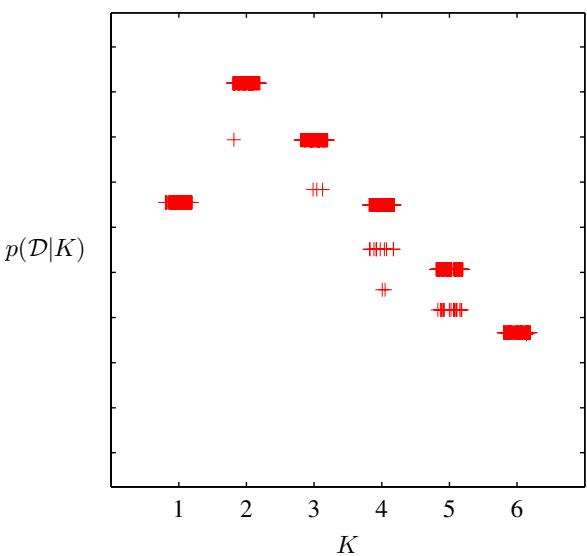
\includegraphics[keepaspectratio,alt={image}]{images/ea8189a03580e064e36d9035e4df2fbe6ae270e7a4ff175d5bb742f45ced6356.jpg}}

parameter values. We have seen in Figure 10.2 that if the true posterior
distribution is multimodal, variational inference based on the
minimization of KL \(( q \| p )\) will tend to approximate the
distribution in the neighbourhood of one of the modes and ignore the
others. Again, because equivalent modes have equivalent predictive
densities, this is of no concern provided we are considering a model
having a specific number K of components. If, however, we wish to
compare different values of K, then we need to take account of this
multimodality. A simple approximate solution is to add a term ln K! onto
the lower bound when used for model comparison and averaging.

Figure 10.7 shows a plot of the lower bound, including the multimodality
factor, versus the number K of components for the Old Faithful data set.
It is worth emphasizing once again that maximum likelihood would lead to
values of the likelihood function that increase monotonically with K
(assuming the singular solutions have been avoided, and discounting the
effects of local maxima) and so cannot be used to determine an
appropriate model complexity. By contrast, Bayesian inference
automatically makes the trade-off between model complexity and fitting
the data.

This approach to the determination of K requires that a range of models
having different K values be trained and compared. An alternative
approach to determining a suitable value for K is to treat the mixing
coefficients π as parameters and make point estimates of their values by
maximizing the lower bound (Corduneanu and Bishop, 2001) with respect to
\(\pi\) instead of maintaining a probability distribution over them as
in the fully Bayesian approach. This leads to the re-estimation equation

\[
\pi_ {k} = \frac {1}{N} \sum_ {n = 1} ^ {N} r _ {n k}\tag{10.83}
\]

and this maximization is interleaved with the variational updates for
the \(q\) distribution over the remaining parameters. Components that
provide insufficient contribution to explaining the data will have their
mixing coefficients driven to zero during the optimization, and so they
are effectively removed from the model through automatic relevance
determination. This allows us to make a single training run in which we
start with a relatively large initial value of K, and allow surplus
components to be pruned out of the model. The origins of the sparsity
when optimizing with respect to hyperparameters is discussed in detail
in the context of the relevance vector machine.

\subsection{10.2.5 Induced factorizations}\label{induced-factorizations}

In deriving these variational update equations for the Gaussian mixture
model, we assumed a particular factorization of the variational
posterior distribution given by (10.42). However, the optimal solutions
for the various factors exhibit additional factorizations. In
particular, the solution for
\(q ^ { \star } ( \pmb { \mu } , \pmb { \Lambda } )\) is given by the
product of an independent distribution
\(q ^ { \star } ( \pmb { \mu } _ { k } , \pmb { \Lambda } _ { k } )\)
over each of the components k of the mixture, whereas the variational
posterior distribution \(q ^ { \star } ( \mathbf { Z } )\) over the
latent variables, given by (10.48), factorizes into an independent
distribution \({ { q } ^ { \star } } ( { \bf { z } } _ { n } )\) for
each observation n (note that it does not further factorize with respect
to k because, for each value of \(n _ { \mathrm { : } }\) the
\(z _ { n k }\) are constrained to sum to one over k). These additional
factorizations are a consequence of the interaction between the assumed
factorization and the conditional independence properties of the true
distribution, as characterized by the directed graph in Figure 10.5.

We shall refer to these additional factorizations as induced
factorizations because they arise from an interaction between the
factorization assumed in the variational posterior distribution and the
conditional independence properties of the true joint distribution. In a
numerical implementation of the variational approach it is important to
take account of such additional factorizations. For instance, it would
be very inefficient to maintain a full precision matrix for the Gaussian
distribution over a set of variables if the optimal form for that
distribution always had a diagonal precision matrix (corresponding to a
factorization with respect to the individual variables described by that
Gaussian).

Such induced factorizations can easily be detected using a simple
graphical test based on d-separation as follows. We partition the latent
variables into three disjoint groups A, B, C and then let us suppose
that we are assuming a factorization between C and the remaining latent
variables, so that

\[
q (\mathbf {A}, \mathbf {B}, \mathbf {C}) = q (\mathbf {A}, \mathbf {B}) q (\mathbf {C}).\tag{10.84}
\]

Using the general result (10.9), together with the product rule for
probabilities, we see that the optimal solution for
\(q ( \mathbf { A } , \mathbf { B } )\) is given by

\[
\begin{array}{r c l} \ln q ^ {\star} (\mathbf {A}, \mathbf {B}) & = & \mathbb {E} _ {\mathbf {C}} [ \ln p (\mathbf {X}, \mathbf {A}, \mathbf {B}, \mathbf {C}) ] + \mathrm{const} \\ & = & \mathbb {E} _ {\mathbf {C}} [ \ln p (\mathbf {A}, \mathbf {B} | \mathbf {X}, \mathbf {C}) ] + \mathrm{const}. \end{array}\tag{10.85}
\]

We now ask whether this resulting solution will factorize between A and
B, in other words whether
\(q ^ { \star } ( { \bf A } , { \bf B } ) = q ^ { \star } ( { \bf A } ) q ^ { \star } ( { \bf B } )\)
. This will happen if, and only if, ln
\(p ( \mathbf { A } , \mathbf { B } | \mathbf { X } , \mathbf { C } ) = \ln p ( \mathbf { A } | \mathbf { X } , \mathbf { C } ) + \ln p ( \mathbf { B } | \mathbf { X } , \mathbf { C } )\)
, that is, if the conditional independence relation

\[
\mathbf {A} \perp \perp \mathbf {B} | \mathbf {X}, \mathbf {C}\tag{10.86}
\]

is satisfied. We can test to see if this relation does hold, for any
choice of A and B by making use of the d-separation criterion.

To illustrate this, consider again the Bayesian mixture of Gaussians
represented by the directed graph in Figure 10.5, in which we are
assuming a variational factorization given by (10.42). We can see
immediately that the variational posterior distribution over the
parameters must factorize between \(\pi\) and the remaining parameters
\(\pmb { \mu }\) and Λ because all paths connecting \(\pi\) to either
\(\pmb { \mu }\) or Λ must pass through one of the nodes
\(\mathbf { z } _ { n }\) all of which are in the conditioning set for
our conditional independence test and all of which are head-to-tail with
respect to such paths.

\subsection{10.3. Variational Linear
Regression}\label{variational-linear-regression}

As a second illustration of variational inference, we return to the
Bayesian linear regression model of Section 3.3. In the evidence
framework, we approximated the integration over \(\alpha\) and \(\beta\)
by making point estimates obtained by maximizing the log marginal
likelihood. A fully Bayesian approach would integrate over the
hyperparameters as well as over the parameters. Although exact
integration is intractable, we can use variational methods to find a
tractable approximation. In order to simplify the discussion, we shall
suppose that the noise precision parameter \(\beta\) is known, and is
fixed to its true value, although the framework is easily extended to
include the distribution over \(\beta .\) For the linear regression
model, the variational treatment will turn out to be equivalent to the
evidence framework. Nevertheless, it provides a good exercise in the use
of variational methods and will also lay the foundation for variational
treatment of Bayesian logistic regression in Section 10.6.

Recall that the likelihood function for w, and the prior over w, are
given by

\[
p (\mathbf {t} | \mathbf {w}) = \prod_ {n = 1} ^ {N} \mathcal {N} (t _ {n} | \mathbf {w} ^ {\mathrm{T}} \boldsymbol {\phi} _ {n}, \beta^ {- 1})\tag{10.87}
\]

\[
{p (\mathbf {w} | \alpha)} = {\mathcal {N} (\mathbf {w} | \mathbf {0}, \alpha^ {- 1} \mathbf {I})}\tag{10.88}
\]

where \(\phi _ { n } = \phi ( \mathbf { x } _ { n } )\) . We now
introduce a prior distribution over α. From our discussion in Section
2.3.6, we know that the conjugate prior for the precision of a Gaussian
is given by a gamma distribution, and so we choose

\[
p (\alpha) = \operatorname{Gam} (\alpha | a _ {0}, b _ {0})\tag{10.89}
\]

where \(\mathrm { G a m } ( \cdot | \cdot , \cdot )\) is defined by
(B.26). Thus the joint distribution of all the variables is given by

\[
p (\mathbf {t}, \mathbf {w}, \alpha) = p (\mathbf {t} | \mathbf {w}) p (\mathbf {w} | \alpha) p (\alpha).\tag{10.90}
\]

This can be represented as a directed graphical model as shown in Figure
10.8.

\subsection{10.3.1 Variational
distribution}\label{variational-distribution-1}

Our first goal is to find an approximation to the posterior distribution
\(p ( \mathbf { w } , \alpha \vert \mathbf { t } )\) To do this, we
employ the variational framework of Section 10.1, with a variational

Figure 10.8 Probabilistic graphical model representing the joint
distribution (10.90) for the Bayesian linear regression model.

\pandocbounded{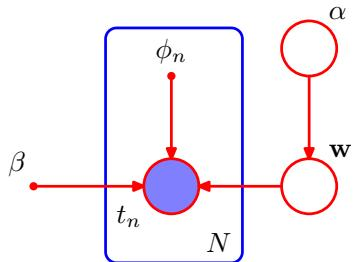
\includegraphics[keepaspectratio,alt={image}]{images/2ef586d449c7a500759983725786420c8745cfd31f0184c73314f0b62b4a3f97.jpg}}

posterior distribution given by the factorized expression

\[
q (\mathbf {w}, \alpha) = q (\mathbf {w}) q (\alpha).\tag{10.91}
\]

We can find re-estimation equations for the factors in this distribution
by making use of the general result (10.9). Recall that for each factor,
we take the log of the joint distribution over all variables and then
average with respect to those variables not in that factor. Consider
first the distribution over α. Keeping only terms that have a functional
dependence on α, we have

\[
\begin{array}{r l} & {\ln q ^ {\star} (\alpha) = \ln p (\alpha) + \mathbb {E} _ {\mathbf {w}} [ \ln p (\mathbf {w} | \alpha) ] + \mathrm{const}} \\ & {\quad = (a _ {0} - 1) \ln \alpha - b _ {0} \alpha + \frac {M}{2} \ln \alpha - \frac {\alpha}{2} \mathbb {E} [ \mathbf {w} ^ {\mathrm{T}} \mathbf {w} ] + \mathrm{const}.} \end{array}\tag{10.92}
\]

We recognize this as the log of a gamma distribution, and so identifying
the coefficients of α and ln α we obtain

\[
q ^ {\star} (\alpha) = \operatorname{Gam} (\alpha | a _ {N}, b _ {N})\tag{10.93}
\]

where

\[
a _ {N} = a _ {0} + \frac {M}{2}\tag{10.94}
\]

\[
{b _ {N}} = {b _ {0} + \frac {1}{2} \mathbb {E} [ \mathbf {w} ^ {\mathrm{T}} \mathbf {w} ].}\tag{10.95}
\]

Similarly, we can find the variational re-estimation equation for the
posterior distribution over w. Again, using the general result (10.9),
and keeping only those terms that have a functional dependence on w, we
have

\[
\ln q ^ {\star} (\mathbf {w}) = \ln p (\mathbf {t} | \mathbf {w}) + \mathbb {E} _ {\alpha} [ \ln p (\mathbf {w} | \alpha) ] + \mathrm{const}\tag{10.96}
\]

\[
{ = } { - \frac { \beta } { 2 } \sum _ { n = 1 } ^ { N } \{ \mathbf { w } ^ { \mathrm{T} } \boldsymbol { \phi } _ { n } - t _ { n } \} ^ { 2 } - \frac { 1 } { 2 } \mathbb { E } [ \alpha ] \mathbf { w } ^ { \mathrm{T} } \mathbf { w } + \mathrm{const} }\tag{10.97}
\]

\[
{ = } { - \frac { 1 } { 2 } \mathbf { w } ^ { \mathrm{T} } \left( \mathbb { E } [ \alpha ] \mathbf { I } + \beta \pmb { \Phi } ^ { \mathrm{T} } \pmb { \Phi } \right) \mathbf { w } + \beta \mathbf { w } ^ { \mathrm{T} } \pmb { \Phi } ^ { \mathrm{T} } \mathbf { t } + \mathrm{const.} }\tag{10.98}
\]

Because this is a quadratic form, the distribution
\(q ^ { \star } ( \mathbf { w } )\) is Gaussian, and so we can complete
the square in the usual way to identify the mean and covariance, giving

\[
q ^ {\star} (\mathbf {w}) = \mathcal {N} (\mathbf {w} | \mathbf {m} _ {N}, \mathbf {S} _ {N})\tag{10.99}
\]

where

\[
{\mathbf m} _ {N} = \beta {\mathbf S} _ {N} {\mathbf \Phi} ^ {\mathrm{T}} {\mathbf t}\tag{10.100}
\]

\[
\mathbf {S} _ {N} = \left(\mathbb {E} [ \alpha ] \mathbf {I} + \beta \boldsymbol {\Phi} ^ {\mathrm{T}} \boldsymbol {\Phi}\right) ^ {- 1}.\tag{10.101}
\]

Note the close similarity to the posterior distribution (3.52) obtained
when α was treated as a fixed parameter. The difference is that here α
is replaced by its expectation \(\mathbb { E } [ \alpha ]\) under the
variational distribution. Indeed, we have chosen to use the same
notation for the covariance matrix \(\mathbf { S } _ { N }\) in both
cases.

Using the standard results (B.27), (B.38), and (B.39), we can obtain the
required moments as follows

\[
\mathbb {E} [ \alpha ] = a _ {N} / b _ {N}\tag{10.102}
\]

\[
{\mathbb {E} [ \mathbf {w w} ^ {\mathrm{T}} ]} = {\mathbf {m} _ {N} \mathbf {m} _ {N} ^ {\mathrm{T}} + \mathbf {S} _ {N}.}\tag{10.103}
\]

The evaluation of the variational posterior distribution begins by
initializing the parameters of one of the distributions
\(q ( \mathbf { w } )\) or \(q ( \alpha )\) , and then alternately
re-estimates these factors in turn until a suitable convergence
criterion is satisfied (usually specified in terms of the lower bound to
be discussed shortly).

It is instructive to relate the variational solution to that found using
the evidence framework in Section 3.5. To do this consider the case
\(a _ { 0 } = b _ { 0 } = 0\) , corresponding to the limit of an
infinitely broad prior over α. The mean of the variational posterior
distribution \(q ( \alpha )\) is then given by

\[
\mathbb {E} [ \alpha ] = \frac {a _ {N}}{b _ {N}} = \frac {M / 2}{\mathbb {E} [ \mathbf {w} ^ {\mathrm{T}} \mathbf {w} ] / 2} = \frac {M}{\mathbf {m} _ {N} ^ {\mathrm{T}} \mathbf {m} _ {N} + \operatorname{Tr} (\mathbf {S} _ {N})}.\tag{10.104}
\]

Comparison with (9.63) shows that in the case of this particularly
simple model, the variational approach gives precisely the same
expression as that obtained by maximizing the evidence function using EM
except that the point estimate for α is replaced by its expected value.
Because the distribution \(q ( \mathbf { w } )\) depends on
\(q ( \alpha )\) only through the expectation
\(\mathbb { E } [ \alpha ]\) , we see that the two approaches will give
identical results for the case of an infinitely broad prior.

\subsection{10.3.2 Predictive
distribution}\label{predictive-distribution}

The predictive distribution over t, given a new input x, is easily
evaluated for this model using the Gaussian variational posterior for
the parameters

\[
\begin{array}{r c l} p (t | \mathbf {x}, \mathbf {t}) & = & \int p (t | \mathbf {x}, \mathbf {w}) p (\mathbf {w} | \mathbf {t})   \mathrm{d} \mathbf {w} \\ & \simeq & \int p (t | \mathbf {x}, \mathbf {w}) q (\mathbf {w})   \mathrm{d} \mathbf {w} \\ & = & \int \mathcal {N} (t | \mathbf {w} ^ {\mathrm{T}} \phi (\mathbf {x}), \beta^ {- 1}) \mathcal {N} (\mathbf {w} | \mathbf {m} _ {N}, \mathbf {S} _ {N})   \mathrm{d} \mathbf {w} \\ & = & \mathcal {N} (t | \mathbf {m} _ {N} ^ {\mathrm{T}} \phi (\mathbf {x}), \sigma^ {2} (\mathbf {x})) \end{array}\tag{10.105}
\]

where we have evaluated the integral by making use of the result (2.115)
for the linear-Gaussian model. Here the input-dependent variance is
given by

\[
\sigma^ {2} (\mathbf {x}) = \frac {1}{\beta} + \phi (\mathbf {x}) ^ {\mathrm{T}} \mathbf {S} _ {N} \phi (\mathbf {x}).\tag{10.106}
\]

Note that this takes the same form as the result (3.59) obtained with
fixed α except that now the expected value \(\mathbb { E } [ \alpha ]\)
appears in the definition of \(\mathbf { S } _ { N }\)

\subsection{10.3.3 Lower bound}\label{lower-bound}

Another quantity of importance is the lower bound defined by

\[
\begin{array}{r c l} \mathcal {L} (q) & = & \mathbb {E} [ \ln p (\mathbf {w}, \alpha , \mathbf {t}) ] - \mathbb {E} [ \ln q (\mathbf {w}, \alpha) ] \\ & = & \mathbb {E} _ {\mathbf {w}} [ \ln p (\mathbf {t} | \mathbf {w}) ] + \mathbb {E} _ {\mathbf {w}, \alpha} [ \ln p (\mathbf {w} | \alpha) ] + \mathbb {E} _ {\alpha} [ \ln p (\alpha) ] \\ & & - \mathbb {E} _ {\alpha} [ \ln q (\mathbf {w}) ] _ {\mathbf {w}} - \mathbb {E} [ \ln q (\alpha) ]. \end{array}\tag{10.107}
\]

Exercise 10.27

Evaluation of the various terms is straightforward, making use of
results obtained in previous chapters, and gives

\[
\begin{array}{r l r} \mathbb {E} [ \ln p (\mathbf {t} | \mathbf {w}) ] _ {\mathbf {w}} & = & \frac {N}{2} \ln \left(\frac {\beta}{2 \pi}\right) - \frac {\beta}{2} \mathbf {t} ^ {\mathrm{T}} \mathbf {t} + \beta \mathbf {m} _ {N} ^ {\mathrm{T}} \boldsymbol {\Phi} ^ {\mathrm{T}} \mathbf {t} \\ & & - \frac {\beta}{2} \mathrm{Tr} \left[ \boldsymbol {\Phi} ^ {\mathrm{T}} \boldsymbol {\Phi} (\mathbf {m} _ {N} \mathbf {m} _ {N} ^ {\mathrm{T}} + \mathbf {S} _ {N}) \right] \end{array}\tag{10.108}
\]

\[
\begin{array}{r c l} \mathbb {E} [ \ln p (\mathbf {w} | \alpha) ] _ {\mathbf {w}, \alpha} & = & - \frac {M}{2} \ln (2 \pi) + \frac {M}{2} (\psi (a _ {N}) - \ln b _ {N}) \\ & & - \frac {a _ {N}}{2 b _ {N}} \left[ \mathbf {m} _ {N} ^ {\mathrm{T}} \mathbf {m} _ {N} + \operatorname{Tr} (\mathbf {S} _ {N}) \right] \end{array}\tag{10.109}
\]

\[
\begin{array}{r c l} \mathbb {E} [ \ln p (\alpha) ] _ {\alpha} & = & a _ {0} \ln b _ {0} + (a _ {0} - 1) [ \psi (a _ {N}) - \ln b _ {N} ] \\ & & - b _ {0} \frac {a _ {N}}{b _ {N}} - \ln \Gamma (a _ {N}) \end{array}\tag{10.110}
\]

\[
{- \mathbb {E} [ \ln q (\mathbf {w}) ] _ {\mathbf {w}}} = {\frac {1}{2} \ln | \mathbf {S} _ {N} | + \frac {M}{2} [ 1 + \ln (2 \pi) ]}\tag{10.111}
\]

\[
- \mathbb {E} [ \ln q (\alpha) ] _ {\alpha} = \ln \Gamma (a _ {N}) - (a _ {N} - 1) \psi (a _ {N}) - \ln b _ {N} + a _ {N}.\tag{10.112}
\]

Figure 10.9 shows a plot of the lower bound \(\mathcal { L } ( q )\)
versus the degree of a polynomial model for a synthetic data set
generated from a degree three polynomial. Here the prior parameters have
been set to \(a _ { 0 } = b _ { 0 } = 0 .\) , corresponding to the
noninformative prior \(p ( \alpha ) \propto 1 / \alpha\) , which is
uniform over ln α as discussed in Section 2.3.6. As we saw in Section
10.1, the quantity \(\mathcal { L }\) represents lower bound on the log
marginal likelihood \(p ( \mathbf { t } | M )\) for the model. If we
assign equal prior probabilities \(p ( M )\) to the different values of
\(M .\) , then we can interpret \(\mathcal { L }\) as an approximation
to the posterior model probability \(p ( M | \mathbf { t } )\) . Thus
the variational framework assigns the highest probability to the model
with \(M = 3\) . This should be contrasted with the maximum likelihood
result, which assigns ever smaller residual error to models of
increasing complexity until the residual error is driven to zero,
causing maximum likelihood to favour severely over-fitted models.

Plot of the lower bound versus the order M of the polynomial, for a
polynomial model, in which a set of 10 data points is generated from a
polynomial with \(M \ = \ 3\) sampled over the interval ( 5, 5) with
additive Gaussian noise of variance 0.09. The value of the bound gives
the log probability of the model, and we see that the value of the bound
peaks at \(M = 3\) , corresponding to the true model from which the data
set was generated.

\pandocbounded{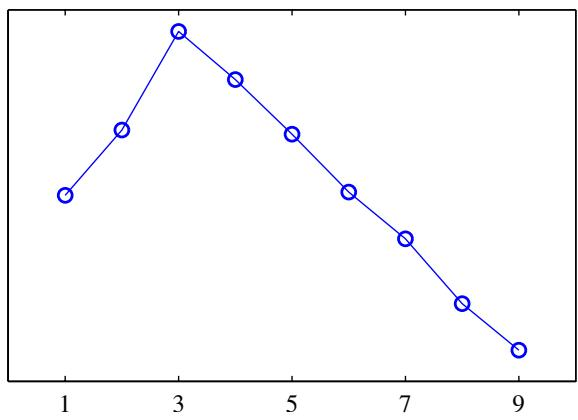
\includegraphics[keepaspectratio,alt={image}]{images/9ffeb658e891477f9ab40bdb0be977d105589663b26aa85206f178bff1cdd4c4.jpg}}

\subsection{10.4. Exponential Family
Distributions}\label{exponential-family-distributions}

In Chapter 2, we discussed the important role played by the exponential
family of distributions and their conjugate priors. For many of the
models discussed in this book, the complete-data likelihood is drawn
from the exponential family. However, in general this will not be the
case for the marginal likelihood function for the observed data. For
example, in a mixture of Gaussians, the joint distribution of
observations \({ \bf x } _ { n }\) and corresponding hidden variables
\(\mathbf { z } _ { n }\) is a member of the exponential family, whereas
the marginal distribution of \({ \bf x } _ { n }\) is a mixture of
Gaussians and hence is not.

Up to now we have grouped the variables in the model into observed
variables and hidden variables. We now make a further distinction
between latent variables, denoted Z, and parameters, denoted
\(\theta ,\) where parameters are intensive (fixed in number independent
of the size of the data set), whereas latent variables are extensive
(scale in number with the size of the data set). For example, in a
Gaussian mixture model, the indicator variables \(z _ { k n }\) (which
specify which component k is responsible for generating data point
\(\mathbf { x } _ { n } )\) represent the latent variables, whereas the
means \(\pmb { \mu } _ { k }\) precisions
\(\mathbf { \Lambda } _ { \Lambda _ { k } }\) and mixing proportions
\(\pi _ { k }\) represent the parameters.

Consider the case of independent identically distributed data. We denote
the data values by \({ \bf X } = \{ { \bf x } _ { n } \}\) , where
\(n = 1 , \ldots N\) , with corresponding latent variables
\({ \bf Z } = \{ { \bf z } _ { n } \}\) . Now suppose that the joint
distribution of observed and latent variables is a member of the
exponential family, parameterized by natural parameters η so that

\[
p (\mathbf {X}, \mathbf {Z} | \boldsymbol {\eta}) = \prod_ {n = 1} ^ {N} h (\mathbf {x} _ {n}, \mathbf {z} _ {n}) g (\boldsymbol {\eta}) \exp \left\{\boldsymbol {\eta} ^ {\mathrm{T}} \mathbf {u} (\mathbf {x} _ {n}, \mathbf {z} _ {n}) \right\}.\tag{10.113}
\]

We shall also use a conjugate prior for η, which can be written as

\[
p (\boldsymbol {\eta} | \nu_ {0}, \mathbf {v} _ {0}) = f (\nu_ {0}, \boldsymbol {\chi} _ {0}) g (\boldsymbol {\eta}) ^ {\nu_ {0}} \exp \left\{\nu_ {o} \boldsymbol {\eta} ^ {\mathrm{T}} \boldsymbol {\chi} _ {0} \right\}.\tag{10.114}
\]

Recall that the conjugate prior distribution can be interpreted as a
prior number \(\nu _ { 0 }\) of observations all having the value
\(x _ { 0 }\) for the u vector. Now consider a variational distribution
that factorizes between the latent variables and the parameters, so that
\(q ( { \bf Z } , \eta ) = q ( { \bf Z } ) q ( \eta )\) . Using the
general result (10.9), we can solve for the two factors as follows

\[
\begin{array}{r c l} \ln q ^ {\star} (\mathbf {Z}) & = & \mathbb {E} _ {\boldsymbol {\eta}} [ \ln p (\mathbf {X}, \mathbf {Z} | \boldsymbol {\eta}) ] + \text { const } \\ & = & \sum_ {n = 1} ^ {N} \left\{\ln h (\mathbf {x} _ {n}, \mathbf {z} _ {n}) + \mathbb {E} [ \boldsymbol {\eta} ^ {\mathrm{T}} ] \mathbf {u} (\mathbf {x} _ {n}, \mathbf {z} _ {n}) \right\} + \text { const }. \end{array}\tag{10.115}
\]

Thus we see that this decomposes into a sum of independent terms, one
for each value of \(n ,\) and hence the solution for
\(q ^ { \star } ( \mathbf { Z } )\) will factorize over \(n\) so that
\({ \boldsymbol { q } } ^ { \star } ( \mathbf { Z } ) =\)
\(\prod _ { n } q ^ { \star } ( \mathbf { z } _ { n } )\) . This is an
example of an induced factorization. Taking the exponential of both
sides, we have

\[
q ^ {\star} (\mathbf {z} _ {n}) = h (\mathbf {x} _ {n}, \mathbf {z} _ {n}) g \left(\mathbb {E} [ \boldsymbol {\eta} ]\right) \exp \left\{\mathbb {E} [ \boldsymbol {\eta} ^ {\mathrm{T}} ] \mathbf {u} (\mathbf {x} _ {n}, \mathbf {z} _ {n}) \right\}\tag{10.116}
\]

where the normalization coefficient has been re-instated by comparison
with the standard form for the exponential family.

Similarly, for the variational distribution over the parameters, we have

\[
\ln q ^ {\star} (\pmb {\eta}) = \ln p (\pmb {\eta} | \nu_ {0}, \pmb {\chi} _ {0}) + \mathbb {E} _ {\mathbf {Z}} [ \ln p (\mathbf {X}, \mathbf {Z} | \pmb {\eta}) ] + \mathrm{const}\tag{10.117}
\]

\[
= \nu_ {0} \ln g (\boldsymbol {\eta}) + \boldsymbol {\eta} ^ {\mathrm{T}} \boldsymbol {\chi} _ {0} + \sum_ {n = 1} ^ {N} \left\{\ln g (\boldsymbol {\eta}) + \boldsymbol {\eta} ^ {\mathrm{T}} \mathbb {E} _ {\mathbf {z} _ {n}} [ \mathbf {u} (\mathbf {x} _ {n}, \mathbf {z} _ {n}) ] \right\} + \text { const. }\tag{10.118}
\]

Again, taking the exponential of both sides, and re-instating the
normalization coefficient by inspection, we have

\[
q ^ {\star} (\boldsymbol {\eta}) = f \left(\nu_ {N}, \boldsymbol {\chi} _ {N}\right) g (\boldsymbol {\eta}) ^ {\nu_ {N}} \exp \left\{\boldsymbol {\eta} ^ {\mathrm{T}} \boldsymbol {\chi} _ {N} \right\}\tag{10.119}
\]

where we have defined

\[
\nu_ {N} = \nu_ {0} + N\tag{10.120}
\]

\[
\chi_ {N} = \chi_ {0} + \sum_ {n = 1} ^ {N} \mathbb {E} _ {\mathbf {z} _ {n}} [ \mathbf {u} (\mathbf {x} _ {n}, \mathbf {z} _ {n}) ].\tag{10.121}
\]

Note that the solutions for \(q ^ { \star } ( { \bf z } _ { n } )\) and
\(q ^ { \star } ( \eta )\) are coupled, and so we solve them iteratively
in a two-stage procedure. In the variational E step, we evaluate the
expected sufficient statistics
\(\mathbb { E } [ { \bf u } ( { \bf x } _ { n } , { \bf z } _ { n } ) ]\)
using the current posterior distribution \(q ( \mathbf { z } _ { n } )\)
over the latent variables and use this to compute a revised posterior
distribution \(q ( \eta )\) over the parameters. Then in the subsequent
variational M step, we use this revised parameter posterior distribution
to find the expected natural parameters
\(\mathbb { E } [ \eta ^ { \mathrm { T } } ]\) , which gives rise to a
revised variational distribution over the latent variables.

\subsection{10.4.1 Variational message
passing}\label{variational-message-passing}

We have illustrated the application of variational methods by
considering a specific model, the Bayesian mixture of Gaussians, in some
detail. This model can be described by the directed graph shown in
Figure 10.5. Here we consider more generally the use of variational
methods for models described by directed graphs and derive a number of
widely applicable results.

The joint distribution corresponding to a directed graph can be written
using the decomposition

\[
p (\mathbf {x}) = \prod_ {i} p (\mathbf {x} _ {i} | \mathrm{pa} _ {i})\tag{10.122}
\]

where \(\mathbf { x } _ { i }\) denotes the variable(s) associated with
node \(i ,\) and \(\mathrm { p a } _ { i }\) denotes the parent set
corresponding to node i. Note that \(\mathbf { x } _ { i }\) may be a
latent variable or it may belong to the set of observed variables. Now
consider a variational approximation in which the distribution
\(q ( \mathbf { x } )\) is assumed to factorize with respect to the
\(\mathbf { x } _ { i }\) so that

\[
q (\mathbf {x}) = \prod_ {i} q _ {i} (\mathbf {x} _ {i}).\tag{10.123}
\]

Note that for observed nodes, there is no factor
\(q ( \mathbf { x } _ { i } )\) in the variational distribution. We now
substitute (10.122) into our general result (10.9) to give

\[
\ln q _ {j} ^ {\star} (\mathbf {x} _ {j}) = \mathbb {E} _ {i \neq j} \left[ \sum_ {i} \ln p (\mathbf {x} _ {i} | \mathrm{pa} _ {i}) \right] + \text { const. }\tag{10.124}
\]

Any terms on the right-hand side that do not depend on
\(\mathbf { x } _ { j }\) can be absorbed into the additive constant. In
fact, the only terms that do depend on \(\mathbf { x } _ { j }\) are the
conditional distribution for \(\mathbf { x } _ { j }\) given by
\(p ( \mathbf { x } _ { j } | \mathrm { p a } _ { j } )\) together with
any other conditional distributions that have \(\mathbf { x } _ { j }\)
in the conditioning set. By definition, these conditional distributions
correspond to the children of node \(j\) , and they therefore also
depend on the co-parents of the child nodes, i.e., the other parents of
the child nodes besides node \(\mathbf { x } _ { j }\) itself. We see
that the set of all nodes on which
\(q ^ { \star } ( \mathbf { x } _ { j } )\) depends corresponds to the
Markov blanket of node \(\mathbf { x } _ { j }\) , as illustrated in
Figure 8.26. Thus the update of the factors in the variational posterior
distribution represents a local calculation on the graph. This makes
possible the construction of general purpose software for variational
inference in which the form of the model does not need to be specified
in advance (Bishop et al., 2003).

If we now specialize to the case of a model in which all of the
conditional distributions have a conjugate-exponential structure, then
the variational update procedure can be cast in terms of a local message
passing algorithm (Winn and Bishop, 2005). In particular, the
distribution associated with a particular node can be updated once that
node has received messages from all of its parents and all of its
children. This in turn requires that the children have already received
messages from their coparents. The evaluation of the lower bound can
also be simplified because many of the required quantities are already
evaluated as part of the message passing scheme. This distributed
message passing formulation has good scaling properties and is well
suited to large networks.

\subsection{10.5. Local Variational
Methods}\label{local-variational-methods}

The variational framework discussed in Sections 10.1 and 10.2 can be
considered a `global' method in the sense that it directly seeks an
approximation to the full posterior distribution over all random
variables. An alternative `local' approach involves finding bounds on
functions over individual variables or groups of variables within a
model. For instance, we might seek a bound on a conditional distribution
\(p ( y | x )\) which is itself just one factor in a much larger
probabilistic model specified by a directed graph. The purpose of
introducing the bound of course is to simplify the resulting
distribution. This local approximation can be applied to multiple
variables in turn until a tractable approximation is obtained, and in
Section 10.6.1 we shall give a practical example of this approach in the
context of logistic regression. Here we focus on developing the bounds
themselves.

We have already seen in our discussion of the Kullback-Leibler
divergence that the convexity of the logarithm function played a key
role in developing the lower bound in the global variational approach.
We have defined a (strictly) convex function as one for which every
chord lies above the function. Convexity also plays a central role in
the local variational framework. Note that our discussion will apply
equally to concave functions with `min' and `max' interchanged and with
lower bounds replaced by upper bounds.

Let us begin by considering a simple example, namely the function
\(f ( x ) =\) \(\exp ( - x )\) , which is a convex function of x, and
which is shown in the left-hand plot of Figure 10.10. Our goal is to
approximate \(f ( x )\) by a simpler function, in particular a linear
function of \(x .\) . From Figure 10.10, we see that this linear
function will be a lower bound on \(f ( x )\) if it corresponds to a
tangent. We can obtain the tangent line \(y ( x )\) at a specific value
of x, say \(x = \xi\) , by making a first order Taylor expansion

\[
y (x) = f (\xi) + f ^ {\prime} (\xi) (x - \xi)\tag{10.125}
\]

so that \(y ( x ) \leqslant f ( x )\) with equality when \(x = \xi\) .
For our example function \(f ( x ) =\)

Figure 10.10 In the left-hand figure the red curve shows the function
\(\exp ( - x )\) and the blue line shows the tangent at \(x \ = \ \xi\)
defined by (10.125) with \(\xi = 1\) . This line has slope
\(\overset { \cdot } { \lambda } = f ^ { \prime } ( \overset { \cdot } { \xi } ) = - \exp ( - \overset { \cdot } { \xi } )\)
. Note that any other tangent line, for example the ones shown in green,
will have a smaller value of \(y\) at \(x =\) \(\xi .\) The right-hand
figure shows the corresponding plot of the function
\(\lambda \xi - g ( \lambda )\) , where \(g ( \lambda )\) is given by
\(_ { ( 1 0 . 1 3 1 ) }\) versus λ for \(\xi ~ = ~ 1\) , in which the
maximum corresponds to \(\lambda = - \exp ( - \xi ) = - 1 / e\)

\pandocbounded{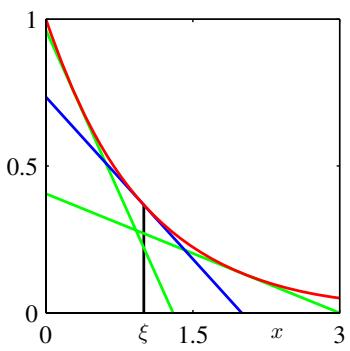
\includegraphics[keepaspectratio,alt={image}]{images/63e1e12514de1d28c720e8a02b7c8ecd571fb219b246bcbec34c83f0f59b7774.jpg}}

\pandocbounded{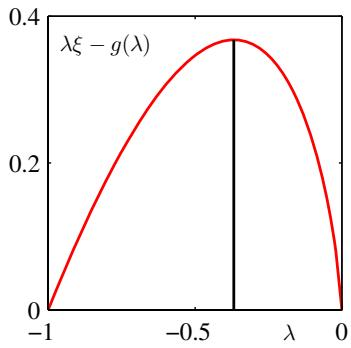
\includegraphics[keepaspectratio,alt={image}]{images/eafae9c5212bdd8f83a16e9d8202000be8607ed78cfafa4d163f36a469d84d79.jpg}}

\pandocbounded{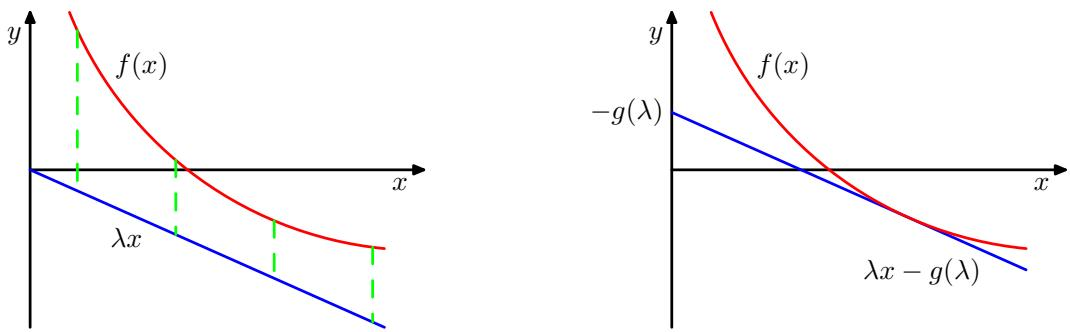
\includegraphics[keepaspectratio,alt={image}]{images/6c1cb78274e9abe116fe98cb2ecd3d6305933acc2a3fc160f4083d085a30603f.jpg}}

Figure 10.11 In the left-hand plot the red curve shows a convex function
\(f ( x )\) , and the blue line represents the linear function
\(\lambda x ,\) which is a lower bound on \(f ( x )\) because
\(f ( x ) > \lambda x\) for all x. For the given value of slope λ the
contact point of the tangent line having the same slope is found by
minimizing with respect to x the discrepancy (shown by the green dashed
lines) given by \(f ( x ) - \lambda x\) . This defines the dual function
\(g ( \lambda )\) , which corresponds to the (negative of the) intercept
of the tangent line having slope λ.

\(\exp ( - x )\) , we therefore obtain the tangent line in the form

\[
y (x) = \exp (- \xi) - \exp (- \xi) (x - \xi)\tag{10.126}
\]

which is a linear function parameterized by \(\xi .\) For consistency
with subsequent discussion, let us define \(\lambda = - \exp ( - \xi )\)
so that

\[
y (x, \lambda) = \lambda x - \lambda + \lambda \ln (- \lambda).\tag{10.127}
\]

Different values of λ correspond to different tangent lines, and because
all such lines are lower bounds on the function, we have
\(f ( x ) \geqslant y ( x , \lambda )\) . Thus we can write the function
in the form

\[
f (x) = \max _ {\lambda} \left\{\lambda x - \lambda + \lambda \ln (- \lambda) \right\}.\tag{10.128}
\]

We have succeeded in approximating the convex function \(f ( x )\) by a
simpler, linear function \(y ( x , \lambda )\) . The price we have paid
is that we have introduced a variational parameter λ, and to obtain the
tightest bound we must optimize with respect to λ.

We can formulate this approach more generally using the framework of
convex duality (Rockafellar, 1972; Jordan et al., 1999). Consider the
illustration of a convex function \(f ( x )\) shown in the left-hand
plot in Figure 10.11. In this example, the function λx is a lower bound
on \(f ( x )\) but it is not the best lower bound that can be achieved
by a linear function having slope λ, because the tightest bound is given
by the tangent line. Let us write the equation of the tangent line,
having slope λ as \(\lambda x - g ( \lambda )\) where the (negative)
intercept \(g ( \lambda )\) clearly depends on the slope λ of the
tangent. To determine the intercept, we note that the line must be moved
vertically by an amount equal to the smallest vertical distance between
the line and the function, as shown in Figure 10.11. Thus

\[
\begin{array}{r c l} g (\lambda) & = & - \min _ {x} \left\{f (x) - \lambda x \right\} \\ & = & \max _ {x} \left\{\lambda x - f (x) \right\}. \end{array}\tag{10.129}
\]

Now, instead of fixing λ and varying x, we can consider a particular x
and then adjust λ until the tangent plane is tangent at that particular
x. Because the y value of the tangent line at a particular x is
maximized when that value coincides with its contact point, we have

\[
f (x) = \max _ {\lambda} \left\{\lambda x - g (\lambda) \right\}.\tag{10.130}
\]

We see that the functions \(f ( x )\) and \(g ( \lambda )\) play a dual
role, and are related through (10.129) and (10.130).

Let us apply these duality relations to our simple example
\(f ( x ) = \exp ( - x )\) From (10.129) we see that the maximizing
value of x is given by \(\xi = - \ln ( - \lambda )\) , and
back-substituting we obtain the conjugate function \(g ( \lambda )\) in
the form

\[
g (\lambda) = \lambda - \lambda \ln (- \lambda)\tag{10.131}
\]

as obtained previously. The function \(\lambda \xi - g ( \lambda )\) is
shown, for \(\xi = 1\) in the right-hand plot in Figure 10.10. As a
check, we can substitute (10.131) into (10.130), which gives the
maximizing value of \(\lambda = - \exp ( - x )\) , and back-substituting
then recovers the original function \(f ( x ) = \exp ( - x )\)

For concave functions, we can follow a similar argument to obtain upper
bounds, in which max' is replaced with `min', so that

\[
f (x) = \min _ {\lambda} \{\lambda x - g (\lambda) \}\tag{10.132}
\]

\[
g (\lambda) = \min _ {x} \left\{\lambda x - f (x) \right\}.\tag{10.133}
\]

If the function of interest is not convex (or concave), then we cannot
directly apply the method above to obtain a bound. However, we can first
seek invertible transformations either of the function or of its
argument which change it into a convex form. We then calculate the
conjugate function and then transform back to the original variables.

An important example, which arises frequently in pattern recognition, is
the logistic sigmoid function defined by

\[
\sigma (x) = \frac {1}{1 + e ^ {- x}}.\tag{10.134}
\]

As it stands this function is neither convex nor concave. However, if we
take the logarithm we obtain a function which is concave, as is easily
verified by finding the second derivative. From (10.133) the
corresponding conjugate function then takes the form

\[
g (\lambda) = \min _ {x} \left\{\lambda x - f (x) \right\} = - \lambda \ln \lambda - (1 - \lambda) \ln (1 - \lambda)\tag{10.135}
\]

which we recognize as the binary entropy function for a variable whose
probability of having the value 1 is λ. Using (10.132), we then obtain
an upper bound on the log sigmoid

\[
\ln \sigma (x) \leqslant \lambda x - g (\lambda)\tag{10.136}
\]

\pandocbounded{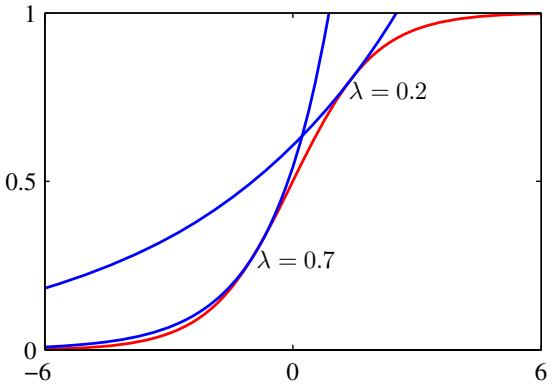
\includegraphics[keepaspectratio,alt={image}]{images/416ac1db4eff31ce3d429966080b12a7d4d20673717341f2d09826f58196cc61.jpg}}

\pandocbounded{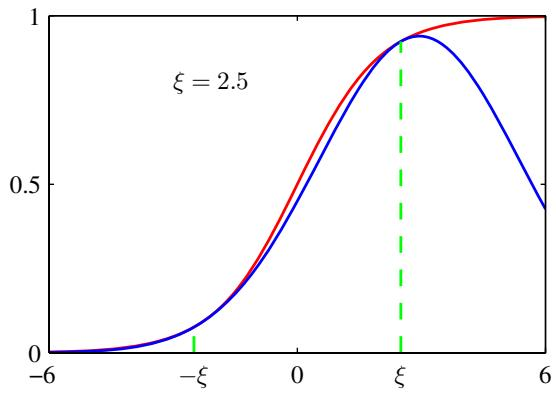
\includegraphics[keepaspectratio,alt={image}]{images/78cbdd76dd23597d2b41659982d8a2cf636b1a23d382d192f8a74505a0e5a225.jpg}}

Figure 10.12 The left-hand plot shows the logistic sigmoid function
\(\sigma ( x )\) defined by (10.134) in red, together with two examples
of the exponential upper bound (10.137) shown in blue. The right-hand
plot shows the logistic sigmoid again in red together with the Gaussian
lower bound (10.144) shown in blue. Here the parameter \(\xi = 2 . 5\) ,
and the bound is exact at \(x = \xi\) and \(x = - \xi\) , denoted by the
dashed green lines.

and taking the exponential, we obtain an upper bound on the logistic
sigmoid itself of the form

\[
\sigma (x) \leqslant \exp (\lambda x - g (\lambda))\tag{10.137}
\]

which is plotted for two values of λ on the left-hand plot in Figure
10.12.

We can also obtain a lower bound on the sigmoid having the functional
form of a Gaussian. To do this, we follow Jaakkola and Jordan (2000) and
make transformations both of the input variable and of the function
itself. First we take the log of the logistic function and then
decompose it so that

\[
\begin{array}{r c l} \ln \sigma (x) & = & - \ln (1 + e ^ {- x}) = - \ln \left\{e ^ {- x / 2} (e ^ {x / 2} + e ^ {- x / 2}) \right\} \\ & = & x / 2 - \ln (e ^ {x / 2} + e ^ {- x / 2}). \end{array}\tag{10.138}
\]

We now note that the function
\(f ( x ) = - \ln ( e ^ { x / 2 } + e ^ { - x / 2 } )\) is a convex
function of the variable \(x ^ { 2 }\) , as can again be verified by
finding the second derivative. This leads to a lower bound on
\(f ( x )\) , which is a linear function of \(x ^ { 2 }\) whose
conjugate function is given by

\[
g (\lambda) = \max _ {x ^ {2}} \left\{\lambda x ^ {2} - f \left(\sqrt {x ^ {2}}\right) \right\}.\tag{10.139}
\]

The stationarity condition leads to

\[
0 = \lambda - \frac {d x}{d x ^ {2}} \frac {d}{d x} f (x) = \lambda + \frac {1}{4 x} \tanh \left(\frac {x}{2}\right).\tag{10.140}
\]

If we denote this value of \(x ,\) corresponding to the contact point of
the tangent line for this particular value of λ, by \(\xi ,\) , then we
have

\[
\lambda (\xi) = - \frac {1}{4 \xi} \tanh \left(\frac {\xi}{2}\right) = - \frac {1}{2 \xi} \left[ \sigma (\xi) - \frac {1}{2} \right].\tag{10.141}
\]

Instead of thinking of \(\lambda\) as the variational parameter, we can
let \(\xi\) play this role as this leads to simpler expressions for the
conjugate function, which is then given by

\[
g (\lambda) = \lambda (\xi) \xi^ {2} - f (\xi) = \lambda (\xi) \xi^ {2} + \ln (e ^ {\xi / 2} + e ^ {- \xi / 2}).\tag{10.142}
\]

Hence the bound on \(f ( x )\) can be written as

\[
f (x) \geqslant \lambda x ^ {2} - g (\lambda) = \lambda x ^ {2} - \lambda \xi^ {2} - \ln (e ^ {\xi / 2} + e ^ {- \xi / 2}).\tag{10.143}
\]

The bound on the sigmoid then becomes

\[
\sigma (x) \geqslant \sigma (\xi) \exp \left\{(x - \xi) / 2 - \lambda (\xi) (x ^ {2} - \xi^ {2}) \right\}\tag{10.144}
\]

where \(\lambda ( \xi )\) is defined by (10.141). This bound is
illustrated in the right-hand plot of Figure 10.12. We see that the
bound has the form of the exponential of a quadratic function of \(x ,\)
which will prove useful when we seek Gaussian representations of
posterior distributions defined through logistic sigmoid functions.

The logistic sigmoid arises frequently in probabilistic models over
binary variables because it is the function that transforms a log odds
ratio into a posterior probability. The corresponding transformation for
a multiclass distribution is given by the softmax function.
Unfortunately, the lower bound derived here for the logistic sigmoid
does not directly extend to the softmax. Gibbs (1997) proposes a method
for constructing a Gaussian distribution that is conjectured to be a
bound (although no rigorous proof is given), which may be used to apply
local variational methods to multiclass problems.

We shall see an example of the use of local variational bounds in
Sections 10.6.1. For the moment, however, it is instructive to consider
in general terms how these bounds can be used. Suppose we wish to
evaluate an integral of the form

\[
I = \int \sigma (a) p (a) \mathrm{d} a\tag{10.145}
\]

where \(\sigma ( a )\) is the logistic sigmoid, and \(p ( a )\) is a
Gaussian probability density. Such integrals arise in Bayesian models
when, for instance, we wish to evaluate the predictive distribution, in
which case \(p ( a )\) represents a posterior parameter distribution.
Because the integral is intractable, we employ the variational bound
(10.144), which we write in the form
\(\sigma ( a ) \geqslant f ( a , \xi )\) where \(\xi\) is a variational
parameter. The integral now becomes the product of two
exponential-quadratic functions and so can be integrated analytically to
give a bound on I

\[
I \geqslant \int f (a, \xi) p (a) \mathrm{d} a = F (\xi).\tag{10.146}
\]

We now have the freedom to choose the variational parameter \(\xi ,\) ,
which we do by finding the value \(\xi ^ { \star }\) that maximizes the
function \(F ( \xi )\) . The resulting value \(F ( \xi ^ { \star } )\)
represents the tightest bound within this family of bounds and can be
used as an approximation to I. This optimized bound, however, will in
general not be exact.

Although the bound \(\sigma ( a ) \geqslant f ( a , \xi )\) on the
logistic sigmoid can be optimized exactly, the required choice for
\(\xi\) depends on the value of a, so that the bound is exact for one
value of a only. Because the quantity \(F ( \xi )\) is obtained by
integrating over all values of \(a ,\) the value of \(\xi ^ { \star }\)
represents a compromise, weighted by the distribution \(p ( a )\)

\subsection{10.6. Variational Logistic
Regression}\label{variational-logistic-regression}

We now illustrate the use of local variational methods by returning to
the Bayesian logistic regression model studied in Section 4.5. There we
focussed on the use of the Laplace approximation, while here we consider
a variational treatment based on the approach of Jaakkola and Jordan
(2000). Like the Laplace method, this also leads to a Gaussian
approximation to the posterior distribution. However, the greater
flexibility of the variational approximation leads to improved accuracy
compared to the Laplace method. Furthermore (unlike the Laplace method),
the variational approach is optimizing a well defined objective function
given by a rigourous bound on the model evidence. Logistic regression
has also been treated by Dybowski and Roberts (2005) from a Bayesian
perspective using Monte Carlo sampling techniques.

\subsection{10.6.1 Variational posterior
distribution}\label{variational-posterior-distribution}

Here we shall make use of a variational approximation based on the local
bounds introduced in Section 10.5. This allows the likelihood function
for logistic regression, which is governed by the logistic sigmoid, to
be approximated by the exponential of a quadratic form. It is therefore
again convenient to choose a conjugate Gaussian prior of the form
(4.140). For the moment, we shall treat the hyperparameters
\(\mathbf { m } _ { 0 }\) and \(\mathbf { S } _ { 0 }\) as fixed
constants. In Section 10.6.3, we shall demonstrate how the variational
formalism can be extended to the case where there are unknown
hyperparameters whose values are to be inferred from the data.

In the variational framework, we seek to maximize a lower bound on the
marginal likelihood. For the Bayesian logistic regression model, the
marginal likelihood takes the form

\[
p (\mathbf {t}) = \int p (\mathbf {t} | \mathbf {w}) p (\mathbf {w}) \mathrm{d} \mathbf {w} = \int \left[ \prod_ {n = 1} ^ {N} p (t _ {n} | \mathbf {w}) \right] p (\mathbf {w}) \mathrm{d} \mathbf {w}.\tag{10.147}
\]

We first note that the conditional distribution for t can be written as

\[
\begin{array}{r c l} p (t | \mathbf {w}) & = & \sigma (a) ^ {t} \left\{1 - \sigma (a) \right\} ^ {1 - t} \\ & = & \left(\frac {1}{1 + e ^ {- a}}\right) ^ {t} \left(1 - \frac {1}{1 + e ^ {- a}}\right) ^ {1 - t} \\ & = & e ^ {a t} \frac {e ^ {- a}}{1 + e ^ {- a}} = e ^ {a t} \sigma (- a) \end{array}\tag{10.148}
\]

where \(a = \mathbf { w } ^ { \mathrm { T } } \phi\) . In order to
obtain a lower bound on \(p ( \mathfrak { t } )\) , we make use of the
variational lower bound on the logistic sigmoid function given by
(10.144), which

we reproduce here for convenience

\[
\sigma (z) \geqslant \sigma (\xi) \exp \left\{(z - \xi) / 2 - \lambda (\xi) (z ^ {2} - \xi^ {2}) \right\}\tag{10.149}
\]

where

\[
\lambda (\xi) = \frac {1}{2 \xi} \left[ \sigma (\xi) - \frac {1}{2} \right].\tag{10.150}
\]

We can therefore write

\[
p (t | \mathbf {w}) = e ^ {a t} \sigma (- a) \geqslant e ^ {a t} \sigma (\xi) \exp \left\{- (a + \xi) / 2 - \lambda (\xi) (a ^ {2} - \xi^ {2}) \right\}.\tag{10.151}
\]

Note that because this bound is applied to each of the terms in the
likelihood function separately, there is a variational parameter
\(\xi _ { n }\) corresponding to each training set observation
\(( \phi _ { n } , t _ { n } )\) . Using
\(a = \mathbf { w } ^ { \mathrm { T } } \phi\) , and multiplying by the
prior distribution, we obtain the following bound on the joint
distribution of t and w

\[
p (\mathbf {t}, \mathbf {w}) = p (\mathbf {t} | \mathbf {w}) p (\mathbf {w}) \geqslant h (\mathbf {w}, \boldsymbol {\xi}) p (\mathbf {w})\tag{10.152}
\]

where \(\boldsymbol { \xi }\) denotes the set \(\{ \xi _ { n } \}\) of
variational parameters, and

\[
\begin{array}{r c l} h (\mathbf {w}, \boldsymbol {\xi}) & = & \prod_ {n = 1} ^ {N} \sigma (\xi_ {n}) \exp \left\{\mathbf {w} ^ {\mathrm{T}} \phi_ {n} t _ {n} - (\mathbf {w} ^ {\mathrm{T}} \phi_ {n} + \xi_ {n}) / 2 \right. \\ & & \left. - \lambda (\xi_ {n}) ([ \mathbf {w} ^ {\mathrm{T}} \phi_ {n} ] ^ {2} - \xi_ {n} ^ {2}) \right\}. \end{array}\tag{10.153}
\]

Evaluation of the exact posterior distribution would require
normalization of the lefthand side of this inequality. Because this is
intractable, we work instead with the right-hand side. Note that the
function on the right-hand side cannot be interpreted as a probability
density because it is not normalized. Once it is normalized to give a
variational posterior distribution \(q ( \mathbf { w } )\) , however, it
no longer represents a bound.

Because the logarithm function is monotonically increasing, the
inequality \(A \geqslant\) \(B\) implies ln \(A \geqslant\) ln \(B .\) .
This gives a lower bound on the log of the joint distribution of t and w
of the form

\[
\begin{array}{c} \ln \left\{p (\mathbf {t} | \mathbf {w}) p (\mathbf {w}) \right\} \geqslant \ln p (\mathbf {w}) + \sum_ {n = 1} ^ {N} \left\{\ln \sigma (\xi_ {n}) + \mathbf {w} ^ {\mathrm{T}} \phi_ {n} t _ {n} \right. \\ \left. - (\mathbf {w} ^ {\mathrm{T}} \phi_ {n} + \xi_ {n}) / 2 - \lambda (\xi_ {n}) ([ \mathbf {w} ^ {\mathrm{T}} \phi_ {n} ] ^ {2} - \xi_ {n} ^ {2}) \right\}. \end{array}\tag{10.154}
\]

Substituting for the prior \(p ( \mathbf { w } )\) , the right-hand side
of this inequality becomes, as a function of w

\[
\begin{array}{c} {- \frac {1}{2} (\mathbf {w} - \mathbf {m} _ {0}) ^ {\mathrm{T}} \mathbf {S} _ {0} ^ {- 1} (\mathbf {w} - \mathbf {m} _ {0})} \\ {+ \sum_ {n = 1} ^ {N} \left\{\mathbf {w} ^ {\mathrm{T}} \boldsymbol {\phi} _ {n} (t _ {n} - 1 / 2) - \lambda (\xi_ {n}) \mathbf {w} ^ {\mathrm{T}} (\boldsymbol {\phi} _ {n} \boldsymbol {\phi} _ {n} ^ {\mathrm{T}}) \mathbf {w} \right\} + \mathrm{const}.} \end{array}\tag{10.155}
\]

This is a quadratic function of w, and so we can obtain the
corresponding variational approximation to the posterior distribution by
identifying the linear and quadratic terms in w, giving a Gaussian
variational posterior of the form

\[
q (\mathbf {w}) = \mathcal {N} (\mathbf {w} | \mathbf {m} _ {N}, \mathbf {S} _ {N})\tag{10.156}
\]

where

\[
\mathbf {m} _ {N} = \mathbf {S} _ {N} \left(\mathbf {S} _ {0} ^ {- 1} \mathbf {m} _ {0} + \sum_ {n = 1} ^ {N} (t _ {n} - 1 / 2) \phi_ {n}\right)\tag{10.157}
\]

\[
\mathbf {S} _ {N} ^ {- 1} = \mathbf {S} _ {0} ^ {- 1} + 2 \sum_ {n = 1} ^ {N} \lambda (\xi_ {n}) \phi_ {n} \phi_ {n} ^ {\mathrm{T}}.\tag{10.158}
\]

As with the Laplace framework, we have again obtained a Gaussian
approximation to the posterior distribution. However, the additional
flexibility provided by the variational parameters \(\{ \xi _ { n } \}\)
leads to improved accuracy in the approximation (Jaakkola and Jordan,
2000).

Here we have considered a batch learning context in which all of the
training data is available at once. However, Bayesian methods are
intrinsically well suited to sequential learning in which the data
points are processed one at a time and then discarded. The formulation
of this variational approach for the sequential case is straightforward.

Note that the bound given by (10.149) applies only to the two-class
problem and so this approach does not directly generalize to
classification problems with \(K > 2\) classes. An alternative bound for
the multiclass case has been explored by Gibbs (1997).

\subsection{10.6.2 Optimizing the variational
parameters}\label{optimizing-the-variational-parameters}

We now have a normalized Gaussian approximation to the posterior
distribution, which we shall use shortly to evaluate the predictive
distribution for new data points. First, however, we need to determine
the variational parameters \(\{ \xi _ { n } \}\) by maximizing the lower
bound on the marginal likelihood.

To do this, we substitute the inequality (10.152) back into the marginal
likelihood to give

\[
\ln p (\mathbf {t}) = \ln \int p (\mathbf {t} | \mathbf {w}) p (\mathbf {w}) \mathrm{d} \mathbf {w} \geqslant \ln \int h (\mathbf {w}, \boldsymbol {\xi}) p (\mathbf {w}) \mathrm{d} \mathbf {w} = \mathcal {L} (\boldsymbol {\xi}).\tag{10.159}
\]

As with the optimization of the hyperparameter α in the linear
regression model of Section 3.5, there are two approaches to determining
the \(\xi _ { n }\) . In the first approach, we recognize that the
function \(\mathcal { L } ( \pmb { \xi } )\) is defined by an
integration over w and so we can view w as a latent variable and invoke
the EM algorithm. In the second approach, we integrate over w
analytically and then perform a direct maximization over
\(\boldsymbol { \xi }\) . Let us begin by considering the EM approach.

The EM algorithm starts by choosing some initial values for the
parameters \(\{ \xi _ { n } \}\) , which we denote collectively by
\(\dot { \xi } ^ { \mathrm { { o l d } } }\) . In the E step of the EM
algorithm, we then use these parameter values to find the posterior
distribution over w, which is given by (10.156). In the M step, we then
maximize the expected complete-data log likelihood which is given by

\[
Q (\pmb {\xi}, \pmb {\xi} ^ {\mathrm{old}}) = \mathbb {E} \left[ \ln h (\mathbf {w}, \pmb {\xi}) p (\mathbf {w}) \right]\tag{10.160}
\]

where the expectation is taken with respect to the posterior
distribution \(q ( \mathbf { w } )\) evaluated using
\(\pmb { \xi } ^ { \mathrm { o l d } }\) . Noting that
\(p ( \mathbf { w } )\) does not depend on \(\xi ,\) , and substituting
for \(h ( \mathbf { w } , \pmb { \xi } )\) we obtain

\[
Q (\boldsymbol {\xi}, \boldsymbol {\xi} ^ {\text { old }}) = \sum_ {n = 1} ^ {N} \left\{\ln \sigma (\xi_ {n}) - \xi_ {n} / 2 - \lambda (\xi_ {n}) (\phi_ {n} ^ {\mathrm{T}} \mathbb {E} [ \mathbf {w w} ^ {\mathrm{T}} ] \phi_ {n} - \xi_ {n} ^ {2}) \right\} + \text { const }\tag{10.161}
\]

where `const' denotes terms that are independent of
\({ \bf \dot { \xi } }\) . We now set the derivative with respect to
\(\xi _ { n }\) equal to zero. A few lines of algebra, making use of the
definitions of \(\sigma ( \boldsymbol { \xi } )\) and
\(\lambda ( \xi )\) , then gives

\[
0 = \lambda^ {\prime} (\xi_ {n}) (\phi_ {n} ^ {\mathrm{T}} \mathbb {E} [ \mathbf {w w} ^ {\mathrm{T}} ] \phi_ {n} - \xi_ {n} ^ {2}).\tag{10.162}
\]

We now note that \(\lambda ^ { \prime } ( \xi )\) is a monotonic
function of \(\xi\) for \(\xi \geqslant 0\) , and that we can restrict
attention to nonnegative values of \(\xi\) without loss of generality
due to the symmetry of the bound around \(\xi = 0\) . Thus
\(\lambda ^ { \prime } ( \xi ) \neq 0\) , and hence we obtain the
following re-estimation equations

\[
(\xi_ {n} ^ {\mathrm{new}}) ^ {2} = \phi_ {n} ^ {\mathrm{T}} \mathbb {E} [ \mathbf {w w} ^ {\mathrm{T}} ] \phi_ {n} = \phi_ {n} ^ {\mathrm{T}} (\mathbf {S} _ {N} + \mathbf {m} _ {N} \mathbf {m} _ {N} ^ {\mathrm{T}}) \phi_ {n}\tag{10.163}
\]

where we have used (10.156).

Let us summarize the EM algorithm for finding the variational posterior
distribution. We first initialize the variational parameters
\(\boldsymbol { \xi } ^ { \mathrm { { o l d } } }\) . In the E step, we
evaluate the posterior distribution over w given by (10.156), in which
the mean and covariance are defined by (10.157) and (10.158). In the M
step, we then use this variational posterior to compute a new value for
\(\boldsymbol { \xi }\) given by (10.163). The E and M steps are
repeated until a suitable convergence criterion is satisfied, which in
practice typically requires only a few iterations.

An alternative approach to obtaining re-estimation equations for
\(\boldsymbol { \xi }\) is to note that in the integral over w in the
definition (10.159) of the lower bound
\(\mathcal { L } ( \pmb { \xi } )\) , the integrand has a Gaussian-like
form and so the integral can be evaluated analytically. Having evaluated
the integral, we can then differentiate with respect to \(\xi _ { n }\)
. It turns out that this gives rise to exactly the same re-estimation
equations as does the EM approach given by (10.163).

As we have emphasized already, in the application of variational methods
it is useful to be able to evaluate the lower bound
\(\mathcal { L } ( \pmb { \xi } )\) given by (10.159). The integration
over w can be performed analytically by noting that
\(p ( \mathbf { w } )\) is Gaussian and
\(h ( \mathbf { w } , \pmb { \xi } )\) is the exponential of a quadratic
function of \(\mathbf { w }\) . Thus, by completing the square and
making use of the standard result for the normalization coefficient of a
Gaussian distribution, we can obtain a closed form solution which takes
the form

\pandocbounded{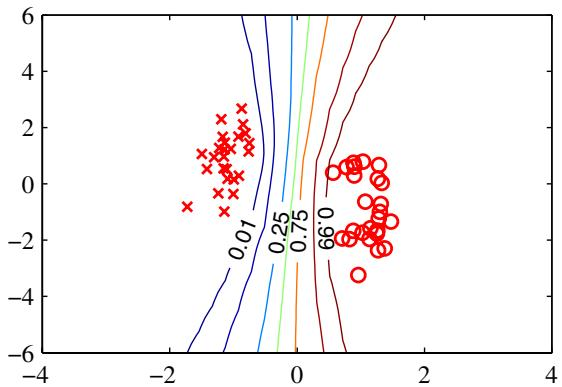
\includegraphics[keepaspectratio,alt={image}]{images/5d518c2fa238d27ecb727477ace9529b4b5326cda2a68c5df1e8f408968a0de2.jpg}}

\pandocbounded{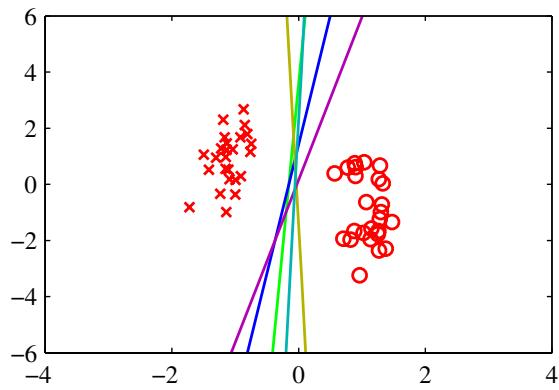
\includegraphics[keepaspectratio,alt={image}]{images/fc6e808395c68bdb581dcb9e7312ca36e25ae15dd1e9ce1e994e844febccdd52.jpg}}

Figure 10.13 Illustration of the Bayesian approach to logistic
regression for a simple linearly separable data set. The plot on the
left shows the predictive distribution obtained using variational
inference. We see that the decision boundary lies roughly mid way
between the clusters of data points, and that the contours of the
predictive distribution splay out away from the data reflecting the
greater uncertainty in the classification of such regions. The plot on
the right shows the decision boundaries corresponding to five samples of
the parameter vector w drawn from the posterior distribution
\(p ( \mathbf { w } | \mathbf { t } )\)

\[
\begin{array}{r c l} \mathcal {L} (\pmb {\xi}) & = & \frac {1}{2} \ln \frac {| \mathbf {S} _ {N} |}{| \mathbf {S} _ {0} |} - \frac {1}{2} \mathbf {m} _ {N} ^ {\mathrm{T}} \mathbf {S} _ {N} ^ {- 1} \mathbf {m} _ {N} + \frac {1}{2} \mathbf {m} _ {0} ^ {\mathrm{T}} \mathbf {S} _ {0} ^ {- 1} \mathbf {m} _ {0} \\ & & + \sum_ {n = 1} ^ {N} \left\{\ln \sigma (\xi_ {n}) - \frac {1}{2} \xi_ {n} - \lambda (\xi_ {n}) \xi_ {n} ^ {2} \right\}. \end{array}\tag{10.164}
\]

This variational framework can also be applied to situations in which
the data is arriving sequentially (Jaakkola and Jordan, 2000). In this
case we maintain a Gaussian posterior distribution over w, which is
initialized using the prior \(p ( \mathbf { w } )\) . As each data point
arrives, the posterior is updated by making use of the bound (10.151)
and then normalized to give an updated posterior distribution.

The predictive distribution is obtained by marginalizing over the
posterior distribution, and takes the same form as for the Laplace
approximation discussed in Section 4.5.2. Figure 10.13 shows the
variational predictive distributions for a synthetic data set. This
example provides interesting insights into the concept of `large
margin', which was discussed in Section 7.1 and which has qualitatively
similar behaviour to the Bayesian solution.

\subsection{10.6.3 Inference of
hyperparameters}\label{inference-of-hyperparameters}

So far, we have treated the hyperparameter α in the prior distribution
as a known constant. We now extend the Bayesian logistic regression
model to allow the value of this parameter to be inferred from the data
set. This can be achieved by combining the global and local variational
approximations into a single framework, so as to maintain a lower bound
on the marginal likelihood at each stage. Such a combined approach was
adopted by Bishop and Svensen (2003) in the context of a Bayesian ´
treatment of the hierarchical mixture of experts model.

Specifically, we consider once again a simple isotropic Gaussian prior
distribution of the form

\[
p (\mathbf {w} | \alpha) = \mathcal {N} (\mathbf {w} | \mathbf {0}, \alpha^ {- 1} \mathbf {I}).\tag{10.165}
\]

Our analysis is readily extended to more general Gaussian priors, for
instance if we wish to associate a different hyperparameter with
different subsets of the parameters \(w _ { j }\) . As usual, we
consider a conjugate hyperprior over α given by a gamma distribution

\[
p (\alpha) = \operatorname{Gam} (\alpha | a _ {0}, b _ {0})\tag{10.166}
\]

governed by the constants \(a _ { 0 }\) and \(b _ { 0 }\) .

The marginal likelihood for this model now takes the form

\[
p (\mathbf {t}) = \iint p (\mathbf {w}, \alpha , \mathbf {t}) d \mathbf {w} d \alpha\tag{10.167}
\]

where the joint distribution is given by

\[
p (\mathbf {w}, \alpha , \mathbf {t}) = p (\mathbf {t} | \mathbf {w}) p (\mathbf {w} | \alpha) p (\alpha).\tag{10.168}
\]

We are now faced with an analytically intractable integration over w and
\(\alpha ,\) which we shall tackle by using both the local and global
variational approaches in the same model

To begin with, we introduce a variational distribution
\(q ( \mathbf { w } , \alpha )\) , and then apply the decomposition
(10.2), which in this instance takes the form

\[
\ln p (\mathbf {t}) = \mathcal {L} (q) + \mathrm{KL} (q \| p)\tag{10.169}
\]

where the lower bound \(\mathcal { L } ( q )\) and the Kullback-Leibler
divergence \(\mathrm { K L } ( q \| p )\) are defined by

\[
\mathcal {L} (q) = \iint q (\mathbf {w}, \alpha) \ln \left\{\frac {p (\mathbf {w} , \alpha , \mathbf {t})}{q (\mathbf {w} , \alpha)} \right\} d \mathbf {w} d \alpha\tag{10.170}
\]

\[
\mathrm{KL} (q \| p) = - \iint q (\mathbf {w}, \alpha) \ln \left\{\frac {p (\mathbf {w} , \alpha | \mathbf {t}))}{q (\mathbf {w} , \alpha)} \right\} \mathrm{d} \mathbf {w} \mathrm{d} \alpha .\tag{10.171}
\]

At this point, the lower bound \(\mathcal { L } ( q )\) is still
intractable due to the form of the likelihood factor
\(p ( \mathbf { t } | \mathbf { w } )\) . We therefore apply the local
variational bound to each of the logistic sigmoid factors as before.
This allows us to use the inequality (10.152) and place a lower bound on
\(\mathcal { L } ( q )\) , which will therefore also be a lower bound on
the log marginal likelihood

\[
\begin{array}{r c l} \ln p (\mathbf {t}) & \geqslant & \mathcal {L} (q) \geqslant \widetilde {\mathcal {L}} (q, \boldsymbol {\xi}) \\ & = & \iint q (\mathbf {w}, \alpha) \ln \left\{\frac {h (\mathbf {w} , \boldsymbol {\xi}) p (\mathbf {w} | \alpha) p (\alpha)}{q (\mathbf {w} , \alpha)} \right\} \mathrm{d} \mathbf {w}   \mathrm{d} \alpha . \end{array}\tag{10.172}
\]

Next we assume that the variational distribution factorizes between
parameters and hyperparameters so that

\[
q (\mathbf {w}, \alpha) = q (\mathbf {w}) q (\alpha).\tag{10.173}
\]

With this factorization we can appeal to the general result (10.9) to
find expressions for the optimal factors. Consider first the
distribution \(q ( \mathbf { w } )\) . Discarding terms that are
independent of w, we have

\[
\begin{array}{r c l} \ln q (\mathbf {w}) & = & \mathbb {E} _ {\alpha} \left[ \ln \left\{h (\mathbf {w}, \pmb {\xi}) p (\mathbf {w} | \alpha) p (\alpha) \right\} \right] + \mathrm{const} \\ & = & \ln h (\mathbf {w}, \pmb {\xi}) + \mathbb {E} _ {\alpha} \left[ \ln p (\mathbf {w} | \alpha) \right] + \mathrm{const}. \end{array}
\]

We now substitute for ln \(h ( \mathbf { w } , \pmb { \xi } )\) using
(10.153), and for ln \(p ( \mathbf { w } | \alpha )\) using (10.165),
giving

\[
\ln q (\mathbf {w}) = - \frac {\mathbb {E} [ \alpha ]}{2} \mathbf {w} ^ {\mathrm{T}} \mathbf {w} + \sum_ {n = 1} ^ {N} \left\{(t _ {n} - 1 / 2) \mathbf {w} ^ {\mathrm{T}} \boldsymbol {\phi} _ {n} - \lambda (\xi_ {n}) \mathbf {w} ^ {\mathrm{T}} \boldsymbol {\phi} _ {n} \boldsymbol {\phi} _ {n} ^ {\mathrm{T}} \mathbf {w} \right\} + \mathrm{const.}
\]

We see that this is a quadratic function of w and so the solution for
\(q ( \mathbf { w } )\) will be Gaussian. Completing the square in the
usual way, we obtain

\[
q (\mathbf {w}) = \mathcal {N} (\mathbf {w} | \boldsymbol {\mu} _ {N}, \boldsymbol {\Sigma} _ {N})\tag{10.174}
\]

where we have defined

\[
\boldsymbol {\Sigma} _ {N} ^ {- 1} \boldsymbol {\mu} _ {N} = \sum_ {n = 1} ^ {N} (t _ {n} - 1 / 2) \phi_ {n}\tag{10.175}
\]

\[
\boldsymbol {\Sigma} _ {N} ^ {- 1} = \mathbb {E} [ \alpha ] \mathbf {I} + 2 \sum_ {n = 1} ^ {N} \lambda (\xi_ {n}) \boldsymbol {\phi} _ {n} \boldsymbol {\phi} _ {n} ^ {\mathrm{T}}.\tag{10.176}
\]

Similarly, the optimal solution for the factor \(q ( \alpha )\) is
obtained from

\[
\ln q (\alpha) = \mathbb {E} _ {\mathbf {w}} \left[ \ln p (\mathbf {w} | \alpha) \right] + \ln p (\alpha) + \mathrm{const.}
\]

Substituting for ln \(p ( \mathbf { w } | \alpha )\) using (10.165), and
for ln \(p ( \alpha )\) using (10.166), we obtain

\[
\ln q (\alpha) = \frac {M}{2} \ln \alpha - \frac {\alpha}{2} \mathbb {E} \left[ \mathbf {w} ^ {\mathrm{T}} \mathbf {w} \right] + (a _ {0} - 1) \ln \alpha - b _ {0} \alpha + \mathrm{const}.
\]

We recognize this as the log of a gamma distribution, and so we obtain

\[
q (\alpha) = \operatorname{Gam} (\alpha | a _ {N}, b _ {N}) = \frac {1}{\Gamma (a _ {0})} a _ {0} ^ {b _ {0}} \alpha^ {a _ {0} - 1} e ^ {- b _ {0} \alpha}\tag{10.177}
\]

where

\[
a _ {N} = a _ {0} + \frac {M}{2}\tag{10.178}
\]

\[
{b _ {N}} = {b _ {0} + \frac {1}{2} \mathbb {E} _ {\mathbf {w}} \left[ \mathbf {w} ^ {\mathrm{T}} \mathbf {w} \right].}\tag{10.179}
\]

We also need to optimize the variational parameters \(\xi _ { n }\) ,
and this is also done by maximizing the lower bound
\(\widetilde { \mathcal { L } } ( q , \xi )\) . Omitting terms that are
independent of \(\xi ,\) and integrating over α, we have

\[
\widetilde {\mathcal {L}} (q, \pmb {\xi}) = \int q (\mathbf {w}) \ln h (\mathbf {w}, \pmb {\xi}) \mathrm{d} \mathbf {w} + \mathrm{const}.\tag{10.180}
\]

Note that this has precisely the same form as (10.159), and so we can
again appeal to our earlier result (10.163), which can be obtained by
direct optimization of the marginal likelihood function, leading to
re-estimation equations of the form

\[
(\xi_ {n} ^ {\mathrm{new}}) ^ {2} = \phi_ {n} ^ {\mathrm{T}} (\pmb {\Sigma} _ {N} + \pmb {\mu} _ {N} \pmb {\mu} _ {N} ^ {\mathrm{T}}) \phi_ {n}.\tag{10.181}
\]

We have obtained re-estimation equations for the three quantities
\(q ( \mathbf { w } ) , q ( \alpha )\) and \(\xi ,\) , and so after
making suitable initializations, we can cycle through these quantities,
updating each in turn. The required moments are given by

Appendix B

\[
\mathbb {E} [ \alpha ] = \frac {a _ {N}}{b _ {N}}\tag{10.182}
\]

\[
{\mathbb {E} \left[ \mathbf {w} ^ {\mathrm{T}} \mathbf {w} \right]} = {\boldsymbol {\Sigma} _ {N} + \boldsymbol {\mu} _ {N} ^ {\mathrm{T}} \boldsymbol {\mu} _ {N}.}\tag{10.183}
\]

\subsection{10.7. Expectation
Propagation}\label{expectation-propagation}

We conclude this chapter by discussing an alternative form of
deterministic approximate inference, known as expectation propagation or
\(E P\) (Minka, 2001a; Minka, 2001b). As with the variational Bayes
methods discussed so far, this too is based on the minimization of a
Kullback-Leibler divergence but now of the reverse form, which gives the
approximation rather different properties.

Consider for a moment the problem of minimizing KL \(( p \| q )\) with
respect to \(q ( \mathbf { z } )\) when \(p ( \mathbf { z } )\) is a
fixed distribution and \(q ( \mathbf { z } )\) is a member of the
exponential family and so, from (2.194), can be written in the form

\[
q (\mathbf {z}) = h (\mathbf {z}) g (\boldsymbol {\eta}) \exp \left\{\boldsymbol {\eta} ^ {\mathrm{T}} \mathbf {u} (\mathbf {z}) \right\}.\tag{10.184}
\]

As a function of \(\eta ,\) the Kullback-Leibler divergence then becomes

\[
\mathrm{KL} (p \| q) = - \ln g (\pmb {\eta}) - \pmb {\eta} ^ {\mathrm{T}} \mathbb {E} _ {p (\mathbf {z})} [ \mathbf {u} (\mathbf {z}) ] + \mathrm{const}\tag{10.185}
\]

where the constant terms are independent of the natural parameters
\(\eta .\) . We can minimize \(\mathrm { K L } ( p | | q )\) within this
family of distributions by setting the gradient with respect to η to
zero, giving

\[
- \nabla \ln g (\boldsymbol {\eta}) = \mathbb {E} _ {p (\mathbf {z})} [ \mathbf {u} (\mathbf {z}) ].\tag{10.186}
\]

However, we have already seen in (2.226) that the negative gradient of
ln \(g ( \pmb { \eta } )\) is given by the expectation of
\(\mathbf { u } ( \mathbf { z } )\) under the distribution
\(q ( \mathbf { z } )\) . Equating these two results, we obtain

\[
\mathbb {E} _ {q (\mathbf {z})} [ \mathbf {u} (\mathbf {z}) ] = \mathbb {E} _ {p (\mathbf {z})} [ \mathbf {u} (\mathbf {z}) ].\tag{10.187}
\]

We see that the optimum solution simply corresponds to matching the
expected sufficient statistics. So, for instance, if
\(q ( \mathbf { z } )\) is a Gaussian
\(\mathcal { N } ( \mathbf { z } | \boldsymbol { \mu } , \boldsymbol { \Sigma } )\)
then we minimize the Kullback-Leibler divergence by setting the mean
\(\pmb { \mu }\) of \(q ( \mathbf { z } )\) equal to the mean of the
distribution \(p ( \mathbf { z } )\) and the covariance
\(\bar { \Sigma }\) equal to the covariance of \(p ( \mathbf { z } )\) .
This is sometimes called moment matching. An example of this was seen in
Figure 10.3(a).

Now let us exploit this result to obtain a practical algorithm for
approximate inference. For many probabilistic models, the joint
distribution of data \(\mathcal { D }\) and hidden variables (including
parameters) \(\pmb \theta\) comprises a product of factors in the form

\[
p (\mathcal {D}, \boldsymbol {\theta}) = \prod_ {i} f _ {i} (\boldsymbol {\theta}).\tag{10.188}
\]

This would arise, for example, in a model for independent, identically
distributed data in which there is one factor
\(f _ { n } ( \pmb { \theta } ) = p ( \mathbf { x } _ { n } | \pmb { \theta } )\)
for each data point \({ \bf x } _ { n }\) , along with a factor
\(f _ { 0 } ( \pmb { \theta } ) = p ( \pmb { \theta } )\) corresponding
to the prior. More generally, it would also apply to any model defined
by a directed probabilistic graph in which each factor is a conditional
distribution corresponding to one of the nodes, or an undirected graph
in which each factor is a clique potential. We are interested in
evaluating the posterior distribution
\(p ( \pmb \theta | \mathcal { D } )\) for the purpose of making
predictions, as well as the model evidence \(p ( \mathcal { D } )\) for
the purpose of model comparison. From (10.188) the posterior is given by

\[
p (\pmb {\theta} | \mathcal {D}) = \frac {1}{p (\mathcal {D})} \prod_ {i} f _ {i} (\pmb {\theta})\tag{10.189}
\]

and the model evidence is given by

\[
p (\mathcal {D}) = \int \prod_ {i} f _ {i} (\boldsymbol {\theta}) \mathrm{d} \boldsymbol {\theta}.\tag{10.190}
\]

Here we are considering continuous variables, but the following
discussion applies equally to discrete variables with integrals replaced
by summations. We shall suppose that the marginalization over
\(\theta ,\) , along with the marginalizations with respect to the
posterior distribution required to make predictions, are intractable so
that some form of approximation is required.

Expectation propagation is based on an approximation to the posterior
distribution which is also given by a product of factors

\[
q (\pmb {\theta}) = \frac {1}{Z} \prod_ {i} \widetilde {f} _ {i} (\pmb {\theta})\tag{10.191}
\]

in which each factor \(\widetilde { f } _ { i } ( \pmb \theta )\) in the
approximation corresponds to one of the factors
\(f _ { i } ( \pmb \theta )\) in the true posterior (10.189), and the
factor \(1 / Z\) is the normalizing constant needed to ensure that the
left-hand side of (10.191) integrates to unity. In order to obtain a
practical algorithm, we need to constrain the factors
\(\widetilde { f } _ { i } ( \pmb \theta )\) in some way, and in
particular we shall assume that they come from the exponential family.
The product of the factors will therefore also be from the exponential
family and so can be described by a finite set of sufficient statistics.
For example, if each of the \(\widetilde { f } _ { i } ( \pmb \theta )\)
is a Gaussian, then the overall approximation \(q ( \pmb \theta )\) will
also be Gaussian.

Ideally we would like to determine the
\(\widetilde { f } _ { i } ( \pmb \theta )\) by minimizing the
Kullback-Leibler divergence between the true posterior and the
approximation given by

\[
\mathrm{KL} \left(p \| q\right) = \mathrm{KL} \left(\frac {1}{p (\mathcal {D})} \prod_ {i} f _ {i} (\boldsymbol {\theta}) \Bigg | \Bigg | \frac {1}{Z} \prod_ {i} \widetilde {f} _ {i} (\boldsymbol {\theta})\right).\tag{10.192}
\]

Note that this is the reverse form of KL divergence compared with that
used in variational inference. In general, this minimization will be
intractable because the KL divergence involves averaging with respect to
the true distribution. As a rough approximation, we could instead
minimize the KL divergences between the corresponding pairs
\(f _ { i } ( \pmb \theta )\) and
\(\widetilde { f } _ { i } ( \pmb \theta )\) of factors. This represents
a much simpler problem to solve, and has the advantage that the
algorithm is noniterative. However, because each factor is individually
approximated, the product of the factors could well give a poor
approximation.

Expectation propagation makes a much better approximation by optimizing
each factor in turn in the context of all of the remaining factors. It
starts by initializing the factors
\(\widetilde { f } _ { i } ( \pmb \theta )\) , and then cycles through
the factors refining them one at a time. This is similar in spirit to
the update of factors in the variational Bayes framework considered
earlier. Suppose we wish to refine factor
\(\widetilde { f } _ { j } ( \pmb { \theta } )\) . We first remove this
factor from the product to give
\(\textstyle \prod _ { i \neq j } { \widetilde { f } } _ { i } ( \pmb \theta )\)
. Conceptually, we will now determine a revised form of the factor
\(\widetilde { f } _ { j } ( \pmb { \theta } )\) by ensuring that the
product

\[
q ^ {\mathrm{new}} (\boldsymbol {\theta}) \propto \widetilde {f} _ {j} (\boldsymbol {\theta}) \prod_ {i \neq j} \widetilde {f} _ {i} (\boldsymbol {\theta})\tag{10.193}
\]

is as close as possible to

\[
f _ {j} (\boldsymbol {\theta}) \prod_ {i \neq j} \widetilde {f} _ {i} (\boldsymbol {\theta})\tag{10.194}
\]

in which we keep fixed all of the factors
\(\widetilde { f } _ { i } ( \pmb \theta )\) for \(i \neq j\) . This
ensures that the approximation is most accurate in the regions of high
posterior probability as defined by the remaining factors. We shall see
an example of this effect when we apply EP to the `clutter problem'. To
achieve this, we first remove the factor
\(\widetilde { f } _ { j } ( \pmb { \theta } )\) from the current
approximation to the posterior by defining the unnormalized distribution

\[
q ^ {\backslash j} (\boldsymbol {\theta}) = \frac {q (\boldsymbol {\theta})}{\widetilde {f} _ {j} (\boldsymbol {\theta})}.\tag{10.195}
\]

Note that we could instead find \(q ^ { \setminus j } ( \pmb \theta )\)
from the product of factors \(i \neq j\) , although in practice division
is usually easier. This is now combined with the factor
\(f _ { j } ( \pmb \theta )\) to give a distribution

\[
\frac {1}{Z _ {j}} f _ {j} (\pmb {\theta}) q ^ {\backslash j} (\pmb {\theta})\tag{10.196}
\]

\pandocbounded{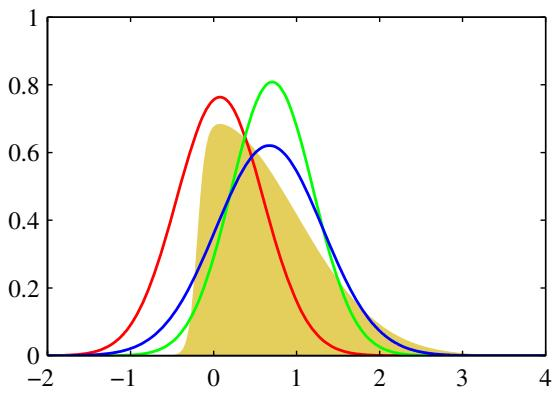
\includegraphics[keepaspectratio,alt={image}]{images/e25781cc01cbbc14d466198706fa2ccdad2e2601fb54341bf8245562f6077513.jpg}}

\pandocbounded{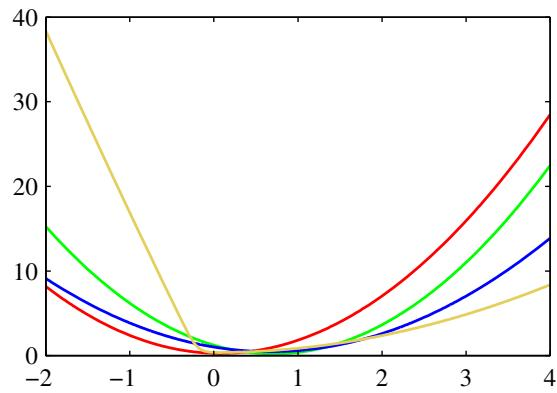
\includegraphics[keepaspectratio,alt={image}]{images/62c279a61c993b7c83b65f59532ddb2f8dc7048932d507a77e73e8df7195fe4c.jpg}}

Figure 10.14 Illustration of the expectation propagation approximation
using a Gaussian distribution for the example considered earlier in
Figures 4.14 and 10.1. The left-hand plot shows the original
distribution (yellow) along with the Laplace (red), global variational
(green), and EP (blue) approximations, and the right-hand plot shows the
corresponding negative logarithms of the distributions. Note that the
\(\mathsf { E P }\) distribution is broader than that variational
inference, as a consequence of the different form of KL divergence.

where \(Z _ { j }\) is the normalization constant given by

\[
Z _ {j} = \int f _ {j} (\boldsymbol {\theta}) q ^ {\backslash j} (\boldsymbol {\theta}) \mathrm{d} \boldsymbol {\theta}.\tag{10.197}
\]

We now determine a revised factor
\(\widetilde { f } _ { j } ( \pmb { \theta } )\) by minimizing the
Kullback-Leibler divergence

\[
\mathrm{KL} \left( \right.\frac {f _ {j} (\boldsymbol {\theta}) q ^ {\backslash j} (\boldsymbol {\theta})}{Z _ {j}} \left. \right\| q ^ {\text { new }} (\boldsymbol {\theta})\left. \right).\tag{10.198}
\]

This is easily solved because the approximating distribution
\(q ^ { \mathrm { n e w } } ( \pmb { \theta } )\) is from the
exponential family, and so we can appeal to the result (10.187), which
tells us that the parameters of
\(q ^ { \mathrm { n e w } } ( \pmb { \theta } )\) are obtained by
matching its expected sufficient statistics to the corresponding moments
of (10.196). We shall assume that this is a tractable operation. For
example, if we choose \(q ( \pmb \theta )\) to be a Gaussian
distribution
\(\mathcal { N } ( \pmb { \theta } | \pmb { \mu } , \pmb { \Sigma } )\)
, then \(\pmb { \mu }\) is set equal to the mean of the (unnormalized)
distribution
\(f _ { j } ( \pmb { \theta } ) q ^ { \backslash j } ( \pmb { \theta } )\)
, and Σ is set to its covariance. More generally, it is straightforward
to obtain the required expectations for any member of the exponential
family, provided it can be normalized, because the expected statistics
can be related to the derivatives of the normalization coefficient, as
given by (2.226). The EP approximation is illustrated in Figure 10.14.

From (10.193), we see that the revised factor
\(\widetilde { f } _ { j } ( \pmb { \theta } )\) can be found by taking
\(q ^ { \mathrm { n e w } } ( \pmb { \theta } )\) and dividing out the
remaining factors so that

\[
\widetilde {f} _ {j} (\boldsymbol {\theta}) = K \frac {q ^ {\text { new }} (\boldsymbol {\theta})}{q ^ {\backslash j} (\boldsymbol {\theta})}\tag{10.199}
\]

where we have used (10.195). The coefficient K is determined by
multiplying both

sides of (10.199) by \(q ^ { \backslash i } ( \pmb \theta )\) and
integrating to give

\[
K = \int \widetilde {f} _ {j} (\boldsymbol {\theta}) q ^ {\backslash j} (\boldsymbol {\theta}) \mathrm{d} \boldsymbol {\theta}\tag{10.200}
\]

where we have used the fact that
\(q ^ { \mathrm { n e w } } ( \pmb { \theta } )\) is normalized. The
value of K can therefore be found by matching zeroth-order moments

\[
\int \widetilde {f} _ {j} (\boldsymbol {\theta}) q ^ {\backslash j} (\boldsymbol {\theta}) \mathrm{d} \boldsymbol {\theta} = \int f _ {j} (\boldsymbol {\theta}) q ^ {\backslash j} (\boldsymbol {\theta}) \mathrm{d} \boldsymbol {\theta}.\tag{10.201}
\]

Combining this with (10.197), we then see that \(K = Z _ { j }\) and so
can be found by evaluating the integral in (10.197).

In practice, several passes are made through the set of factors,
revising each factor in turn. The posterior distribution
\(p ( \pmb \theta | \mathcal { D } )\) is then approximated using
(10.191), and the model evidence \(p ( \mathcal { D } )\) can be
approximated by using (10.190) with the factors
\(f _ { i } ( \pmb \theta )\) replaced by their approximations
\(\widetilde { f } _ { i } ( \pmb \theta )\)

\subsection{Expectation Propagation}\label{expectation-propagation-1}

We are given a joint distribution over observed data \(\mathcal { D }\)
and stochastic variables θ in the form of a product of factors

\[
p (\mathcal {D}, \boldsymbol {\theta}) = \prod_ {i} f _ {i} (\boldsymbol {\theta})\tag{10.202}
\]

and we wish to approximate the posterior distribution
\(p ( \pmb \theta | \mathcal { D } )\) by a distribution of the form 1

\[
q (\pmb {\theta}) = \frac {1}{Z} \prod_ {i} \widetilde {f} _ {i} (\pmb {\theta}).\tag{10.203}
\]

We also wish to approximate the model evidence \(p ( \mathcal { D } )\)

\begin{enumerate}
\def\labelenumi{\arabic{enumi}.}
\tightlist
\item
  Initialize all of the approximating factors
  \(\widetilde { f } _ { i } ( \pmb \theta )\)
\end{enumerate}

2. Initialize the posterior approximation by setting

\[
q (\boldsymbol {\theta}) \propto \prod_ {i} \widetilde {f} _ {i} (\boldsymbol {\theta}).\tag{10.204}
\]

\begin{enumerate}
\def\labelenumi{\arabic{enumi}.}
\setcounter{enumi}{2}
\tightlist
\item
  Until convergence:
\end{enumerate}

\begin{enumerate}
\def\labelenumi{(\alph{enumi})}
\item
  Choose a factor \(\widetilde { f } _ { j } ( \pmb { \theta } )\) to
  refine.
\item
  Remove \(\widetilde { f } _ { j } ( \pmb { \theta } )\) from the
  posterior by division
\end{enumerate}

\[
q ^ {\backslash j} (\boldsymbol {\theta}) = \frac {q (\boldsymbol {\theta})}{\widetilde {f} _ {j} (\boldsymbol {\theta})}.\tag{10.205}
\]

\begin{enumerate}
\def\labelenumi{(\alph{enumi})}
\setcounter{enumi}{2}
\tightlist
\item
  Evaluate the new posterior by setting the sufficient statistics
  (moments) of \(q ^ { \mathrm { n e w } } ( \pmb { \theta } )\) equal
  to those of
  \(q ^ { \setminus j } ( { \pmb \theta } ) { \overline { { f _ { j } } } } ( { \pmb \theta } )\)
  , including evaluation of the normalization constant
\end{enumerate}

\[
Z _ {j} = \int q ^ {\backslash j} (\boldsymbol {\theta}) f _ {j} (\boldsymbol {\theta}) \mathrm{d} \boldsymbol {\theta}.\tag{10.206}
\]

\begin{enumerate}
\def\labelenumi{(\alph{enumi})}
\setcounter{enumi}{3}
\tightlist
\item
  Evaluate and store the new factor
\end{enumerate}

\[
\widetilde {f} _ {j} (\boldsymbol {\theta}) = Z _ {j} \frac {q ^ {\mathrm{new}} (\boldsymbol {\theta})}{q ^ {\backslash j} (\boldsymbol {\theta})}.\tag{10.207}
\]

\begin{enumerate}
\def\labelenumi{\arabic{enumi}.}
\setcounter{enumi}{3}
\tightlist
\item
  Evaluate the approximation to the model evidence
\end{enumerate}

\[
p (\mathcal {D}) \simeq \int \prod_ {i} \widetilde {f} _ {i} (\boldsymbol {\theta}) \mathrm{d} \boldsymbol {\theta}.\tag{10.208}
\]

A special case of EP, known as assumed density filtering (ADF) or moment
matching (Maybeck, 1982; Lauritzen, 1992; Boyen and Koller, 1998; Opper
and Winther, 1999), is obtained by initializing all of the approximating
factors except the first to unity and then making one pass through the
factors updating each of them once. Assumed density filtering can be
appropriate for on-line learning in which data points are arriving in a
sequence and we need to learn from each data point and then discard it
before considering the next point. However, in a batch setting we have
the opportunity to re-use the data points many times in order to achieve
improved accuracy, and it is this idea that is exploited in expectation
propagation. Furthermore, if we apply ADF to batch data, the results
will have an undesirable dependence on the (arbitrary) order in which
the data points are considered, which again EP can overcome.

One disadvantage of expectation propagation is that there is no
guarantee that the iterations will converge. However, for approximations
\(q ( \pmb \theta )\) in the exponential family, if the iterations do
converge, the resulting solution will be a stationary point of a
particular energy function (Minka, 2001a), although each iteration of EP
does not necessarily decrease the value of this energy function. This is
in contrast to variational Bayes, which iteratively maximizes a lower
bound on the log marginal likelihood, in which each iteration is
guaranteed not to decrease the bound. It is possible to optimize the EP
cost function directly, in which case it is guaranteed to converge,
although the resulting algorithms can be slower and more complex to
implement.

Another difference between variational Bayes and EP arises from the form
of KL divergence that is minimized by the two algorithms, because the
former minimizes \(\operatorname { K L } ( q \| p )\) whereas the latter
minimizes \(\mathrm { K L } ( p \Vert q )\) . As we saw in Figure 10.3,
for distributions \(p ( \pmb \theta )\) which are multimodal, minimizing
\(\mathrm { K L } ( p | | q )\) can lead to poor approximations. In
particular, if EP is applied to mixtures the results are not sensible
because the approximation tries to capture all of the modes of the
posterior distribution. Conversely, in logistic-type models, EP often
out-performs both local variational methods and the Laplace
approximation (Kuss and Rasmussen, 2006).

Figure 10.15

Illustration of the clutter problem for a data space dimensionality of
\(D = 1\) Training data points, denoted by the crosses, are drawn from a
mixture of two Gaussians with components shown in red and green. The
goal is to infer the mean of the green Gaussian from the observed data.

\pandocbounded{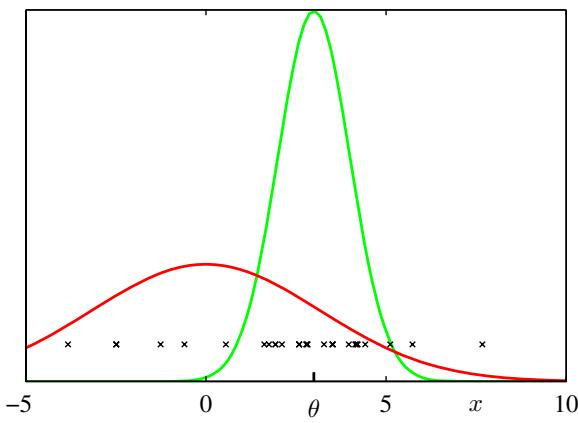
\includegraphics[keepaspectratio,alt={image}]{images/ce06932e99b8206063210b7b216fc0f554b88ffbdef0b3a2552b727d37e5e375.jpg}}

\subsection{10.7.1 Example: The clutter
problem}\label{example-the-clutter-problem}

Following Minka (2001b), we illustrate the EP algorithm using a simple
example in which the goal is to infer the mean \(\pmb \theta\) of a
multivariate Gaussian distribution over a variable x given a set of
observations drawn from that distribution. To make the problem more
interesting, the observations are embedded in background clutter, which
itself is also Gaussian distributed, as illustrated in Figure 10.15. The
distribution of observed values x is therefore a mixture of Gaussians,
which we take to be of the form

\[
p (\mathbf {x} | \boldsymbol {\theta}) = (1 - w) \mathcal {N} (\mathbf {x} | \boldsymbol {\theta}, \mathbf {I}) + w \mathcal {N} (\mathbf {x} | \mathbf {0}, a \mathbf {I})\tag{10.209}
\]

where \(w\) is the proportion of background clutter and is assumed to be
known. The prior over \(\pmb \theta\) is taken to be Gaussian

\[
p (\boldsymbol {\theta}) = \mathcal {N} (\boldsymbol {\theta} | \mathbf {0}, b \mathbf {I})\tag{10.210}
\]

and Minka (2001a) chooses the parameter values \(a = 1 0 , b = 1 0 0\)
and \(w = 0 . 5\) The joint distribution of N observations
\(\mathcal { D } = \{ \mathbf { x } _ { 1 } , \ldots , \mathbf { x } _ { N } \}\)
and θ is given by

\[
p (\mathcal {D}, \pmb {\theta}) = p (\pmb {\theta}) \prod_ {n = 1} ^ {N} p (\mathbf {x} _ {n} | \pmb {\theta})\tag{10.211}
\]

and so the posterior distribution comprises a mixture of \(2 ^ { N }\)
Gaussians. Thus the computational cost of solving this problem exactly
would grow exponentially with the size of the data set, and so an exact
solution is intractable for moderately large \(N\)

To apply EP to the clutter problem, we first identify the factors
\(f _ { 0 } ( \pmb { \theta } ) = p ( \pmb { \theta } )\) and
\(f _ { n } ( \pmb { \theta } ) = p ( \mathbf x _ { n } | \pmb \theta )\)
. Next we select an approximating distribution from the exponential
family, and for this example it is convenient to choose a spherical
Gaussian

\[
q (\boldsymbol {\theta}) = \mathcal {N} (\boldsymbol {\theta} | \mathbf {m}, v \mathbf {I}).\tag{10.212}
\]

The factor approximations will therefore take the form of
exponential-quadratic functions of the form

\[
\widetilde {f} _ {n} (\pmb {\theta}) = s _ {n} \mathcal {N} (\pmb {\theta} | \mathbf {m} _ {n}, v _ {n} \mathbf {I})\tag{10.213}
\]

where \(n = 1 , \ldots , N\) , and we set
\(\widetilde { f } _ { 0 } ( \pmb { \theta } )\) equal to the prior
\(p ( \pmb \theta )\) . Note that the use of
\(\mathcal { N } ( \pmb \theta | \cdot , \cdot )\) does not imply that
the right-hand side is a well-defined Gaussian density (in fact, as we
shall see, the variance parameter \(v _ { n }\) can be negative) but is
simply a convenient shorthand notation. The approximations
\({ \widetilde { f } } _ { n } ( \pmb \theta )\) , for
\(n = 1 , \ldots , N\) , can be initialized to unity, corresponding to
\(s _ { n } = ( 2 \pi v _ { n } ) ^ { D / 2 } , v _ { n } \to \infty\)
and \(\mathbf { m } _ { n } = \mathbf { 0 }\) where \(D\) is the
dimensionality of x and hence of \(\pmb { \theta } .\) . The initial
\(q ( \pmb \theta )\) , defined by (10.191), is therefore equal to the
prior.

We then iteratively refine the factors by taking one factor
\(f _ { n } ( \pmb \theta )\) at a time and applying (10.205), (10.206),
and (10.207). Note that we do not need to revise the term
\(f _ { 0 } ( \pmb { \theta } )\) because an EP update will leave this
term unchanged. Here we state the results and leave the reader to fill
in the details.

First we remove the current estimate
\({ \dot { f } } _ { n } ( \pmb { \theta } )\) from
\(q ( \pmb \theta )\) by division using (10.205) to give
\(q ^ { \setminus n } ( \pmb \theta )\) , which has mean and inverse
variance given by

\[
{\mathbf m} ^ {\backslash n} = {\mathbf m} + v ^ {\backslash n} v _ {n} ^ {- 1} ({\mathbf m} - {\mathbf m} _ {n})\tag{10.214}
\]

\[
(v ^ {\backslash n}) ^ {- 1} = v ^ {- 1} - v _ {n} ^ {- 1}.\tag{10.215}
\]

Next we evaluate the normalization constant \(Z _ { n }\) using (10.206)
to give

\[
Z _ {n} = (1 - w) \mathcal {N} (\mathbf {x} _ {n} | \mathbf {m} ^ {\backslash n}, (v ^ {\backslash n} + 1) \mathbf {I}) + w \mathcal {N} (\mathbf {x} _ {n} | \mathbf {0}, a \mathbf {I}).\tag{10.216}
\]

Similarly, we compute the mean and variance of
\(q ^ { \mathrm { n e w } } ( \pmb { \theta } )\) by finding the mean
and variance of
\(q ^ { \backslash n } ( \pmb \theta ) \bar { f } _ { n } ( \pmb \theta )\)
to give

\[
\mathbf {m} = \mathbf {m} ^ {\backslash n} + \rho_ {n} \frac {v ^ {\backslash n}}{v ^ {\backslash n} + 1} (\mathbf {x} _ {n} - \mathbf {m} ^ {\backslash n})\tag{10.217}
\]

\[
v = v ^ {\backslash n} - \rho_ {n} \frac {(v ^ {\backslash n}) ^ {2}}{v ^ {\backslash n} + 1} + \rho_ {n} (1 - \rho_ {n}) \frac {(v ^ {\backslash n}) ^ {2} \| \mathbf {x} _ {n} - \mathbf {m} ^ {\backslash n} \| ^ {2}}{D (v ^ {\backslash n} + 1) ^ {2}}\tag{10.218}
\]

where the quantity

\[
\rho_ {n} = 1 - \frac {w}{Z _ {n}} \mathcal {N} (\mathbf {x} _ {n} | \mathbf {0}, a \mathbf {I})\tag{10.219}
\]

has a simple interpretation as the probability of the point
\({ \bf x } _ { n }\) not being clutter. Then we use (10.207) to compute
the refined factor \(\widetilde { f } _ { n } ( \pmb { \theta } )\)
whose parameters are given by

\[
{v _ {n} ^ {- 1}} = {(v ^ {\mathrm{new}}) ^ {- 1} - (v ^ {\backslash n}) ^ {- 1}}\tag{10.220}
\]

\[
\mathbf {m} _ {n} = \mathbf {m} ^ {\backslash n} + (v _ {n} + v ^ {\backslash n}) (v ^ {\backslash n}) ^ {- 1} (\mathbf {m} ^ {\mathrm{new}} - \mathbf {m} ^ {\backslash n})\tag{10.221}
\]

\[
Z _ {n}
\]

\[
{s _ {n}} = {\frac {n}{(2 \pi v _ {n}) ^ {D / 2} \mathcal {N} (\mathbf {m} _ {n} | \mathbf {m} ^ {\backslash n} , (v _ {n} + v ^ {\backslash n}) \mathbf {I})}.}\tag{10.222}
\]

This refinement process is repeated until a suitable termination
criterion is satisfied, for instance that the maximum change in
parameter values resulting from a complete pass through all factors is
less than some threshold. Finally, we use (10.208) to evaluate the
approximation to the model evidence, given by

\pandocbounded{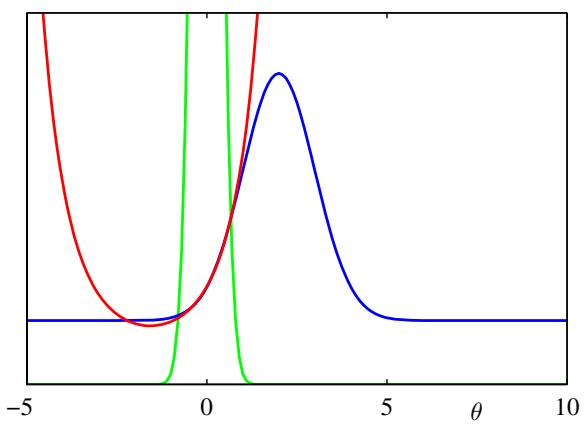
\includegraphics[keepaspectratio,alt={image}]{images/f290d67a2c42c4f82ccd2f498acc78947ad17e90da2c70e9bf33d0f92e637174.jpg}}

\pandocbounded{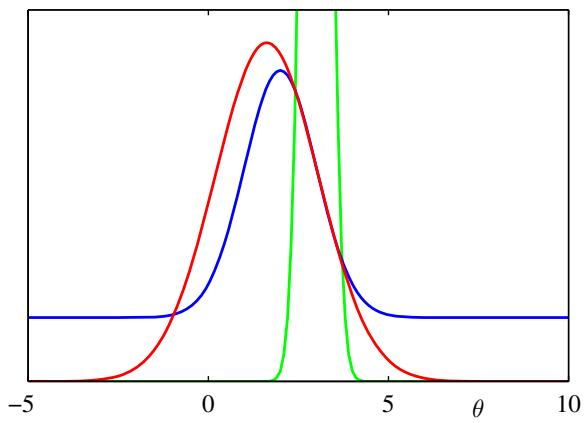
\includegraphics[keepaspectratio,alt={image}]{images/0cf60405cbeb9b71aedcb5260d7d1d4fe9a15b4027e02f314d3944356cf9a115.jpg}}

Figure 10.16 Examples of the approximation of specific factors for a
one-dimensional version of the clutter problem, showing
\(f _ { n } ( \theta )\) in blue,
\({ \widetilde { f } } _ { n } ( \theta )\) in red, and
\(q ^ { \setminus n } ( \theta )\) in green. Notice that the current
form for \(q ^ { \setminus n } ( \theta )\) controls the range of θ over
which \({ \widetilde { f } } _ { n } ( \theta )\) will be a good
approximation to \(f _ { n } ( \theta )\)

\[
p (\mathcal {D}) \simeq (2 \pi v ^ {\mathrm{new}}) ^ {D / 2} \exp (B / 2) \prod_ {n = 1} ^ {N} \left\{s _ {n} (2 \pi v _ {n}) ^ {- D / 2} \right\}\tag{10.223}
\]

where

\[
B = \frac {(\mathbf {m} ^ {\mathrm{new}}) ^ {\mathrm{T}} \mathbf {m} ^ {\mathrm{new}}}{v} - \sum_ {n = 1} ^ {N} \frac {\mathbf {m} _ {n} ^ {\mathrm{T}} \mathbf {m} _ {n}}{v _ {n}}.\tag{10.224}
\]

Examples factor approximations for the clutter problem with a
one-dimensional parameter space \(\theta\) are shown in Figure 10.16.
Note that the factor approximations can have infinite or even negative
values for the `variance' parameter \(v _ { n }\) . This simply
corresponds to approximations that curve upwards instead of downwards
and are not necessarily problematic provided the overall approximate
posterior \(q ( \pmb \theta )\) has positive variance. Figure 10.17
compares the performance of EP with variational Bayes (mean field
theory) and the Laplace approximation on the clutter problem.

\subsection{10.7.2 Expectation propagation on
graphs}\label{expectation-propagation-on-graphs}

So far in our general discussion of EP, we have allowed the factors
\(f _ { i } ( \pmb \theta )\) in the distribution \(p ( \pmb \theta )\)
to be functions of all of the components of θ, and similarly for the
approximating factors \(\widetilde f ( \pmb \theta )\) in the
approximating distribution \(q ( \pmb \theta )\) . We now consider
situations in which the factors depend only on subsets of the variables.
Such restrictions can be conveniently expressed using the framework of
probabilistic graphical models, as discussed in Chapter 8. Here we use a
factor graph representation because this encompasses both directed and
undirected graphs.

\pandocbounded{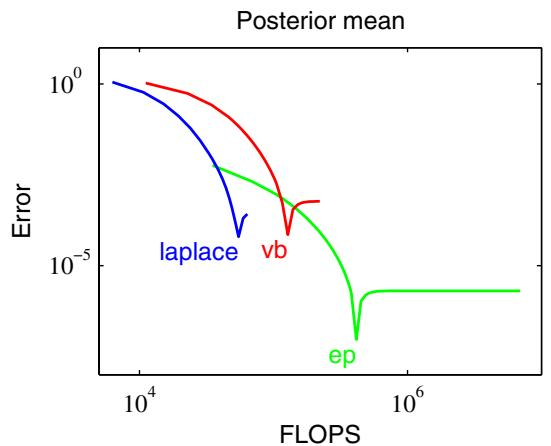
\includegraphics[keepaspectratio,alt={image}]{images/f2d0ac4f3a5f0cb9e57d583d72b083f3bff9296041fef8b6dbf4a5469b13069a.jpg}}

\pandocbounded{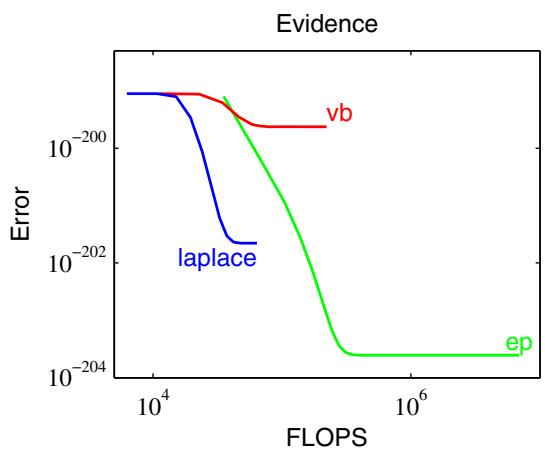
\includegraphics[keepaspectratio,alt={image}]{images/da9a3c13caf889f046a444e4d82f830f881555dfc71be3234285ba8c2e94379d.jpg}}

Figure 10.17 Comparison of expectation propagation, variational
inference, and the Laplace approximation on the clutter problem. The
left-hand plot shows the error in the predicted posterior mean versus
the number of floating point operations, and the right-hand plot shows
the corresponding results for the model evidence.

We shall focus on the case in which the approximating distribution is
fully factorized, and we shall show that in this case expectation
propagation reduces to loopy belief propagation (Minka, 2001a). To start
with, we show this in the context of a simple example, and then we shall
explore the general case.

First of all, recall from (10.17) that if we minimize the
Kullback-Leibler divergence KL \(( p \| q )\) with respect to a
factorized distribution \(q ,\) then the optimal solution for each
factor is simply the corresponding marginal of \(p .\)

Now consider the factor graph shown on the left in Figure 10.18, which
was introduced earlier in the context of the sum-product algorithm. The
joint distribution is given by

\[
p (\mathbf {x}) = f _ {a} (x _ {1}, x _ {2}) f _ {b} (x _ {2}, x _ {3}) f _ {c} (x _ {2}, x _ {4}).\tag{10.225}
\]

We seek an approximation \(q ( \mathbf { x } )\) that has the same
factorization, so that

\[
q (\mathbf {x}) \propto \widetilde {f} _ {a} (x _ {1}, x _ {2}) \widetilde {f} _ {b} (x _ {2}, x _ {3}) \widetilde {f} _ {c} (x _ {2}, x _ {4}).\tag{10.226}
\]

Note that normalization constants have been omitted, and these can be
re-instated at the end by local normalization, as is generally done in
belief propagation. Now suppose we restrict attention to approximations
in which the factors themselves factorize with respect to the individual
variables so that

\[
q (\mathbf {x}) \propto \widetilde {f} _ {a 1} (x _ {1}) \widetilde {f} _ {a 2} (x _ {2}) \widetilde {f} _ {b 2} (x _ {2}) \widetilde {f} _ {b 3} (x _ {3}) \widetilde {f} _ {c 2} (x _ {2}) \widetilde {f} _ {c 4} (x _ {4})\tag{10.227}
\]

which corresponds to the factor graph shown on the right in Figure
10.18. Because the individual factors are factorized, the overall
distribution \(q ( \mathbf { x } )\) is itself fully factorized.

Now we apply the EP algorithm using the fully factorized approximation.
Suppose that we have initialized all of the factors and that we choose
to refine factor
\(\widetilde { f } _ { b } ( x _ { 2 } , x _ { 3 } ) = \widetilde { f } _ { b 2 } ( x _ { 2 } ) \widetilde { f } _ { b 3 } ( x _ { 3 } )\)
. We first remove this factor from the approximating  distribution to
give

\pandocbounded{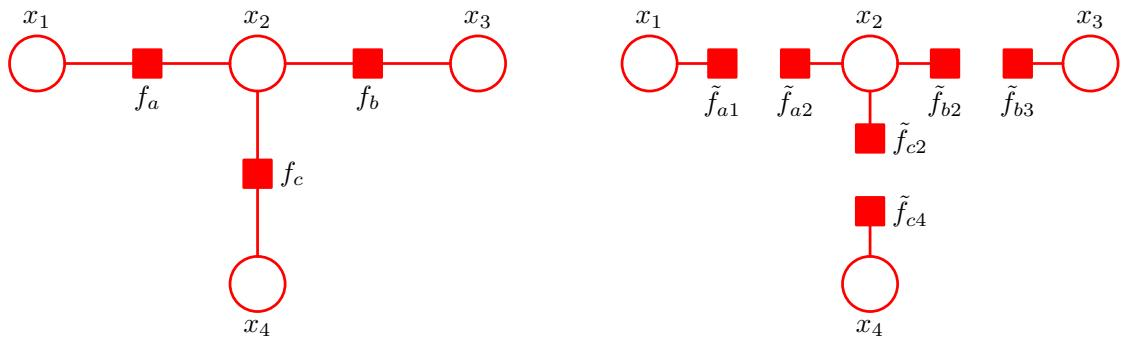
\includegraphics[keepaspectratio,alt={image}]{images/2f95516f719279751046c6e28592f07f4e06f8b76d00415fe88381c11a1c7730.jpg}}

Figure 10.18 On the left is a simple factor graph from Figure 8.51 and
reproduced here for convenience. On the right is the corresponding
factorized approximation.

\[
q ^ {\backslash b} (\mathbf {x}) = \widetilde {f} _ {a 1} (x _ {1}) \widetilde {f} _ {a 2} (x _ {2}) \widetilde {f} _ {c 2} (x _ {2}) \widetilde {f} _ {c 4} (x _ {4})\tag{10.228}
\]

and we then multiply this by the exact factor
\(f _ { b } ( x _ { 2 } , x _ { 3 } )\) to give

\[
\widehat {p} (\mathbf {x}) = q ^ {\backslash b} (\mathbf {x}) f _ {b} (x _ {2}, x _ {3}) = \widetilde {f} _ {a 1} (x _ {1}) \widetilde {f} _ {a 2} (x _ {2}) \widetilde {f} _ {c 2} (x _ {2}) \widetilde {f} _ {c 4} (x _ {4}) f _ {b} (x _ {2}, x _ {3}).\tag{10.229}
\]

We now find \(q ^ { \mathrm { n e w } } ( \mathbf { x } )\) by
minimizing the Kullback-Leibler divergence
\(\operatorname { K L } ( \widehat { p } \| q ^ { \mathrm { n e w } } )\)
The result, as noted above, is that
\(q ^ { \mathrm { n e w } } ( \mathbf { z } )\) comprises the product of
factors, one for each variable \(x _ { i }\) , in which each factor is
given by the corresponding marginal of \(\widehat { p } ( { \bf x } )\)
. These four marginals are given by

\[
\widehat {p} (x _ {1}) \propto \widetilde {f} _ {a 1} (x _ {1})\tag{10.230}
\]

\[
\widehat {p} (x _ {2}) \propto \widetilde {f} _ {a 2} (x _ {2}) \widetilde {f} _ {c 2} (x _ {2}) \sum_ {x _ {3}} f _ {b} (x _ {2}, x _ {3})\tag{10.231}
\]

\[
\widehat {p} (x _ {3}) \propto \sum_ {x _ {2}} \left\{f _ {b} (x _ {2}, x _ {3}) \widetilde {f} _ {a 2} (x _ {2}) \widetilde {f} _ {c 2} (x _ {2}) \right\}\tag{10.232}
\]

\[
\widehat {p} (x _ {4}) \propto \widetilde {f} _ {c 4} (x _ {4})\tag{10.233}
\]

and \(q ^ { \mathrm { n e w } } ( \mathbf { x } )\) is obtained by
multiplying these marginals together. We see that the only factors in
\(q ( \mathbf { x } )\) that change when we update
\(\widetilde { f } _ { b } ( x _ { 2 } , x _ { 3 } )\) are those that
involve the variables in \(f _ { b }\) namely \(x _ { 2 }\) and
\(x _ { 3 }\) . To obtain the refined factor
\(\widetilde { f } _ { b } ( x _ { 2 } , x _ { 3 } ) =\)
\(\widetilde { f } _ { b 2 } ( x _ { 2 } ) \widetilde { f } _ { b 3 } ( x _ { 3 } )\)
we simply divide \(q ^ { \mathrm { n e w } } ( \mathbf { x } )\) by
\(q ^ { \backslash b } ( { \mathbf { x } } )\) , which gives

\[
\widetilde {f} _ {b 2} (x _ {2}) \propto \sum_ {x _ {3}} f _ {b} (x _ {2}, x _ {3})\tag{10.234}
\]

\[
\widetilde {f} _ {b 3} (x _ {3}) \propto \sum_ {x _ {2}} \left\{f _ {b} (x _ {2}, x _ {3}) \widetilde {f} _ {a 2} (x _ {2}) \widetilde {f} _ {c 2} (x _ {2}) \right\}.\tag{10.235}
\]

These are precisely the messages obtained using belief propagation in
which messages from variable nodes to factor nodes have been folded into
the messages from factor nodes to variable nodes. In particular,
\(\widetilde { f } _ { b 2 } ( x _ { 2 } )\) corresponds to the message
\(\mu _ { f _ { b } \to x _ { 2 } } ( x _ { 2 } )\) sent by factor node
\(f _ { b }\) to variable node \(x _ { 2 }\) and is given by (8.81).
Similarly, if we substitute (8.78) into (8.79), we obtain (10.235) in
which \(\widetilde { f } _ { a 2 } ( x _ { 2 } )\) corresponds to
\(\mu _ { f _ { a } \to x _ { 2 } } ( x _ { 2 } )\) and
\(\widetilde { f } _ { c 2 } ( x _ { 2 } )\) corresponds to
\(\mu _ { f _ { c } \to x _ { 2 } } ( x _ { 2 } )\) , giving the message
\(\widetilde { f } _ { b 3 } ( x _ { 3 } )\) which corresponds to
\(\mu _ { f _ { b } \to x _ { 3 } } ( x _ { 3 } )\)

This result differs slightly from standard belief propagation in that
messages are passed in both directions at the same time. We can easily
modify the EP procedure to give the standard form of the sum-product
algorithm by updating just one of the factors at a time, for instance if
we refine only \(\widetilde { f } _ { b 3 } ( x _ { 3 } )\) , then
\(\widetilde { f } _ { b 2 } ( x _ { 2 } )\) is unchanged by definition,
while the refined version of
\(\widetilde { f } _ { b 3 } ( x _ { 3 } )\) is again given by (10.235).
If we are refining only one term at a time, then we can choose the order
in which the refinements are done as we wish. In particular, for a
tree-structured graph we can follow a two-pass update scheme,
corresponding to the standard belief propagation schedule, which will
result in exact inference of the variable and factor marginals. The
initialization of the approximation factors in this case is unimportant.

Now let us consider a general factor graph corresponding to the
distribution

\[
p (\boldsymbol {\theta}) = \prod_ {i} f _ {i} (\boldsymbol {\theta} _ {i})\tag{10.236}
\]

where \(\theta _ { i }\) represents the subset of variables associated
with factor \(f _ { i }\) . We approximate this using a fully factorized
distribution of the form

\[
q (\boldsymbol {\theta}) \propto \prod_ {i} \prod_ {k} \widetilde {f} _ {i k} (\theta_ {k})\tag{10.237}
\]

where \(\theta _ { k }\) corresponds to an individual variable node.
Suppose that we wish to refine the particular term
\(\widetilde { f } _ { j l } ( \theta _ { l } )\) keeping all other
terms fixed. We first remove the term
\(\widetilde { f } _ { j } ( \pmb { \theta } _ { j } )\) from
\(q ( \pmb \theta )\) to give

\[
q ^ {\backslash j} (\pmb {\theta}) \propto \prod_ {i \neq j} \prod_ {k} \widetilde {f} _ {i k} (\theta_ {k})\tag{10.238}
\]

and then multiply by the exact factor
\(f _ { j } ( \pmb { \theta } _ { j } )\) . To determine the refined
term \(\widetilde { f } _ { j l } ( \theta _ { l } )\) we need only
consider the functional dependence on \(\theta _ { l }\) , and so we
simply find the corresponding marginal of

\[
q ^ {\backslash j} (\boldsymbol {\theta}) f _ {j} \left(\boldsymbol {\theta} _ {j}\right).\tag{10.239}
\]

Up to a multiplicative constant, this involves taking the marginal of
\(f _ { j } ( \pmb { \theta } _ { j } )\) multiplied by any terms from
\(q ^ { \setminus j } ( \pmb \theta )\) that are functions of any of the
variables in \(\theta _ { j }\) . Terms that correspond to other factors
\(\widetilde { f } _ { i } ( \pmb \theta _ { i } )\) for \(i \neq j\)
will cancel between numerator and denominator when we subsequently
divide by \(q ^ { \setminus j } ( \pmb \theta )\) . We therefore obtain

\[
\widetilde {f} _ {j l} (\theta_ {l}) \propto \sum_ {\theta_ {m \neq l} \in \boldsymbol {\theta} _ {j}} f _ {j} (\boldsymbol {\theta} _ {j}) \prod_ {k} \prod_ {m \neq l} \widetilde {f} _ {k m} (\theta_ {m}).\tag{10.240}
\]

We recognize this as the sum-product rule in the form in which messages
from variable nodes to factor nodes have been eliminated, as illustrated
by the example shown in Figure 8.50. The quantity
\(\widetilde { f } _ { j m } ( \theta _ { m } )\) corresponds to the
message \(\mu _ { f _ { j } \to \theta _ { m } } ( \theta _ { m } )\)
which factor node \(j\) sends to variable node \(m ,\) and the product
over k in \(( 1 0 . 2 4 0 )\) is over all factors that depend on the
variables \(\theta _ { m }\) that have variables (other than variable
\(\theta _ { l } )\) in common with factor
\(f _ { j } ( \pmb { \theta } _ { j } )\) . In other words, to compute
the outgoing message from a factor node, we take the product of all the
incoming messages from other factor nodes, multiply by the local factor,
and then marginalize.

Thus, the sum-product algorithm arises as a special case of expectation
propagation if we use an approximating distribution that is fully
factorized. This suggests that more flexible approximating
distributions, corresponding to partially disconnected graphs, could be
used to achieve higher accuracy. Another generalization is to group
factors \(f _ { i } ( \pmb \theta _ { i } )\) together into sets and to
refine all the factors in a set together at each iteration. Both of
these approaches can lead to improvements in accuracy (Minka, 2001b). In
general, the problem of choosing the best combination of grouping and
disconnection is an open research issue.

We have seen that variational message passing and expectation
propagation optimize two different forms of the Kullback-Leibler
divergence. Minka (2005) has shown that a broad range of message passing
algorithms can be derived from a common framework involving minimization
of members of the alpha family of divergences, given by (10.19). These
include variational message passing, loopy belief propagation, and
expectation propagation, as well as a range of other algorithms, which
we do not have space to discuss here, such as tree-reweighted message
passing (Wainwright et al., 2005),fractional beliefpropagation
(Wiegerinck and Heskes, 2003), and power EP (Minka, 2004).

\subsection{Exercises}\label{exercises-2}

10.1 () www Verify that the log marginal distribution of the observed
data ln \(p ( \mathbf { X } )\) can be decomposed into two terms in the
form (10.2) where \(\mathcal { L } ( q )\) is given by (10.3) and
\(\mathrm { K L } ( q \| p )\) is given by (10.4).

10.2 () Use the properties \(\mathbb { E } [ z _ { 1 } ] = m _ { 1 }\)
and \(\mathbb { E } [ z _ { 2 } ] = m _ { 2 }\) to solve the
simultaneous equations (10.13) and (10.15), and hence show that,
provided the original distribution \(p ( \mathbf { z } )\) is
nonsingular, the unique solution for the means of the factors in the
approximation distribution is given by
\(\mathbb { E } [ z _ { 1 } ] = \mu _ { 1 }\) and
\(\mathbb { E } [ z _ { 2 } ] = \mu _ { 2 }\)

10.3 ( ) www Consider a factorized variational distribution
\(q ( \mathbf { Z } )\) of the form (10.5). By using the technique of
Lagrange multipliers, verify that minimization of the Kullback-Leibler
divergence \(\mathrm { K L } ( p \Vert q )\) with respect to one of the
factors \(q _ { i } ( \mathbf { Z } _ { i } )\) keeping all other
factors fixed, leads to the solution (10.17).

10.4 ( ) Suppose that \(p ( \mathbf { x } )\) is some fixed distribution
and that we wish to approximate it using a Gaussian distribution
\(q ( \mathbf { x } ) = \mathcal { N } ( \mathbf { x } | \boldsymbol { \mu } , \Sigma )\)
. By writing down the form of the KL divergence
\(\mathrm { K L } ( p | | q )\) for a Gaussian \(q ( \mathbf { x } )\)
and then differentiating, show that minimization of
\(\mathrm { K L } ( p | | q )\) with respect to \(\pmb { \mu }\) and
\(\pmb { \Sigma }\) leads to the result that \(\pmb { \mu }\) is given
by the expectation of x under \(p ( \mathbf { x } )\) and that Σ is
given by the covariance.

10.5 ( ) www Consider a model in which the set of all hidden stochastic
variables, denoted collectively by \(\mathbf { Z } ,\) comprises some
latent variables z together with some model parameters
\(\pmb { \theta } .\) Suppose we use a variational distribution that
factorizes between latent variables and parameters so that
\(q ( \mathbf { z } , \pmb { \theta } ) = q _ { \mathbf { z } } ( \mathbf { z } ) q _ { \pmb { \theta } } ( \pmb { \theta } )\)
, in which the distribution
\(q _ { \pmb { \theta } } ( \pmb { \theta } )\) is approximated by a
point estimate of the form
\({ q } _ { \pmb { \theta } } ( \pmb { \theta } ) = \delta ( \pmb { \theta } - \pmb { \theta } _ { 0 } )\)
where \(\theta _ { 0 }\) is a vector of free parameters. Show that
variational optimization of this factorized distribution is equivalent
to an EM algorithm, in which the E step optimizes
\(q _ { \mathbf { z } } ( \mathbf { z } )\) and the M step maximizes the
expected complete-data log posterior distribution of θ with respect to
\(\theta _ { 0 }\)

10.6 ( ) The alpha family of divergences is defined by (10.19). Show
that the Kullback-Leibler divergence \(\mathrm { K L } ( p \Vert q )\)
corresponds to \(\alpha  1\) . This can be done by writing
\(p ^ { \epsilon } = \exp ( \epsilon \ln p ) = 1 + \epsilon \ln p + O ( \epsilon ^ { 2 } )\)
and then taking \(\epsilon  0\) . Similarly show that
\(\mathrm { K L } ( q \| p )\) corresponds to \(\alpha  - 1\)

10.7 ( ) Consider the problem of inferring the mean and precision of a
univariate Gaussian using a factorized variational approximation, as
considered in Section 10.1.3. Show that the factor
\(q _ { \mu } ( \mu )\) is a Gaussian of the form
\(\mathcal { N } ( \mu \vert \mu _ { N } , \lambda _ { N } ^ { - 1 } )\)
with mean and precision given by (10.26) and (10.27), respectively.
Similarly show that the factor \(q _ { \tau } ( \tau )\) is a gamma
distribution of the form
\({ \mathrm { G a m } } ( \tau | a _ { N } , b _ { N } )\) with
parameters given by (10.29) and (10.30).

10.8 () Consider the variational posterior distribution for the
precision of a univariate Gaussian whose parameters are given by (10.29)
and (10.30). By using the standard results for the mean and variance of
the gamma distribution given by (B.27) and (B.28), show that if we let
\(N  \infty\) , this variational posterior distribution has a mean given
by the inverse of the maximum likelihood estimator for the variance of
the data, and a variance that goes to zero.

10.9 ( ) By making use of the standard result
\(\mathbb { E } [ \tau ] = a _ { N } / b _ { N }\) for the mean of a
gamma distribution, together with (10.26), (10.27), (10.29), and
(10.30), derive the result (10.33) for the reciprocal of the expected
precision in the factorized variational treatment of a univariate
Gaussian.

10.10 () www Derive the decomposition given by (10.34) that is used to
find approximate posterior distributions over models using variational
inference.

10.11 ( ) www By using a Lagrange multiplier to enforce the
normalization constraint on the distribution \(q ( m )\) , show that the
maximum of the lower bound (10.35) is given by (10.36).

10.12 ( ) Starting from the joint distribution (10.41), and applying the
general result (10.9), show that the optimal variational distribution
\(q ^ { \star } ( \mathbf { Z } )\) over the latent variables for the
Bayesian mixture of Gaussians is given by (10.48) by verifying the steps
given in the text.

10.13 ( ) www Starting from (10.54), derive the result (10.59) for the
optimum variational posterior distribution over \(\mu _ { k }\) and
\(\mathbf { \Lambda } _ { \Lambda _ { k } }\) in the Bayesian mixture of
Gaussians, and hence verify the expressions for the parameters of this
distribution given by (10.60)--(10.63).

10.14 ( ) Using the distribution (10.59), verify the result (10.64).

10.15 () Using the result (B.17), show that the expected value of the
mixing coefficients in the variational mixture of Gaussians is given by
(10.69).

10.16 ( ) www Verify the results (10.71) and (10.72) for the first two
terms in the lower bound for the variational Gaussian mixture model
given by (10.70).

10.17 (  ) Verify the results (10.73)--(10.77) for the remaining terms
in the lower bound for the variational Gaussian mixture model given by
(10.70).

10.18 (  ) In this exercise, we shall derive the variational
re-estimation equations for the Gaussian mixture model by direct
differentiation of the lower bound. To do this we assume that the
variational distribution has the factorization defined by (10.42) and
(10.55) with factors given by (10.48), (10.57), and (10.59). Substitute
these into (10.70) and hence obtain the lower bound as a function of the
parameters of the variational distribution. Then, by maximizing the
bound with respect to these parameters, derive the re-estimation
equations for the factors in the variational distribution, and show that
these are the same as those obtained in Section 10.2.1.

10.19 ( ) Derive the result (10.81) for the predictive distribution in
the variational treatment of the Bayesian mixture of Gaussians model.

10.20 ( ) www This exercise explores the variational Bayes solution for
the mixture of Gaussians model when the size N of the data set is large
and shows that it reduces (as we would expect) to the maximum likelihood
solution based on EM derived in Chapter 9. Note that results from
Appendix B may be used to help answer this exercise. First show that the
posterior distribution \(q ^ { \star } ( \Lambda _ { k } )\) of the
precisions becomes sharply peaked around the maximum likelihood
solution. Do the same for the posterior distribution of the means
\(q ^ { \star } ( \pmb { \mu } _ { k } | \pmb { \Lambda } _ { k } )\) .
Next consider the posterior distribution \(q ^ { \star } ( \pi )\) for
the mixing coefficients and show that this too becomes sharply peaked
around the maximum likelihood solution. Similarly, show that the
responsibilities become equal to the corresponding maximum likelihood
values for large N, by making use of the following asymptotic result for
the digamma function for large x

\[
\psi (x) = \ln x + O \left(1 / x\right).\tag{10.241}
\]

Finally, by making use of (10.80), show that for large N, the predictive
distribution becomes a mixture of Gaussians.

10.21 () Show that the number of equivalent parameter settings due to
interchange symmetries in a mixture model with K components is K!.

10.22 ( ) We have seen that each mode of the posterior distribution in a
Gaussian mixture model is a member of a family of K! equivalent modes.
Suppose that the result of running the variational inference algorithm
is an approximate posterior distribution \(q\) that is localized in the
neighbourhood of one of the modes. We can then approximate the full
posterior distribution as a mixture of \(K !\) such \(q\) distributions,
once centred on each mode and having equal mixing coefficients. Show
that if we assume negligible overlap between the components of the \(q\)
mixture, the resulting lower bound differs from that for a single
component \(q\) distribution through the addition of an extra term ln
\(K !\)

10.23 ( ) www Consider a variational Gaussian mixture model in which
there is no prior distribution over mixing coefficients
\(\{ \pi _ { k } \}\) . Instead, the mixing coefficients are treated as
parameters, whose values are to be found by maximizing the variational
lower bound on the log marginal likelihood. Show that maximizing this
lower bound with respect to the mixing coefficients, using a Lagrange
multiplier to enforce the constraint that the mixing coefficients sum to
one, leads to the re-estimation result (10.83). Note that there is no
need to consider all of the terms in the lower bound but only the
dependence of the bound on the \(\{ \pi _ { k } \}\)

10.24 ( ) www We have seen in Section 10.2 that the singularities
arising in the maximum likelihood treatment of Gaussian mixture models
do not arise in a Bayesian treatment. Discuss whether such singularities
would arise if the Bayesian model were solved using maximum posterior
(MAP) estimation.

10.25 ( ) The variational treatment of the Bayesian mixture of
Gaussians, discussed in Section 10.2, made use of a factorized
approximation (10.5) to the posterior distribution. As we saw in Figure
10.2, the factorized assumption causes the variance of the posterior
distribution to be under-estimated for certain directions in parameter
space. Discuss qualitatively the effect this will have on the
variational approximation to the model evidence, and how this effect
will vary with the number of components in the mixture. Hence explain
whether the variational Gaussian mixture will tend to under-estimate or
over-estimate the optimal number of components.

10.26 (  ) Extend the variational treatment of Bayesian linear
regression to include a gamma hyperprior Gam
\(( \beta | c _ { 0 } , d _ { 0 } )\) over \(\beta\) and solve
variationally, by assuming a factorized variational distribution of the
form \(q ( \mathbf { w } ) q ( \alpha ) q ( \beta )\) . Derive the
variational update equations for the three factors in the variational
distribution and also obtain an expression for the lower bound and for
the predictive distribution.

10.27 ( ) By making use of the formulae given in Appendix B show that
the variational lower bound for the linear basis function regression
model, defined by (10.107), can be written in the form (10.107) with the
various terms defined by (10.108)--(10.112).

10.28 (  ) Rewrite the model for the Bayesian mixture of Gaussians,
introduced in Section 10.2, as a conjugate model from the exponential
family, as discussed in Section 10.4. Hence use the general results
(10.115) and (10.119) to derive the specific results (10.48), (10.57),
and (10.59).

10.29 () www Show that the function \(f ( x ) = \ln ( x )\) is concave
for \(0 < x < \infty\) by computing its second derivative. Determine the
form of the dual function \(g ( \lambda )\) defined by (10.133), and
verify that minimization of \(\lambda x - g ( \lambda )\) with respect
to λ according to (10.132) indeed recovers the function ln(x).

10.30 () By evaluating the second derivative, show that the log logistic
function \(f ( x ) =\) \(- \ln ( 1 + e ^ { - x } )\) is concave. Derive
the variational upper bound (10.137) directly by making a second order
Taylor expansion of the log logistic function around a point \(x = \xi\)

10.31 ( ) By finding the second derivative with respect to x, show that
the function
\(f ( x ) = { \dot { - } } \ln ( e ^ { x { \mathord { \left/ { \vphantom { \mathrm { 1 2 } } } \right. \kern - delimiterspace } 2 } } + e ^ { - x / 2 } )\)
is a concave function of \(x .\) Now consider the second derivatives
with respect to the variable \(x ^ { 2 }\) and hence show that it is a
convex function of \(x ^ { 2 }\) . Plot graphs of \(f ( x )\) against x
and against \(x ^ { 2 }\) . Derive the lower bound (10.144) on the
logistic sigmoid function directly by making a first order Taylor series
expansion of the function \(f ( x )\) in the variable
\(x ^ { \mathrm { 2 } }\) centred on the value \(\xi ^ { 2 }\)

10.32 ( ) www Consider the variational treatment of logistic regression
with sequential learning in which data points are arriving one at a time
and each must be processed and discarded before the next data point
arrives. Show that a Gaussian approximation to the posterior
distribution can be maintained through the use of the lower bound
(10.151), in which the distribution is initialized using the prior, and
as each data point is absorbed its corresponding variational parameter
\(\xi _ { n }\) is optimized.

10.33 () By differentiating the quantity
\(Q ( \xi , \xi ^ { \mathrm { o l d } } )\) defined by (10.161) with
respect to the variational parameter \(\xi _ { n }\) show that the
update equation for \(\xi _ { n }\) for the Bayesian logistic regression
model is given by (10.163).

10.34 ( ) In this exercise we derive re-estimation equations for the
variational parameters \(\boldsymbol { \xi }\) in the Bayesian logistic
regression model of Section 4.5 by direct maximization of the lower
bound given by (10.164). To do this set the derivative of
\(\mathcal { L } ( \pmb { \xi } )\) with respect to \(\xi _ { n }\)
equal to zero, making use of the result (3.117) for the derivative of
the log of a determinant, together with the expressions (10.157) and
(10.158) which define the mean and covariance of the variational
posterior distribution \(q ( \mathbf { w } )\)

10.35 ( ) Derive the result (10.164) for the lower bound
\(\mathcal { L } ( \pmb { \xi } )\) in the variational logistic
regression model. This is most easily done by substituting the
expressions for the Gaussian prior
\(q ( \mathbf { w } ) = \mathcal { N } ( \mathbf { w } | \mathbf { m } _ { 0 } , \mathbf { S } _ { 0 } )\)
, together with the lower bound \(h ( \mathbf { w } , \pmb { \xi } )\)
on the likelihood function, into the integral (10.159) which defines
\(\mathcal { L } ( \pmb { \xi } )\) . Next gather together the terms
which depend on w in the exponential and complete the square to give a
Gaussian integral, which can then be evaluated by invoking the standard
result for the normalization coefficient of a multivariate Gaussian.
Finally take the logarithm to obtain (10.164).

10.36 ( ) Consider the ADF approximation scheme discussed in Section
10.7, and show that inclusion of the factor
\(f _ { j } ( \pmb \theta )\) leads to an update of the model evidence
of the form

\[
p _ {j} (\mathcal {D}) \simeq p _ {j - 1} (\mathcal {D}) Z _ {j}\tag{10.242}
\]

where \(Z _ { j }\) is the normalization constant defined by (10.197).
By applying this result recursively, and initializing with
\(p _ { 0 } ( \mathcal { D } ) = 1\) , derive the result

\[
p (\mathcal {D}) \simeq \prod_ {j} Z _ {j}.\tag{10.243}
\]

10.37 () www Consider the expectation propagation algorithm from Section
10.7, and suppose that one of the factors
\(f _ { 0 } ( \pmb { \theta } )\) in the definition (10.188) has the
same exponential family functional form as the approximating
distribution \(q ( \pmb \theta )\) . Show that if the factor
\(\widetilde { f } _ { 0 } ( \pmb { \theta } )\) is initialized to be
\(f _ { 0 } ( \pmb { \theta } )\) , then an EP update to refine
\(\widetilde { f } _ { 0 } ( \pmb { \theta } )\) leaves
\(\widetilde { f } _ { 0 } ( \pmb { \theta } )\)  unchanged. This
situation typically arises when one of the factors is the prior
\(p ( \pmb \theta )\) , and so we see that the prior factor can be
incorporated once exactly and does not need to be refined.

10.38 (  ) In this exercise and the next, we shall verify the results
(10.214)--(10.224) for the expectation propagation algorithm applied to
the clutter problem. Begin by using the division formula (10.205) to
derive the expressions (10.214) and (10.215) by completing the square
inside the exponential to identify the mean and variance. Also, show
that the normalization constant \(Z _ { n }\) , defined by (10.206), is
given for the clutter problem by (10.216). This can be done by making
use of the general result (2.115).

10.39 (  ) Show that the mean and variance of
\(q ^ { \mathrm { n e w } } ( \pmb { \theta } )\) for EP applied to the
clutter problem are given by (10.217) and (10.218). To do this, first
prove the following results for the expectations of \(\pmb \theta\) and
\(\boldsymbol { \theta \theta ^ { \mathrm { T } } }\) under
\(q ^ { \mathrm { n e w } } ( \pmb { \theta } )\)

\[
{\mathbb {E} [ \pmb {\theta} ]} = {\mathbf {m} ^ {\backslash n} + v ^ {\backslash n} \nabla_ {\mathbf {m} ^ {\backslash n}} \ln Z _ {n}}\tag{10.244}
\]

\[
\mathbb {E} [ \boldsymbol {\theta} ^ {\mathrm{T}} \boldsymbol {\theta} ] = 2 (v ^ {\backslash n}) ^ {2} \nabla_ {v ^ {\backslash n}} \ln Z _ {n} + 2 \mathbb {E} [ \boldsymbol {\theta} ] ^ {\mathrm{T}} \mathbf {m} ^ {\backslash n} - \| \mathbf {m} ^ {\backslash n} \| ^ {2}\tag{10.245}
\]

and then make use of the result (10.216) for \(Z _ { n }\) . Next, prove
the results (10.220)-- (10.222) by using (10.207) and completing the
square in the exponential. Finally, use (10.208) to derive the result
(10.223).

\subsection{11}\label{section}

\section{Sampling Methods}\label{sampling-methods}

\pandocbounded{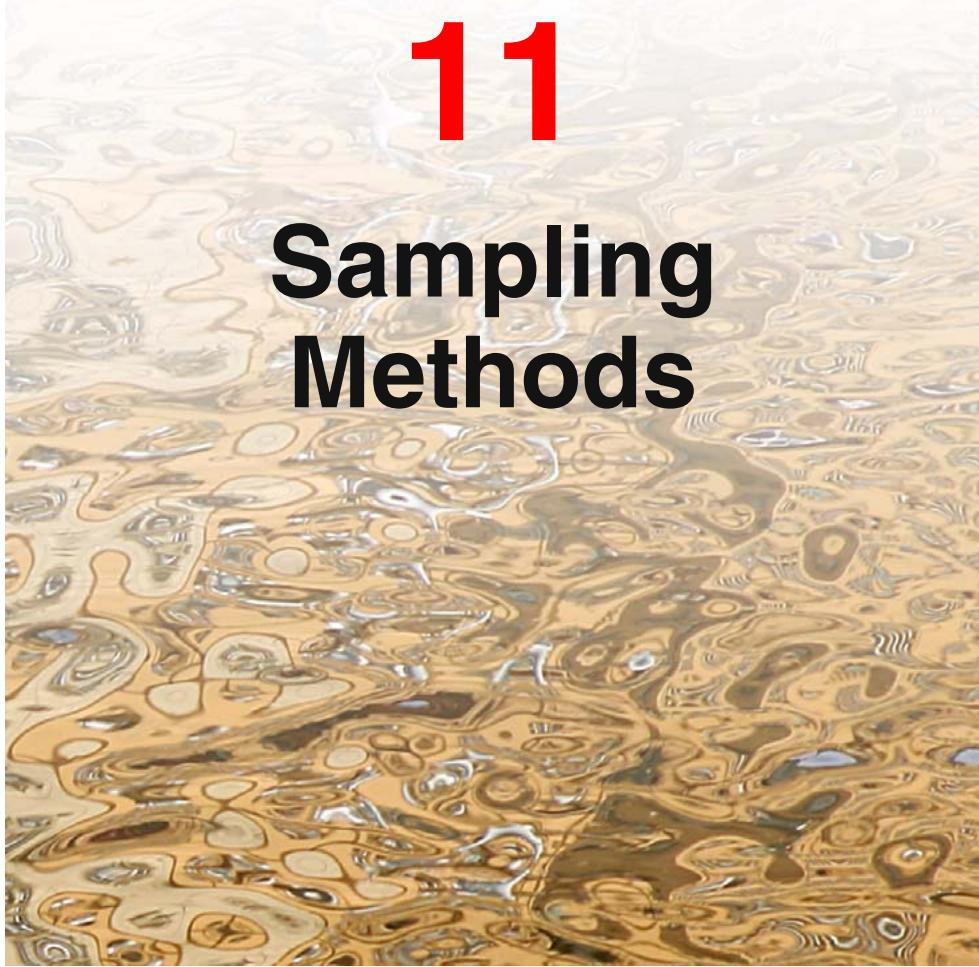
\includegraphics[keepaspectratio,alt={image}]{images/fb7eab15fe92dc6c124d411de3568c9b0c402dcc47eac69ffe1ac6f7fd4d8627.jpg}}

For most probabilistic models of practical interest, exact inference is
intractable, and so we have to resort to some form of approximation. In
Chapter 10, we discussed inference algorithms based on deterministic
approximations, which include methods such as variational Bayes and
expectation propagation. Here we consider approximate inference methods
based on numerical sampling, also known as Monte Carlo techniques.

Although for some applications the posterior distribution over
unobserved variables will be of direct interest in itself, for most
situations the posterior distribution is required primarily for the
purpose of evaluating expectations, for example in order to make
predictions. The fundamental problem that we therefore wish to address
in this chapter involves finding the expectation of some function f(z)
with respect to a probability distribution \(p ( \mathbf { z } )\) .
Here, the components of z might comprise discrete or continuous
variables or some combination of the two. Thus in the case of continuous

Figure 11.1 Schematic illustration of a function \(f ( z )\) whose
expectation is to be evaluated with respect to a distribution
\(p ( z )\)

\pandocbounded{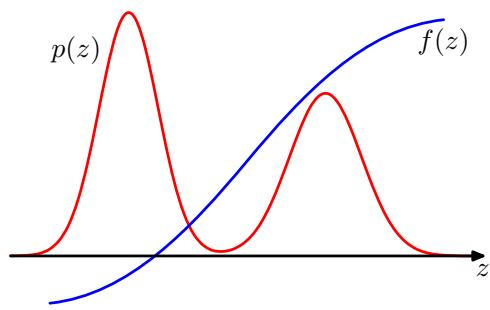
\includegraphics[keepaspectratio,alt={image}]{images/77626a0914ec748b7255d3e09957c40b347af937efbd691104c3b4913840d037.jpg}}

variables, we wish to evaluate the expectation

\[
\mathbb {E} [ f ] = \int f (\mathbf {z}) p (\mathbf {z}) \mathrm{d} \mathbf {z}\tag{11.1}
\]

where the integral is replaced by summation in the case of discrete
variables. This is illustrated schematically for a single continuous
variable in Figure 11.1. We shall suppose that such expectations are too
complex to be evaluated exactly using analytical techniques.

The general idea behind sampling methods is to obtain a set of samples
\(\mathbf { z } ^ { ( l ) }\) (where
\(l \stackrel { \cdot } { = } 1 , \ldots , L )\) drawn independently
from the distribution \(p ( \mathbf { z } )\) . This allows the
expectation (11.1) to be approximated by a finite sum

\[
\widehat {f} = \frac {1}{L} \sum_ {l = 1} ^ {L} f (\mathbf {z} ^ {(l)}).\tag{11.2}
\]

As long as the samples \(\mathbf { z } ^ { ( l ) }\) are drawn from the
distribution \(p ( \mathbf { z } )\) , then
\(\mathbb { E } [ \widehat { f } ] = \mathbb { E } [ f ]\) and so the
estimator \(\widehat { \boldsymbol { f } }\) has the correct mean. The
variance of the estimator is given by

\[
\operatorname{var} [ \widehat {f} ] = \frac {1}{L} \mathbb {E} \left[ (f - \mathbb {E} [ f ]) ^ {2} \right]\tag{11.3}
\]

is the variance of the function \(f ( \mathbf { z } )\) under the
distribution \(p ( \mathbf { z } )\) . It is worth emphasizing that the
accuracy of the estimator therefore does not depend on the
dimensionality of \(\mathbf { z } ,\) and that, in principle, high
accuracy may be achievable with a relatively small number of samples
\(\mathbf { z } ^ { ( l ) }\) . In practice, ten or twenty independent
samples may suffice to estimate an expectation to sufficient accuracy.

The problem, however, is that the samples
\(\{ \mathbf { z } ^ { ( l ) } \}\) might not be independent, and so the
effective sample size might be much smaller than the apparent sample
size. Also, referring back to Figure 11.1, we note that if
\(f ( \mathbf { z } )\) is small in regions where
\(p ( \mathbf { z } )\) is large, and vice versa, then the expectation
may be dominated by regions of small probability, implying that
relatively large sample sizes will be required to achieve sufficient
accuracy.

For many models, the joint distribution \(p ( \mathbf { z } )\) is
conveniently specified in terms of a graphical model. In the case of a
directed graph with no observed variables, it is straightforward to
sample from the joint distribution (assuming that it is possible to
sample from the conditional distributions at each node) using the
following ancestral sampling approach, discussed briefly in Section
8.1.2. The joint distribution is specified by

\[
p (\mathbf {z}) = \prod_ {i = 1} ^ {M} p (\mathbf {z} _ {i} | \mathrm{pa} _ {i})\tag{11.4}
\]

where \(\mathbf { z } _ { i }\) are the set of variables associated with
node \(i ,\) and \(\mathrm { p a } _ { i }\) denotes the set of
variables associated with the parents of node i. To obtain a sample from
the joint distribution, we make one pass through the set of variables in
the order \(\mathbf { z } _ { 1 } , \ldots , \mathbf { z } _ { M }\)
sampling from the conditional distributions
\(p ( \mathbf { z } _ { i } | \mathrm { p a } _ { i } )\) . This is
always possible because at each step all of the parent values will have
been instantiated. After one pass through the graph, we will have
obtained a sample from the joint distribution.

Now consider the case of a directed graph in which some of the nodes are
instantiated with observed values. We can in principle extend the above
procedure, at least in the case of nodes representing discrete
variables, to give the following logic sampling approach (Henrion,
1988), which can be seen as a special case of importance sampling
discussed in Section 11.1.4. At each step, when a sampled value is
obtained for a variable \(\mathbf { z } _ { i }\) whose value is
observed, the sampled value is compared to the observed value, and if
they agree then the sample value is retained and the algorithm proceeds
to the next variable in turn. However, if the sampled value and the
observed value disagree, then the whole sample so far is discarded and
the algorithm starts again with the first node in the graph. This
algorithm samples correctly from the posterior distribution because it
corresponds simply to drawing samples from the joint distribution of
hidden variables and data variables and then discarding those samples
that disagree with the observed data (with the slight saving of not
continuing with the sampling from the joint distribution as soon as one
contradictory value is observed). However, the overall probability of
accepting a sample from the posterior decreases rapidly as the number of
observed variables increases and as the number of states that those
variables can take increases, and so this approach is rarely used in
practice.

In the case of probability distributions defined by an undirected graph,
there is no one-pass sampling strategy that will sample even from the
prior distribution with no observed variables. Instead, computationally
more expensive techniques must be employed, such as Gibbs sampling,
which is discussed in Section 11.3.

As well as sampling from conditional distributions, we may also require
samples from a marginal distribution. If we already have a strategy for
sampling from a joint distribution
\(p ( \mathbf { u } , \mathbf { v } )\) , then it is straightforward to
obtain samples from the marginal distribution \(p ( \mathbf { u } )\)
simply by ignoring the values for v in each sample.

There are numerous texts dealing with Monte Carlo methods. Those of
particular interest from the statistical inference perspective include
Chen et al.~(2001), Gamerman (1997), Gilks et al.~(1996), Liu (2001),
Neal (1996), and Robert and Casella (1999). Also there are review
articles by Besag et al.~(1995), Brooks (1998), Diaconis and
Saloff-Coste (1998), Jerrum and Sinclair (1996), Neal (1993), Tierney
(1994), and Andrieu et al.~(2003) that provide additional information on
sampling

methods for statistical inference.

Diagnostic tests for convergence of Markov chain Monte Carlo algorithms
are summarized in Robert and Casella (1999), and some practical guidance
on the use of sampling methods in the context of machine learning is
given in Bishop and Nabney (2008).

\subsection{11.1. Basic Sampling
Algorithms}\label{basic-sampling-algorithms}

In this section, we consider some simple strategies for generating
random samples from a given distribution. Because the samples will be
generated by a computer algorithm they will in fact be pseudo-random
numbers, that is, they will be deterministically calculated, but must
nevertheless pass appropriate tests for randomness. Generating such
numbers raises several subtleties (Press et \(a l .\) , 1992) that lie
outside the scope of this book. Here we shall assume that an algorithm
has been provided that generates pseudo-random numbers distributed
uniformly over \(( 0 , 1 )\) , and indeed most software environments
have such a facility built in.

\subsection{11.1.1 Standard distributions}\label{standard-distributions}

We first consider how to generate random numbers from simple nonuniform
distributions, assuming that we already have available a source of
uniformly distributed random numbers. Suppose that z is uniformly
distributed over the interval \(( 0 , 1 )\) and that we transform the
values of z using some function \(f ( \cdot )\) so that \(y = f ( z )\)
The distribution of \(y\) will be governed by

\[
p (y) = p (z) \left| \frac {d z}{d y} \right|\tag{11.5}
\]

where, in this case, \(p ( z ) = 1\) . Our goal is to choose the
function \(f ( z )\) such that the resulting values of \(y\) have some
specific desired distribution \(p ( y )\) . Integrating (11.5) we obtain

\[
z = h (y) \equiv \int_ {- \infty} ^ {y} p (\widehat {y}) \mathrm{d} \widehat {y}\tag{11.6}
\]

which is the indefinite integral of \(p ( y )\) . Thus,
\(y = h ^ { - 1 } ( z )\) , and so we have to transform the uniformly
distributed random numbers using a function which is the inverse of the
indefinite integral of the desired distribution. This is illustrated in
Figure 11.2.

Consider for example the exponential distribution

\[
p (y) = \lambda \exp (- \lambda y)\tag{11.7}
\]

where \(0 \leqslant y < \infty\) . In this case the lower limit of the
integral in (11.6) is 0, and so \(h ( y ) = 1 - \exp ( - \lambda y )\) .
Thus, if we transform our uniformly distributed variable \(z\) using
\(y = - \lambda ^ { - 1 } \ln ( 1 - z )\) , then \(y\) will have an
exponential distribution.

Figure 11.2 Geometrical interpretation of the transformation method for
generating nonuniformly distributed random numbers. \(h ( y )\) is the
indefinite integral of the desired distribution \(p ( y )\) If a
uniformly distributed random variable z is transformed using
\(y = h ^ { - 1 } ( z )\) , then y will be distributed according to
\(p ( y )\)

\pandocbounded{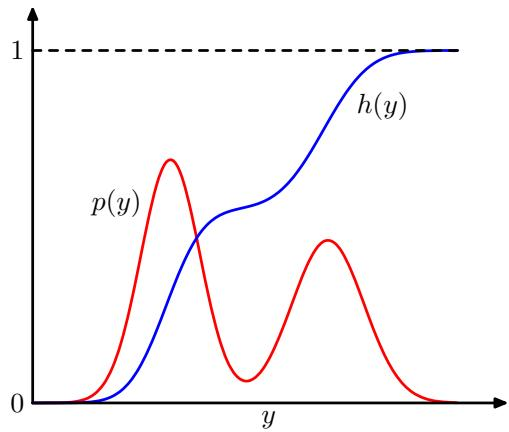
\includegraphics[keepaspectratio,alt={image}]{images/c59ac6ad7e0b8a93288b26effbf69cf1b2292eedc7fe0f1d08050469031bb4a9.jpg}}

Another example of a distribution to which the transformation method can
be applied is given by the Cauchy distribution

\[
p (y) = \frac {1}{\pi} \frac {1}{1 + y ^ {2}}.\tag{11.8}
\]

In this case, the inverse of the indefinite integral can be expressed in
terms of the `tan' function.

The generalization to multiple variables is straightforward and involves
the Jacobian of the change of variables, so that

\[
p (y _ {1}, \dots , y _ {M}) = p (z _ {1}, \dots , z _ {M}) \left| \frac {\partial (z _ {1} , \dots , z _ {M})}{\partial (y _ {1} , \dots , y _ {M})} \right|.\tag{11.9}
\]

As a final example of the transformation method we consider the
Box-Muller method for generating samples from a Gaussian distribution.
First, suppose we generate pairs of uniformly distributed random numbers
\(z _ { 1 } , z _ { 2 } \in ( - 1 , 1 )\) , which we can do by
transforming a variable distributed uniformly over (0, 1) using
\(z  2 z - 1\) Next we discard each pair unless it satisfies
\(z _ { 1 } ^ { 2 } + \dot { z } _ { 2 } ^ { 2 } \leqslant 1\) This
leads to a uniform distribution of points inside the unit circle with
\(p ( z _ { 1 } , z _ { 2 } ) = 1 / \pi\) , as illustrated in Figure
11.3. Then, for each pair \(z _ { 1 } , z _ { 2 }\) we evaluate the
quantities

Figure 11.3 The Box-Muller method for generating Gaussian distributed
random numbers starts by generating samples from a uniform distribution
inside the unit circle.

\pandocbounded{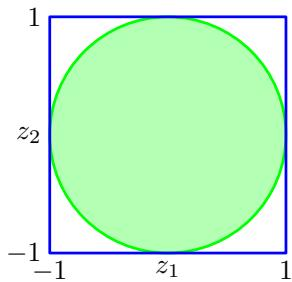
\includegraphics[keepaspectratio,alt={image}]{images/cc71f140b5f19c6bf8666cabd597f5d60e2480257b5b8a87d232063560352012.jpg}}

\[
y _ {1} = z _ {1} \left(\frac {- 2 \ln z _ {1}}{r ^ {2}}\right) ^ {1 / 2}\tag{11.10}
\]

\[
{y _ {2}} = {z _ {2} \left(\frac {- 2 \ln z _ {2}}{r ^ {2}}\right) ^ {1 / 2}}\tag{11.11}
\]

where \(r ^ { 2 } = z _ { 1 } ^ { 2 } + z _ { 2 } ^ { 2 }\) . Then the
joint distribution of \(y _ { 1 }\) and \(y _ { 2 }\) is given by

\[
\begin{array}{r c l} p (y _ {1}, y _ {2}) & = & p (z _ {1}, z _ {2}) \left| \frac {\partial (z _ {1} , z _ {2})}{\partial (y _ {1} , y _ {2})} \right| \\ & = & \left[ \frac {1}{\sqrt {2 \pi}} \exp (- y _ {1} ^ {2} / 2) \right] \left[ \frac {1}{\sqrt {2 \pi}} \exp (- y _ {2} ^ {2} / 2) \right] \end{array}\tag{11.12}
\]

and so \(y _ { 1 }\) and \(y _ { 2 }\) are independent and each has a
Gaussian distribution with zero mean and unit variance.

If \(y\) has a Gaussian distribution with zero mean and unit variance,
then \(\sigma y + \mu\) will have a Gaussian distribution with mean
\(\mu\) and variance \(\sigma ^ { 2 }\) . To generate vectorvalued
variables having a multivariate Gaussian distribution with mean
\(\pmb { \mu }\) and covariance Σ, we can make use of the Cholesky
decomposition, which takes the form
\({ \pmb \Sigma } = { \bf L L } ^ { \mathrm { T } }\) (Press et al.,
1992). Then, if z is a vector valued random variable whose components
are independent and Gaussian distributed with zero mean and unit
variance, then \(\mathbf { y } = \pmb { \mu } + \mathbf { L z }\) will
have mean \(\pmb { \mu }\) and covariance Σ.

Obviously, the transformation technique depends for its success on the
ability to calculate and then invert the indefinite integral of the
required distribution. Such operations will only be feasible for a
limited number of simple distributions, and so we must turn to
alternative approaches in search of a more general strategy. Here we
consider two techniques called rejection sampling and importance
sampling. Although mainly limited to univariate distributions and thus
not directly applicable to complex problems in many dimensions, they do
form important components in more general strategies.

\subsection{11.1.2 Rejection sampling}\label{rejection-sampling}

The rejection sampling framework allows us to sample from relatively
complex distributions, subject to certain constraints. We begin by
considering univariate distributions and discuss the extension to
multiple dimensions subsequently.

Suppose we wish to sample from a distribution \(p ( \mathbf { z } )\)
that is not one of the simple, standard distributions considered so far,
and that sampling directly from \(p ( \mathbf { z } )\) is difficult.
Furthermore suppose, as is often the case, that we are easily able to
evaluate \(p ( \mathbf { z } )\) for any given value of
\(\mathbf { z } ,\) up to some normalizing constant \(Z .\) , so that

\[
p (z) = \frac {1}{Z _ {p}} \widetilde {p} (z)\tag{11.13}
\]

where \(\widetilde { p } ( z )\) can readily be evaluated, but
\(Z _ { p }\) is unknown.

In order to apply rejection sampling, we need some simpler distribution
\(q ( z )\) sometimes called a proposal distribution, from which we can
readily draw samples.

Figure 11.4 In the rejection sampling method, samples are drawn from a
simple distribution \(q ( z )\) and rejected if they fall in the grey
area between the unnormalized distribution \(\widetilde { p } ( z )\)
and the scaled distribution \(k q ( z )\) . The resulting samples are
distributed according to \(p ( z )\) which is the normalized version of
\(\widetilde { p } ( z )\)

\pandocbounded{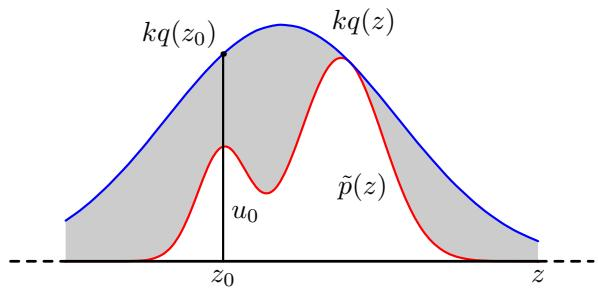
\includegraphics[keepaspectratio,alt={image}]{images/13b768754d7209253ed73330dcd16e2febaf33884a377f6467ab8edfe3dc06de.jpg}}

We next introduce a constant k whose value is chosen such that
\(k q ( z ) \geqslant \widetilde { p } ( z )\) for all values of z. The
function \(k q ( z )\) is called the comparison function and is
illustrated for a univariate distribution in Figure 11.4. Each step of
the rejection sampler involves generating two random numbers. First, we
generate a number \(z _ { \mathrm { 0 } }\) from the distribution
\(q ( z )\) . Next, we generate a number \(u _ { 0 }\) from the uniform
distribution over \([ 0 , k q ( z _ { 0 } ) ]\) . This pair of random
numbers has uniform distribution under the curve of the function
\(k q ( z )\) . Finally, if
\(u _ { 0 } > \widetilde { p } ( z _ { 0 } )\) then the sample is
rejected, otherwise \(u _ { 0 }\) is retained. Thus the pair is rejected
if it lies in the grey shaded region in Figure 11.4. The remaining pairs
then have uniform distribution under the curve of
\(\widetilde { p } ( z )\) and hence the corresponding z values are
distributed according to \(p ( z )\) , as desired.

The original values of z are generated from the distribution \(q ( z )\)
, and these samples are then accepted with probability
\(\widetilde { p } ( z ) / k q ( z )\) , and so the probability that a
sample will be accepted is given by

\[
\begin{array}{r c l} {p (\mathrm{accept})} & = & {\int \{\widetilde {p} (z) / k q (z) \} q (z) \mathrm{d} z} \\ & = & {\frac {1}{k} \int \widetilde {p} (z) \mathrm{d} z.} \end{array}\tag{11.14}
\]

Thus the fraction of points that are rejected by this method depends on
the ratio of the area under the unnormalized distribution
\(\tilde { p } ( z )\) to the area under the curve \(k q ( z )\) We
therefore see that the constant k should be as small as possible subject
to the limitation that \(k q ( z )\) must be nowhere less than
\(\widetilde { p } ( z )\)

As an illustration of the use of rejection sampling, consider the task
of sampling from the gamma distribution

\[
\operatorname{Gam} (z | a, b) = \frac {b ^ {a} z ^ {a - 1} \exp (- b z)}{\Gamma (a)}\tag{11.15}
\]

which, for \(a \ > \ 1\) , has a bell-shaped form, as shown in Figure
11.5. A suitable proposal distribution is therefore the Cauchy (11.8)
because this too is bell-shaped and because we can use the
transformation method, discussed earlier, to sample from it. We need to
generalize the Cauchy slightly to ensure that it nowhere has a smaller
value than the gamma distribution. This can be achieved by transforming
a uniform random variable y using \(z = b \tan y + c ,\) which gives
random numbers distributed according to.

Plot showing the gamma distribution given by (11.15) as the green curve,
with a scaled Cauchy proposal distribution shown by the red curve.
Samples from the gamma distribution can be obtained by sampling from the
Cauchy and then applying the rejection sampling criterion.

Exercise 11.9

\pandocbounded{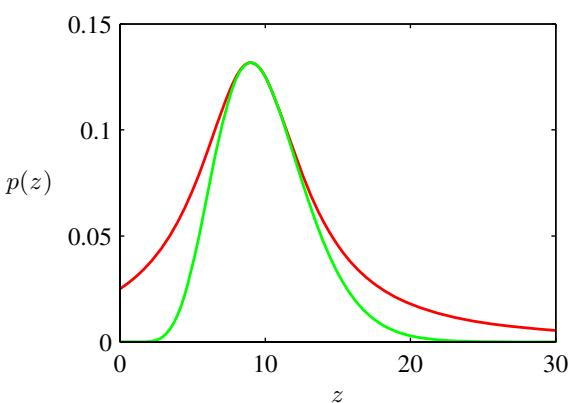
\includegraphics[keepaspectratio,alt={image}]{images/9f63f1761610a413fcb0636168c9ffa6f036358a66e29f168f5a6f317bd2557c.jpg}}

\[
q (z) = \frac {k}{1 + (z - c) ^ {2} / b ^ {2}}.\tag{11.16}
\]

The minimum reject rate is obtained by setting
\(c = a - 1 , b ^ { 2 } = 2 a - 1\) and choosing the constant k to be as
small as possible while still satisfying the requirement
\(k q ( z ) \geqslant \widetilde { p } ( z )\) . The resulting
comparison function is also illustrated in Figure 11.5.

\subsection{11.1.3 Adaptive rejection
sampling}\label{adaptive-rejection-sampling}

In many instances where we might wish to apply rejection sampling, it
proves difficult to determine a suitable analytic form for the envelope
distribution \(q ( z )\) . An alternative approach is to construct the
envelope function on the fly based on measured values of the
distribution \(p ( z )\) (Gilks and Wild, 1992). Construction of an
envelope function is particularly straightforward for cases in which
\(p ( z )\) is log concave, in other words when ln \(p ( z )\) has
derivatives that are nonincreasing functions of z. The construction of a
suitable envelope function is illustrated graphically in Figure 11.6.

The function ln \(p ( z )\) and its gradient are evaluated at some
initial set of grid points, and the intersections of the resulting
tangent lines are used to construct the envelope function. Next a sample
value is drawn from the envelope distribution. This is straightforward
because the log of the envelope distribution is a succession of linear
functions, and hence the envelope distribution itself comprises a
piecewise exponential distribution of the form

In the case of distributions that are log concave, an envelope function
for use in rejection sampling can be constructed using the tangent lines
computed at a set of grid points. If a sample point is rejected, it is
added to the set of grid points and used to refine the envelope
distribution.

\pandocbounded{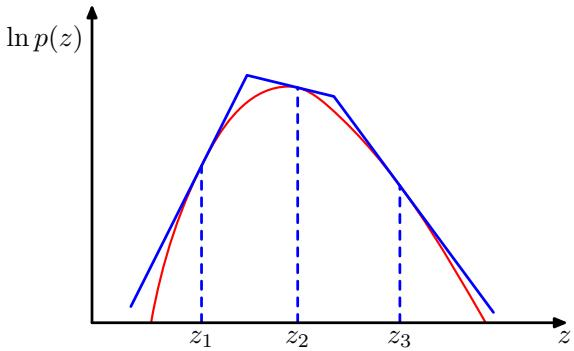
\includegraphics[keepaspectratio,alt={image}]{images/38b36c30d57b20e7fc55c772d3d035cac44464dcf656455fe2482ef6e28609d6.jpg}}

Figure 11.7 Illustrative example of rejection sampling involving
sampling from a Gaussian distribution \(p ( z )\) shown by the green
curve, by using rejection sampling from a proposal distribution
\(\overset { \cdot } { q } ( z )\) that is also Gaussian and whose
scaled version \(k q ( z )\) is shown by the red curve.

\pandocbounded{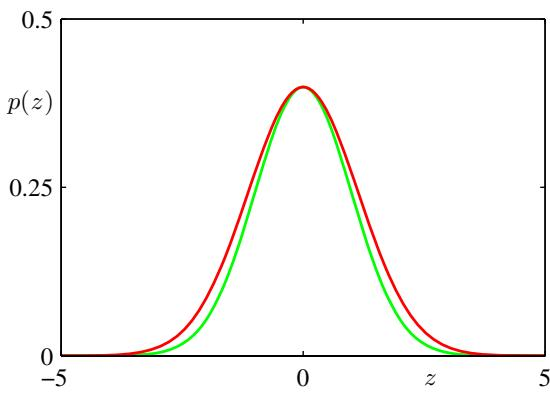
\includegraphics[keepaspectratio,alt={image}]{images/51c28c7dda4af343ce0b04ed09053123b117ecfaf63b28e9bca13b05d0f31f0b.jpg}}

\[
q (z) = k _ {i} \lambda_ {i} \exp \left\{- \lambda_ {i} (z - z _ {i - 1}) \right\} \quad z _ {i - 1} <   z \leqslant z _ {i}.\tag{11.17}
\]

Once a sample has been drawn, the usual rejection criterion can be
applied. If the sample is accepted, then it will be a draw from the
desired distribution. If, however, the sample is rejected, then it is
incorporated into the set of grid points, a new tangent line is
computed, and the envelope function is thereby refined. As the number of
grid points increases, so the envelope function becomes a better
approximation of the desired distribution \(p ( z )\) and the
probability of rejection decreases.

A variant of the algorithm exists that avoids the evaluation of
derivatives (Gilks, 1992). The adaptive rejection sampling framework can
also be extended to distributions that are not log concave, simply by
following each rejection sampling step with a Metropolis-Hastings step
(to be discussed in Section 11.2.2), giving rise to adaptive rejection
Metropolis sampling (Gilks et al., 1995).

Clearly for rejection sampling to be of practical value, we require that
the comparison function be close to the required distribution so that
the rate of rejection is kept to a minimum. Now let us examine what
happens when we try to use rejection sampling in spaces of high
dimensionality. Consider, for the sake of illustration, a somewhat
artificial problem in which we wish to sample from a zero-mean
multivariate Gaussian distribution with covariance
\(\sigma _ { p } ^ { 2 } \mathbf { I }\) , where I is the unit matrix,
by rejection sampling from a proposal distribution that is itself a
zero-mean Gaussian distribution having covariance
\({ \bar { \sigma } } _ { q } ^ { 2 } \mathbf { I }\) . Obviously, we
must have \(\sigma _ { q } ^ { 2 } \geqslant \sigma _ { p } ^ { 2 }\) in
order that there exists a k such that
\(k q ( z ) \stackrel { \triangledown } { \geqslant } p ( z )\) . In
D-dimensions the optimum value of k is given by
\(k = ( \sigma _ { q } / \sigma _ { p } ) ^ { D }\) , as illustrated for
\(D = 1\) in Figure 11.7. The acceptance rate will be the ratio of
volumes under \(p ( z )\) and \(k q ( z )\) , which, because both
distributions are normalized, is just \(1 / k\) . Thus the acceptance
rate diminishes exponentially with dimensionality. Even if
\(\sigma _ { q }\) exceeds \(\sigma _ { p }\) by just one percent, for
\(D = 1 , 0 0 0\) the acceptance ratio will be approximately
\(1 / 2 0 , 0 0 0\) In this illustrative example the comparison function
is close to the required distribution. For more practical examples,
where the desired distribution may be multimodal and sharply peaked, it
will be extremely difficult to find a good proposal distribution and
comparison function.

Figure 11.8 Importance sampling addresses the problem of evaluating the
expectation of a function \(f ( z )\) with respect to a distribution
\(p ( z )\) from which it is difficult to draw samples directly.
Instead, samples \(\{ z ^ { ( l ) } \}\) are drawn from a simpler
distribution \(q ( z )\) , and the corresponding terms in the summation
are weighted by the ratios \(p ( z ^ { ( l ) } ) / q ( z ^ { ( l ) } )\)
.

\pandocbounded{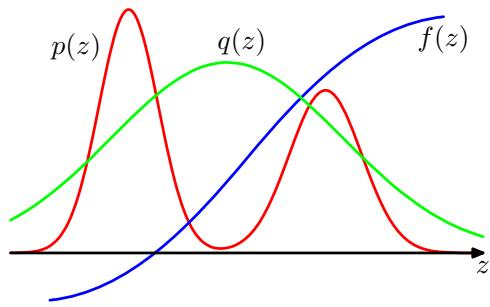
\includegraphics[keepaspectratio,alt={image}]{images/f5f8ead216940804d29fb060c83e03fb3ecb9d18d2fed30683cde1abba04deb6.jpg}}

Furthermore, the exponential decrease of acceptance rate with
dimensionality is a generic feature of rejection sampling. Although
rejection can be a useful technique in one or two dimensions it is
unsuited to problems of high dimensionality. It can, however, play a
role as a subroutine in more sophisticated algorithms for sampling in
high dimensional spaces.

\subsection{11.1.4 Importance sampling}\label{importance-sampling}

One of the principal reasons for wishing to sample from complicated
probability distributions is to be able to evaluate expectations of the
form (11.1). The technique of importance sampling provides a framework
for approximating expectations directly but does not itself provide a
mechanism for drawing samples from distribution \(p ( \mathbf { z } )\)

The finite sum approximation to the expectation, given by (11.2),
depends on being able to draw samples from the distribution
\(p ( \mathbf { z } )\) . Suppose, however, that it is impractical to
sample directly from \(p ( \mathbf { z } )\) but that we can evaluate
\(p ( \mathbf { z } )\) easily for any given value of
\(\mathbf { z } .\) One simplistic strategy for evaluating expectations
would be to discretize z-space into a uniform grid and to evaluate the
integrand as a sum of the form

\[
\mathbb {E} [ f ] \simeq \sum_ {l = 1} ^ {L} p (\mathbf {z} ^ {(l)}) f (\mathbf {z} ^ {(l)}).\tag{11.18}
\]

An obvious problem with this approach is that the number of terms in the
summation grows exponentially with the dimensionality of
\(\mathbf { z } .\) . Furthermore, as we have already noted, the kinds
of probability distributions of interest will often have much of their
mass confined to relatively small regions of z space and so uniform
sampling will be very inefficient because in high-dimensional problems,
only a very small proportion of the samples will make a significant
contribution to the sum. We would really like to choose the sample
points to fall in regions where \(p ( \mathbf { z } )\) is large, or
ideally where the product \(p ( \mathbf { z } ) f ( \mathbf { z } )\) is
large.

As in the case of rejection sampling, importance sampling is based on
the use of a proposal distribution \(q ( \mathbf { z } )\) from which it
is easy to draw samples, as illustrated in Figure 11.8. We can then
express the expectation in the form of a finite sum over

samples \(\{ \mathbf { z } ^ { ( l ) } \}\) drawn from
\(q ( \mathbf { z } )\)

\[
\begin{array}{r c l} \mathbb {E} [ f ] & = & \int f (\mathbf {z}) p (\mathbf {z})   \mathrm{d} \mathbf {z} \\ & = & \int f (\mathbf {z}) \frac {p (\mathbf {z})}{q (\mathbf {z})} q (\mathbf {z})   \mathrm{d} \mathbf {z} \\ & \simeq & \frac {1}{L} \sum_ {l = 1} ^ {L} \frac {p (\mathbf {z} ^ {(l)})}{q (\mathbf {z} ^ {(l)})} f (\mathbf {z} ^ {(l)}). \end{array}\tag{11.19}
\]

The quantities
\(r _ { l } = p ( \mathbf { z } ^ { ( l ) } ) / q ( \mathbf { z } ^ { ( l ) } )\)
are known as importance weights, and they correct the bias introduced by
sampling from the wrong distribution. Note that, unlike rejection
sampling, all of the samples generated are retained.

It will often be the case that the distribution \(p ( \mathbf { z } )\)
can only be evaluated up to a normalization constant, so that
\(p ( \mathbf { z } ) = \widetilde { p } ( \mathbf { z } ) / Z _ { p }\)
where \(\widetilde { p } ( \mathbf { z } )\) can be evaluated easily,
whereas \(Z _ { p }\)  is unknown. Similarly, we may wish to use an
importance sampling distribution
\(q ( \mathbf { z } ) = \widetilde { q } ( \mathbf { z } ) / Z _ { q }\)
, which has the same property. We then have

\[
\begin{array}{r c l} \mathbb {E} [ f ] & = & \int f (\mathbf {z}) p (\mathbf {z}) \mathrm{d} \mathbf {z} \\ & = & \frac {Z _ {q}}{Z _ {p}} \int f (\mathbf {z}) \frac {\widetilde {p} (\mathbf {z})}{\widetilde {q} (\mathbf {z})} q (\mathbf {z}) \mathrm{d} \mathbf {z} \\ & \simeq & \frac {Z _ {q}}{Z _ {p}} \frac {1}{L} \sum_ {l = 1} ^ {L} \widetilde {r} _ {l} f (\mathbf {z} ^ {(l)}). \end{array}\tag{11.20}
\]

where
\(\widetilde { r } _ { l } = \widetilde { p } ( \mathbf { z } ^ { ( l ) } ) / \widetilde { q } ( \mathbf { z } ^ { ( l ) } )\)
. We can use the same sample set to evaluate the ratio
\(Z _ { p } / Z _ { q }\) with the result

\[
\begin{array}{r c l} \frac {Z _ {p}}{Z _ {q}} & = & \frac {1}{Z _ {q}} \int \widetilde {p} (\mathbf {z}) \mathrm{d} \mathbf {z} = \int \frac {\widetilde {p} (\mathbf {z})}{\widetilde {q} (\mathbf {z})} q (\mathbf {z}) \mathrm{d} \mathbf {z} \\ & \simeq & \frac {1}{L} \sum_ {l = 1} ^ {L} \widetilde {r _ {l}} \end{array}\tag{11.21}
\]

and hence

\[
\mathbb {E} [ f ] \simeq \sum_ {l = 1} ^ {L} w _ {l} f (\mathbf {z} ^ {(l)})\tag{11.22}
\]

where we have defined

\[
w _ {l} = \frac {\widetilde {r} _ {l}}{\sum_ {m} \widetilde {r} _ {m}} = \frac {\widetilde {p} (\mathbf {z} ^ {(l)}) / q (\mathbf {z} ^ {(l)})}{\sum_ {m} \widetilde {p} (\mathbf {z} ^ {(m)}) / q (\mathbf {z} ^ {(m)})}.\tag{11.23}
\]

As with rejection sampling, the success of the importance sampling
approach depends crucially on how well the sampling distribution
\(q ( \mathbf { z } )\) matches the desired distribution
\(p ( \mathbf { z } )\) . If, as is often the case,
\(p ( \mathbf { z } ) f ( \mathbf { z } )\) is strongly varying and has
a sig nificant proportion of its mass concentrated over relatively small
regions of z space, then the set of importance weights
\(\{ r _ { l } \}\) may be dominated by a few weights having large
values, with the remaining weights being relatively insignificant. Thus
the effective sample size can be much smaller than the apparent sample
size \(L .\) . The problem is even more severe if none of the samples
falls in the regions where \(p ( \mathbf { z } ) f ( \mathbf { z } )\)
is large. In that case, the apparent variances of \(r _ { l }\) and
\(r _ { l } f ( \mathbf { z } ^ { ( \overline { { l } } ) } )\) may be
small even though the estimate of the expectation may be severely wrong.
Hence a major drawback of the importance sampling method is the
potential to produce results that are arbitrarily in error and with no
diagnostic indication. This also highlights a key requirement for the
sampling distribution \(q ( \mathbf { z } )\) , namely that it should
not be small or zero in regions where \(p ( \mathbf { z } )\) may be
significant.

For distributions defined in terms of a graphical model, we can apply
the importance sampling technique in various ways. For discrete
variables, a simple approach is called uniform sampling. The joint
distribution for a directed graph is defined by (11.4). Each sample from
the joint distribution is obtained by first setting those variables
\(\mathbf { z } _ { i }\) that are in the evidence set equal to their
observed values. Each of the remaining variables is then sampled
independently from a uniform distribution over the space of possible
instantiations. To determine the corresponding weight associated with a
sample \(\mathbf { z } ^ { ( l ) }\) , we note that the sampling
distribution \(\widetilde { \boldsymbol { q } } ( \mathbf { z } )\) is
uniform over the possible choices for \(\mathbf { z } ,\) and that
\(\widetilde { p } ( \mathbf { z } | \mathbf { x } ) = \widetilde { p } ( \mathbf { z } )\)
, where x denotes the subset of variables that are observed, and the
equality follows from the fact that every sample z that is generated is
necessarily consistent with the evidence. Thus the weights \(r _ { l }\)
are simply proportional to \(p ( \mathbf { z } )\) . Note that the
variables can be sampled in any order. This approach can yield poor
results if the posterior distribution is far from uniform, as is often
the case in practice.

An improvement on this approach is called likelihood weighted sampling
(Fung and Chang, 1990; Shachter and Peot, 1990) and is based on
ancestral sampling of the variables. For each variable in turn, if that
variable is in the evidence set, then it is just set to its instantiated
value. If it is not in the evidence set, then it is sampled from the
conditional distribution
\(p ( \mathbf { z } _ { i } | \mathrm { p a } _ { i } )\) in which the
conditioning variables are set to their currently sampled values. The
weighting associated with the resulting sample z is then given by

\[
r (\mathbf {z}) = \prod_ {\mathbf {z} _ {i} \not \in \mathbf {e}} \frac {p (\mathbf {z} _ {i} | \mathrm{pa} _ {i})}{p (\mathbf {z} _ {i} | \mathrm{pa} _ {i})} \prod_ {\mathbf {z} _ {i} \in \mathbf {e}} \frac {p (\mathbf {z} _ {i} | \mathrm{pa} _ {i})}{1} = \prod_ {\mathbf {z} _ {i} \in \mathbf {e}} p (\mathbf {z} _ {i} | \mathrm{pa} _ {i}).\tag{11.24}
\]

This method can be further extended using self-importance sampling
(Shachter and Peot, 1990) in which the importance sampling distribution
is continually updated to reflect the current estimated posterior
distribution.

\subsection{11.1.5
Sampling-importance-resampling}\label{sampling-importance-resampling}

The rejection sampling method discussed in Section 11.1.2 depends in
part for its success on the determination of a suitable value for the
constant k. For many pairs of distributions \(p ( \mathbf { z } )\) and
\(q ( \mathbf { z } )\) , it will be impractical to determine a suitable
value for k in that any value that is sufficiently large to guarantee a
bound on the desired distribution will lead to impractically small
acceptance rates.

As in the case of rejection sampling, the sampling-importance-resampling
(SIR) approach also makes use of a sampling distribution
\(q ( \mathbf { z } )\) but avoids having to determine the constant k.
There are two stages to the scheme. In the first stage, \(L\) samples
\(\mathbf { z } ^ { ( 1 ) } , \ldots , \mathbf { z } ^ { ( L ) }\) are
drawn from \(q ( \mathbf { z } )\) . Then in the second stage, weights
\(w _ { 1 } , \ldots , w _ { L }\) are constructed using (11.23).
Finally, a second set of \(L\) samples is drawn from the discrete
distribution
\(( \mathbf { z } ^ { ( 1 ) } , \ldots , \mathbf { z } ^ { ( L ) } )\)
with probabilities given by the weights
\(( w _ { 1 } , \dots , w _ { L } )\)

The resulting L samples are only approximately distributed according to
\(p ( \mathbf { z } )\) but the distribution becomes correct in the
limit \(L  \infty\) . To see this, consider the univariate case, and
note that the cumulative distribution of the resampled values is given
by

\[
\begin{array}{r c l} p (z \leqslant a) & = & \sum_ {l: z ^ {(l)} \leqslant a} w _ {l} \\ & = & \frac {\sum_ {l} I (z ^ {(l)} \leqslant a) \widetilde {p} (z ^ {(l)}) / q (z ^ {(l)})}{\sum_ {l} \widetilde {p} (z ^ {(l)}) / q (z ^ {(l)})} \end{array}\tag{11.25}
\]

where \(I ( . )\) is the indicator function (which equals 1 if its
argument is true and 0 otherwise). Taking the limit \(L  \infty\) , and
assuming suitable regularity of the distributions, we can replace the
sums by integrals weighted according to the original sampling
distribution \(q ( z )\)

\[
\begin{array}{l l l} p (z \leqslant a) & = & \frac { \int I (z \leqslant a)   \{\widetilde {p} (z) / q (z) \}   q (z)   \mathrm{d} z}{ \int \{\widetilde {p} (z) / q (z) \}   q (z)   \mathrm{d} z} \\ & = & \frac { \int I (z \leqslant a) \widetilde {p} (z)   \mathrm{d} z}{ \int \widetilde {p} (z)   \mathrm{d} z} \\ & = & \int I (z \leqslant a) p (z)   \mathrm{d} z \end{array}\tag{11.26}
\]

which is the cumulative distribution function of \(p ( z )\) . Again, we
see that the normalization of \(p ( z )\) is not required.

For a finite value of \(L ,\) and a given initial sample set, the
resampled values will only approximately be drawn from the desired
distribution. As with rejection sampling, the approximation improves as
the sampling distribution \(q ( \mathbf { z } )\) gets closer to the
desired distribution \(p ( \mathbf { z } )\) . When
\(q ( \mathbf { z } ) = p ( \mathbf { z } )\) , the initial samples
\(( \mathbf { z } ^ { ( 1 ) } , \ldots , \mathbf { z } ^ { ( L ) } )\)
have the desired distribution, and the weights \(w _ { n } = 1 / L\) so
that the resampled values also have the desired distribution.

If moments with respect to the distribution \(p ( \mathbf { z } )\) are
required, then they can be

evaluated directly using the original samples together with the weights,
because

\[
\begin{array}{r c l} \mathbb {E} [ f (\mathbf {z}) ] & = & \int f (\mathbf {z}) p (\mathbf {z})   \mathrm{d} \mathbf {z} \\ & = & \frac {\int f (\mathbf {z}) [ \widetilde {p} (\mathbf {z}) / q (\mathbf {z}) ] q (\mathbf {z})   \mathrm{d} \mathbf {z}}{\int [ \widetilde {p} (\mathbf {z}) / q (\mathbf {z}) ] q (\mathbf {z})   \mathrm{d} \mathbf {z}} \\ & \simeq & \sum_ {l = 1} ^ {L} w _ {l} f (\mathbf {z} _ {l}). \end{array}\tag{11.27}
\]

\subsection{11.1.6 Sampling and the EM
algorithm}\label{sampling-and-the-em-algorithm}

In addition to providing a mechanism for direct implementation of the
Bayesian framework, Monte Carlo methods can also play a role in the
frequentist paradigm, for example to find maximum likelihood solutions.
In particular, sampling methods can be used to approximate the E step of
the EM algorithm for models in which the E step cannot be performed
analytically. Consider a model with hidden variables Z, visible
(observed) variables \(\mathbf { X } ,\) , and parameters
\(\pmb { \theta } .\) . The function that is optimized with respect to
\(\pmb \theta\) in the M step is the expected complete-data log
likelihood, given by

\[
Q (\pmb {\theta}, \pmb {\theta} ^ {\mathrm{old}}) = \int p (\mathbf {Z} | \mathbf {X}, \pmb {\theta} ^ {\mathrm{old}}) \ln p (\mathbf {Z}, \mathbf {X} | \pmb {\theta}) \mathrm{d} \mathbf {Z}.\tag{11.28}
\]

We can use sampling methods to approximate this integral by a finite sum
over samples \(\{ \mathbf { Z } ^ { ( l ) } \}\) , which are drawn from
the current estimate for the posterior distribution
\(p ( { \bf Z } | { \bf X } , \boldsymbol { \theta } ^ { \mathrm { o l d } } )\)
, so that

\[
Q (\boldsymbol {\theta}, \boldsymbol {\theta} ^ {\mathrm{old}}) \simeq \frac {1}{L} \sum_ {l = 1} ^ {L} \ln p (\mathbf {Z} ^ {(l)}, \mathbf {X} | \boldsymbol {\theta}).\tag{11.29}
\]

The \(Q\) function is then optimized in the usual way in the M step.
This procedure is called the Monte Carlo EM algorithm.

It is straightforward to extend this to the problem of finding the mode
of the posterior distribution over \(\pmb \theta\) (the MAP estimate)
when a prior distribution \(p ( \pmb \theta )\) has been defined, simply
by adding ln \(p ( \pmb \theta )\) to the function
\(Q ( \theta , \theta ^ { \mathrm { o l d } } )\) before performing the
M step.

A particular instance of the Monte Carlo EM algorithm, called stochastic
EM, arises if we consider a finite mixture model, and draw just one
sample at each E step. Here the latent variable Z characterizes which of
the K components of the mixture is responsible for generating each data
point. In the E step, a sample of Z is taken from the posterior
distribution
\(p ( { \bf Z } | { \bf X } , \boldsymbol { \theta } ^ { \mathrm { { \bar { o l d } } } } )\)
where X is the data set. This effectively makes a hard assignment of
each data point to one of the components in the mixture. In the M step,
this sampled approximation to the posterior distribution is used to
update the model parameters in the usual way.

Now suppose we move from a maximum likelihood approach to a full
Bayesian treatment in which we wish to sample from the posterior
distribution over the parameter vector θ. In principle, we would like to
draw samples from the joint posterior
\(p ( \pmb { \theta } , \mathbf { Z } | \mathbf { X } )\) , but we shall
suppose that this is computationally difficult. Suppose further that it
is relatively straightforward to sample from the complete-data parameter
posterior \(p ( \pmb { \theta } | \mathbf { Z } , \mathbf { X } )\) .
This inspires the data augmentation algorithm, which alternates between
two steps known as the I-step (imputation step, analogous to an E step)
and the P-step (posterior step, analogous to an M step).

\subsection{IP Algorithm}\label{ip-algorithm}

I-step. We wish to sample from \(p ( \mathbf { Z } | \mathbf { X } )\)
but we cannot do this directly. We therefore note the relation

\[
p (\mathbf {Z} | \mathbf {X}) = \int p (\mathbf {Z} | \boldsymbol {\theta}, \mathbf {X}) p (\boldsymbol {\theta} | \mathbf {X}) \mathrm{d} \boldsymbol {\theta}\tag{11.30}
\]

and hence for \(l = 1 , \ldots , L\) we first draw a sample
\(\pmb \theta ^ { ( l ) }\) from the current estimate for
\(p ( \pmb \theta | \mathbf X )\) , and then use this to draw a sample
\(\mathbf { Z } ^ { ( l ) }\) from
\(p ( \mathbf { Z } | \pmb { \theta } ^ { ( l ) } , \mathbf { X } )\) .
P-step. Given the relation

\[
p (\pmb {\theta} | \mathbf {X}) = \int p (\pmb {\theta} | \mathbf {Z}, \mathbf {X}) p (\mathbf {Z} | \mathbf {X}) \mathrm{d} \mathbf {Z}\tag{11.31}
\]

we use the samples \(\{ \mathbf { Z } ^ { ( l ) } \}\) obtained from the
I-step to compute a revised estimate of the posterior distribution over
θ given by

\[
p (\boldsymbol {\theta} | \mathbf {X}) \simeq \frac {1}{L} \sum_ {l = 1} ^ {L} p (\boldsymbol {\theta} | \mathbf {Z} ^ {(l)}, \mathbf {X}).\tag{11.32}
\]

By assumption, it will be feasible to sample from this approximation in
the I-step.

Note that we are making a (somewhat artificial) distinction between
parameters θ and hidden variables Z. From now on, we blur this
distinction and focus simply on the problem of drawing samples from a
given posterior distribution.

\subsection{11.2. Markov Chain Monte
Carlo}\label{markov-chain-monte-carlo}

In the previous section, we discussed the rejection sampling and
importance sampling strategies for evaluating expectations of functions,
and we saw that they suffer from severe limitations particularly in
spaces of high dimensionality. We therefore turn in this section to a
very general and powerful framework called Markov chain Monte Carlo
(MCMC), which allows sampling from a large class of distributions, and
which scales well with the dimensionality of the sample space. Markov
chain Monte Carlo methods have their origins in physics (Metropolis and
Ulam, 1949), and it was only towards the end of the 1980s that they
started to have a significant impact in the field of statistics.

As with rejection and importance sampling, we again sample from a
proposal distribution. This time, however, we maintain a record of the
current state \(\bar { \mathbf { z } } ^ { ( \tau ) }\) , and the
proposal distribution
\(q ( \mathbf { z } | \mathbf { z } ^ { ( \tau ) } )\) ) depends on this
current state, and so the sequence of samples
\({ \bf z } ^ { ( 1 ) } , { \bf z } ^ { ( 2 ) } , . . .\) . forms a
Markov chain. Again, if we write
\(p ( \mathbf { z } ) = \widetilde { p } ( \mathbf { \bar { z } } ) / Z _ { p }\)
we will assume that \(\widetilde { p } ( \mathbf { z } )\) can readily
be evaluated for any given value of \(\mathbf { z } ,\) , although the
value of \(Z _ { p }\) may be unknown. The proposal distribution itself
is chosen to be sufficiently simple that it is straightforward to draw
samples from it directly. At each cycle of the algorithm, we generate a
candidate sample \(\mathbf { z } ^ { \star }\) from the proposal
distribution and then accept the sample according to an appropriate
criterion.

In the basic Metropolis algorithm (Metropolis et al., 1953), we assume
that the proposal distribution is symmetric, that is
\(q ( \mathbf { z } _ { A } | \mathbf { z } _ { B } ) = q ( \mathbf { z } _ { B } | \mathbf { z } _ { A } )\)
for all values of \(\mathbf { z } _ { A }\) and
\(\mathbf { z } _ { B }\) . The candidate sample is then accepted with
probability

\[
A (\mathbf {z} ^ {\star}, \mathbf {z} ^ {(\tau)}) = \min \left(1, \frac {\widetilde {p} (\mathbf {z} ^ {\star})}{\widetilde {p} (\mathbf {z} ^ {(\tau)})}\right).\tag{11.33}
\]

This can be achieved by choosing a random number u with uniform
distribution over the unit interval \(( 0 , 1 )\) and then accepting the
sample if
\(A ( \mathbf { z } ^ { \star } , \mathbf { z } ^ { ( \tau ) } ) > u\) .
Note that if the step from \(\mathbf { z } ^ { ( \tau ) }\) to
\(\mathbf { z } ^ { \star }\) causes an increase in the value of
\(p ( \mathbf { z } )\) , then the candidate point is certain to be
kept.

If the candidate sample is accepted, then
\(\mathbf { z } ^ { ( \tau + 1 ) } = \mathbf { z } ^ { \star }\) ,
otherwise the candidate point \(\mathbf { z } ^ { \star }\) is
discarded, \(\mathbf { z } ^ { ( \hat { \tau } + 1 ) }\) is set to
\(\mathbf { z } ^ { ( \tau ) }\) and another candidate sample is drawn
from the distribution
\({ \boldsymbol { q } } ( \mathbf { z } | \mathbf { z } ^ { ( \tau + 1 ) } )\)
. This is in contrast to rejection sampling, where rejected samples are
simply discarded. In the Metropolis algorithm when a candidate point is
rejected, the previous sample is included instead in the final list of
samples, leading to multiple copies of samples. Of course, in a
practical implementation, only a single copy of each retained sample
would be kept, along with an integer weighting factor recording how many
times that state appears. As we shall see, as long as
\(q ( { \bf z } _ { A } | { \bf z } _ { B } )\) is positive for any
values of \(\mathbf { z } _ { A }\) and \(\mathbf { z } _ { B }\) (this
is a sufficient but not necessary condition), the distribution of
\(\mathbf { z } ^ { ( \tau ) }\) tends to \(p ( \mathbf { z } )\) as
\(\tau \to \infty\) . It should be emphasized, however, that the
sequence \({ \bf z } ^ { ( 1 ) } , { \bf z } ^ { ( 2 ) } , . . .\) . is
not a set of independent samples from \(p ( \mathbf { z } )\) because
successive samples are highly correlated. If we wish to obtain
independent samples, then we can discard most of the sequence and just
retain every \(\hat { M } ^ { \mathrm { t h } }\) sample. For M
sufficiently large, the retained samples will for all practical purposes
be independent. Figure 11.9 shows a simple illustrative example of
sampling from a two-dimensional Gaussian distribution using the
Metropolis algorithm in which the proposal distribution is an isotropic
Gaussian.

Further insight into the nature of Markov chain Monte Carlo algorithms
can be gleaned by looking at the properties of a specific example,
namely a simple random

A simple illustration using Metropolis algorithm to sample from a
Gaussian distribution whose one standard-deviation contour is shown by
the ellipse. The proposal distribution is an isotropic Gaussian
distribution whose standard deviation is 0.2. Steps that are accepted
are shown as green lines, and rejected steps are shown in red. A total
of 150 candidate samples are generated, of which 43 are rejected.

\pandocbounded{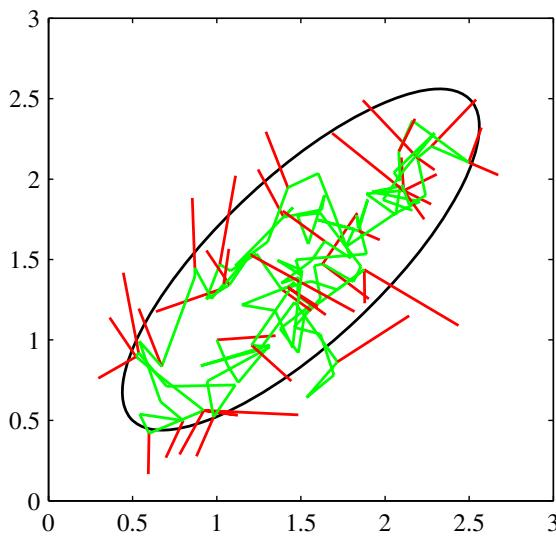
\includegraphics[keepaspectratio,alt={image}]{images/be575be2ca005f2fb8de6d7f9c9eb903d8a7cdac70682b3735e5b55e1a462524.jpg}}

walk. Consider a state space z consisting of the integers, with
probabilities

\[
p (z ^ {(\tau + 1)} = z ^ {(\tau)}) = 0. 5\tag{11.34}
\]

\[
p (z ^ {(\tau + 1)} = z ^ {(\tau)} + 1) = 0. 2 5\tag{11.35}
\]

\[
p (z ^ {(\tau + 1)} = z ^ {(\tau)} - 1) = 0. 2 5\tag{11.36}
\]

Exercise 11.10

where \(z ^ { ( \tau ) }\) denotes the state at step τ. If the initial
state is \(z ^ { ( 1 ) } = 0\) , then by symmetry the expected state at
time \(\tau\) will also be zero
\(\mathbb { E } [ z ^ { ( \tau ) } ] = 0\) , and similarly it is easily
seen that E
\(\bar { \iota } [ ( z ^ { ( \tau ) } ) ^ { 2 } ] = \tau / 2\) . Thus
after τ steps, the random walk has only travelled a distance that on
average is proportional to the square root of \(\tau\) . This square
root dependence is typical of random walk behaviour and shows that
random walks are very inefficient in exploring the state space. As we
shall see, a central goal in designing Markov chain Monte Carlo methods
is to avoid random walk behaviour.

\subsection{11.2.1 Markov chains}\label{markov-chains}

Before discussing Markov chain Monte Carlo methods in more detail, it is
useful to study some general properties of Markov chains in more detail.
In particular, we ask under what circumstances will a Markov chain
converge to the desired distribution. A first-order Markov chain is
defined to be a series of random variables
\(\mathbf { z } ^ { ( 1 ) } , \ldots , \mathbf { z } ^ { ( M ) }\) such
that the following conditional independence property holds for
\(m \in \{ 1 , \ldots , M - 1 \}\)

\[
p (\mathbf {z} ^ {(m + 1)} | \mathbf {z} ^ {(1)}, \dots , \mathbf {z} ^ {(m)}) = p (\mathbf {z} ^ {(m + 1)} | \mathbf {z} ^ {(m)}).\tag{11.37}
\]

This of course can be represented as a directed graph in the form of a
chain, an example of which is shown in Figure 8.38. We can then specify
the Markov chain by giving the probability distribution for the initial
variable \(p ( \mathbf { z } ^ { ( 0 ) } )\) ) together with the
conditional probabilities for subsequent variables in the form of
transition probabilities
\(T _ { m } ( \mathbf { z } ^ { ( \hat { m } ) } , \mathbf { z } ^ { ( m + 1 ) } ) \equiv p ( \mathbf { z } ^ { ( m + 1 ) } | \mathbf { z } ^ { ( m ) } )\)
. A Markov chain is called homogeneous if the transition probabilities
are the same for all m.

The marginal probability for a particular variable can be expressed in
terms of the marginal probability for the previous variable in the chain
in the form

\[
p (\mathbf {z} ^ {(m + 1)}) = \sum_ {\mathbf {z} ^ {(m)}} p (\mathbf {z} ^ {(m + 1)} | \mathbf {z} ^ {(m)}) p (\mathbf {z} ^ {(m)}).\tag{11.38}
\]

A distribution is said to be invariant, or stationary, with respect to a
Markov chain if each step in the chain leaves that distribution
invariant. Thus, for a homogeneous Markov chain with transition
probabilities \(T ( \mathbf { z } ^ { \prime } , \mathbf { z } )\) , the
distribution \(p ^ { \star } ( \mathbf { z } )\) is invariant if

\[
p ^ {\star} (\mathbf {z}) = \sum_ {\mathbf {z} ^ {\prime}} T (\mathbf {z} ^ {\prime}, \mathbf {z}) p ^ {\star} (\mathbf {z} ^ {\prime}).\tag{11.39}
\]

Note that a given Markov chain may have more than one invariant
distribution. For instance, if the transition probabilities are given by
the identity transformation, then any distribution will be invariant.

A sufficient (but not necessary) condition for ensuring that the
required distribution \(p ( \mathbf { z } )\) is invariant is to choose
the transition probabilities to satisfy the property of detailed
balance, defined by

\[
p ^ {\star} (\mathbf {z}) T (\mathbf {z}, \mathbf {z} ^ {\prime}) = p ^ {\star} (\mathbf {z} ^ {\prime}) T (\mathbf {z} ^ {\prime}, \mathbf {z})\tag{11.40}
\]

for the particular distribution \(p ^ { \star } ( \mathbf { z } )\) . It
is easily seen that a transition probability that satisfies detailed
balance with respect to a particular distribution will leave that
distribution invariant, because

\[
\sum_ {\mathbf {z} ^ {\prime}} p ^ {\star} (\mathbf {z} ^ {\prime}) T (\mathbf {z} ^ {\prime}, \mathbf {z}) = \sum_ {\mathbf {z} ^ {\prime}} p ^ {\star} (\mathbf {z}) T (\mathbf {z}, \mathbf {z} ^ {\prime}) = p ^ {\star} (\mathbf {z}) \sum_ {\mathbf {z} ^ {\prime}} p (\mathbf {z} ^ {\prime} | \mathbf {z}) = p ^ {\star} (\mathbf {z}).\tag{11.41}
\]

A Markov chain that respects detailed balance is said to be reversible.

Our goal is to use Markov chains to sample from a given distribution. We
can achieve this if we set up a Markov chain such that the desired
distribution is invariant. However, we must also require that for
\(m \to \infty\) , the distribution \(p ( \mathbf { z } ^ { ( m ) } )\)
) converges to the required invariant distribution
\(p ^ { \star } ( \mathbf { z } )\) , irrespective of the choice of
initial distribution
\({ \bf \bar { \rho } } _ { p } ( { \bf z } ^ { ( 0 ) } )\) . This
property is called ergodicity, and the invariant distribution is then
called the equilibrium distribution. Clearly, an ergodic Markov chain
can have only one equilibrium distribution. It can be shown that a
homogeneous Markov chain will be ergodic, subject only to weak
restrictions on the invariant distribution and the transition
probabilities (Neal, 1993).

In practice we often construct the transition probabilities from a set
of `base transitions \(B _ { 1 } , \ldots , B _ { K }\) . This can be
achieved through a mixture distribution of the form

\[
T (\mathbf {z} ^ {\prime}, \mathbf {z}) = \sum_ {k = 1} ^ {K} \alpha_ {k} B _ {k} (\mathbf {z} ^ {\prime}, \mathbf {z})\tag{11.42}
\]

for some set of mixing coefficients
\(\alpha _ { 1 } , \ldots , \alpha _ { K }\) satisfying
\(\alpha _ { k } \geqslant 0\) and
\(\textstyle \sum _ { k } \alpha _ { k } = 1\) Alternatively, the base
transitions may be combined through successive application, so that

\[
T (\mathbf {z} ^ {\prime}, \mathbf {z}) = \sum_ {\mathbf {z} _ {1}} \dots \sum_ {\mathbf {z} _ {n - 1}} B _ {1} (\mathbf {z} ^ {\prime}, \mathbf {z} _ {1}) \dots B _ {K - 1} (\mathbf {z} _ {K - 2}, \mathbf {z} _ {K - 1}) B _ {K} (\mathbf {z} _ {K - 1}, \mathbf {z}).\tag{11.43}
\]

If a distribution is invariant with respect to each of the base
transitions, then obviously it will also be invariant with respect to
either of the \(T ( \mathbf { z } ^ { \prime } , \mathbf { z } )\) given
by (11.42) or (11.43). For the case of the mixture (11.42), if each of
the base transitions satisfies detailed balance, then the mixture
transition \(T\) will also satisfy detailed balance. This does not hold
for the transition probability constructed using (11.43), although by
symmetrizing the order of application of the base transitions, in the
form
\(B _ { 1 } , B _ { 2 } , \ldots , B _ { K } , B _ { K } , \ldots , B _ { 2 } , B _ { 1 }\)
, detailed balance can be restored. A common example of the use of
composite transition probabilities is where each base transition changes
only a subset of the variables.

\subsection{11.2.2 The Metropolis-Hastings
algorithm}\label{the-metropolis-hastings-algorithm}

Earlier we introduced the basic Metropolis algorithm, without actually
demonstrating that it samples from the required distribution. Before
giving a proof, we first discuss a generalization, known as the
Metropolis-Hastings algorithm (Hastings, 1970), to the case where the
proposal distribution is no longer a symmetric function of its
arguments. In particular at step τ of the algorithm, in which the
current state is \(\mathbf { z } ^ { ( \tau ) }\) , we draw a sample
\(\mathbf { z } ^ { \star }\) from the distribution
\(q _ { k } ( \mathbf { z } | \mathbf { z } ^ { ( \tau ) } )\) and then
accept it with probability
\(A _ { k } ( { \bf z } ^ { \star } , { \bf z } _ { \tau } )\) where

\[
A _ {k} (\mathbf {z} ^ {\star}, \mathbf {z} ^ {(\tau)}) = \min \left(1, \frac {\widetilde {p} (\mathbf {z} ^ {\star}) q _ {k} (\mathbf {z} ^ {(\tau)} | \mathbf {z} ^ {\star})}{\widetilde {p} (\mathbf {z} ^ {(\tau)}) q _ {k} (\mathbf {z} ^ {\star} | \mathbf {z} ^ {(\tau)})}\right).\tag{11.44}
\]

Here k labels the members of the set of possible transitions being
considered. Again, the evaluation of the acceptance criterion does not
require knowledge of the normalizing constant \(Z _ { p }\) in the
probability distribution
\(p ( \mathbf { z } ) \bar { \mathbf { \rho } } = \widetilde { p } ( \mathbf { z } ) / Z _ { p }\)
. For a symmetric proposal distribution the Metropolis-Hastings
criterion (11.44) reduces to the standard Metropolis criterion given by
(11.33).

We can show that \(p ( \mathbf { z } )\) is an invariant distribution of
the Markov chain defined by the Metropolis-Hastings algorithm by showing
that detailed balance, defined by (11.40), is satisfied. Using (11.44)
we have

\[
\begin{array}{r c l} p (\mathbf {z}) q _ {k} (\mathbf {z} | \mathbf {z} ^ {\prime}) A _ {k} (\mathbf {z} ^ {\prime}, \mathbf {z}) & = & \min (p (\mathbf {z}) q _ {k} (\mathbf {z} | \mathbf {z} ^ {\prime}), p (\mathbf {z} ^ {\prime}) q _ {k} (\mathbf {z} ^ {\prime} | \mathbf {z})) \\ & = & \min (p (\mathbf {z} ^ {\prime}) q _ {k} (\mathbf {z} ^ {\prime} | \mathbf {z}), p (\mathbf {z}) q _ {k} (\mathbf {z} | \mathbf {z} ^ {\prime})) \\ & = & p (\mathbf {z} ^ {\prime}) q _ {k} (\mathbf {z} ^ {\prime} | \mathbf {z}) A _ {k} (\mathbf {z}, \mathbf {z} ^ {\prime}) \end{array}\tag{11.45}
\]

as required.

The specific choice of proposal distribution can have a marked effect on
the performance of the algorithm. For continuous state spaces, a common
choice is a Gaussian centred on the current state, leading to an
important trade-off in determining the variance parameter of this
distribution. If the variance is small, then the

Schematic illustration of the use of an isotropic Gaussian proposal
distribution (blue circle) to sample from a correlated multivariate
Gaussian distribution (red ellipse) having very different standard
deviations in different directions, using the Metropolis-Hastings
algorithm. In order to keep the rejection rate low, the scale \(\rho\)
of the proposal distribution should be on the order of the smallest
standard deviation \(\sigma _ { \mathrm { m i n } }\) , which leads to
random walk behaviour in which the number of steps separating states
that are approximately independent is of order
\(( \sigma _ { \mathrm { m a x } } / \sigma _ { \mathrm { m i n } } ) ^ { 2 }\)
where \(\sigma _ { \mathrm { m a x } }\) is the largest standard
deviation.

\pandocbounded{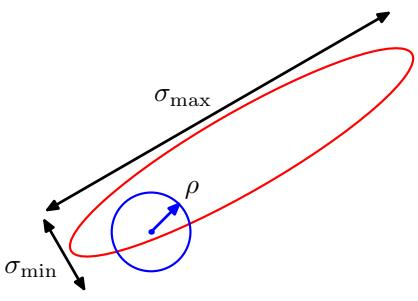
\includegraphics[keepaspectratio,alt={image}]{images/c1eaa05d311b422976d9e44c28e95584c6881305cbe60a4c0bebed8bd4bb3c35.jpg}}

proportion of accepted transitions will be high, but progress through
the state space takes the form of a slow random walk leading to long
correlation times. However, if the variance parameter is large, then the
rejection rate will be high because, in the kind of complex problems we
are considering, many of the proposed steps will be to states for which
the probability \(p ( \mathbf { z } )\) is low. Consider a multivariate
distribution \(p ( \mathbf { z } )\) having strong correlations between
the components of \(\mathbf { z } ,\) as illustrated in Figure 11.10.
The scale \(\rho\) of the proposal distribution should be as large as
possible without incurring high rejection rates. This suggests that
\(\rho\) should be of the same order as the smallest length scale
\(\sigma _ { \mathrm { m i n } }\) . The system then explores the
distribution along the more extended direction by means of a random
walk, and so the number of steps to arrive at a state that is more or
less independent of the original state is of order
\(( \sigma _ { \operatorname* { m a x } } / \sigma _ { \operatorname* { m i n } } ) ^ { 2 }\)
. In fact in two dimensions, the increase in rejection rate as \(\rho\)
increases is offset by the larger steps sizes of those transitions that
are accepted, and more generally for a multivariate Gaussian the number
of steps required to obtain independent samples scales like
\(( \sigma _ { \mathrm { m a x } } / \sigma _ { 2 } ) ^ { 2 }\) where
\(\sigma _ { 2 }\) is the second-smallest standard deviation (Neal,
1993). These details aside, it remains the case that if the length
scales over which the distributions vary are very different in different
directions, then the Metropolis Hastings algorithm can have very slow
convergence.

\subsection{11.3. Gibbs Sampling}\label{gibbs-sampling}

Gibbs sampling (Geman and Geman, 1984) is a simple and widely applicable
Markov chain Monte Carlo algorithm and can be seen as a special case of
the Metropolis-Hastings algorithm.

Consider the distribution
\(p ( \mathbf { z } ) = p ( z _ { 1 } , \dots , z _ { M } )\) from which
we wish to sample, and suppose that we have chosen some initial state
for the Markov chain. Each step of the Gibbs sampling procedure involves
replacing the value of one of the variables by a value drawn from the
distribution of that variable conditioned on the values of the remaining
variables. Thus we replace \(z _ { i }\) by a value drawn from the
distribution
\(p ( \boldsymbol { z } _ { i } | \mathbf { z } _ { \backslash i } )\) ,
where \(z _ { i }\) denotes the \(i ^ { \mathrm { t h } }\) component of
\(\mathbf { z } ,\) and \(\mathbf { z } _ { \backslash i }\) denotes
\(z _ { 1 } , \dots , z _ { M }\) but with \(z _ { i }\) omitted. This
procedure is repeated either by cycling through the variables in some
particular order or by choosing the variable to be updated at each step
at random from some distribution.

For example, suppose we have a distribution
\(p ( z _ { 1 } , z _ { 2 } , z _ { 3 } )\) over three variables, and at
step \(\tau\) of the algorithm we have selected values
\(z _ { 1 } ^ { ( \tau ) } , \dot { z } _ { 2 } ^ { ( \tau ) }\) and
\(z _ { 3 } ^ { ( \tau ) }\) . We first replace
\(z _ { 1 } ^ { ( \tau ) }\) by a new value
\(z _ { 1 } ^ { ( \tau + 1 ) }\) obtained by sampling from the
conditional distribution

\[
p (z _ {1} | z _ {2} ^ {(\tau)}, z _ {3} ^ {(\tau)}).\tag{11.46}
\]

Next we replace \(z _ { 2 } ^ { ( \tau ) }\) by a value
\(z _ { 2 } ^ { ( \tau + 1 ) }\) obtained by sampling from the
conditiona distribution

\[
p (z _ {2} | z _ {1} ^ {(\tau + 1)}, z _ {3} ^ {(\tau)})\tag{11.47}
\]

so that the new value for \(z _ { 1 }\) is used straight away in
subsequent sampling steps. Then we update \(z _ { 3 }\) with a sample
\(z _ { 3 } ^ { ( \tau + 1 ) }\) drawn from

\[
p (z _ {3} | z _ {1} ^ {(\tau + 1)}, z _ {2} ^ {(\tau + 1)})\tag{11.48}
\]

and so on, cycling through the three variables in turn.

\subsection{Gibbs Sampling}\label{gibbs-sampling-1}

\begin{enumerate}
\def\labelenumi{\arabic{enumi}.}
\tightlist
\item
  Initialize \(\{z_{i}:i=1,\ldots,M\}\) 2. For \(\tau=1,\ldots,T\) :
\end{enumerate}

\begin{itemize}
\tightlist
\item
  Sample
  \(z_{1}^{(\tau+1)} \sim p(z_{1}|z_{2}^{(\tau)}, z_{3}^{(\tau)}, \ldots, z_{M}^{(\tau)})\)
  .
\item
  Sample
  \(z_{2}^{(\tau+1)} \sim p(z_{2}|z_{1}^{(\tau+1)}, z_{3}^{(\tau)}, \ldots, z_{M}^{(\tau)})\)
  . \(\vdots\) - Sample
  \(z_{j}^{(\tau+1)} \sim p(z_{j}|z_{1}^{(\tau+1)}, \ldots, z_{j-1}^{(\tau+1)}, z_{j+1}^{(\tau)}, \ldots, z_{M}^{(\tau)})\)
  . \(\vdots\) - Sample
  \(z_{M}^{(\tau+1)} \sim p(z_{M}|z_{1}^{(\tau+1)}, z_{2}^{(\tau+1)}, \ldots, z_{M-1}^{(\tau+1)})\)
  .
\end{itemize}

\pandocbounded{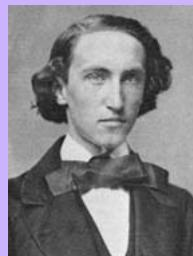
\includegraphics[keepaspectratio,alt={image}]{images/a69da9a2a027f83ff5571df636434b073fd7f442533c555dd07747d221b0a7af.jpg}}

\subsection{Josiah Willard Gibbs
1839--1903}\label{josiah-willard-gibbs-18391903}

Gibbs spent almost his entire life living in a house built by his father
in New Haven, Connecticut. In 1863, Gibbs was granted the first PhD in
engineering in the United States, and in 1871 he was appointed to

States at Yale, a post for which he received no salary because at the
time he had no publications. He developed the field of vector analysis
and made contributions to crystallography and planetary orbits. His most
famous work, entitled On the Equilibrium of Het-, laid the foundations
for the science of physical chemistry.

the first chair of mathematical physics in the United

To show that this procedure samples from the required distribution, we
first of all note that the distribution \(p ( \mathbf { z } )\) is an
invariant of each of the Gibbs sampling steps individually and hence of
the whole Markov chain. This follows from the fact that when we sample
from \(p ( z _ { i } | \{ \mathbf { z } _ { \backslash i } )\) , the
marginal distribution \(p ( \mathbf { z } _ { \backslash i } )\) is
clearly invariant because the value of
\(\mathbf { z } _ { \backslash i }\) is unchanged. Also, each step by
definition samples from the correct conditional distribution
\(p ( \boldsymbol { z } _ { i } | \mathbf { z } _ { \backslash i } )\) .
Because these conditional and marginal distributions together specify
the joint distribution, we see that the joint distribution is itself
invariant.

The second requirement to be satisfied in order that the Gibbs sampling
procedure samples from the correct distribution is that it be ergodic. A
sufficient condition for ergodicity is that none of the conditional
distributions be anywhere zero. If this is the case, then any point in z
space can be reached from any other point in a finite number of steps
involving one update of each of the component variables. If this
requirement is not satisfied, so that some of the conditional
distributions have zeros, then ergodicity, if it applies, must be proven
explicitly.

The distribution of initial states must also be specified in order to
complete the algorithm, although samples drawn after many iterations
will effectively become independent of this distribution. Of course,
successive samples from the Markov chain will be highly correlated, and
so to obtain samples that are nearly independent it will be necessary to
subsample the sequence.

We can obtain the Gibbs sampling procedure as a particular instance of
the Metropolis-Hastings algorithm as follows. Consider a
Metropolis-Hastings sampling step involving the variable \(z _ { k }\)
in which the remaining variables \(\mathbf { z } _ { \backslash k }\)
remain fixed, and for which the transition probability from z to
\(\mathbf { z } ^ { \star }\) is given by
\(q _ { k } ( \mathbf { \dot { z } } ^ { \star } \vert \mathbf { z } ) = p ( z _ { k } ^ { \star } \vert \mathbf { z } _ { \backslash k } )\)
We note that
\(\mathbf { z } _ { \mathrm { backslash } k } ^ { \star } = \mathbf { z } _ { \mathrm { \backslash } k }\)
because these components are unchanged by the sampling step. Also,
\(p ( \mathbf { z } ) = p ( z _ { k } | \mathbf { z } _ { \backslash k } ) p ( \mathbf { z } _ { \backslash k } )\)
. Thus the factor that determines the acceptance probability in the
Metropolis-Hastings (11.44) is given by

\[
A (\mathbf {z} ^ {\star}, \mathbf {z}) = \frac {p (\mathbf {z} ^ {\star}) q _ {k} (\mathbf {z} | \mathbf {z} ^ {\star})}{p (\mathbf {z}) q _ {k} (\mathbf {z} ^ {\star} | \mathbf {z})} = \frac {p (z _ {k} ^ {\star} | \mathbf {z} _ {\backslash k} ^ {\star}) p (\mathbf {z} _ {\backslash k} ^ {\star}) p (z _ {k} | \mathbf {z} _ {\backslash k} ^ {\star})}{p (z _ {k} | \mathbf {z} _ {\backslash k}) p (\mathbf {z} _ {\backslash k}) p (z _ {k} ^ {\star} | \mathbf {z} _ {\backslash k})} = 1\tag{11.49}
\]

where we have used
\(\mathbf { z } _ { \mathrm { ~ } k } ^ { \star } = \mathbf { z } _ { \backslash k }\)
. Thus the Metropolis-Hastings steps are always accepted.

As with the Metropolis algorithm, we can gain some insight into the
behaviour of Gibbs sampling by investigating its application to a
Gaussian distribution. Consider a correlated Gaussian in two variables,
as illustrated in Figure 11.11, having conditional distributions of
width l and marginal distributions of width L. The typical step size is
governed by the conditional distributions and will be of order l.
Because the state evolves according to a random walk, the number of
steps needed to obtain independent samples from the distribution will be
of order \(( L / \bar { l ) ^ { 2 } }\) . Of course if the Gaussian
distribution were uncorrelated, then the Gibbs sampling procedure would
be optimally efficient. For this simple problem, we could rotate the
coordinate system in order to decorrelate the variables. However, in
practical applications it will generally be infeasible to find such
transformations.

One approach to reducing random walk behaviour in Gibbs sampling is
called over-relaxation (Adler, 1981). In its original form, this applies
to problems for which

Figure 11.11

Illustration of Gibbs sampling by alternate updates of two variables
whose distribution is a correlated Gaussian. The step size is governed
by the standard deviation of the conditional distribution (green curve),
and is \(O ( l )\) , leading to slow progress in the direction of
elongation of the joint distribution (red ellipse). The number of steps
needed to obtain an independent sample from the distribution is
\(\dot { \cal O } ( ( L / l ) ^ { 2 } )\) ).

\pandocbounded{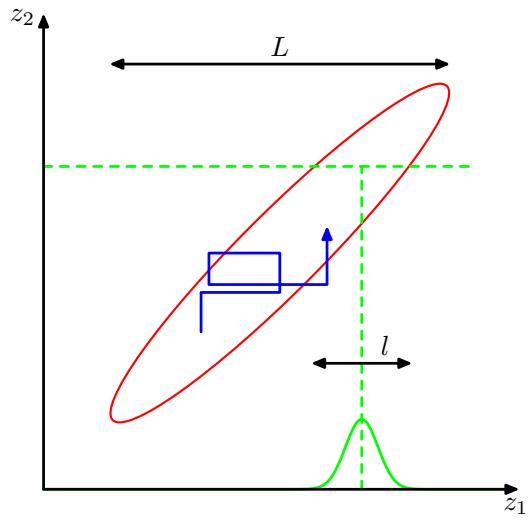
\includegraphics[keepaspectratio,alt={image}]{images/acbed698f58a05c63e5c1457e5c02a75bf173e39bd1882076c23582bd161d47b.jpg}}

the conditional distributions are Gaussian, which represents a more
general class of distributions than the multivariate Gaussian because,
for example, the non-Gaussian distribution
\(p ( z , y ) \propto \exp ( - z ^ { 2 } y ^ { 2 } )\) has Gaussian
conditional distributions. At each step of the Gibbs sampling algorithm,
the conditional distribution for a particular component \(z _ { i }\)
has some mean \(\mu _ { i }\) and some variance
\(\sigma _ { i } ^ { 2 }\) . In the over-relaxation framework, the value
of \(z _ { i }\) is replaced with

\[
z _ {i} ^ {\prime} = \mu_ {i} + \alpha (z _ {i} - \mu_ {i}) + \sigma_ {i} (1 - \alpha_ {i} ^ {2}) ^ {1 / 2} \nu\tag{11.50}
\]

where ν is a Gaussian random variable with zero mean and unit variance,
and α is a parameter such that \(- 1 < \alpha < 1\) . For \(\alpha = 0\)
, the method is equivalent to standard Gibbs sampling, and for
\(\alpha < 0\) the step is biased to the opposite side of the mean. This
step leaves the desired distribution invariant because if \(z _ { i }\)
has mean \(\mu _ { i }\) and variance
\(\sigma _ { i } ^ { \bar { 2 } }\) , then so too does
\(z _ { i } ^ { \prime } .\) . The effect of over-relaxation is to
encourage directed motion through state space when the variables are
highly correlated. The framework of ordered over-relaxation (Neal, 1999)
generalizes this approach to non-Gaussian distributions.

The practical applicability of Gibbs sampling depends on the ease with
which samples can be drawn from the conditional distributions
\(p ( \boldsymbol { z } _ { k } | \mathbf { z } _ { \backslash k } )\) .
In the case of probability distributions specified using graphical
models, the conditional distributions for individual nodes depend only
on the variables in the corresponding Markov blankets, as illustrated in
Figure 11.12. For directed graphs, a wide choice of conditional
distributions for the individual nodes conditioned on their parents will
lead to conditional distributions for Gibbs sampling that are log
concave. The adaptive rejection sampling methods discussed in Section
11.1.3 therefore provide a framework for Monte Carlo sampling from
directed graphs with broad applicability.

If the graph is constructed using distributions from the exponential
family, and if the parent-child relationships preserve conjugacy, then
the full conditional distributions arising in Gibbs sampling will have
the same functional form as the original conditional distributions
(conditioned on the parents) defining each node, and so standard
sampling techniques can be employed. In general, the full conditional
distributions will be of a complex form that does not permit the use of
standard sampling algorithms. However, if these conditionals are log
concave, then sampling can be done efficiently using adaptive rejection
sampling (assuming the corresponding variable is a scalar).

Figure 11.12 The Gibbs sampling method requires samples to be drawn from
the conditional distribution of a variable conditioned on the remaining
variables. For graphical models, this conditional distribution is a
function only of the states of the nodes in the Markov blanket. For an
undirected graph this comprises the set of neighbours, as shown on the
left, while for a directed graph the Markov blanket comprises the
parents, the children, and the co-parents, as shown on the right.

\pandocbounded{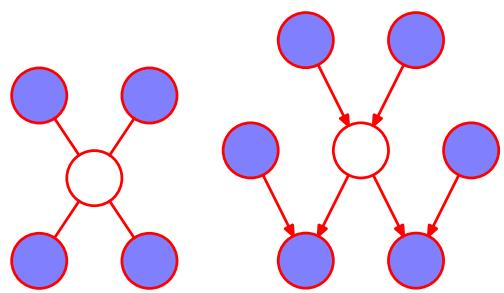
\includegraphics[keepaspectratio,alt={image}]{images/6b8c80cfb8a0a39f7a8b75952b26b40fdbd6cd5eec051d811eec42b0aaf10f4f.jpg}}

If, at each stage of the Gibbs sampling algorithm, instead of drawing a
sample from the corresponding conditional distribution, we make a point
estimate of the variable given by the maximum of the conditional
distribution, then we obtain the iterated conditional modes (ICM)
algorithm discussed in Section 8.3.3. Thus ICM can be seen as a greedy
approximation to Gibbs sampling.

Because the basic Gibbs sampling technique considers one variable at a
time, there are strong dependencies between successive samples. At the
opposite extreme, if we could draw samples directly from the joint
distribution (an operation that we are supposing is intractable), then
successive samples would be independent. We can hope to improve on the
simple Gibbs sampler by adopting an intermediate strategy in which we
sample successively from groups of variables rather than individual
variables. This is achieved in the blocking Gibbs sampling algorithm by
choosing blocks of variables, not necessarily disjoint, and then
sampling jointly from the variables in each block in turn, conditioned
on the remaining variables (Jensen et al., 1995).

\subsection{11.4. Slice Sampling}\label{slice-sampling}

We have seen that one of the difficulties with the Metropolis algorithm
is the sensitivity to step size. If this is too small, the result is
slow decorrelation due to random walk behaviour, whereas if it is too
large the result is inefficiency due to a high rejection rate. The
technique of slice sampling (Neal, 2003) provides an adaptive step size
that is automatically adjusted to match the characteristics of the
distribution. Again it requires that we are able to evaluate the
unnormalized distribution \(\widetilde { p } ( \mathbf { z } )\)

Consider first the univariate case. Slice sampling involves augmenting z
with an additional variable u and then drawing samples from the joint
(z, u) space. We shall see another example of this approach when we
discuss hybrid Monte Carlo in Section 11.5. The goal is to sample
uniformly from the area under the distribution

\pandocbounded{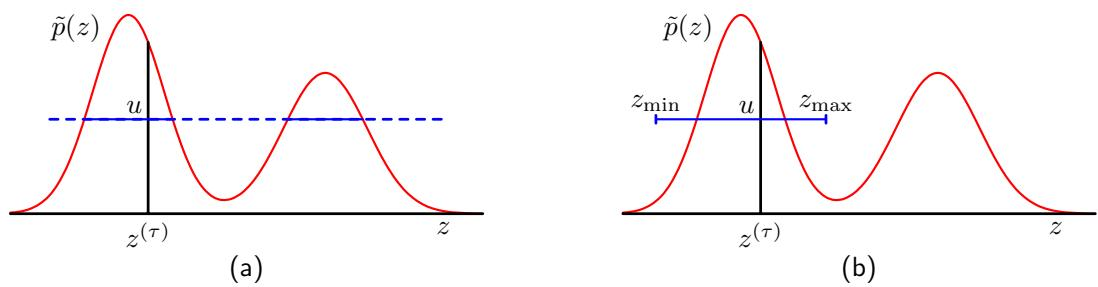
\includegraphics[keepaspectratio,alt={image}]{images/94e8a69b959b5c991b47c9071b4c8b1cf3c451fdd55b8a7bd3ebf9dacff73f7e.jpg}}

Figure 11.13 Illustration of slice sampling. (a) For a given value
\(z ^ { ( \tau ) }\) , a value of u is chosen uniformly in the region
\(0 \leqslant u \leqslant \widetilde { p } ( z ^ { ( \tau ) } )\) ,
which then defines a `slice' through the distribution, shown by the
solid horizontal lines. (b) Because it is infeasible to sample directly
from a slice, a new sample of z is drawn from a region zmin
\(\leqslant z \leqslant z _ { \mathrm { m a x } }\) , which contains the
previous value \(\dot { z } ^ { ( \tau ) }\)

given by

\[
\widehat {p} (z, u) = \left\{ \begin{array}{l l} 1 / Z _ {p} & \text { if } 0 \leqslant u \leqslant \widetilde {p} (z) \\ 0 & \text { otherwise } \end{array} \right.\tag{11.51}
\]

where \(Z _ { p } = \int \widetilde { p } ( z )\) dz. The marginal
distribution over \(z\) is given by

\[
\int \widehat {p} (z, u) \mathrm{d} u = \int_ {0} ^ {\widetilde {p} (z)} \frac {1}{Z _ {p}} \mathrm{d} u = \frac {\widetilde {p} (z)}{Z _ {p}} = p (z)\tag{11.52}
\]

and so we can sample from \(p ( z )\) by sampling from
\(\widehat { p } ( z , u )\) and then ignoring the u values. This can be
achieved by alternately sampling z and u. Given the value of \(z\) we
evaluate \(\widetilde { p } ( z )\) and then sample u uniformly in the
range \(0 \leqslant u \leqslant \widetilde { p } ( z )\) , which is
straightforward. Then we fix u and sample z uniformly from the `slice'
through the distribution defined by
\(\{ z : \widetilde { p } ( z ) > u \}\) . This is illustrated in Figure
11.13(a).

In practice, it can be difficult to sample directly from a slice through
the distribution and so instead we define a sampling scheme that leaves
the uniform distribution under \(\widehat { p } ( z , u )\) invariant,
which can be achieved by ensuring that detailed balance is satisfied.
Suppose the current value of z is denoted \(z ^ { ( \tau ) }\) and that
we have obtained a corresponding sample \(u .\) . The next value of z is
obtained by considering a region
\(z _ { \mathrm { m i n } } \leqslant z \leqslant z _ { \mathrm { m a x } }\)
that contains \(z ^ { ( \tau ) }\) . It is in the choice of this region
that the adaptation to the characteristic length scales of the
distribution takes place. We want the region to encompass as much of the
slice as possible so as to allow large moves in z space while having as
little as possible of this region lying outside the slice, because this
makes the sampling less efficient.

One approach to the choice of region involves starting with a region
containing \(z ^ { ( \tau ) }\) having some width w and then testing
each of the end points to see if they lie within the slice. If either
end point does not, then the region is extended in that direction by
increments of value w until the end point lies outside the region. A
candidate value \(z ^ { \prime }\) is then chosen uniformly from this
region, and if it lies within the slice, then it forms
\(z ^ { ( \tau + 1 ) }\) . If it lies outside the slice, then the region
is shrunk such that \(z ^ { \prime }\) forms an end point and such that
the region still contains \(\bar { z } ^ { ( \tau ) }\) . Then another
candidate point is drawn uniformly from this reduced region and so on,
until a value of z is found that lies within the slice.

Slice sampling can be applied to multivariate distributions by
repeatedly sampling each variable in turn, in the manner of Gibbs
sampling. This requires that we are able to compute, for each component
\(z _ { i } ,\) a function that is proportional to
\(p ( \boldsymbol { z } _ { i } | \mathbf { z } _ { \backslash i } )\)

\subsection{11.5. The Hybrid Monte Carlo
Algorithm}\label{the-hybrid-monte-carlo-algorithm}

As we have already noted, one of the major limitations of the Metropolis
algorithm is that it can exhibit random walk behaviour whereby the
distance traversed through the state space grows only as the square root
of the number of steps. The problem cannot be resolved simply by taking
bigger steps as this leads to a high rejection rate.

In this section, we introduce a more sophisticated class of transitions
based on an analogy with physical systems and that has the property of
being able to make large changes to the system state while keeping the
rejection probability small. It is applicable to distributions over
continuous variables for which we can readily evaluate the gradient of
the log probability with respect to the state variables. We will discuss
the dynamical systems framework in Section 11.5.1, and then in Section
11.5.2 we explain how this may be combined with the Metropolis algorithm
to yield the powerful hybrid Monte Carlo algorithm. A background in
physics is not required as this section is self-contained and the key
results are all derived from first principles.

\subsection{11.5.1 Dynamical systems}\label{dynamical-systems}

The dynamical approach to stochastic sampling has its origins in
algorithms for simulating the behaviour of physical systems evolving
under Hamiltonian dynamics. In a Markov chain Monte Carlo simulation,
the goal is to sample from a given probability distribution
\(p ( \mathbf { z } )\) . The framework of Hamiltonian dynamics is
exploited by casting the probabilistic simulation in the form of a
Hamiltonian system. In order to remain in keeping with the literature in
this area, we make use of the relevant dynamical systems terminology
where appropriate, which will be defined as we go along.

The dynamics that we consider corresponds to the evolution of the state
variable \(\mathbf { z } = \{ z _ { i } \}\) under continuous time,
which we denote by τ. Classical dynamics is described by Newton's second
law of motion in which the acceleration of an object is proportional to
the applied force, corresponding to a second-order differential equation
over time. We can decompose a second-order equation into two coupled
firstorder equations by introducing intermediate momentum variables
\(\mathbf { r } ,\) corresponding to the rate of change of the state
variables z, having components

\[
r _ {i} = \frac {\mathrm{d} z _ {i}}{\mathrm{d} \tau}\tag{11.53}
\]

where the \(z _ { i }\) can be regarded as position variables in this
dynamics perspective. Thus for each position variable there is a
corresponding momentum variable, and the joint space of position and
momentum variables is called phase space.

Without loss of generality, we can write the probability distribution
\(p ( \mathbf { z } )\) in the form 1

\[
p (\mathbf {z}) = \frac {1}{Z _ {p}} \exp (- E (\mathbf {z}))\tag{11.54}
\]

where \(E ( \mathbf { z } )\) is interpreted as the potential energy of
the system when in state z. The system acceleration is the rate of
change of momentum and is given by the applied force, which itself is
the negative gradient of the potential energy

\[
\frac {\mathrm{d} r _ {i}}{\mathrm{d} \tau} = - \frac {\partial E (\mathbf {z})}{\partial z _ {i}}.\tag{11.55}
\]

It is convenient to reformulate this dynamical system using the
Hamiltonian framework. To do this, we first define the kinetic energy by

\[
K (\mathbf {r}) = \frac {1}{2} \| \mathbf {r} \| ^ {2} = \frac {1}{2} \sum_ {i} r _ {i} ^ {2}.\tag{11.56}
\]

The total energy of the system is then the sum of its potential and
kinetic energies

\[
H (\mathbf {z}, \mathbf {r}) = E (\mathbf {z}) + K (\mathbf {r})\tag{11.57}
\]

where H is the Hamiltonian function. Using (11.53), (11.55), (11.56),
and (11.57), we can now express the dynamics of the system in terms of
the Hamiltonian equations given by

Exercise 11.15

\[
{\frac {\mathrm{d} z _ {i}}{\mathrm{d} \tau}} = {\frac {\partial H}{\partial r _ {i}}}\tag{11.58}
\]

\[
{\frac {\mathrm{d} r _ {i}}{\mathrm{d} \tau}} = {- \frac {\partial H}{\partial z _ {i}}.}\tag{11.59}
\]

\pandocbounded{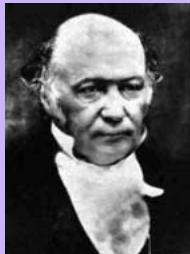
\includegraphics[keepaspectratio,alt={image}]{images/a01fad4437717ddbc077eb1966b6122e067b28a5016cdbecafd9f1c62e5f0ede.jpg}}

\subsection{William Hamilton
1805--1865}\label{william-hamilton-18051865}

William Rowan Hamilton was an Irish mathematician and physicist, and
child prodigy, who was appointed Professor of Astronomy at Trinity
College, Dublin, in 1827, before he had even graduated. One of
Hamilton's most important contributions was a new formulation of
dynamics, which played a significant role in the later development of
quantum mechanics.

His other great achievement was the development of , which generalize
the concept of complex numbers by introducing three distinct square
roots of minus one, which satisfy
\(i ^ { 2 } = j ^ { 2 } = k ^ { 2 } \stackrel { \cdot } { = } i j k = - 1 .\)
It is said that these equations occurred to him while walking along the
Royal Canal in Dublin with his wife, on 16 October 1843, and he promptly
carved the equations into the side of Broome bridge. Although there is
no longer any evidence of the carving, there is now a stone plaque on
the bridge commemorating the discovery and displaying the quaternion
equations.

\end{document}
